\documentclass[11pt,a4paper]{article}

\usepackage[margin=2.5cm]{geometry}
\usepackage{amsmath}
\usepackage{amssymb}
\usepackage{amsthm}
\usepackage{graphicx}
% ---------------------------------------------------------------------------
%  tikzstyles.tex -- shared diagram configuration for the report.
%  Every figure in this report draws with these styles. Do not restyle locally.
%  Convention: the electric field is red, the magnetic field is blue,
%  primal (cell-complex) objects are solid black, dual objects are dashed.
% ---------------------------------------------------------------------------
\usepackage{tikz}
\usetikzlibrary{positioning,calc,arrows.meta,decorations.pathmorphing,decorations.markings,patterns,shapes.geometric,fit,backgrounds,matrix,3d}
\usepackage{pgfplots}
\pgfplotsset{compat=1.18}

\definecolor{efield}{RGB}{190,30,45}      % E / primal edges / voltages
\definecolor{hfield}{RGB}{25,85,170}      % H / B / dual faces / fluxes
\definecolor{meshgrey}{RGB}{120,120,120}
\definecolor{softgrey}{RGB}{235,235,235}

\tikzset{
  % --- geometry ------------------------------------------------------------
  mesh/.style      = {draw=meshgrey, line width=0.4pt},
  mesh thin/.style = {draw=meshgrey!70, line width=0.3pt},
  primal/.style    = {draw=black, line width=1.1pt},
  dual/.style      = {draw=hfield, line width=1.1pt, dash pattern=on 2.2pt off 1.6pt},
  brick/.style     = {draw=black!70, line width=0.5pt, fill=softgrey},
  face/.style      = {fill=hfield!14, draw=hfield!70, line width=0.6pt},
  % --- degrees of freedom --------------------------------------------------
  edof/.style      = {-{Stealth[length=3.2pt]}, draw=efield, line width=1.3pt},
  edot/.style      = {circle, fill=efield, inner sep=0pt, minimum size=2.6pt},
  bdot/.style      = {circle, fill=hfield, inner sep=0pt, minimum size=2.6pt},
  harrow/.style    = {-{Stealth[length=3.2pt]}, draw=hfield, line width=1.3pt},
  oparrow/.style   = {-{Stealth[length=2.8pt]}, draw=black!70, line width=0.6pt},
  % --- annotations ---------------------------------------------------------
  dimline/.style   = {draw=black!60, line width=0.4pt, {Stealth[length=2.6pt]}-{Stealth[length=2.6pt]}},
  callout/.style   = {draw=black!45, line width=0.4pt, rounded corners=1.5pt, fill=white, inner sep=2.2pt, font=\footnotesize},
  lbl/.style       = {font=\footnotesize, inner sep=1.5pt},
  % --- plots ---------------------------------------------------------------
  ref line/.style  = {draw=black!55, line width=0.5pt, densely dotted},
  model line/.style= {draw=black!75, line width=0.7pt},
  meas mark/.style = {only marks, mark=*, mark size=2.2pt, draw=efield, fill=efield},
}
\pgfplotsset{
  rpt axis/.style = {width=0.92\linewidth, height=0.42\linewidth, tick label style={font=\scriptsize},
                     label style={font=\small}, legend style={font=\scriptsize, draw=black!40},
                     axis line style={draw=black!70}, tick style={draw=black!70}},
}

\usepackage{booktabs}
\usepackage{array}
\usepackage{xcolor}
\usepackage{caption}
\usepackage{subcaption}
\usepackage{listings}
\usepackage[colorlinks,linkcolor=blue!50!black,urlcolor=blue!50!black,citecolor=blue!50!black]{hyperref}
\usepackage{microtype}
\usepackage{siunitx}
\usepackage{float}
\usepackage{enumitem}

\newcommand{\eps}{\varepsilon}
\newcommand{\dd}{\mathrm{d}}
\newcommand{\Em}{{M_{\eps}}}   \newcommand{\Mm}{{M_{\mu}}}   \newcommand{\Ms}{{M_{\sigma}}}
\newcommand{\Cmat}{\mathbf{C}}  \newcommand{\Gmat}{\mathbf{G}}  \newcommand{\Smat}{\mathbf{S}}
\newcommand{\R}{ℝ}         \newcommand{\Ohm}{\Omega}     \renewcommand{\unit}[1]{\,\mathrm{#1}} % siunitx already owns \unit
\newtheorem{definition}{Definition}  \newtheorem{proposition}{Proposition}  \newtheorem{remark}{Remark}

\title{emfit: a finite integration technique solver for computational electromagnetics\\
  \large A living technical report -- state of the implementation}
\author{Project EE}
\date{\today}

\begin{document}

\maketitle

\begin{abstract}
\noindent
\texttt{emfit} is a finite integration technique (FIT) solver for computational electromagnetics on structured
hexahedral grids. It implements the curl and divergence operators of the primal and dual cell complexes together
with the diagonal Hodge star matrices that carry the material parameters, so that the discrete Maxwell system
inherits the algebraic structure of the continuous one. The time-domain core is a leapfrog stepper that conserves
a discrete energy to round-off, and the eigenvalue path solves the cavity problem with a dense eigensolver. The
computed cavity frequencies converge at second order and lie within of order one percent of the analytic
rectangular-box spectrum on the coarse grids used in the examples. This report is a living document: it records
what is currently verified, what is known to fail, and what is merely planned.
\end{abstract}

\tableofcontents

\clearpage

\lstdefinestyle{python}{language=Python,basicstyle=\ttfamily\small,showstringspaces=false,frame=single,breaklines}

\section{Aims and scope}

\noindent\emph{Status: draft -- the purpose, the division of labour between the sections and the notation are
settled; the framing will be adjusted as milestones land.}

\texttt{emfit} is meant to be an engineer's tool rather than a demonstration of a method. Given a
three-dimensional structure -- a cavity, a piece of laminate, a patch of a printed circuit board -- together with
a description of the materials filling it, the tool should answer the questions an engineer actually asks: where
the field is, at which frequencies the structure rings, and how much power leaves through which port. The
discretisation used throughout is the finite integration technique (FIT) introduced by Weiland
\cite{weiland1977,weiland1996} and systematised, in the form adopted here, by Clemens and Weiland
\cite{clemens2001} and Schuhmann and Weiland \cite{schuhmann2001}. The rest of this report is about how far that
single sentence has been made true, and where it has not.

\subsection{What the tool is for}

Two high-frequency workflows set the direction of the work, and a third, low-frequency extension follows once
they are solid.

\begin{itemize}[leftmargin=1.4em,itemsep=2pt]
  \item \textbf{A general three-dimensional solver.} A box of (for now isotropic, lossless) material is excited by
        a soft current source, and the fields are stepped in time. What is wanted out of it is the ring-down
        spectrum of a cavity, field maps on a cut plane, and an energy balance that can be trusted because it is
        exact rather than merely small.
  \item \textbf{An antenna on a printed circuit board.} A driven structure with feed and load ports, from which
        scattering parameters and a radiation pattern are extracted. This is the commercially relevant case and
        it is the reason the roadmap insists on ports, on a near-to-far-field transform and on importing real
        geometry, rather than on ever larger toy cavities; the antenna-theory side of the acceptance tests
        follows \cite{balanis2016}.
  \item \textbf{A low-frequency extension.} Magnetoquasistatic eddy currents in laminations and conductors, and a
        time-parallel integrator for long transient runs. This is deliberately last: it shares the grid and the
        material layer, and nothing else.
\end{itemize}

\subsection{Why the finite integration technique}

The choice of method is not incidental; six properties carried the decision.

FIT discretises the \emph{integral} form of Maxwell's equations rather than the differential form. The unknowns
are line integrals of the electric and magnetic field along primal and dual edges, and surface integrals of flux
through primal and dual faces \cite{weiland1977,clemens2001}. Because the integral form is an exact statement
about any cell, not only about an infinitesimally small one, there is no Taylor expansion anywhere in the
derivation: the only step at which the discrete model departs from Maxwell's equations is the constitutive step,
where the material response is replaced by a matrix on the grid.

Topology is exact and \emph{metric free}. The discrete operators are incidence matrices whose entries are $0$ and
$\pm 1$ and nothing else, so the identities $\Cmat\Gmat = 0$ and $\Smat\Cmat = 0$ hold in integer arithmetic on
every grid, uniform or not. Refining one region of the domain therefore changes nothing but the metric, i.e.\ the
Hodge star; that is a property a general finite-element assembly does not give for free, and it is what makes
non-uniform meshing cheap here.

The scheme is energy conserving in a strong sense, made precise in the section on energy conservation and stability: the leapfrog update
has an exact discrete invariant, a mixed-state energy that includes a first-order cross term, and that invariant
is conserved at the level of round-off rather than merely bounded.

There is no linear system to solve in the time domain. The Hodge stars are diagonal, so a step is two sparse
matrix-vector products: the electric and magnetic unknowns update each other explicitly. No global matrix is
factored, no preconditioner is built, and no iterative tolerance has to be chosen -- which is why a step is cheap
enough that the time domain is a practical way to obtain a spectrum.

FIT is the parent of Yee's scheme \cite{yee1966}. On a uniform orthogonal grid with staggered unknowns the two
coincide, so fifty years of accumulated experience with finite-difference time-domain methods on dispersion,
stability and staircasing \cite{taflove2005} transfers directly, and the FIT derivation supplies the reason why
those properties hold.

The price is regularity. FIT lives on structured hexahedral grids, so a curved surface becomes a staircase.
Finite elements on unstructured tetrahedra, or edge elements in the sense of Bossavit \cite{bossavit1998} and
Whitney forms in the sense of \cite{jin2014}, fit geometry better but pay for it with a global sparse solve at
every step, or with an implicit formulation and its conditioning problems. For the class of problems this project
targets -- boxes, cavities, layered laminates, antennas over a finite ground plane -- the structured grid is not
a practical limitation, and the cheap explicit step is decisive.

\subsection{Scope of this report}

This is a living document. It records what is implemented, the mathematics the implementation rests on, and the
measured evidence for each claim; every number quoted in the validation section is asserted by a test in the
repository, so a claim that stops being true turns the suite red. Anything that is designed but not implemented is
confined to the Outlook and to \texttt{docs/roadmap.md}; it is not described here in the present
tense. Where the two disagree, the roadmap is authoritative for status and this report for method.

\subsection{Implemented and not yet implemented}

\begin{itemize}[leftmargin=1.4em,itemsep=2pt]
  \item[] \textbf{Working today.}
        Orthogonal grids with non-uniform spacing and their dual cell complexes (\texttt{emfit/grid.py},
        \texttt{emfit/operators.py}); the three topological operators with $\Cmat\Gmat = 0$ and $\Smat\Cmat = 0$
        exact, verified against hand-checked stencils; the diagonal Hodge stars $\Em$, $\Mm$ and $\Ms$; the
        assembled system \texttt{FITSystem} with PEC walls imposed as a constraint on the unknown vector; the
        explicit leapfrog stepper, whose mixed-state invariant drifts by $8.5\times10^{-16}$ relative over the
        $343$~ns ring-down of the example (1800 steps) and stays at the $10^{-15}$ level over 2000 steps of random
        fields; the sharp CFL bound, stable at $1.01$ times the limit and divergent at $1.02$; a soft current
        source with the power balance $P = \vec e\cdot\vec j$; a dense cavity eigensolver with static-mode
        filtering and an analytic rectangular-box reference; and a headless visualisation layer with a runnable
        example. The suite is $336$ tests in $24$ modules; the fast selection runs $327$ of them in about
        $17$~s and deselects $9$ slow ones.
  \item[] \textbf{Measured accuracy.} On a $1.0\times0.7\times0.5$~m PEC box the first six modes are reproduced
        with a mean absolute error of $1.213\,\%$ and a maximum of $1.390\,\%$ on the $10\times7\times5$ grid, and
        $0.615\,\%$ / $0.711\,\%$ on $14\times10\times7$ -- a mean-error ratio of $0.507$ against the $0.510$
        predicted by second order for the $1.4$ times refinement used.
  \item[] \textbf{Absorbing boundaries, in part.} The first-order condition of G.~Mur \cite{mur1981} is
        implemented and measured (Section~\ref{sec:res-abc}): an outgoing pulse is absorbed to the level the
        discretisation allows, so a domain need no longer be closed by PEC or PMC walls. A matched lossy layer
        stands in for the perfectly matched layer of \cite{berenger1994} and is implemented too
        (Section~\ref{sec:res-pml}): it absorbs far more deeply than the condition does on the same geometry,
        but a layer of finite-difference cells is not a perfect match, and the acceptance criterion attached to
        it is not met. The near-to-far-field transform is implemented and checked against a closed-form source,
        and a bistatic scattering width computed through it has been set beside a Mie series
        (Section~\ref{sec:res-scatter}), though the agreement the milestone asks for has not been reached.
        Waveguide ports and S-parameters remain unavailable, and with them every input impedance.
  \item[] \textbf{Not implemented.} Geometry import from a board layout. A large-grid eigensolver, the dense
        path refusing more than 3000 free edges. Magnetoquasistatic eddy currents and time-parallel
        integration. Lossy and dispersive media: $\Ms$ is assembled but not yet coupled into the step, and
        the material layer understands diagonal tensors only. There is no non-orthogonal grid and no
        finite-element path; the two-dimensional studies of Section~\ref{sec:results} are the transverse-magnetic
        case of a grid one cell thick in the normal direction, which is what a single cell gives.
\end{itemize}

\subsection{Notation and conventions}

\begin{table}[H]
  \centering
  \caption{Symbols used throughout. The unit is the unit of the corresponding discrete quantity, which is what
  the code stores; the continuum field is the integrand, not the unknown.}
  \label{tab:notation}
  \begin{tabular}{@{}lll@{}}
    \toprule
    Symbol & Meaning & Unit \\
    \midrule
    $\vec e$      & electric field strength            & V/m   \\
    $\vec h$      & magnetic field strength            & A/m   \\
    $\vec b$      & magnetic flux density              & Wb/m$^2$ \\
    $\vec d$      & electric flux density              & C/m$^2$ \\
    $\vec j$      & electric current density           & A/m$^2$ \\
    $\Em$         & diagonal Hodge star, permittivity  & F     \\
    $\Mm$         & diagonal Hodge star, permeability  & H     \\
    $\Cmat$       & primal curl (faces $\times$ edges) & 1     \\
    $\Gmat$       & primal gradient (edges $\times$ nodes) & 1 \\
    $\Smat$       & primal divergence (cells $\times$ faces) & 1 \\
    $\eps_0$      & vacuum permittivity                & F/m   \\
    $\mu_0$       & vacuum permeability                & H/m   \\
    $c_0$         & vacuum speed of light              & m/s   \\
    \bottomrule
  \end{tabular}
\end{table}

\begin{itemize}[leftmargin=1.4em,itemsep=2pt]
  \item SI units throughout, with no unitless rescaling anywhere in the code: lengths in metres, energies in
        joules, powers in watts. All internal quantities are \texttt{float64}.
  \item Real-valued time-domain fields everywhere except in the eigenmode analysis, where complex phasors are used; the phasor convention is stated there where it
        matters and nowhere else.
  \item Degrees of freedom are written as bold lower case letters, and a tilde marks a quantity on the dual
        complex: $\mathbf{e}$, $\mathbf{h}$, and $\tilde{\mathbf{h}}$ for the dual line integral of $\vec h$.
  \item Unknown vectors are the concatenation \texttt{EX}, \texttt{EY}, \texttt{EZ} of the primal edges, then
        \texttt{FX}, \texttt{FY}, \texttt{FZ} of the primal faces, with each block flattened in C order; material
        vectors are indexed exactly like the block they belong to, not like the cells.
  \item Three dimensions only. There is no two-dimensional transverse-magnetic reduction, and every statement in
        this report is about a hexahedral complex.
\end{itemize}
      % \section{Aims and scope}
% ---------------------------------------------------------------------------
%  sec_howitworks.tex -- how the machine works: the bricks, the unknowns and
%  the curl matrix. Sits between the aims and the formal FIT section.
% ---------------------------------------------------------------------------
\section{How the machine works}\label{sec:howitworks}

This section is the tour we would give a colleague who wants to know what the solver does before reading the
formal statement of it. It describes the geometry the program sees, the numbers it stores on that geometry, and
the single matrix that turns a statement about one loop into a statement about every loop at once. There is no
derivation here and nothing is measured: the derivation is in Section~\ref{sec:theory}, and the evidence that
back the claims below is in the section on the discrete energy identity and in the section on the cavity
resonances. Nothing in this section is approximate except one thing, which we will point at when we come to it,
and that thing is the material. The topology -- what touches what, which edge bounds which face, what a loop
integral means -- is either right or wrong, and in this discretisation it is right.

\subsection{A box, cut into bricks}\label{sec:hiw:bricks}

The computational domain is a box, and the first decision, the one everything else follows from, is to cut it
into bricks. A brick is $\Delta x$ by $\Delta y$ by $\Delta z$; the three spacings may differ, and they may
differ from one brick to the next, but every brick is a box and every internal brick face is shared, whole, with
the face of exactly one neighbour. There is no other geometry in the program. The solver does not know that the
thing inside the box is a cavity with a fillet in one corner or a patch of laminate; it knows the bricks, the
numbering of their edges and faces, and which faces have been marked as conductor. When we say that a structure
has been discretised, this is the entirety of what we mean.

A single brick has eight corners, twelve edges and six faces. Interior faces are shared by two bricks and
interior edges by four, and it is that sharing rather than the brick itself which fixes the counts. For a mesh
of $N$ bricks there are, to within boundary terms that do not change the picture, $N$ corners, $3N$ edges and
$3N$ faces. The corners are the vertices, the edges join them, the faces are spanned by the edges and the bricks
are the cells the faces enclose; Figure~\ref{fig:hiw:brick} draws one brick in this reading.

Two of those counts are equal, and that is the first thing worth pausing on. A mesh with $3N$ edges has $3N$
faces, not approximately and not only when the bricks are cubes. It is the discrete form of the exact sequence
that runs vertices to edges to faces to cells in the continuum, where the boundary of a face is a loop of edges
and the boundary of a cell is a closed surface of faces, and where there is nothing left over at either end.
The practical consequence is that there are no spare slots and no choice about where the field goes. It has to
live on the edges and on the faces, because those are the entities whose counts match; an electric field held
at the corners would be short of unknowns by a factor of three in every direction, and there would be no loop
for Faraday's law to be written on.

What the solver knows of geometry is therefore the mesh and nothing else. A perfect electric conductor is a set
of faces marked as such, and the four edges bounding each of those faces are known quantities rather than
extrapolated ones. There is no analytic surface anywhere in the code to be intersected or sampled, which is why
the same code path takes a mesh with unequal spacings in all three directions without any change of
formulation. The shape of the object enters once, through the mesh; given the mesh, everything below is exact.

\begin{figure}[htbp]
\centering
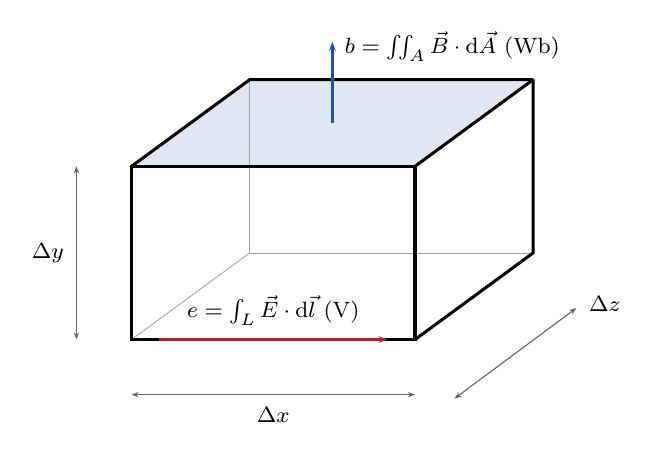
\begin{tikzpicture}[font=\footnotesize]
  % the shaded face: the top of the brick
  \draw[face] (0,2.2) -- (3.6,2.2) -- (5.1,3.3) -- (1.5,3.3) -- cycle;
  % the three edges hidden behind the body, left thin
  \draw[mesh thin] (0,0) -- (1.5,1.1);
  \draw[mesh thin] (1.5,1.1) -- (5.1,1.1);
  \draw[mesh thin] (1.5,1.1) -- (1.5,3.3);
  % the nine visible edges
  \draw[primal] (0,0) -- (3.6,0) -- (3.6,2.2) -- (0,2.2) -- cycle;
  \draw[primal] (3.6,0) -- (5.1,1.1) -- (5.1,3.3);
  \draw[primal] (3.6,2.2) -- (5.1,3.3);
  \draw[primal] (0,2.2) -- (1.5,3.3) -- (5.1,3.3);
  % one edge unknown
  \draw[edof] (0.35,0) -- (3.25,0);
  \node[lbl, anchor=south] at (1.8,0.12) {$e=\int_L \vec E\cdot \mathrm{d}\vec l\ (\si{\volt})$};
  % one face unknown and the direction of its normal
  \draw[harrow] (2.55,2.75) -- (2.55,3.78);
  \node[lbl, anchor=west] at (2.65,3.72) {$b=\iint_A \vec B\cdot \mathrm{d}\vec A\ (\si{\weber})$};
  % dimensions
  \draw[dimline] (0,-0.7) -- (3.6,-0.7);
  \node[lbl, anchor=north] at (1.8,-0.8) {$\Delta x$};
  \draw[dimline] (-0.7,0) -- (-0.7,2.2);
  \node[lbl, anchor=east] at (-0.8,1.1) {$\Delta y$};
  \draw[dimline] (4.1,-0.75) -- (5.65,0.4);
  \node[lbl, anchor=west] at (5.75,0.45) {$\Delta z$};
\end{tikzpicture}
\caption{One brick of a structured mesh, drawn in cabinet projection with the three hidden edges left thin so
that all twelve are accounted for. The unknown attached to an edge is the line integral of the electric field
along the whole edge, marked in red, and the unknown attached to a face is the flux of the magnetic field
through that face, marked in blue on the shaded top face. Neither mark is a point sample: the red arrow stands
for a definite integral along an edge, and the blue arrow gives the direction of a surface normal, nothing
more.}
\label{fig:hiw:brick}
\end{figure}

\subsection{What lives on an edge, and what lives on a face}\label{sec:hiw:dofs}

The unknown we store on an edge is not the electric field at some point of that edge. It is the line integral of
the electric field along the edge,
\begin{equation}
  e_i = \int_{L_i} \vec E \cdot \mathrm{d}\vec l ,
  \label{eq:hiw-e}
\end{equation}
in volts, and the unknown we store on a face is the surface integral of the magnetic flux density through it,
\begin{equation}
  b_j = \iint_{A_j} \vec B \cdot \mathrm{d}\vec A ,
  \label{eq:hiw-b}
\end{equation}
in webers. These two choices are the heart of the method, and they are not a convenience adopted to make the
algebra tidy.

Faraday's law is a statement about a loop and the surface the loop bounds; Ampere's law is a statement about a
loop and the surface that pierces it. If the unknowns are the integrals those laws are written in terms of,
then each law becomes a relation between unknowns with nothing in between: no quadrature, no interpolation, no
Taylor expansion, no assumption that the field is smooth across a brick. Note what the first equation is not. It
is not a point value of $E$ multiplied by a length; $E$ may vary arbitrarily along the edge and the integral
still means exactly what it says. The single number $e_i$ is all the solver ever knows about the field on that
edge, and on a given mesh it is all the solver needs.

There is a practical argument for the same choice. A voltmeter returns a line integral, and a loop of wire
returns the rate of change of a flux through a surface, so the quantities a measurement hands us are the
quantities stored here. A point value would be an interpolant, manufactured from the integrals whenever a plot
wanted one; the solver itself never needs it, because it goes from edge integrals to face integrals and back to
edge integrals without ever evaluating $E$ at a point. When we do draw a field map, the interpolation happens in
the plotting code, where it can be seen for what it is.

The two sets of unknowns do not share a home. The $e$ unknowns live on the edges, which form one lattice; the
$b$ unknowns live at the face centres, which form a second lattice displaced by half a brick in each of the
three directions. In two dimensions this is exactly the staggered grid of elementary finite-difference practice,
and Figure~\ref{fig:hiw:staggered} draws the two lattices on the same patch. Nothing is collocated: no $e$ and
no $b$ occupy the same location, and no two unknowns of any kind sit at the same point. This is a feature and
not an accident of implementation. The offset is what allows a difference of two neighbouring values to stand
for a derivative without ever pretending that two quantities defined at the same place can differ.

The offset also makes boundary conditions answerable. A perfect electric conductor is a set of marked faces, the
tangential electric field vanishes on those faces, and in these unknowns that is four numbers set to zero -- a
statement about a loop which is true by construction and needs no extrapolation from the interior.

\begin{figure}[htbp]
\centering
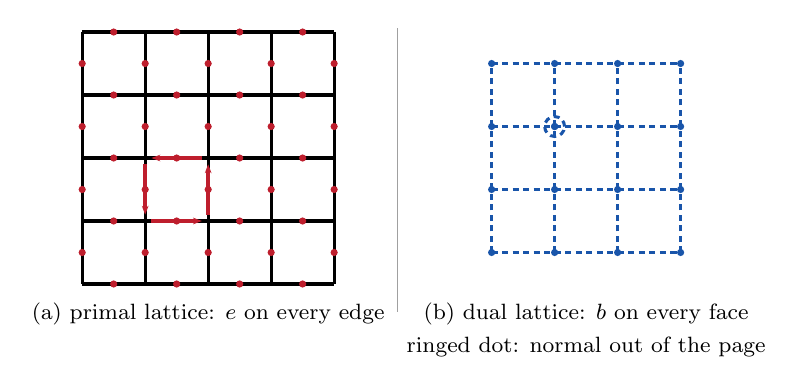
\begin{tikzpicture}[font=\footnotesize]
  \def\s{0.8}
  % (a) the primal lattice and its edge unknowns
  \foreach \i in {0,...,4}{
    \draw[primal] ({\i*\s},0) -- ({\i*\s},{4*\s});
    \draw[primal] (0,{\i*\s}) -- ({4*\s},{\i*\s});
  }
  \foreach \j in {0,...,4}{
    \foreach \i in {0,...,3}{
      \node[edot] at ({(\i+0.5)*\s},{\j*\s}) {};
      \node[edot] at ({\j*\s},{(\i+0.5)*\s}) {};
    }
  }
  \draw[edof] ({1.1*\s},{1*\s}) -- ({1.9*\s},{1*\s});
  \draw[edof] ({2*\s},{1.1*\s}) -- ({2*\s},{1.9*\s});
  \draw[edof] ({1.9*\s},{2*\s}) -- ({1.1*\s},{2*\s});
  \draw[edof] ({1*\s},{1.9*\s}) -- ({1*\s},{1.1*\s});
  \node[lbl, anchor=north] at ({2*\s},-0.18) {(a) primal lattice: $e$ on every edge};
  % separator
  \draw[mesh thin] (4.0,-0.35) -- (4.0,{4*\s+0.05});
  % (b) the dual lattice, shifted by half a cell
  \begin{scope}[xshift=4.8cm]
    \foreach \i in {0,...,3}{
      \draw[dual] ({(\i+0.5)*\s},{0.5*\s}) -- ({(\i+0.5)*\s},{3.5*\s});
      \draw[dual] ({0.5*\s},{(\i+0.5)*\s}) -- ({3.5*\s},{(\i+0.5)*\s});
    }
    \foreach \j in {0,...,3}{
      \foreach \i in {0,...,3}{
        \node[bdot] at ({(\i+0.5)*\s},{(\j+0.5)*\s}) {};
      }
    }
    \draw[dual] ({1.5*\s},{2.5*\s}) circle (3.6pt);
    \node[bdot] at ({1.5*\s},{2.5*\s}) {};
    \node[lbl, anchor=north] at ({2*\s},-0.18) {(b) dual lattice: $b$ on every face};
    \node[lbl, anchor=north] at ({2*\s},-0.62) {ringed dot: normal out of the page};
  \end{scope}
\end{tikzpicture}
\caption{The two lattices in two dimensions, on the same four-by-four patch and at the same scale. In (a) the
primal lattice carries the field on every edge: the arrows are drawn on the edges of one cell and the dots sit
at the midpoints of all of them. In (b) the dual lattice, displaced by half a cell, carries the flux at the
centre of every face, one of which is ringed to show its normal pointing out of the page. The thing to look at
is that no red dot and no blue dot coincides.}
\label{fig:hiw:staggered}
\end{figure}

\subsection{The matrix whose entries are only ever plus one, minus one, or zero}\label{sec:hiw:curl}

Take one face of one brick and the four edges that bound it. Faraday's law for that face, written in the
integrals we have chosen, reads
\begin{equation}
  e_1 + e_2 + e_3 + e_4 = -\frac{\mathrm{d}}{\mathrm{d}t} \, b ,
  \label{eq:hiw-faraday-face}
\end{equation}
where the left-hand side is the circulation of $\vec E$ round the loop provided each $e_i$ is taken in the sense
in which the loop is traversed. Each edge of the mesh has a positive direction fixed once and for all by the
grid axes, so an edge whose stored direction agrees with the traversal contributes $+e_i$ and an edge that runs
against it contributes $-e_i$. That is the entire origin of the signs in this method. A sign is either right or
wrong; there is no third possibility for it to approximate.

Now do it for every face at once. Collect the edge unknowns into a column vector $\mathbf{e}$, one entry per
edge, and the face unknowns into a column vector $\mathbf{b}$, one entry per face. Each of the equations above
is a sum of a few entries of $\mathbf{e}$ with signs, and a sum of that kind is one row of a matrix multiplying
$\mathbf{e}$. The matrix is $\Cmat$: one row per face, one column per edge, with
\begin{equation}
  \Cmat_{ji} =
  \begin{cases}
    +1 & \text{edge $i$ bounds face $j$ and runs with its orientation,}\\
    -1 & \text{edge $i$ bounds face $j$ and runs against it,}\\
     0 & \text{edge $i$ does not bound face $j$,}
  \end{cases}
  \label{eq:hiw-C}
\end{equation}
and the whole of Faraday's law, for every face simultaneously, is the single equation
\begin{equation}
  \Cmat \mathbf{e} = -\frac{\mathrm{d}}{\mathrm{d}t}\,\mathbf{b} .
  \label{eq:hiw-faraday}
\end{equation}
Nothing has been truncated on the way to this line. It is the discrete statement, not a discretisation of one.

Ampere's law uses the same matrix read the other way,
\begin{equation}
  \Cmat^{\!\top} \mathbf{h} = \frac{\mathrm{d}}{\mathrm{d}t}\,\mathbf{d} + \mathbf{j} ,
  \label{eq:hiw-ampere}
\end{equation}
with $\mathbf{h}$ on the dual edges that pierce the primal faces, $\mathbf{d}$ on the dual faces that cross the
primal edges, and $\mathbf{j}$ the current through those dual faces. The transpose is not a second operator that
happens to look similar. It is the same incidence counted from the other side, because the two complexes
interlace: a dual edge pierces a primal face, and the four dual faces that cross the primal edges bounding that
face are exactly the dual faces which that dual edge bounds. The set of incidences is one set, and the entries
of $\Cmat^{\top}$ are the entries of $\Cmat$ -- still $\pm 1$, still zero.

Everything now follows from the sparsity pattern, and this is where the method earns its keep. Write $\Gmat$ for
the matrix that takes values at the vertices to differences along the edges; its entries are also only $\pm 1$
or $0$. Go round any closed loop of edges: each vertex is entered once and left once, so each vertex value is
added once and subtracted once, and the sum telescopes to nothing. Therefore
\begin{equation}
  \Cmat \Gmat = \mathbf{0} \qquad \text{and, one complex over,} \qquad \Smat \Cmat = \mathbf{0} ,
  \label{eq:hiw-identities}
\end{equation}
identically, for any mesh, with no remainder and no error term. These are the discrete curl-grad and div-curl
identities, and they are properties of the matrices rather than statements that become truer as the mesh is
refined. \emph{The topology is exact; the only approximation is the material.} The material is where the
approximation lives because the constitutive relations are the only place where a continuum has to be replaced
by a number: the entries of the material matrices are averages over a brick, and an average is a judgement about
a shape that the mesh resolves only coarsely.

The consequences are not separate results, they are that same sentence said three ways. The discrete energy
identity holds term by term rather than to within a truncation error, because the work done by the curl term
telescopes across the mesh exactly; in a lossless cavity the measured relative drift of the discrete energy is
at the level of $10^{-15}$, which is round-off and nothing else, as reported in Section~\ref{sec:energy}. The
cavity eigenvalues converge at second order, with a measured rate of $0.507$ against a predicted $0.510$ in
Section~\ref{sec:eigen}. We refer to those sections rather than repeat them, because the point being made here
is the shape of the argument: exact algebra, an error that can only enter through the material numbers, and a
convergence rate that follows.

It is fair to ask what all this buys, since on a Cartesian mesh the arithmetic that comes out is the arithmetic
Yee wrote down in 1966 -- the same neighbours, the same stencil, later the same leapfrog update. If a stencil
were all that was wanted, the finite-difference reading would have got there first and more cheaply. What the
integral derivation buys is meaning. Each unknown is a definite physical quantity with a unit attached, so a
boundary condition is a statement about a surface or a loop rather than about the first row of a stencil, and
averaging a material over a brick is a well-posed question with a right answer rather than an accident of which
point the stencil happened to sample. And the algebra survives a change of mesh shape: the same incidence
matrices, with the same identities, describe distorted or non-orthogonal cells, and only the material matrices
change. The finite-difference reading has no such continuation, because its stencil was written for a Cartesian
grid in the first place.

\begin{figure}[htbp]
\centering
\begin{minipage}[c]{0.50\linewidth}
\centering
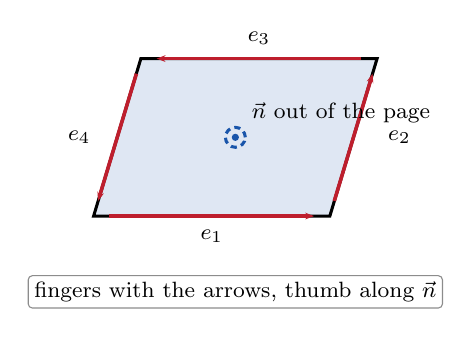
\begin{tikzpicture}[font=\footnotesize]
  \draw[face] (0,0) -- (3.0,0) -- (3.6,2.0) -- (0.6,2.0) -- cycle;
  \draw[primal] (0,0) -- (3.0,0) -- (3.6,2.0) -- (0.6,2.0) -- cycle;
  \draw[edof] (0.2,0) -- (2.8,0);
  \draw[edof] (3.057,0.192) -- (3.543,1.808);
  \draw[edof] (3.4,2.0) -- (0.8,2.0);
  \draw[edof] (0.543,1.808) -- (0.057,0.192);
  \node[lbl, anchor=north] at (1.5,-0.12) {$e_1$};
  \node[lbl, anchor=west]  at (3.68,1.0) {$e_2$};
  \node[lbl, anchor=south] at (2.1,2.12) {$e_3$};
  \node[lbl, anchor=east]  at (0.02,1.0) {$e_4$};
  \draw[dual] (1.8,1.0) circle (3.6pt);
  \node[bdot] at (1.8,1.0) {};
  \node[lbl, anchor=south west] at (1.95,1.12) {$\vec n$ out of the page};
  \node[callout, anchor=north] at (1.8,-0.75) {fingers with the arrows, thumb along $\vec n$};
\end{tikzpicture}
\end{minipage}\hfill
\begin{minipage}[c]{0.46\linewidth}
\centering
{\small
\[
\begin{bmatrix} +1 & +1 & -1 & -1 \end{bmatrix}
\begin{bmatrix} e_1 \\ e_2 \\ e_3 \\ e_4 \end{bmatrix}
= \oint_{\partial A} \vec E \cdot \mathrm{d}\vec l
\]}
{\footnotesize the four non-zeros of one row of $\Cmat$; every other column is zero.\par}
\end{minipage}
\caption{One face of a brick and the four edges that bound it, traversed anticlockwise as seen from the tip of
the normal. Faraday's law for this face is the scalar equation above: the four edge integrals added in the sense
of the arrows equal minus the rate of change of the flux through the face. Because each edge has a positive
direction fixed by the grid axes, two of the four run against their stored sense and enter with a minus sign,
and the row of $\Cmat$ beside the picture records that pattern. Reading the row against the edge vector
reproduces the circulation; stacking one row per face gives the matrix equation in the text.}
\label{fig:hiw:faraday}
\end{figure}

The three subsections above are the whole of the discretisation, and Figure~\ref{fig:hiw:sequence} puts them
into a single line. The entities form a chain -- vertices, edges, faces, cells -- and the operators run along it:
the gradient takes vertex values to differences along the edges, the curl takes edge integrals to face fluxes,
the divergence takes face fluxes to the net outflow from a cell. Every arrow in that chain is exact, in the sense
that its image is precisely the kernel of the next one; that is what the two identities assert, and each arrow is
a matrix whose entries are $+1$, $-1$ or $0$ and nothing else. That is the claim the rest of this report leans
on, and it is a claim about incidence rather than about resolution.

\begin{figure}[htbp]
\centering
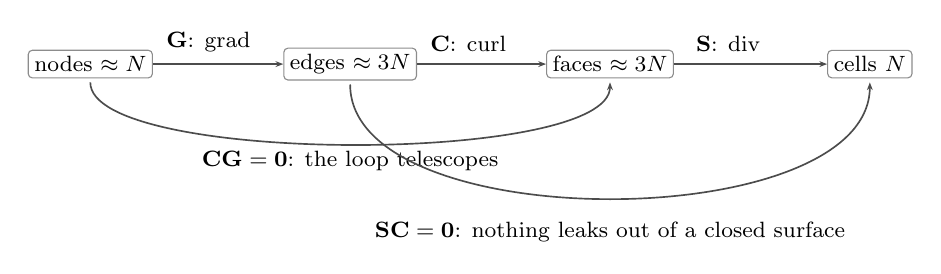
\begin{tikzpicture}[font=\footnotesize]
  \node[callout] (nd) at (0,0) {nodes $\approx N$};
  \node[callout] (ed) at (3.3,0) {edges $\approx 3N$};
  \node[callout] (fd) at (6.6,0) {faces $\approx 3N$};
  \node[callout] (cd) at (9.9,0) {cells $N$};
  \draw[oparrow] (nd.east) -- (ed.west);
  \draw[oparrow] (ed.east) -- (fd.west);
  \draw[oparrow] (fd.east) -- (cd.west);
  \node[lbl, anchor=south] at (1.5,0.10) {$\Gmat$: grad};
  \node[lbl, anchor=south] at (4.8,0.10) {$\Cmat$: curl};
  \node[lbl, anchor=south] at (8.1,0.10) {$\Smat$: div};
  \draw[oparrow] ($(nd.south)+(0,-0.05)$) .. controls ($(nd.south)+(0,-1.1)$) and ($(fd.south)+(0,-1.1)$) .. ($(fd.south)+(0,-0.05)$);
  \node[lbl, anchor=north] at (3.3,-1.05) {$\Cmat\Gmat=\mathbf{0}$: the loop telescopes};
  \draw[oparrow] ($(ed.south)+(0,-0.05)$) .. controls ($(ed.south)+(0,-2.0)$) and ($(cd.south)+(0,-2.0)$) .. ($(cd.south)+(0,-0.05)$);
  \node[lbl, anchor=north] at (6.6,-1.95) {$\Smat\Cmat=\mathbf{0}$: nothing leaks out of a closed surface};
\end{tikzpicture}
\caption{The chain of entities and the three operators that run along it, each with its matrix. The two
compositions underneath vanish identically. Read the picture as a statement about incidence and nothing else:
the loop integral of a gradient telescopes edge by edge, and the net flux of a curl out of a closed surface is
zero, for every mesh, because of what bounds what -- not because the mesh is fine.}
\label{fig:hiw:sequence}
\end{figure}

\subsection{Marching in time}\label{sec:hiw:leapfrog}

The two matrix equations have a property that is easy to miss and is the reason this is a time-domain method at
all. Faraday's law gives the rate of change of the face fluxes from the edge voltages and from nothing else;
Ampere's law gives the rate of change of the edge voltages from the face fluxes and the currents and from nothing
else. Each equation needs only the other family. So the two can be advanced in alternation: from the voltages at
one instant we update the fluxes, and from the updated fluxes we update the voltages. Neither half requires the
solution of a linear system, because the material matrices are diagonal, so every update is a division by a
number per unknown rather than an inversion of a matrix.

This is the trade the whole method makes, and it is worth naming the other side of it. A frequency-domain solver
inverts a large sparse matrix once per frequency and then has the whole spectrum; marching in time pays nothing
per step but must be run until the transient is over. What the time-domain route buys is the two things an
engineer usually wants from a structure of this kind: the response at every frequency at once, from one run, and
a field that can be watched while it evolves.

Written out, with $\mathbf{h}$ the magnetic field on the dual edges, $\mathbf{j}$ the current, and $\Delta t$ the
step,
\begin{equation}
  \begin{aligned}
    \mathbf{h}^{n+1/2} &= \mathbf{h}^{n-1/2} - \frac{\Delta t}{\mu}\,\Cmat\,\mathbf{e}^{n},\\
    \mathbf{e}^{n+1} &= \mathbf{e}^{n} + \frac{\Delta t}{\eps}\left(\Cmat^{\!\top}\mathbf{h}^{n+1/2}
       - \mathbf{j}^{n+1/2}\right).
  \end{aligned}
  \label{eq:hiw-leapfrog}
\end{equation}
The two families are offset by half a step -- the $\mathbf{h}$ values sit at $n\pm 1/2$ and the $\mathbf{e}$
values at $n$ -- which is where the name leapfrog comes from, and no unknown is ever updated from itself. That
is what keeps the scheme explicit and the storage down to two vectors per family.

The order of accuracy is second in time and second in space: halve the step and the brick and the error falls by
a factor of four. That is a statement about the method, and it is the reason the time step and the mesh have to
be refined together if the accuracy is to mean anything.

The step is not free. It is limited by the time light takes to cross the smallest brick, and in three dimensions
it is the diagonal of the brick that matters,
\begin{equation}
  \Delta t < \frac{\Delta x}{c\sqrt{3}} .
  \label{eq:hiw-courant}
\end{equation}
This bound is sharp, and it is worth being precise about how sharp. Measured on the implementation here, a run at
$1.01$ times the limit was stable and a run at $1.02$ times the limit diverged; Figure~\ref{fig:hiw:courant}
marks the two. Sharpness is a physical statement, not a numerical curiosity: below the bound the scheme does not
merely fail to blow up, it passes energy around consistently, one brick at a time; above it the update amplifies
what it is given and the field grows without bound.

The cost then follows by arithmetic rather than by measurement. In three dimensions, halving the brick gives
eight times the unknowns and halves the time step, so sixteen times the work per unit of simulated time. That is
the honest reason a method of this kind is used for one-off transient problems and for structures of a few
wavelengths, and not inside optimisation loops.

\begin{figure}[htbp]
\centering
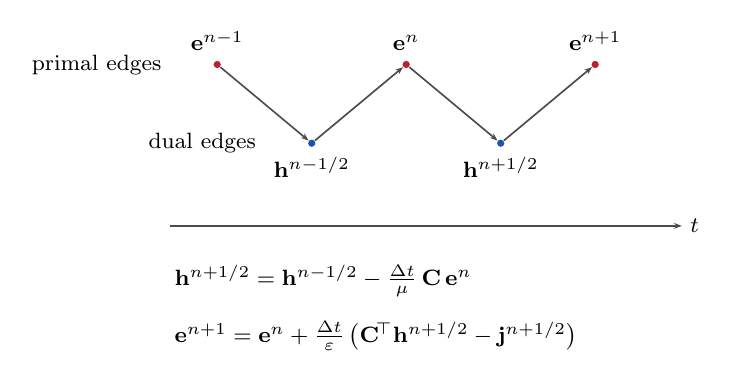
\begin{tikzpicture}[font=\footnotesize]
  \node[edot] (e1) at (2.0,1.0) {};
  \node[edot] (e2) at (4.4,1.0) {};
  \node[edot] (e3) at (6.8,1.0) {};
  \node[lbl, anchor=south] at (2.0,1.12) {$\mathbf{e}^{n-1}$};
  \node[lbl, anchor=south] at (4.4,1.12) {$\mathbf{e}^{n}$};
  \node[lbl, anchor=south] at (6.8,1.12) {$\mathbf{e}^{n+1}$};
  \node[bdot] (h1) at (3.2,0) {};
  \node[bdot] (h2) at (5.6,0) {};
  \node[lbl, anchor=north] at (3.2,-0.12) {$\mathbf{h}^{n-1/2}$};
  \node[lbl, anchor=north] at (5.6,-0.12) {$\mathbf{h}^{n+1/2}$};
  \draw[oparrow] (e1) -- (h1);
  \draw[oparrow] (h1) -- (e2);
  \draw[oparrow] (e2) -- (h2);
  \draw[oparrow] (h2) -- (e3);
  \node[lbl, anchor=east] at (1.35,1.0) {primal edges};
  \node[lbl, anchor=east] at (2.55,0) {dual edges};
  \draw[oparrow] (1.4,-1.05) -- (7.9,-1.05);
  \node[lbl, anchor=west] at (7.95,-1.05) {$t$};
  \node[lbl, anchor=west] at (1.4,-1.75) {$\mathbf{h}^{n+1/2}=\mathbf{h}^{n-1/2}-\frac{\Delta t}{\mu}\,\Cmat\,\mathbf{e}^{n}$};
  \node[lbl, anchor=west] at (1.4,-2.45) {$\mathbf{e}^{n+1}=\mathbf{e}^{n}+\frac{\Delta t}{\eps}\left(\Cmat^{\!\top}\mathbf{h}^{n+1/2}-\mathbf{j}^{n+1/2}\right)$};
\end{tikzpicture}
\caption{The two families on a time axis. The magnetic field sits at half-integer levels, the electric field at
integer ones, and each staircase arrow consumes only the other family: no arrow starts and ends in the same row.
Read the figure as the reason the update is explicit -- there is never a moment at which an unknown is asked for
its own future value.}
\label{fig:hiw:leapfrog}
\end{figure}

\begin{figure}[htbp]
\centering
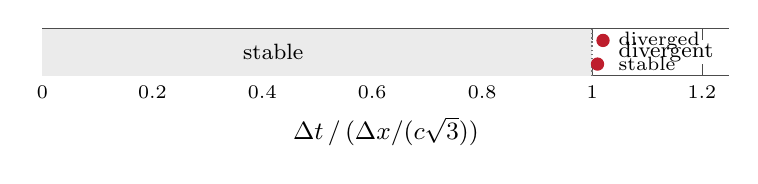
\begin{tikzpicture}[font=\footnotesize]
\begin{axis}[
  width=0.85\linewidth, height=0.18\linewidth,
  xmin=0, xmax=1.25, ymin=0, ymax=1,
  hide y axis, axis y line=none, ytick=\empty,
  xlabel={$\Delta t\,/\,(\Delta x/(c\sqrt{3}))$},
  tick label style={font=\scriptsize}, label style={font=\small},
  axis line style={draw=black!70}, tick style={draw=black!70},
  enlargelimits=false, clip=false,
]
  \fill[softgrey] (axis cs:0,0) rectangle (axis cs:1,1);
  \node[lbl] at (axis cs:0.42,0.5) {stable};
  \node[lbl, anchor=west] at (axis cs:1.04,0.5) {divergent};
  \draw[ref line] (axis cs:1,0) -- (axis cs:1,1);
  \addplot[only marks, mark=*, mark size=2.2pt, draw=efield, fill=efield]
    coordinates {(1.01,0.25) (1.02,0.75)};
  \node[lbl, anchor=west, font=\scriptsize] at (axis cs:1.04,0.25) {stable};
  \node[lbl, anchor=west, font=\scriptsize] at (axis cs:1.04,0.75) {diverged};
\end{axis}
\end{tikzpicture}
\caption{The stability bound as a hard edge rather than a rule of thumb. Everything to the left of the dotted
line is stable and nothing to the right of it is, as the two marks show: the time step that was stable sat at
$1.01$ times the limit and the next one, at $1.02$ times, diverged. There is no gradual degradation to trade
against -- the scheme either passes energy around consistently or it amplifies.}
\label{fig:hiw:courant}
\end{figure}

\subsection{What the machine is allowed to get wrong}\label{sec:hiw:materials}

The material enters the discrete problem through exactly two maps, $\mathbf{d}=\Em\mathbf{e}$ and
$\mathbf{b}=\Mm\mathbf{h}$, and nothing else. For a uniform material filling the whole box both matrices are
diagonal, and the update stays a division per unknown. Their entries are not simply the material constant,
however. In the diagonal case each entry carries the permittivity of its brick multiplied by a geometric factor,
the ratio of a face area to an edge length -- the cross-section of the dual cell to its length. That factor is
why a coarse mesh is wrong by a finite amount and a fine mesh converges: the material map is where the mesh
resolution actually enters the answer, and it is the only place it does.

An interface is where the difficulty sits. Put a brick of substrate against a brick of air and the edges lying in
the shared face belong to both; the discrete problem has one number to give each of them and they must be given
an average. Which average is a modelling decision, not a consequence of Maxwell's equations, and the choice is
visible in the result: two rules give answers that differ by amounts which do not shrink as the mesh is refined
unless the rule is the right one. The discontinuity in Figure~\ref{fig:hiw:interface} is real; the single value
the grid hands to an edge straddling it is a decision we make on the reader's behalf and should declare.

\emph{Every other ingredient on these pages is exact topology, and this is the only place where the discrete
problem is not the continuum problem.} Refining the mesh converges to the answer implied by the averaging rule
one has chosen, which is not necessarily the answer to Maxwell's equations.

That is not a technicality to be filed away. It is the question the later sections keep having to ask about
boxes and boundaries: the microstrip work in Section~\ref{sec:microstrip} cannot report a number without saying
what it did at the conductor edge, and the reference box in Section~\ref{sec:msres} is an attempt to make the
consequence of that choice measurable rather than assumed.

\begin{figure}[htbp]
\centering
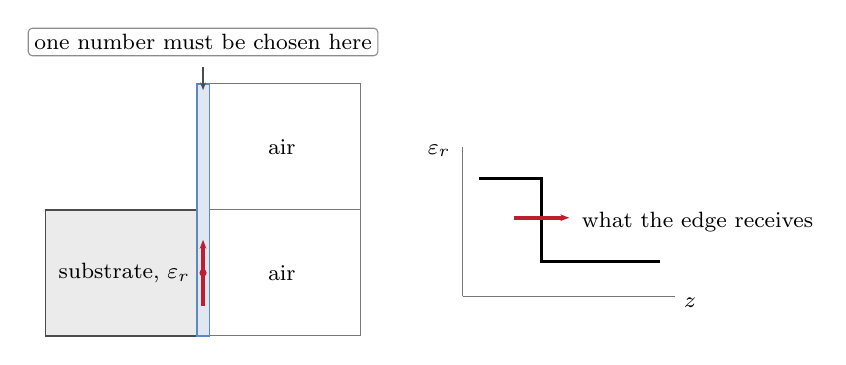
\begin{tikzpicture}[font=\footnotesize]
  \draw[brick] (0,0) rectangle (2,1.6);
  \node[lbl] at (1,0.8) {substrate, $\eps_r$};
  \draw[mesh] (2,0) rectangle (4,1.6);
  \node[lbl] at (3,0.8) {air};
  \draw[mesh] (2,1.6) rectangle (4,3.2);
  \node[lbl] at (3,2.4) {air};
  \fill[face] (1.92,0) rectangle (2.08,3.2);
  \draw[edof] (2,0.38) -- (2,1.22);
  \node[edot] at (2,0.8) {};
  \node[callout, anchor=south] at (2,3.55) {one number must be chosen here};
  \draw[oparrow] (2,3.42) -- (2,3.12);
  % inset: eps against z across the interface
  \draw[mesh] (5.3,0.5) -- (5.3,2.4);
  \draw[mesh] (5.3,0.5) -- (8.0,0.5);
  \node[lbl, anchor=east] at (5.2,2.35) {$\eps_r$};
  \node[lbl, anchor=west] at (8.05,0.42) {$z$};
  \draw[primal] (5.5,2.0) -- (6.3,2.0) -- (6.3,0.95) -- (7.8,0.95);
  \draw[edof] (5.95,1.5) -- (6.65,1.5);
  \node[lbl, anchor=west] at (6.75,1.45) {what the edge receives};
\end{tikzpicture}
\caption{A cross-section through three bricks with a substrate on the left and air on the right and above, and
the edge that lies in the interface picked out in red. The grid has exactly one number to hand that edge, drawn
as the dashed horizontal value in the inset, while the permittivity it is trying to represent jumps. Everything
that can be wrong in this method is in this picture; nothing in the topological half of it can be.}
\label{fig:hiw:interface}
\end{figure}

\subsection{Driving it: what a source is}\label{sec:hiw:source}

A source is nothing more than a current term. The update displayed in Section~\ref{sec:hiw:leapfrog} advances
the electric field from a curl of the magnetic field plus a current on the same edges, and the term
$\mathbf{j}^{n+1/2}$ in it is the whole of the mathematics. There is no excitation module, no injection
operator and no port object in the discrete problem: whatever launches a wave -- a feed, a line port, a plane
wave introduced through a total-field boundary -- arrives in the update as a current on a set of edges or, in
the dual update, as a magnetic current on a set of faces. The physics does not care which notation was used to
write that current down. The numbers do, because the two obvious ways of adding it behave differently towards
what comes back.

The first way is a hard source: overwrite the unknown on the driven edges with a prescribed value at every
step, so that the value on them is what was said and not what the neighbours computed. It is the shortest thing
to write in a test and it is a lie about the physics. An edge whose value is dictated cannot respond to the
field around it, and a tangential electric field held fixed at every instant is the boundary condition of a
perfect conductor by definition. The driven edge is a metal wall of our choosing: it radiates, which is why the
lie is easy to live with and why the run looks like a wave leaving a source, and it reflects everything that
returns to it. Use it to check a code against a closed-form answer -- the prescribed value is then a function
whose analytic field is already known -- and never to measure a device.

The second way is a soft source: add the current and leave the update alone. The value on the driven edge is
still computed from its neighbours; the current is one more term in the sum that produces it. The edge
therefore still obeys Maxwell, still feels the field that comes back to it, and is pushed back on by the wave
it launched. The consequence that matters is this: a soft source has an impedance, and it does not absorb what
comes back. Whatever travels back through the driven edge is reflected by it a second time, in phase or out of
it depending on that impedance, and re-radiated. A run driven by a soft source inside a closed test window
contains a standing wave by construction -- not because the solver is wrong, but because the source is in the
box with the wave.

Figure~\ref{fig:hiw:hardsoft} draws the two side by side. Neither behaviour is a defect to be repaired: it is
what the words ``driven by a source at this point'' mean. It does mean two things have to be declared wherever
a trace is shown, namely which of the two ways was used and where the source sat relative to every surface the
wave could return from. Section~\ref{sec:sp-definition} is where the same difficulty reappears in the language
of measurement: a scattering parameter is defined only when the incident wave is the only one arriving at the
port, and the terminations and reference planes are what make that true.

\begin{figure}[htbp]
\centering
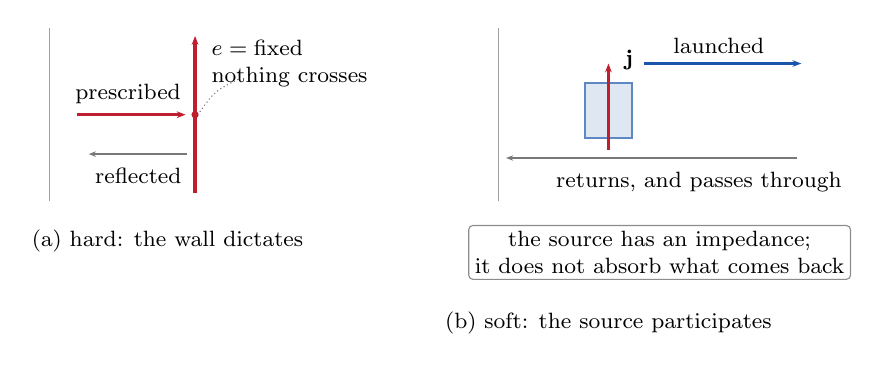
\begin{tikzpicture}[font=\footnotesize]
  % ---------------- (a) hard source ----------------
  \draw[mesh thin] (0.05,0.2) -- (0.05,2.4);
  \draw[edof] (1.9,0.3) -- (1.9,2.3);
  \node[edot] at (1.9,1.3) {};
  \node[lbl, anchor=west] at (2.05,2.15) {$e=\mathrm{fixed}$};
  \draw[edof] (0.4,1.3) -- (1.78,1.3);
  \node[lbl, anchor=south] at (1.05,1.38) {prescribed};
  \draw[meshgrey, line width=0.7pt, -{Stealth[length=2.6pt]}] (1.8,0.8) -- (0.55,0.8);
  \node[lbl, anchor=north] at (1.18,0.68) {reflected};
  \draw[mesh, densely dotted] (2.45,1.75) .. controls (2.15,1.6) .. (1.95,1.32);
  \node[lbl, anchor=west] at (2.05,1.78) {nothing crosses};
  \node[lbl, anchor=north] at (1.55,-0.1) {(a) hard: the wall dictates};
  % ---------------- (b) soft source ----------------
  \draw[mesh thin] (5.75,0.2) -- (5.75,2.4);
  \fill[face] (6.85,1.0) rectangle (7.45,1.7);
  \draw[edof] (7.15,0.85) -- (7.15,1.95);
  \node[lbl, anchor=west] at (7.3,2.0) {$\mathbf{j}$};
  \draw[harrow] (7.6,1.95) -- (9.6,1.95);
  \node[lbl, anchor=south] at (8.55,2.02) {launched};
  \draw[meshgrey, line width=0.7pt, -{Stealth[length=2.6pt]}] (9.55,0.75) -- (5.85,0.75);
  \node[lbl, anchor=north] at (8.3,0.63) {returns, and passes through};
  \node[callout, align=center, anchor=north] at (7.8,-0.1)
    {the source has an impedance;\\it does not absorb what comes back};
  \node[lbl, anchor=north] at (7.15,-1.15) {(b) soft: the source participates};
\end{tikzpicture}
\caption{The two ways of putting current into the update, drawn on the same edge. In (a) the value is
prescribed, so the edge is a metal wall: the field behind it cannot reach the unknown and what returns is
reflected. In (b) the current is added and the edge computes its own value, so the charge on it obeys its own
update and the returning wave passes through the source and continues rather than bouncing off it.}\label{fig:hiw:hardsoft}
\end{figure}

\subsection{Walls: what a box does to a wave}\label{sec:hiw:walls}

Every calculation in this report happens in a box, and a box has walls. A wall is a modelling decision of
exactly the same standing as the material average of Section~\ref{sec:hiw:materials}: the physics that comes
out is the physics of the box that was chosen, and a box is not free space. The walls are not a wrapper around
the real problem, added for the convenience of the solver; they are part of the problem, and a number taken
inside them is a number about the box as much as about the device.

Three kinds of wall are used, and each is worth stating twice -- once as what it does to the fields at the
wall, once as what it does to a wave arriving normally.

A perfect electric conductor sets the tangential electric field to zero. Nothing penetrates it, the surface
carries a current sheet, and the wave is reflected entirely with coefficient $\Gamma=-1$: the electric field of
the reflected wave points opposite to that of the incident one. A box lined with these is a cavity, so its
spectrum is discrete rather than continuous. On the grid the wall is the cheapest object there is: set the
tangential edges that lie on it to zero and never update them.

A perfect magnetic conductor sets the tangential magnetic field to zero instead. It is an open circuit rather
than a short, $\Gamma=+1$, and the electric field comes back in phase. No material is a magnetic wall at
microwave frequencies, and precisely that is what makes one useful. A structure symmetric about a plane can be
cut in half and the plane replaced by a wall -- which of the two walls it becomes depends only on whether the
drive is symmetric or antisymmetric about that plane. The full answer is then the half answer continued
across, at half the cost, and the wall is exact rather than approximate, because it encodes a symmetry of the
problem and not a property of any material.

A perfectly matched layer is not a boundary condition at all. It is a region of artificial loss, ideally
reflectionless, made by continuing the coordinates into the complex plane -- a complex coordinate stretch. The
reason it works is that a wave travelling in a coordinate with an imaginary part is attenuated while its
wavelength is unchanged, and because the stretch carries no frequency of its own the match is not tuned to a
band: it holds for whatever arrives, and the reflection does not grow as the layer is approached from any
angle. What the code implements is a conductivity profile whose strength ramps up over a few cells, with the
electric and magnetic losses held in the ratio that preserves the impedance of the medium; that ratio, not the
shape of the profile, is what does the matching.

A layer is only as good as its profile and its thickness, and both are choices rather than consequences. The
ramp in this work spans ten cells, which sits at the thin end of what is usual -- practice is commonly ten to
twenty -- and the thickness of the layer has never been swept here. That sentence is a statement about what has
not been measured, not about something known to be wrong, and it is the honest reason a wall reflection is
worth looking for in every trace.

Which is the practical point of this subsection. A wall reflection does not look like a phase error. It looks
like a standing wave: a ripple in the amplitude, with a period set by a length in the box rather than by
anything in the device, and it moves if the wall moves. A phase offset, by contrast, is a property of a
reference plane and travels with it. The diagnostic therefore needs no model at all -- if a curve ripples at a
period that matches a distance to a wall, the wall is talking, and the answer is a thicker layer or a farther
wall rather than a better description of the device. Figure~\ref{fig:hiw:walls} sets the three walls beside
one another; only the third returns nothing, and only the third is an approximation.

The formal treatment of the absorbing layer, its profile and the reflection it is measured to achieve, is in
Section~\ref{sec:res-pml}; the one-way condition it is compared against throughout is in
Section~\ref{sec:res-abc}.

\begin{figure}[htbp]
\centering
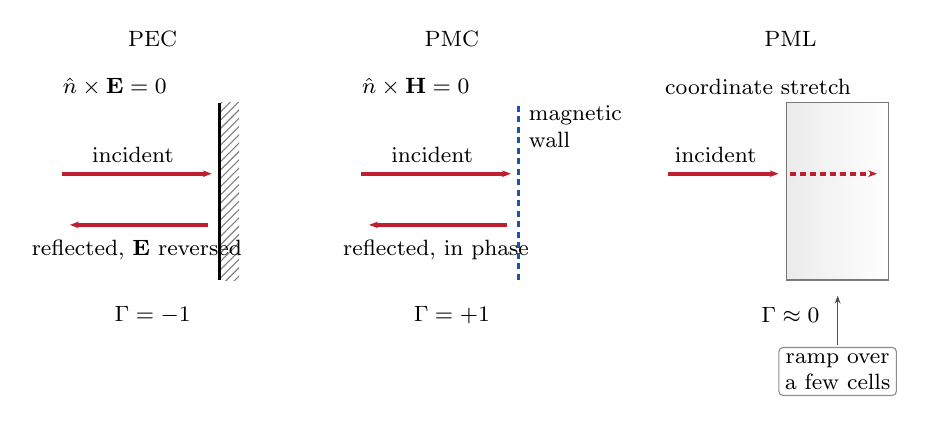
\begin{tikzpicture}[font=\footnotesize]
  % ---------------- PEC ----------------
  \draw[edof] (0.25,1.5) -- (2.15,1.5);
  \node[lbl, anchor=south] at (1.15,1.58) {incident};
  \fill[pattern=north east lines, pattern color=black!50] (2.25,0.15) rectangle (2.5,2.4);
  \draw[primal] (2.25,0.15) -- (2.25,2.4);
  \draw[edof] (2.1,0.85) -- (0.35,0.85);
  \node[lbl, anchor=north] at (1.2,0.72) {reflected, $\mathbf{E}$ reversed};
  \node[lbl, anchor=west] at (0.2,2.6) {$\hat{n}\times\mathbf{E}=0$};
  \node[lbl] at (1.4,-0.3) {$\Gamma=-1$};
  \node[lbl, anchor=south] at (1.4,3.05) {PEC};
  % ---------------- PMC ----------------
  \draw[edof] (4.05,1.5) -- (5.95,1.5);
  \node[lbl, anchor=south] at (4.95,1.58) {incident};
  \draw[dual] (6.05,0.15) -- (6.05,2.4);
  \node[lbl, anchor=west, align=left] at (6.12,2.1) {magnetic\\wall};
  \draw[edof] (5.9,0.85) -- (4.15,0.85);
  \node[lbl, anchor=north] at (5.0,0.72) {reflected, in phase};
  \node[lbl, anchor=west] at (4.0,2.6) {$\hat{n}\times\mathbf{H}=0$};
  \node[lbl] at (5.2,-0.3) {$\Gamma=+1$};
  \node[lbl, anchor=south] at (5.2,3.05) {PMC};
  % ---------------- PML ----------------
  \draw[edof] (7.95,1.5) -- (9.35,1.5);
  \node[lbl, anchor=south] at (8.55,1.58) {incident};
  \shade[left color=softgrey, right color=white] (9.45,0.15) rectangle (10.75,2.4);
  \draw[mesh] (9.45,0.15) rectangle (10.75,2.4);
  \draw[edof, dash pattern=on 2pt off 1.6pt] (9.5,1.5) -- (10.6,1.5);
  \node[lbl, anchor=west] at (7.85,2.6) {coordinate stretch};
  \node[lbl] at (9.5,-0.3) {$\Gamma\approx 0$};
  \node[lbl, anchor=south] at (9.5,3.05) {PML};
  \node[callout, align=center, anchor=north] at (10.1,-0.7) {ramp over\\a few cells};
  \draw[oparrow] (10.1,-0.68) -- (10.1,-0.05);
\end{tikzpicture}
\caption{Three walls and one wave arriving at each. The conductor reverses the electric field, the magnetic
wall returns it in phase, and the lossy ramp sends it into a coordinate that has an imaginary part and brings
nothing back. The first two are exact and visible in the answer; the third is the only one intended to be
invisible, and it is the only one that is an approximation.}\label{fig:hiw:walls}
\end{figure}


\subsection{Reading a number out: ports}\label{sec:hiw:ports}

A port is the place where it is decided what went in and what came out. There are two waves at a port, one
travelling in and one travelling out, and the measurement is the ratio of their amplitudes. Everything about
whether a number is quotable comes down to one question: can the port separate those two waves? If it cannot,
the ratio it reports is a mixture, and no amount of solver accuracy repairs a mixture.

The cheap construction is the lumped gap port. Leave a gap in the conductor, drive a current across it, read
the voltage as one line integral of the electric field across the gap -- a single edge -- and the current as
one loop integral of the magnetic field around the strip at that plane -- a single face loop. The impedance is
their ratio, $Z=V/I$, as drawn in Figure~\ref{fig:hiw:lumpedport}. This is a real measurement of the actual
fields at that plane, taken on the same unknowns the update produces; nothing is interpolated, fitted or
invented, and there is no hidden model between the field and the number.

It is not yet a scattering parameter, and the reason is intrinsic rather than numerical. $V$ and $I$ are two
different integrals over two different objects, an edge and a face loop, and their ratio equals the impedance
of a mode only if the field across the gap has exactly the transverse profile of that mode. A gap does not
excite a single profile. It excites a mixture, and the mixture evolves as it propagates: the components travel
at their own velocities and disperse, so the profile at the gap plane keeps changing, and it changes in
response to whatever comes back through it. $V/I$ therefore drifts as the profile evolves, and the drift is
contaminated by every other thing present at that plane, including whatever the box returns. That is a
statement about the port, not about the solver. The number is honest; it is simply not the number the device
is being asked about.

The construction that does give a scattering parameter is the modal port. Take the known transverse profile of
the mode, project the computed field at the port plane onto it -- a scalar product, an overlap integral -- then
inject only that amplitude going in and extract only that amplitude coming out. Now $V$ and $I$ are defined by
the projection rather than by one edge and one loop, and their ratio is a property of the mode rather than of
the gap. A modal port keeps one coefficient and discards the rest, and that discarding is what makes the
answer attributable to the device. The price is that the mode has to be known before the port can be built:
the profile calculation discussed with the power flow in Section~\ref{sec:sp-powerflow} is the thing that has
to have been done first, and in a guiding structure with an interface the profile is not something the
geometry alone will tell you.

One consequence has to be stated, because it governs how much a measured ratio can mean. Section~\ref{sec:hiw:source}
established that a soft source does not absorb the wave returning through it; inside a closed test window it
re-reflects that wave, so a forward and backward decomposition carried out in the same window sits on top of a
standing wave rather than on top of a travelling one. Any backward-to-forward ratio obtained that way is a
property of the source and the window as much as of the device between them, and the ambiguity does not
resolve with effort -- a finer mesh and a longer run both resolve the standing wave better without making it
smaller. What removes it is a port that separates the two waves by construction, together with walls that do
not return anything measurable (Section~\ref{sec:hiw:walls}).

The consequence for reading any number in this report is short. A scattering parameter is only as good as the
port that produced it, and ``the solver agreed with the analytic result'' has to mean the same port and the
same box on both sides of the comparison; otherwise the agreement is between two different questions that
happen to have similar answers.

\begin{figure}[htbp]
\centering
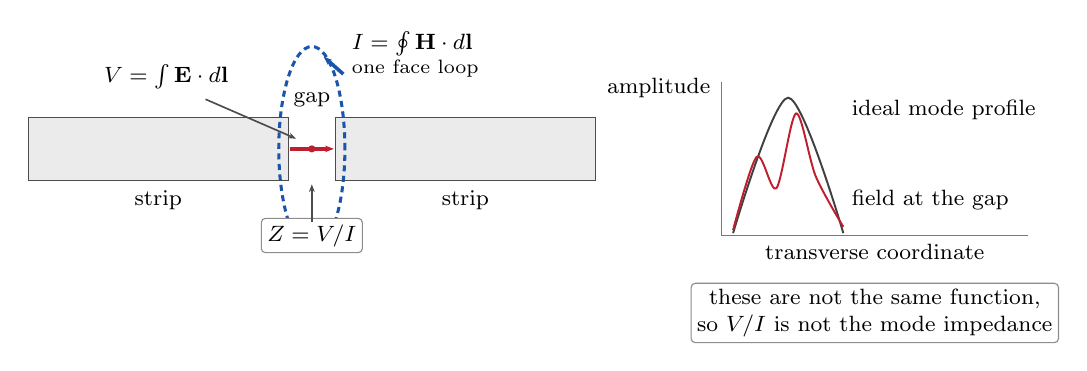
\begin{tikzpicture}[font=\footnotesize]
  % ---------------- the strip and its gap, seen from above ----------------
  \fill[brick] (0.3,1.25) rectangle (3.6,2.05);
  \fill[brick] (4.2,1.25) rectangle (7.5,2.05);
  \node[lbl, anchor=north] at (1.95,1.18) {strip};
  \node[lbl, anchor=north] at (5.85,1.18) {strip};
  \node[lbl, anchor=south] at (3.9,2.12) {gap};
  % one edge carries the voltage
  \draw[edof] (3.62,1.65) -- (4.18,1.65);
  \node[edot] at (3.9,1.65) {};
  \node[lbl, anchor=south] at (2.05,2.35) {$V=\int\mathbf{E}\cdot d\mathbf{l}$};
  \draw[oparrow] (2.55,2.28) -- (3.7,1.78);
  % one face loop carries the current
  \draw[dual] (3.9,1.65) ellipse [x radius=0.42, y radius=1.3];
  \draw[harrow] (4.3,2.6) -- (4.05,2.82);
  \node[lbl, anchor=west, align=left] at (4.35,2.85) {$I=\oint\mathbf{H}\cdot d\mathbf{l}$\\[-1pt]\scriptsize one face loop};
  \node[callout] at (3.9,0.55) {$Z=V/I$};
  \draw[oparrow] (3.9,0.72) -- (3.9,1.2);
  % ---------------- inset: the profile it assumes, and the one it has ----------------
  \draw[mesh] (9.1,0.55) -- (13.0,0.55);
  \draw[mesh] (9.1,0.55) -- (9.1,2.5);
  \draw[model line] plot[smooth] coordinates {(9.25,0.58) (9.95,2.3) (10.65,0.58)};
  \draw[efield, line width=0.7pt]
    plot[smooth] coordinates {(9.25,0.62) (9.55,1.55) (9.8,1.15) (10.05,2.1) (10.3,1.3) (10.65,0.66)};
  \node[lbl, anchor=west] at (10.7,2.15) {ideal mode profile};
  \node[lbl, anchor=west] at (10.7,1.0) {field at the gap};
  \node[lbl, anchor=east] at (9.02,2.42) {amplitude};
  \node[lbl, anchor=north] at (11.05,0.5) {transverse coordinate};
  \node[callout, align=center, anchor=north] at (11.05,-0.05)
    {these are not the same function,\\so $V/I$ is not the mode impedance};
\end{tikzpicture}
\caption{A lumped gap port. The voltage is one line integral across the gap and the current one loop integral
around the strip in the same plane, both taken on single grid objects, and the impedance is their ratio. The
inset is the assumption that ratio silently makes: that the profile at the gap is the profile of the mode. It
is not, which is why the number can be honest and still not be the one being asked for.}\label{fig:hiw:lumpedport}
\end{figure}

\begin{figure}[htbp]
\centering
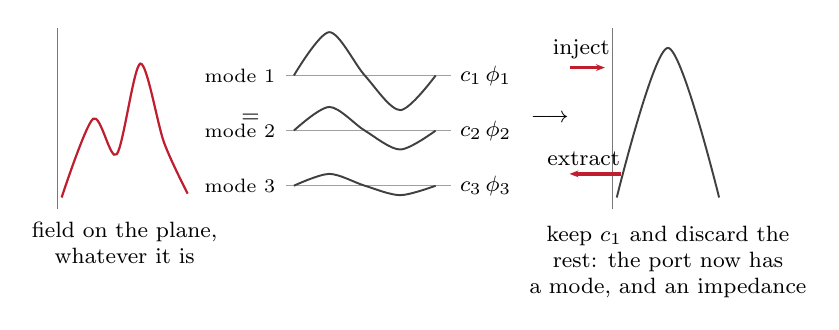
\begin{tikzpicture}[font=\footnotesize]
  % ---------------- (1) whatever the field happens to be ----------------
  \draw[mesh] (1.1,0.35) -- (1.1,2.65);
  \draw[efield, line width=0.8pt]
    plot[smooth] coordinates {(1.15,0.5) (1.55,1.5) (1.85,1.05) (2.15,2.2) (2.45,1.2) (2.75,0.55)};
  \node[lbl, anchor=north, align=center] at (1.95,0.25) {field on the plane,\\whatever it is};
  % ---------------- (2) the basis and its coefficients ----------------
  \node[lbl] at (3.55,1.5) {$=$};
  \foreach \k/\y/\a in {1/2.05/0.55, 2/1.35/0.3, 3/0.65/0.15} {
    \draw[mesh thin] (4.0,\y) -- (6.1,\y);
    \draw[model line] plot[smooth] coordinates
      {(4.1,\y) (4.55,{\y+\a}) (5.0,\y) (5.45,{\y-\a*0.8}) (5.9,\y)};
    \node[lbl, anchor=west] at (6.15,\y) {$c_{\k}\,\phi_{\k}$};
    \node[lbl, anchor=east] at (3.92,\y) {\scriptsize mode \k};
  }
  % ---------------- (3) one coefficient kept ----------------
  \node[lbl] at (7.35,1.5) {$\longrightarrow$};
  \draw[mesh] (8.15,0.35) -- (8.15,2.65);
  \draw[model line] plot[smooth]
    coordinates {(8.2,0.5) (8.85,2.4) (9.5,0.5)};
  \draw[edof] (7.6,2.15) -- (8.05,2.15);
  \node[lbl, anchor=south] at (7.75,2.2) {inject};
  \draw[edof] (8.25,0.8) -- (7.6,0.8);
  \node[lbl, anchor=south] at (7.78,0.85) {extract};
  \node[lbl, anchor=north, align=center] at (8.85,0.2)
    {keep $c_{1}$ and discard the\\rest: the port now has\\a mode, and an impedance};
\end{tikzpicture}
\caption{The modal port as a projection. The field actually present on the plane is an arbitrary function; the
mode basis resolves it into coefficients, of which the port keeps exactly one. Injecting and extracting that
one coefficient -- and refusing to see the others -- is what turns a pair of integrals into a property of the
mode, and it is why the mode has to be known before the port can be built.}\label{fig:hiw:modalport}
\end{figure}

 % \section{How the machine works}
\section{The finite integration technique}
\label{sec:theory}

\noindent\emph{Status: draft -- everything stated here is implemented and unit-tested; the derivation, the
motivating prose and the discussion of the non-orthogonal case are still being written.}

This section fixes the objects the implementation manipulates. It defines the two cell complexes of the grid, the
degrees of freedom as integrals over their elements, the three topological operators and the two identities they
satisfy exactly, the Maxwell grid equations, the diagonal Hodge stars that carry the material, and the way
boundary conditions and sources enter. The presentation follows Weiland \cite{weiland1977,weiland1996} and
\cite{clemens2001}; the energy and stability analysis that makes use of these objects is deferred to
the section on energy conservation and stability.

\subsection{The two cell complexes}

A structured hexahedral grid is the tensor product of three strictly increasing sequences of node coordinates,
$x_0 < \dots < x_{n_x}$, $y_0 < \dots < y_{n_y}$, $z_0 < \dots < z_{n_z}$. Its \emph{primal} objects are the
familiar ones: nodes at the corners, edges the segments joining adjacent nodes, faces the rectangles spanned by
two edges, cells the boxes spanned by three. Writing $n_k$ for the number of \emph{cells} along axis $k$, so that
axis $k$ carries $n_k+1$ nodes, the counts are those in Table~\ref{tab:counts}.

\begin{table}[H]
  \centering
  \caption{Entities of the primal and dual complexes of an $n_x\times n_y\times n_z$ grid, and their values for
  the $10\times7\times5$ cavity used in the validation runs.}
  \label{tab:counts}
  \begin{tabular}{@{}lrr@{}}
    \toprule
    Entity & Count & $10\times7\times5$ \\
    \midrule
    primal nodes   & $(n_x+1)(n_y+1)(n_z+1)$ & 528  \\
    primal edges   & $n_x(n_y+1)(n_z+1) + (n_x+1)n_y(n_z+1) + (n_x+1)(n_y+1)n_z$ & 1382 \\
    \quad of which $x$ & $n_x(n_y+1)(n_z+1)$ & 480 \\
    \quad of which $y$ & $(n_x+1)n_y(n_z+1)$ & 462 \\
    \quad of which $z$ & $(n_x+1)(n_y+1)n_z$ & 440 \\
    primal faces   & $(n_x+1)n_yn_z + n_x(n_y+1)n_z + n_xn_y(n_z+1)$ & 1205 \\
    \quad of which $x$ & $(n_x+1)n_yn_z$ & 385 \\
    \quad of which $y$ & $n_x(n_y+1)n_z$ & 400 \\
    \quad of which $z$ & $n_xn_y(n_z+1)$ & 420 \\
    primal cells   & $n_xn_yn_z$ & 350 \\
    dual nodes     & $n_xn_yn_z$ & 350 \\
    dual edges     & equal to the primal faces & 1205 \\
    dual faces     & equal to the primal edges & 1382 \\
    dual cells     & equal to the primal nodes & 528 \\
    \bottomrule
  \end{tabular}
\end{table}

The \emph{dual} complex is shifted by half a cell in every direction. A dual node sits at the centre of every
primal cell. A dual edge joins the two dual nodes on either side of a primal face and therefore \emph{pierces}
that face. A dual face spanned by the four dual edges around a primal edge therefore \emph{crosses} that edge. A
dual cell encloses a primal node and is bounded by the dual faces that cross the primal edges incident on that
node.

The counts in Table~\ref{tab:counts} are not an accident. For a single brick the alternating sum satisfies
\begin{equation}
  n_0 - n_1 + n_2 - n_3 = 528 - 1382 + 1205 - 350 = 1,
  \label{eq:euler}
\end{equation}
which is the Euler characteristic of a ball and holds for every grid; it is the reason the primal and dual counts
pair up as they do. In particular each dual edge threads exactly one primal face, and each dual face is pierced by
exactly one primal edge, so the pairing of primal and dual objects is a bijection. The implementation exploits
this: dual objects carry no indices of their own and are addressed by the primal object they are paired with,
which is why the code has exactly three index families -- edges, faces, cells -- and not six.

\subsection{Degrees of freedom as integrals}

Each field component is stored as its integral over the object it is naturally associated with,
\begin{align}
  \hat e_i &= \int_{L_i} \vec e\cdot\dd\vec l \quad [\mathrm{V}], &
  \hat h_f &= \int_{L_{\tilde f}} \vec h\cdot\dd\vec l \quad [\mathrm{A}], &
  \hat b_f &= \int_{A_f} \vec b\cdot\dd\vec A \quad [\mathrm{Wb}], \label{eq:dof-a}\\[2pt]
  \hat d_i &= \int_{A_{\tilde i}} \vec d\cdot\dd\vec A \quad [\mathrm{C}], &
  \hat\jmath_i &= \int_{A_{\tilde i}} \vec j\cdot\dd\vec A \quad [\mathrm{A}], &
  \hat q_c &= \int_{V_c} \rho\,\dd V \quad [\mathrm{C}]. \label{eq:dof-b}
\end{align}
The electric quantities $\mathbf{e}$ and $\mathbf{d}$ live on primal edges and the dual faces paired with them; the
magnetic quantities $\mathbf{h}$ and $\mathbf{b}$ live on the dual edges paired with primal faces and on those
primal faces themselves. The electromagnetic unknowns of the method are thus the pair $(\mathbf{e},\mathbf{h})$,
and $\mathbf{b}$, $\mathbf{d}$ are recovered from them through the constitutive relations of
Section~\ref{sec:hodge}.

\begin{proposition}[Exactness of the integral form]
\label{prop:exactness}
Let the fields satisfy Maxwell's equations in the continuum, and let a cell of the grid be given. Then Faraday's
law applied to the boundary of a primal face, Ampere's law applied to the boundary of a dual face, the divergence
theorem applied to the boundary of a primal cell and to the boundary of a dual cell are \emph{exact} relations
among the numbers \eqref{eq:dof-a}, \eqref{eq:dof-b} attached to that cell. No approximation is involved in
passing from the continuum to these relations.
\end{proposition}

\begin{proof}[Proof sketch]
Apply Stokes' theorem on a primal face: the surface integral of the curl of $\vec e$ equals the circulation of
$\vec e$ around the boundary, which by construction splits into the four edge integrals $\hat e_i$ with signs
$+1$ or $-1$. Apply the divergence theorem on a primal cell: the volume integral of the divergence of $\vec b$
equals the flux through the six bounding faces, which splits into the six face integrals $\hat b_f$. The dual
statements follow by applying the same two theorems to dual faces and dual cells.
\end{proof}

This is the property that motivates the whole method. The integral form of Maxwell's equations is not an
approximation of the differential form that becomes accurate for small cells -- it is equivalent to it, and the
two are related by the same two theorems. What a discretisation can get wrong is therefore not the differential
operator but only the constitutive law, which is what the next three subsections make precise.

\subsection{Topological operators}

The three operators are matrices of incidence. All of their entries are drawn from $\{-1,0,+1\}$; no length, area
or timestep enters any of them.

\begin{definition}[Gradient]
$\Gmat\in\{-1,0,+1\}^{n_1\times n_0}$ has one row per primal edge, with $+1$ at the node at the tail of the edge
and $-1$ at the node at its head (with a fixed orientation convention for the three edge families). Applied to a
nodal scalar potential it returns the potential difference along each edge, $\Gmat\boldsymbol\varphi$.
\end{definition}

\begin{definition}[Curl]
$\Cmat\in\{-1,0,+1\}^{n_2\times n_1}$ has one row per primal face and one nonzero entry per edge of that face,
$+1$ or $-1$ according to whether the edge is traversed with or against the face's orientation. Then
$(\Cmat\mathbf{e})_f$ is the circulation of $\mathbf{e}$ around the boundary of face $f$, so that $\Cmat\mathbf{e}$
is the discrete curl of the edge field.
\end{definition}

\begin{definition}[Divergence]
$\Smat\in\{-1,0,+1\}^{n_3\times n_2}$ has one row per primal cell and one nonzero entry per bounding face, $+1$
for the face in the positive direction along the face's axis and $-1$ for the opposite one. Then
$(\Smat\mathbf{b})_c$ is the net outward flux of $\mathbf{b}$ through the boundary of cell $c$.
\end{definition}

The dual operators are the transposes: $\tilde\Smat = \Smat^{\!\top}$ maps a cell quantity to its face fluxes, and
$\tilde\Cmat = \Cmat^{\!\top}$ maps a face quantity to a dual edge quantity. That transposition is not a coincidence
but the discrete shadow of integration by parts on the dual pair of complexes.

\begin{proposition}[The two exact identities]
\label{prop:identities}
For every orthogonal grid, uniform or not, and in exact integer arithmetic,
\begin{equation}
  \Cmat\Gmat = \mathbf{0} \quad\text{and}\quad \Smat\Cmat = \mathbf{0}.
  \label{eq:identities}
\end{equation}
\end{proposition}

\begin{proof}[Proof sketch]
$(\Cmat\Gmat\boldsymbol\varphi)_f$ is a sum of potential differences taken once around the closed loop bounding
face $f$. Every node of that loop is visited exactly once with $+1$ and once with $-1$, so the sum telescopes to
zero. For the second identity, $(\Smat\Cmat\mathbf{e})_c$ sums the circulations around the six faces of cell $c$
with outward signs; every edge of the cell belongs to exactly two of those faces and is traversed in opposite
directions by them, so every contribution appears twice with opposite signs.
\end{proof}

\begin{remark}[Metric freedom]
Because the entries of $\Cmat$, $\Gmat$ and $\Smat$ are integers, the identities \eqref{eq:identities} cannot
degrade under refinement: they are not approximately satisfied, they are satisfied. Nothing in the three matrices
refers to a length scale, so moving the nodes -- grading the mesh, refining one corner of the domain -- leaves the
operators bit-for-bit identical, provided only the counts are unchanged. This is asserted directly by comparing a
uniform and a non-uniform grid of the same shape. All geometric information of the problem is therefore collected
in one place, the Hodge stars of Section~\ref{sec:hodge}, and that separation is the structural reason a graded
grid costs nothing here.
\end{remark}

Taken together the three operators form the discrete de Rham complex
\begin{equation}
  \text{scalar potential} \xrightarrow{\ \Gmat\ } \text{primal edges} \xrightarrow{\ \Cmat\ } \text{primal faces}
  \xrightarrow{\ \Smat\ } \text{primal cells},
  \label{eq:complex}
\end{equation}
with the dual complex running the other way, $\tilde\Smat$ from cells to faces and $\tilde\Cmat$ from faces to dual
edges. Proposition~\ref{prop:identities} says that \eqref{eq:complex} is a chain complex: the image of each map
lies in the kernel of the next. Exactness -- the converse inclusion, image equal to kernel -- holds on a simply
connected domain without boundary conditions and is precisely what fails once a conductor cuts the domain; the
consequence is the gradient null space of the eigenmode section.

\subsection{The Maxwell grid equations}

With the degrees of freedom of \eqref{eq:dof-a}, \eqref{eq:dof-b} and the operators above, Maxwell's equations
read
\begin{align}
  \Cmat\,\mathbf{e} &= -\frac{\dd}{\dd t}\bigl(\Mm\,\mathbf{h}\bigr), \label{eq:faraday}\\
  \tilde\Cmat\,\mathbf{h} &= \frac{\dd}{\dd t}\bigl(\Em\,\mathbf{e}\bigr) + \mathbf{j}, \label{eq:ampere}\\
  \Smat\bigl(\Em\,\mathbf{e}\bigr) &= \mathbf{q}, \label{eq:gauss-e}\\
  \Smat\bigl(\Mm\,\mathbf{h}\bigr) &= \mathbf{0}, \label{eq:gauss-b}
\end{align}
where $\mathbf{b} = \Mm\mathbf{h}$ and $\mathbf{d} = \Em\mathbf{e}$ are the constitutive relations, and $\Mm$,
$\Em$ are the diagonal Hodge star matrices of Section~\ref{sec:hodge}. Equations \eqref{eq:faraday} and
\eqref{eq:ampere} are Faraday's and Ampere's laws on primal and dual faces; \eqref{eq:gauss-e} and
\eqref{eq:gauss-b} are the two Gauss laws on primal cells.

\begin{remark}[Where the approximation went]
Equations \eqref{eq:faraday}--\eqref{eq:gauss-b} are exact. They were obtained by applying the integral form to
the faces and cells of the grid, which Proposition~\ref{prop:exactness} permits without approximation, and no Taylor expansion has
been performed. The single approximate step of the entire method is the replacement of the constitutive laws by
the diagonal matrices $\Em$ and $\Mm$. Everything that can go wrong with this discretisation -- dispersion,
staircasing, the wrong energy at short wavelengths -- originates in that one step.
\end{remark}

The two Gauss laws need not be imposed: they are consequences of \eqref{eq:faraday}, \eqref{eq:ampere} and the
identities \eqref{eq:identities}, and are preserved in time. Differentiating \eqref{eq:gauss-b} and substituting
Faraday's law,
\begin{equation}
  \frac{\dd}{\dd t}\,\Smat\bigl(\Mm\mathbf{h}\bigr) = -\Smat\Cmat\,\mathbf{e} = \mathbf{0},
  \label{eq:gauss-preserved}
\end{equation}
so magnetic flux stays divergence free if it starts that way; the electric counterpart follows the same way from
the dual identity $\tilde\Cmat\tilde\Smat = (\Smat\Cmat)^{\!\top} = \mathbf{0}$. The implementation integrates only
\eqref{eq:faraday} and \eqref{eq:ampere} and relies on this for the rest.

\subsection{The Hodge star (material) matrices}
\label{sec:hodge}

The constitutive relations are where the metric, and with it the physics of the material, enters. Reconstruct the
field inside the cell as uniform: the component of $\vec e$ along primal edge $i$ is $\hat e_i/L_i$, and the flux
of $\vec d$ through the dual face $\tilde A_i$ perpendicular to that edge is then
$\eps_r\eps_0\,\hat e_i A_{\tilde i}/L_i$. The same argument on the magnetic side, where $\hat h_f$ is a line
integral over a dual edge and $\vec b$ is fluxed through the primal face, gives
\begin{equation}
  [\Em]_{ii} = \eps_{r,i}\,\eps_0\,\frac{A_{\tilde i}}{L_i}\ \ [\mathrm{F}],
  \qquad\qquad
  [\Mm]_{ff} = \mu_{r,f}\,\mu_0\,\frac{A_f}{L_{\tilde f}}\ \ [\mathrm{H}],
  \label{eq:stars}
\end{equation}
with all off-diagonal entries zero: the primal edge $i$ and its dual face are perpendicular by construction, and
on an orthogonal grid no other pair contributes. The ratio of the dual measure to the primal measure is the entire
content of the star; the material parameters $\eps_r$ and $\mu_r$ may be scalars, per-edge and per-face arrays, or
callables of position, in which case they are sampled at the centre of the corresponding object.

The choice of a single reconstructed component per cell is an averaging assumption. It is second order accurate on
orthogonal grids because the primal edge is centred on its dual face and the primal face is centred on its dual
edge, so the midpoint rule is exact for linear fields. The \emph{units} of \eqref{eq:stars} are the check that the
whole scheme is consistent. $\Em$ has units of capacitance and $\Mm$ of inductance, and therefore
\begin{equation}
  U_{\mathrm{e}} = \tfrac12\,\mathbf{e}\cdot(\Em\mathbf{e})\ \ [\mathrm{J}], \qquad
  U_{\mathrm{m}} = \tfrac12\,\mathbf{h}\cdot(\Mm\mathbf{h})\ \ [\mathrm{J}], \qquad
  P = \mathbf{e}\cdot\mathbf{j}\ \ [\mathrm{W}],
  \label{eq:energies}
\end{equation}
which is the normalisation the energy analysis of the section on energy conservation and stability relies on.

Two consequences deserve emphasis. First, because the stars are diagonal, a product with $\Em$ or $\Mm$ is an
elementwise scaling and never a linear solve. A time step therefore costs two sparse matrix-vector products by
$\Cmat$ and $\tilde\Cmat$ plus four elementwise scalings, and nothing else; this is what makes an explicit scheme
viable in three dimensions.

Second, the star is \emph{not} length invariant, unlike the topological operators. Since $A_{\tilde i}/L_i$ has
dimension of length, scaling every cell by a factor $s$ multiplies every entry of $\Em$ and of $\Mm$ by exactly
$s$ -- the test suite asserts precisely this for $s=2$. As a grid is refined the stars shrink linearly with the
cell size, which is the origin of the linear-in-$h$ CFL bound of the section on energy conservation and stability.

\begin{remark}[Graded and non-orthogonal grids]
On an orthogonal grid with non-uniform spacing the stars remain diagonal -- only their entries change -- and this
is why grading costs nothing structurally. On a non-orthogonal (skew) grid the reconstruction inside a cell mixes
field components, so the stars become sparse, symmetric positive definite, banded matrices. The topology
operators, and hence Proposition~\ref{prop:exactness}, are untouched; what changes is that the explicit step now needs an
approximate inverse of a sparse matrix. That case is outside the present implementation, and it is the reason the
material layer is kept strictly separate from the topological operators in the code.
\end{remark}

\subsection{Boundary conditions and sources}

A perfect electric conductor prescribes vanishing tangential electric field on its surface. In the discrete model
that is the statement that the edge voltages of all edges lying in the wall vanish identically,
\begin{equation}
  \hat e_i = 0 \quad\text{for every edge } i \text{ tangential to a PEC wall}.
  \label{eq:pec}
\end{equation}
The implementation imposes \eqref{eq:pec} as a constraint on the unknown space rather than as an operation on the
solution: the unknown vector is restricted to the free edges and the corresponding columns of $\Cmat$ never
participate. This matters for exactness. A zero column contributes nothing to $\Cmat\mathbf{e}$, so the restricted
update is an exact leapfrog on a smaller complex and inherits the invariant of the section on energy conservation and stability bit for bit,
whereas the alternative of stepping everywhere and then overwriting the wall values with zero would silently
inject or remove the energy belonging to those edges. On the $10\times7\times5$ cavity with all six walls
conducting, 620 of the 1382 edge voltages are pinned this way, leaving 762 unknowns.

A perfect magnetic conductor is the dual condition: the tangential magnetic field vanishes, which in these
variables means that the magnetic flux through each wall face vanishes, $\hat b_f = 0$ for faces in the wall. PEC
therefore constrains the primal edge space and PMC the primal face space, and the two conditions are the two ends
of the duality that runs through the whole construction.

The restriction to free edges does, however, cost something, and it is worth naming it here. Proposition~\ref{prop:exactness}
concerns the full complex; after deleting the PEC unknowns the restricted curl no longer annihilates the
restricted gradient by the same integer identity, and the surviving gradient fields reappear as a null space of
the discrete curl--curl operator. For a box with all six walls conducting that null space has dimension
$(n_x-1)(n_y-1)(n_z-1)$ -- 216 on the coarse cavity grid and 702 on the fine one. The eigenmode section shows how
that cluster is identified and removed.

Sources enter in two ways. A \emph{soft} source is a current density carried by the dual faces and added to the
right-hand side of \eqref{eq:ampere}; because $\mathbf{e}\cdot\mathbf{j}$ has units of power, by \eqref{eq:energies}
it injects
\begin{equation}
  P = \mathbf{e}\cdot\mathbf{j}\ \ [\mathrm{W}],
  \label{eq:power}
\end{equation}
which is the only channel by which energy enters the system and is used verbatim in the section on energy conservation and stability. A
\emph{hard} source, by contrast, prescribes the value of $\hat e_i$ on a chosen edge and overrides the update
there; the example drives the cavity with a Ricker waveform imposed this way. Losses would enter as the
conduction current $\mathbf{j} = \Ms\mathbf{e}$; $\Ms$ is assembled with the right units but is not yet coupled
into the step, which is why every statement about energy conservation in this report is a statement about a
lossless problem.

\subsection{Relation to Yee's scheme and to finite elements}

Choose a uniform orthogonal grid and identify the primal edge voltages with the components of $\vec e$ at the
primal edge midpoints and the dual edge magnetic voltages with the components of $\vec h$ at the primal face
centres. Eliminating $\mathbf{b}$ and $\mathbf{d}$ through the diagonal stars, equations \eqref{eq:faraday} and
\eqref{eq:ampere} become exactly the staggered update of Yee \cite{yee1966}. FIT is thus not a competitor of the
finite-difference time-domain method but its structural generalisation: the staggering is the same, while the
metric has been isolated into an explicit object, which is what allows non-uniform spacing without touching a
single operator. On the uniform grid the classical results on numerical dispersion, the CFL condition and the
staircase error of curved boundaries \cite{taflove2005} apply verbatim.

The same de Rham complex underlies edge-element finite elements \cite{bossavit1998,jin2014}, where Whitney one-forms
carry $\vec e$ and two-forms carry $\vec b$; the incidences are the same integers. The difference is entirely in
the Hodge star. A finite-element assembly builds a sparse mass matrix from element integrals, which represents
curved and anisotropic geometry accurately but must be solved at every step. FIT replaces it with a diagonal,
measure-based, low-order approximation, which is why an explicit step exists at all. Bossavit's complementarity
view puts the two families on one footing; for the problems this project targets the trade of geometric fidelity
against cost per unknown falls on the FIT side, at the price of a structured grid and of a staircase at curved
surfaces.

\begin{remark}[What is exact in the scheme, and what is not]
\label{rem:exact}
The word ``exact'' has been used three times above with three different objects, and it is worth separating them
once, because the whole credibility of the numbers in this report rests on the separation. The topological
identities are exact in the strongest sense: $\Smat\Cmat=0$ and its companions are statements about integer
incidence matrices, they hold for any material distribution, on any grid, at any time step, and they are what
Proposition~\ref{prop:identities} and \eqref{eq:identities} record. The constitutive relation is not exact: the
Hodge star matrices $\Em$, $\Mm$ of \eqref{eq:stars} replace a continuous field by a diagonal, measure-based,
low-order average, and every approximation in space is in that replacement and nowhere else
(Section~\ref{sec:hodge}). The time step is not exact either: the leapfrog recursion
\eqref{eq:leapfrog-h}--\eqref{eq:leapfrog-e} conserves the mixed-state quadratic form \eqref{eq:invariant} to
rounding, which is an exact statement about the discrete system, but the scheme is only conditionally stable
\eqref{eq:cfl}, at a step set by the smallest cell (Table~\ref{tab:cfl}), and stepping inside the bound does not
remove the dispersion of \eqref{eq:dispersion}, which is why a tracked wavefront travels at $0.904\,c_0$
(Section~\ref{sec:dispersion}). Nothing in the report therefore claims that the finite integration technique is
exact. What can be claimed is narrower and is measured: the conserved quantity is exact, the incidence relations
are exact, and the accuracy of any field, frequency or impedance quoted here is the accuracy of the stars at the
resolution used, which for the closed cavity is about one per cent on a coarse grid with second-order convergence
(Section~\ref{sec:results}). An error in that accounting, whether it is attributed to the grid when it belongs to
the boundary or the other way round, is the one mistake this scheme makes easy, and the measurements of
Section~\ref{sec:worked} are reported per record for that reason.
\end{remark}

     % \section{The finite integration technique}
\section{Time stepping: the discrete energy identity}
\label{sec:energy}

\noindent\emph{Status: draft -- the update, the invariant and the stability bound are implemented and covered by the
tests whose numbers are quoted below; the dispersion relation is derived here but is not yet the subject of a
test of its own.}

The Maxwell grid equations \eqref{eq:faraday} and \eqref{eq:ampere} of Section~\ref{sec:theory} are two coupled
first-order equations in time. Integrating them is therefore not a question of solving a linear system but of
choosing an integrator that respects the structure the spatial discretisation was built to preserve. This section
states the scheme the code actually runs, derives the quadratic form it preserves exactly -- which is not the
obvious one -- and reports the measured drift. It then treats the two limits that constrain every practical run:
the stability bound on the time step, which is fixed by the smallest cell anywhere in the grid, and the dispersion
of a wavefront on the grid, which makes it travel a little slower than light. The identity of
Section~\ref{sec:invariant} is the discrete counterpart of the conservation law proved for the finite integration
technique by \cite{schuhmann2001}; the stability and dispersion results are the classical ones for this staggering
\cite{taflove2005,yee1966}.

\subsection{The update as implemented}
\label{sec:update}

The scheme is the leapfrog (Verlet) pair: the magnetic field is advanced over a half step using the electric field
at integer times, the electric field is then advanced over a full step using the magnetic field at the half step,
and the conductor constraint is re-imposed. In the notation of Section~\ref{sec:theory},
\begin{align}
  \Mm\,\frac{\mathbf{h}^{n+1/2}-\mathbf{h}^{n-1/2}}{\Delta t} &= -\Cmat\,\mathbf{e}^{n},
  \label{eq:leapfrog-h}\\
  \Em\,\frac{\mathbf{e}^{n+1}-\mathbf{e}^{n}}{\Delta t} &= \tilde\Cmat\,\mathbf{h}^{n+1/2}
  - \mathbf{j}^{n+1/2},
  \label{eq:leapfrog-e}
\end{align}
with $\tilde\Cmat=\Cmat^{\!\top}$, followed by the projection
\begin{equation}
  \hat e_i^{\,n+1} = 0 \qquad \text{for every edge } i \text{ tangential to a perfect conductor},
  \label{eq:leapfrog-pec}
\end{equation}
which is \eqref{eq:pec} applied to the solution rather than to the solution space. The stars in
\eqref{eq:leapfrog-h} and \eqref{eq:leapfrog-e} are the diagonal Hodge matrices of Section~\ref{sec:hodge}, with
$[\Em]_{ii}=\eps_{r,i}\eps_0A_{\tilde i}/L_i$ in farads and $[\Mm]_{ff}=\mu_{r,f}\mu_0A_f/L_{\tilde f}$ in henries,
as in \eqref{eq:stars}. Two of their properties do all the work below. Both are diagonal and positive for positive
material parameters, so a half step costs two sparse products by $\Cmat$ and $\tilde\Cmat$ and four elementwise
scalings, and never a linear solve. And both scale \emph{linearly} with the cell size: the ratio $A_{\tilde i}/L_i$
has dimension of length, so doubling every cell doubles every entry of $\Em$ and of $\Mm$ exactly, a fact the test
suite asserts for that factor. The stars are Hodge stars, not mass matrices in the length-invariant sense usually
meant by that name, and it is precisely this linear scaling that later produces the linear-in-$h$ bound of
Section~\ref{sec:cfl}.

The projection \eqref{eq:leapfrog-pec} is not a repair of a solution that has gone wrong. By \eqref{eq:pec} it is
a constraint on the unknown space, and the rows of $\Cmat$ belonging to pinned edges could have been deleted in the
first place; we keep them for bookkeeping and zero the result, which is equivalent because a zero column of
$\Cmat$ contributes nothing to $\Cmat\mathbf{e}$. The argument of Section~\ref{sec:invariant} therefore runs
unchanged on the restricted space, bit for bit, as promised in Section~\ref{sec:theory}.

\subsection{The energy that the scheme does not conserve}

The obvious candidate for a conserved quantity is the field energy
\begin{equation}
  U_{\mathrm{naive}} = \tfrac12\,\mathbf{e}\cdot(\Em\mathbf{e}) + \tfrac12\,\mathbf{h}\cdot(\Mm\mathbf{h})
  \ \ [\mathrm{J}],
  \label{eq:naive}
\end{equation}
which is \eqref{eq:energies}. It is \emph{not} conserved by \eqref{eq:leapfrog-h}--\eqref{eq:leapfrog-e}. To see
why, take the inner product of \eqref{eq:leapfrog-h} with $\tfrac{\Delta t}{2}(\mathbf{h}^{n+1/2}+
\mathbf{h}^{n-1/2})$ and of \eqref{eq:leapfrog-e} with $\tfrac{\Delta t}{2}(\mathbf{e}^{n+1}+\mathbf{e}^{n})$, and
use the symmetry of $\Em$ and $\Mm$. The two identities
\begin{align}
  \tfrac12\,\mathbf{e}^{n+1}\!\cdot\Em\mathbf{e}^{n+1} - \tfrac12\,\mathbf{e}^{n}\!\cdot\Em\mathbf{e}^{n}
  &= \tfrac{\Delta t}{2}\,\Cmat(\mathbf{e}^{n+1}+\mathbf{e}^{n})\cdot\mathbf{h}^{n+1/2},
  \label{eq:telescope-e}\\
  \tfrac12\,\mathbf{h}^{n+1/2}\!\cdot\Mm\mathbf{h}^{n+1/2}
  - \tfrac12\,\mathbf{h}^{n-1/2}\!\cdot\Mm\mathbf{h}^{n-1/2}
  &= -\tfrac{\Delta t}{2}\bigl(\Cmat\mathbf{e}^{n}\bigr)\cdot(\mathbf{h}^{n+1/2}+\mathbf{h}^{n-1/2})
  \label{eq:telescope-h}
\end{align}
follow, and adding them cancels the shared term $\tfrac{\Delta t}{2}(\Cmat\mathbf{e}^{n})\cdot\mathbf{h}^{n+1/2}$
only once. What survives, writing $U_{\mathrm{naive}}^{n}$ for \eqref{eq:naive} evaluated with $\mathbf{e}^{n}$ and
$\mathbf{h}^{n-1/2}$, is
\begin{equation}
  U_{\mathrm{naive}}^{n+1} - U_{\mathrm{naive}}^{n}
  = \tfrac{\Delta t}{2}\Bigl[\bigl(\Cmat\mathbf{e}^{n+1}\bigr)\cdot\mathbf{h}^{n+1/2}
  - \bigl(\Cmat\mathbf{e}^{n}\bigr)\cdot\mathbf{h}^{n-1/2}\Bigr],
  \label{eq:naive-drift}
\end{equation}
which does not vanish: the right-hand side is the one-step change of the cross term
$\tfrac{\Delta t}{2}(\Cmat\mathbf{e})\cdot\mathbf{h}$. The defect is first order in $\Delta t$, of relative size
$\omega\Delta t$. That is negligible while the step resolves the period and of order unity for a mode at the
stability limit, and Section~\ref{sec:evidence} measures the second case at $3.71\times10^{-1}$. The naive energy
is not conserved to a small error; it is the wrong quantity.

\subsection{The exact invariant}
\label{sec:invariant}

\begin{proposition}[Exact discrete energy identity]
\label{prop:invariant}
Let $\mathbf{j}=\mathbf{0}$. Then \eqref{eq:leapfrog-h} and \eqref{eq:leapfrog-e} preserve
\begin{equation}
  U^{n} = \tfrac12\,\mathbf{e}^{n}\cdot\Em\mathbf{e}^{n}
        + \tfrac12\,\mathbf{h}^{n-1/2}\cdot\Mm\mathbf{h}^{n-1/2}
        - \tfrac{\Delta t}{2}\bigl(\Cmat\mathbf{e}^{n}\bigr)\cdot\mathbf{h}^{n-1/2}
  \ \ [\mathrm{J}]
  \label{eq:invariant}
\end{equation}
identically, $U^{n+1}=U^{n}$, and the same form with every magnetic index shifted by half a step.
\end{proposition}

\begin{proof}
Add \eqref{eq:telescope-e} and \eqref{eq:telescope-h}. The right-hand side is
$\tfrac{\Delta t}{2}[(\Cmat\mathbf{e}^{n+1})\cdot\mathbf{h}^{n+1/2}-(\Cmat\mathbf{e}^{n})\cdot
\mathbf{h}^{n-1/2}]$, which by \eqref{eq:naive-drift} is exactly the increment that the third term of
\eqref{eq:invariant} subtracts. Hence $U^{n+1}-U^{n}=0$.
\end{proof}

The cross term is not an embellishment added to make the numbers look better; it is what remains of the energy
when the two fields are sampled half a step apart, and \eqref{eq:naive-drift} is the statement that omitting it
costs a systematic first-order offset. Two readings make it natural. The first is Hamiltonian:
\eqref{eq:leapfrog-h} advances $\mathbf{h}$ while $\mathbf{e}$ is frozen, \eqref{eq:leapfrog-e} advances
$\mathbf{e}$ while $\mathbf{h}$ is frozen, and each of those shears of phase space is a symplectic map; their
composition is symplectic, and \eqref{eq:invariant} is the quadratic form that the composed linear map preserves.
The second is variational: \eqref{eq:invariant} is the Hamiltonian of the split system evaluated at the staggered
midpoint $\tfrac12(\mathbf{e}^{n}+\mathbf{e}^{n+1})$, $\tfrac12(\mathbf{h}^{n-1/2}+\mathbf{h}^{n+1/2})$, which is
why the two fields appear at times differing by $\Delta t/2$.

Symplecticity is also the reason the drift is a rounding floor rather than a growing trend. A symplectic linear
map preserves \eqref{eq:invariant} up to the rounding committed in evaluating it -- two sparse products and four
scalings per step -- so each step contributes a defect of order $\epsilon_{\mathrm{mach}}U$ with no secular
amplification, in contrast with a truncation term of order $\Delta t^{k}U$, which would accumulate linearly in the
step count. Over a few thousand steps the two behaviours are separated by many orders of magnitude, which is the
whole point of Section~\ref{sec:evidence}.

With a source the identity acquires a right-hand side, and the right-hand side is the one the physics asks for:
\begin{equation}
  U^{n+1}-U^{n} = -\Delta t\,\mathbf{j}^{n+1/2}\cdot\bar{\mathbf{e}},
  \qquad \bar{\mathbf{e}} = \tfrac12\bigl(\mathbf{e}^{n}+\mathbf{e}^{n+1}\bigr),
  \label{eq:source-balance}
\end{equation}
so the injected power is $\mathbf{e}\cdot\mathbf{j}$ at the midpoint, which is \eqref{eq:power}. The energy
balance of the discrete system is thus the discrete power balance of the continuous one, with no extra term. The
only place the correspondence needs care is the hard source of Section~\ref{sec:theory}, which overrides
\eqref{eq:leapfrog-e} on one edge and therefore performs work that \eqref{eq:source-balance} does not see.

\subsection{Numerical evidence}
\label{sec:evidence}

The experiment is a $12\times10\times8$ grid, a random initial field, no source, and 500 steps. The quantity
tabulated is the relative drift
\begin{equation}
  \delta U = \max_{0\le n\le N}\frac{|U^{n}-U^{0}|}{|U^{0}|}
  \label{eq:drift}
\end{equation}
of the form under test. Table~\ref{tab:candidates} reports four candidates: the form \eqref{eq:invariant}, and the
three nearest variants obtained from it by flipping the sign of the cross term, by pairing the magnetic field of
the cross term with $\mathbf{h}^{n+1/2}$ while the energy uses $\mathbf{h}^{n-1/2}$, and by dropping the term
altogether, which recovers \eqref{eq:naive}.

\begin{table}[H]
  \centering
  \caption{Relative drift \eqref{eq:drift} of four candidate invariants over 500 undriven steps on a
  $12\times10\times8$ grid with a random initial field. The candidates differ in one term each.}
  \label{tab:candidates}
  \begin{tabular}{@{}llr@{}}
    \toprule
    Candidate & Distinguishing term & $\delta U$ \\
    \midrule
    \eqref{eq:invariant}   & $-\tfrac{\Delta t}{2}(\Cmat\mathbf{e})\cdot\mathbf{h}$ & $1.298\times10^{-15}$ \\
    wrong sign             & $+\tfrac{\Delta t}{2}(\Cmat\mathbf{e})\cdot\mathbf{h}$ & $4.79\times10^{-1}$ \\
    mixed half-step        & $\mathbf{h}^{n+1/2}$ against $\mathbf{h}^{n-1/2}$      & $3.40\times10^{-1}$ \\
    no cross term, \eqref{eq:naive} & none                                          & $3.71\times10^{-1}$ \\
    \bottomrule
  \end{tabular}
\end{table}

The separation is fourteen orders of magnitude, and it is the same separation for each of the three variants: a
sign error, a half-step mismatch, or the omission of the term each cost the full factor. The measurement therefore
does not merely confirm the form we chose, it discriminates it against its three nearest neighbours, which is a
much stronger statement than a small residual on its own. Longer runs behave identically. Over 1500 undriven steps
the demonstration script reports $8.45\times10^{-16}$, and a live run of the conservation test reports
$1.669\times10^{-15}$; the three figures differ by the rounding of different data over different step counts, not
by a trend, which is what a rounding floor looks like when it is sampled three times. For scale,
$10^{-15}$ relative is only a few multiples of $\epsilon_{\mathrm{mach}}\approx2.2\times10^{-16}$.

\subsection{The stability bound}
\label{sec:cfl}

The bound follows from the dispersion relation of the scheme, which we need again in Section~\ref{sec:dispersion}
and therefore state once. Substituting a Fourier mode $\mathbf{e}^{n}_i\propto\exp(\mathrm{i}\mathbf{k}\cdot
\mathbf{x}_i-\mathrm{i}\omega n\Delta t)$ into \eqref{eq:leapfrog-h}--\eqref{eq:leapfrog-e} on a uniform grid of
pitch $h$, and eliminating $\mathbf{h}$, gives
\begin{equation}
  \omega^2 = \frac{4c_0^2}{h^2}\sum_{a\in\{x,y,z\}}\sin^2\Bigl(\frac{k_a h}{2}\Bigr),
  \label{eq:dispersion}
\end{equation}
the classical relation of the Yee lattice \cite{yee1966,taflove2005}. The factor four is what makes the
long-wavelength limit $\omega\to c_0|\mathbf{k}|$; with it, \eqref{eq:dispersion} reduces to the continuum
relation as $h\to0$ and the scheme is consistent.

Stability of the leapfrog requires $\omega_{\max}\Delta t\le2$, and \eqref{eq:dispersion} is largest at the corner
of the Brillouin zone, $k_a h=\pi$, where $\omega_{\max}=2c_0\sqrt{3}/h$. Hence
\begin{equation}
  \Delta t \le \sigma\,\frac{h_{\min}}{c_0\sqrt{3}}, \qquad \sigma=0.99 \text{ by default},
  \label{eq:cfl}
\end{equation}
the three-dimensional cubic-lattice Courant bound, with a safety factor we keep strictly below one.

We checked that \eqref{eq:cfl} is sharp rather than trusting it, because a bound that is merely sufficient is a
bound one pays for on every run. Table~\ref{tab:cfl} reports the outcome at three multiples of the bound.

\begin{table}[H]
  \centering
  \caption{Behaviour of the stepper at three multiples of the Courant bound \eqref{eq:cfl}, on a uniform grid
  driven from a random initial field. The bound is not conservative: a two per cent excess diverges.}
  \label{tab:cfl}
  \begin{tabular}{@{}lll@{}}
    \toprule
    $\Delta t/\Delta t_{\mathrm{CFL}}$ & outcome & remark \\
    \midrule
    $0.98$ & stable    & field bounded over the whole run \\
    $1.01$ & stable    & field bounded, as the bound predicts \\
    $1.02$ & divergent & growth to $6.7\times10^{122}$ over 5000 steps \\
    \bottomrule
  \end{tabular}
\end{table}

That the failure at $1.02$ is a clean overflow rather than a slow wobble is worth noting: the unstable mode grows
geometrically, so 5000 steps amplify it by the factor quoted. A code that merely looked at the first hundred steps
would have called it stable.

The structural point is that \eqref{eq:cfl} involves $h_{\min}$ and not an average. Every mode is bounded by the
worst cell, so a single small cell anywhere in the domain limits the step for the whole grid, and a mesh refined
locally to resolve a narrow gap pays for that refinement everywhere. This is why the examples keep the grid
uniform, why grading is attractive only when it is mild, and why local time stepping belongs on the list of things
to add rather than being a refinement of the present scheme.

\subsection{Numerical dispersion}
\label{sec:dispersion}

Equation \eqref{eq:dispersion} is exact for the scheme, so it also predicts how fast a wavefront travels. Writing
$v_{\mathrm{p}}=\omega/|\mathbf{k}|$ and using \eqref{eq:dispersion},
\begin{equation}
  \frac{v_{\mathrm{p}}}{c_0} = \frac{1}{|\mathbf{k}|h}
  \left[4\sum_{a}\sin^2\Bigl(\frac{k_a h}{2}\Bigr)\right]^{1/2},
  \label{eq:phase}
\end{equation}
which is strictly less than one for every non-zero $\mathbf{k}$ and tends to one as $|\mathbf{k}|h\to0$. On the
$40\times6\times6$ grid of the demonstration, with $h=0.02$ m cells and a pulse whose nominal wavelength spans
about ten cells, the measured wavefront speed is $0.904\,c_0$.

Equation \eqref{eq:phase} is worth evaluating at that resolution, because it shows both the sign and the size of
the effect. For propagation along an axis at ten cells per wavelength it gives $0.984\,c_0$; the measured deficit
is larger than that, and corresponds instead to about four cells per wavelength, where the same formula gives
$0.900\,c_0$. That is the resolution at which the leading edge of a broadband Ricker pulse actually sits, well
below the nominal wavelength of its spectrum. We therefore report the measurement as a dispersion measurement of
the tracked front rather than of the nominal wavelength, and note that the relation accounts for its size and,
more importantly, for its sign.

What matters for the credibility of the whole scheme is that the deficit is a smooth, direction-dependent,
second-order bias: it follows \eqref{eq:phase} to within the ambiguity of what the front is, it vanishes as
$h/\lambda\to0$, and it is not an instability and not a symptom of a wrong operator. It is the standard price of
the staggered grid \cite{taflove2005}, and it is one of the reasons the validation section compares frequencies
rather than propagation speeds.

\subsection{Where the two limits come from}

Both limits in this section are consequences of the one approximate step identified in
Section~\ref{sec:theory}, the replacement of the constitutive law by the diagonal star \eqref{eq:stars}. The
dispersion \eqref{eq:phase} is what a lumped material operator does to the phase of a short wave, and the bound
\eqref{eq:cfl} is the price of the explicit step that the same lumping buys. Neither can be removed by a better
integrator: the identity \eqref{eq:invariant} is already the best a fixed step can do, and it holds to rounding.
The next section turns to the frequency domain, where the same two operators give a generalised eigenproblem, and
where the structure that makes the time-domain path exact leaves behind a null space that has to be dealt with
before a spectrum can be believed.
     % \section{Time stepping: the discrete energy identity}
\section{Cavity resonances: the generalised eigenproblem and its null space} \label{sec:eigen}

\noindent\emph{Status: draft -- the eigenproblem, the free-edge restriction and the dense solve are
implemented and covered by tests; the computed spectrum of a rectangular cavity lies below the
analytic one by $0.6$ per cent on the fine grid and the gradient null space is removed by a
static-eigenvalue cut. The deflation that would let the same problem be solved iteratively is not
implemented, so a grid whose free-edge count exceeds \texttt{max\_dense} is refused rather than
approximated.}

The two Maxwell grid equations \eqref{eq:faraday} and \eqref{eq:ampere} of Section~\ref{sec:theory}
are a generalised eigenproblem in disguise: assume harmonic time dependence, drop the source,
eliminate one of the two fields, and what remains is a statement about the primal curl and the two
Hodge stars alone. Everything that follows turns on the one structural fact proved in
Proposition~\ref{prop:identities}: the curl annihilates gradients. On the full complex that is a
property one is glad to have. After the PEC restriction discussed in Section~\ref{sec:theory} it
becomes a nuisance, because the restricted curl--curl operator inherits a null space that is neither
empty nor small -- 216 of the 762 unknowns on the coarse cavity grid. No spectrum can be believed
before those modes are identified. Section~\ref{sec:formulation} states the eigenproblem and the
symmetrisation the code actually solves; Section~\ref{sec:nullspace} characterises the null space
and settles which test for it works; Section~\ref{sec:spectrum} compares the surviving frequencies
with the analytic spectrum of a conducting box and measures their convergence;
Section~\ref{sec:rejected} records the two approaches that failed, because a failure with a reason
is worth more than a heuristic that happens to work.

\subsection{Formulation} \label{sec:formulation}

With the phasor convention $\mathbf{e}(t)=\hat{\mathbf{e}}\exp(-\mathrm{i}\omega t)$ -- the only
place in this
report where complex fields are used -- and with no source, $\mathbf{j}=\mathbf{0}$, the grid
equations
\eqref{eq:faraday} and \eqref{eq:ampere} become a pair of algebraic relations between phasors,
\begin{equation}
  \Cmat\hat{\mathbf{e}} = \mathrm{i}\omega\Mm\hat{\mathbf{h}}, \qquad
  \Cmat^{\!\top}\hat{\mathbf{h}} = -\mathrm{i}\omega\Em\hat{\mathbf{e}}.
  \label{eq:harmonic}
\end{equation}
Eliminating $\hat{\mathbf{h}}$ between the two lines of \eqref{eq:harmonic} leaves a statement
about the electric
field alone,
\begin{equation}
  \Cmat^{\!\top}\Mm^{-1}\Cmat\,\hat{\mathbf{e}} = \omega^{2}\Em\,\hat{\mathbf{e}},
  \label{eq:geneig}
\end{equation}
a generalised symmetric eigenproblem with the same curl--curl operator whose time-domain
counterpart we met in
Section~\ref{sec:energy}. The two matrices on the left and right of \eqref{eq:geneig} are symmetric
and
$\Em$ is positive definite because both stars are diagonal with positive entries \eqref{eq:stars},
so the pencil
is self-adjoint in the $\Em$ inner product. Two consequences are used below without further
comment: the
eigenvalues $\omega^{2}$ are real and non-negative, and eigenvectors belonging to distinct
eigenvalues are
$\Em$-orthogonal. Eliminating $\hat{\mathbf{e}}$ instead gives the dual statement with $\Mm$ and
$\tilde\Cmat$ in the roles of $\Em$ and $\Cmat$; the two formulations have the same spectrum, and
we keep the
electric one because $\Em$ is diagonal and cheap to invert.

The conductor condition \eqref{eq:pec} pins the tangential voltage on every wall edge to zero,
which is a
constraint on the unknown space rather than on the equation. Writing $\mathcal{F}$ for the set of
free edges and
$\Cmat_f=\Cmat_{:,\mathcal{F}}$ for the curl with the pinned columns deleted, \eqref{eq:geneig}
restricted to the
unknowns reads
\begin{equation}
  \Cmat_f^{\!\top}\Mm^{-1}\Cmat_f\,\hat{\mathbf{e}}_f = \omega^{2}\Em_f\,\hat{\mathbf{e}}_f,
  \label{eq:geneig-f}
\end{equation}
with $\Em_f$ the corresponding submatrix of the diagonal star. Only edges are restricted: a perfect
conductor
constrains the primal edge space, whereas a perfect magnetic conductor would constrain the primal
face space, so
$\Mm$ and the face count are untouched. This is the same asymmetry that the two Gauss laws exhibit,
and it is the
reason the free-edge restriction costs us a null space while the dual restriction would not.

Equation \eqref{eq:geneig-f} is a symmetric pencil but not a standard problem, and the dense
routine we call
expects the latter. Since $\Em_f$ is diagonal and positive we multiply through by $\Em_f^{-1/2}$,
\begin{equation}
  \Em_f^{-1/2}\Cmat_f^{\!\top}\Mm^{-1}\Cmat_f\Em_f^{-1/2}\,\mathbf{y} = \omega^{2}\mathbf{y},
  \qquad \hat{\mathbf{e}}_f=\Em_f^{-1/2}\mathbf{y},
  \label{eq:symm}
\end{equation}
and are left with a symmetric positive semi-definite matrix whose eigenvalues are the squared
angular frequencies
directly and whose eigenvectors are the scaled edge voltages. The semi-definiteness is not a defect
of the
scaling: the matrix in \eqref{eq:symm} is a Gram matrix of $\Mm^{-1/2}\Cmat_f\Em_f^{-1/2}$ and its
kernel is
exactly the null space of Section~\ref{sec:nullspace}.

The code assembles the sparse product $\Cmat^{\!\top}\Mm^{-1}\Cmat$ once, takes its free--free
block, and hands it to \texttt{scipy.linalg.eigh}, which returns the complete spectrum. We chose a
dense solver deliberately, and the reasons are worth stating because they will have to be given up
one at a time. It is exact in the sense that it needs no convergence argument, no shift, no
preconditioner and no estimate of how many eigenvalues the caller wants: there is no way for it to
return a plausible wrong answer. It also returns the null cluster, which we want, because its
dimension is the quantity we check against $(n_x-1)(n_y-1)(n_z-1)$. The cost is cubic, and at the
sizes that matter here it is irrelevant: the largest grid in this report has 2355 unknowns, a
symmetric eigenproblem of that order costs of order $2355^{3}\approx1.3\times10^{10}$ floating-point
operations, and one solve takes seconds. Above \texttt{max\_dense} $=3000$ the routine raises
instead of trying, which is the behaviour we want from a validation instrument.
Table~\ref{tab:sizes} lists the sizes.

\begin{table}[H]
  \centering
  \caption{Size of the restricted eigenproblem \eqref{eq:symm} for the two cavity grids used in
this report, and
  the split between the gradient null space and the physical unknowns. The last two columns sum to
the third.}
  \label{tab:sizes}
  \begin{tabular}{@{}lrrrr@{}}
    \toprule
    grid & primal edges & free edges & gradient null modes & physical unknowns \\
    \midrule
    $10\times7\times5$ & 1382 & 762  & 216 & 546  \\
    $14\times10\times7$ & 3587 & 2355 & 702 & 1653 \\
    \bottomrule
  \end{tabular}
\end{table}

\subsection{The gradient null space} \label{sec:nullspace}

A gradient field $\Gmat\boldsymbol\varphi$ is annihilated by the curl, $\Cmat\Gmat=\mathbf{0}$, so
every such
field is a solution of \eqref{eq:geneig} with $\omega=0$. The question is which of them survive the
restriction.
A vector in the restricted unknown space must vanish on the pinned edges, and a gradient field
$\Gmat\boldsymbol\varphi$
does so exactly when the potential $\varphi$ is equal at the two endpoints of every wall edge. The
pinned edges
connect the boundary nodes to each other, so this forces $\varphi$ to be constant on the boundary,
and a constant
is no field at all; what remains is a potential that vanishes on every boundary node and is free at
the interior
nodes. There are exactly $(n_x-1)(n_y-1)(n_z-1)$ of those, and each gives an independent gradient
field, so
\begin{equation}
  \dim\ker\Cmat_f = (n_x-1)(n_y-1)(n_z-1) = 9\cdot6\cdot4 = 216
  \label{eq:nullcount}
\end{equation}
on the coarse grid, the count of \eqref{eq:nullcount}, and $13\cdot9\cdot6=702$ on the fine one.
The solver reports
exactly those counts as rejected static modes, on every grid we have tried.

It is tempting to conclude from the preceding paragraph that the restriction is what removes the
null space. It is not, and the error is instructive because it is easy to make in a code review. The
identity $\Cmat\Gmat=\mathbf{0}$ is an identity on the \emph{full} complex, and the proof in
Proposition~\ref{prop:identities} is a telescoping sum around the loop bounding a face. Deleting the
columns of the pinned edges deletes precisely those terms of the sum that cancel, so the restricted
product $\Cmat_f\Gmat_f$ is not zero, and there is no restricted identity to appeal to. On the full
1382-edge space there are $528-1=527$ independent gradients; after the restriction 216 of them are
still in the kernel, and the remaining 311 are not in the unknown space at all, since their pinned
entries are non-zero. The restriction shrinks the null space; it does not remove it.

The second test we tried, and the second one to be discarded, was the divergence residual. Since a
physical mode of the ideal problem satisfies $\Gmat_f^{\!\top}\Em_f\hat{\mathbf{e}}_f=\mathbf{0}$,
one may hope that $\|\Gmat_f^{\!\top}\Em_f\hat{\mathbf{e}}_f\|/\|\Em_f\hat{\mathbf{e}}_f\|$
separates the two families. Measured on the coarse grid, the gradients return $2.40$ to $2.68$ and
the physical modes $0.45$ to $0.78$: two clusters of the same order of magnitude, with no
machine-precision zero anywhere. The reason is structural rather than numerical. The only discrete
identity available is $\Smat\Cmat=\mathbf{0}$ in \eqref{eq:identities}, and it relates the
divergence to the \emph{curl}, not to the gradient; a discrete analogue of
$\nabla\cdot(\eps\nabla\varphi)=0$ would require $\Smat\Em\Gmat=\mathbf{0}$, which fails because
$\Em$ is a metric and not the identity. A gradient therefore has no reason to be distinguished by
any divergence test, and none is. The implementation still applies the residual as a screen with a
threshold of $1.5$, between the two clusters, but it is a belt over braces: on every grid of this
report it rejects nothing, and the tests assert that it rejects nothing.

What does work is the crudest test available. The null cluster sits at rounding level, and the
physical spectrum
does not, so a threshold on the eigenvalue separates them,
\begin{equation}
  \text{accept } \omega^{2} > \tau\,\omega^{2}_{\mathrm{ref}}, \qquad \tau=10^{-10}, \qquad
  \omega^{2}_{\mathrm{ref}} = \left(\frac{\pi c_0}{L_{\max}}\right)^{2},
  \label{eq:cut}
\end{equation}
with $L_{\max}$ the largest box dimension, $1.0$ m. On the coarse grid the reference frequency is
$c_0/2L_{\max}=149.9$ MHz; the null cluster is measured at
$1.3\times10^{-13}\,\omega^{2}_{\mathrm{ref}}$ and the
fundamental at $3.0\,\omega^{2}_{\mathrm{ref}}$. The gap is therefore thirteen orders of magnitude
wide, and the
threshold sits about three orders above the cluster and ten below the fundamental -- it could be
moved by an
order in either direction without changing a single accepted mode. This is the most load-bearing
number in the
solver, and it is the one we would least like to lose: $\tau$ is a statement about floating-point
arithmetic, not
about the physics, and on a strongly graded mesh, where the assembly error may spread the cluster,
it will need
to become a relative gap test between consecutive eigenvalues.

\subsection{The spectrum of a conducting box} \label{sec:spectrum}

A rectangular cavity with perfectly conducting walls has the textbook spectrum
\begin{equation}
  f_{mnp} = \frac{c_0}{2}\sqrt{\left(\frac{m}{a}\right)^{2}+\left(\frac{n}{b}\right)^{2}
  +\left(\frac{p}{d}\right)^{2}},
  \label{eq:analytic}
\end{equation}
for a box $a\times b\times d=1.0\times0.7\times0.5$ m, and it is our reference because it exercises
the
discretisation on three different length scales at once. The counting is the part that is usually
got wrong.
Triples with a single non-zero index are not Maxwell modes and must be dropped: a TM mode needs
$m,n\ge1$ and a
TE mode needs $p\ge1$ together with $m\ge1$ or $n\ge1$. A triple with exactly two non-zero indices
is one mode --
$(m,n,0)$ is TM, $(m,0,p)$ and $(0,n,p)$ are TE -- and a triple with all three non-zero is TE/TM
degenerate and
counts twice. The lowest six modes are then $261.388$, $335.178$, $368.416$ twice and $397.743$
twice, in MHz, and
the doubling has two different causes that we keep apart. The pair at $397.743$ MHz is the genuine
degeneracy of
$(1,1,1)$, one TE and one TM mode that any rectangular box has. The pair at $368.416$ MHz is an
accident of the
proportions: because $b=d=a/2$, the triples $(0,1,1)$ and $(2,1,0)$ give the same value
$\sqrt{6.0408}\,c_0/2a$ even though they are one TE and one TM mode of different shape. A box with
$b\neq d$
would separate them. Counting the accident as a degeneracy is right for this box and wrong as a
rule, and the
reference list intentionally contains the duplicate so that it can be compared one-to-one with a
computed
spectrum that resolves both polarisations.

\begin{table}[H]
  \centering
  \caption{Lowest six resonances of the $1.0\times0.7\times0.5$ m cavity: analytic values from
\eqref{eq:analytic}
  and the computed ones on the two grids. Errors are relative and in per cent. Every computed value
lies below
  its analytic counterpart, as the variational argument requires.}
  \label{tab:cavity}
  \begin{tabular}{@{}lrrrrrr@{}}
    \toprule
    mode & analytic [MHz] & mult.\ & coarse [MHz] & err [\%] & fine [MHz] & err [\%] \\
    \midrule
    $(1,1,0)$          & 261.388 & 1 & 259.567 & 0.697 & 260.487 & 0.345 \\
    $(1,0,1)$          & 335.178 & 1 & 330.518 & 1.390 & 332.794 & 0.711 \\
    $(0,1,1)$, $(2,1,0)$ & 368.416 & 2 & 363.384 & 1.366 & 365.863 & 0.693 \\
    $(1,1,1)$          & 397.743 & 2 & 392.852 & 1.230 & 395.260 & 0.624 \\
    \bottomrule
  \end{tabular}
\end{table}

Table~\ref{tab:cavity} puts the two spectra side by side. Two features matter more than the
individual numbers. First, every computed frequency is \emph{below} its analytic counterpart,
without exception. That is not luck: the discretisation is a Rayleigh--Ritz method on a subspace of
the continuous solution space, so its eigenvalues bound the exact ones from above in $\omega^{2}$
and the frequencies from below \cite{bossavit1998,jin2014}. A method that overshot the analytic
value on a converged grid would be a method with a sign error somewhere, and the bound gives us a
check that costs nothing. Second, the errors are of order one per cent on the coarse grid, which is
what the dispersion analysis of Section~\ref{sec:dispersion} leads one to expect: the fundamental is
resolved by about ten cells per wavelength along the long side, and the deficit is second order in
$h/\lambda$.

The comparison in Table~\ref{tab:cavity} covers the six lowest modes because they are the ones the
reference list resolves unambiguously. Beyond them the matching becomes a question about resolution
rather than about the operator: the seventh and eighth analytic values, $423.971$ and $453.749$ MHz,
come out at $417.031$ and $440.131$ MHz on the coarse grid -- $1.6$ and $3.0$ per cent -- and at
$420.421$ and $447.033$ MHz on the fine one, because $(1,2,0)$ resolves only three and a half cells
per half wavelength along the $0.7$ m side. Those errors belong to the same second-order family, and
we quote them rather than hide them, but they are not part of the mean below.

\subsection{Convergence under refinement}

The refinement between the two grids is a factor $1.4$ in every direction: $h=0.1$ m on the coarse
grid and $h=0.1/1.4=0.0714$ m on the fine one, with cells that are cubic to within two per cent, so
the star metric \eqref{eq:stars} stays isotropic and the comparison isolates the mesh size. The mean
relative error over the six modes falls from $1.213$ to $0.615$ per cent, a ratio of $0.507$, and
the worst-case error from $1.39$ to $0.711$ per cent. The ratio predicted by a second-order method
is $1/1.4^{2}=0.510$. Table~\ref{tab:convergence} collects the numbers.

\begin{table}[H]
  \centering
  \caption{Convergence of the six lowest resonances of Table~\ref{tab:cavity} under uniform
refinement by a
  factor $1.4$. The error ratio is compared with the $h^{2}$ prediction.}
  \label{tab:convergence}
  \begin{tabular}{@{}lrrrr@{}}
    \toprule
    grid & $h$ [m] & free edges & mean err [\%] & worst err [\%] \\
    \midrule
    $10\times7\times5$   & 0.1000 & 762  & 1.213 & 1.390 \\
    $14\times10\times7$  & 0.0714 & 2355 & 0.615 & 0.711 \\
    \midrule
    ratio                & 0.714  &      & 0.507 & 0.512 \\
    prediction $h^{2}$   &        &      & 0.510 & 0.510 \\
    \bottomrule
  \end{tabular}
\end{table}

The agreement between $0.507$ and $0.510$ is the strongest evidence in this report that the
discretisation is right rather than tuned. A fitted correction factor, an empirically adjusted star,
or a reference spectrum adjusted to fit the output would all reproduce the coarse numbers; none of
them would halve the error when the cell size is divided by $1.4$. Second order is also what the
construction promises -- the only approximation in the method is the diagonal star, and the FIT
operators themselves are exact \cite{weiland1977,clemens2001} -- so the measurement confirms the
analysis rather than standing in for it. The caveat is that both grids are uniform, and second order
has not been demonstrated on a graded mesh; that remains an open question.

\subsection{What we tried and rejected} \label{sec:rejected}

Everything above is a dense solve. A dense solve is not available on the grids we want next, and
the obvious
alternative -- an iterative Krylov eigensolver, ARPACK's \texttt{eigsh} with shift-invert -- fails
here in three
distinct ways, each of which produces a plausible-looking answer rather than an error:
\begin{itemize}[leftmargin=1.4em,itemsep=2pt,topsep=2pt]
  \item With the shift at $\sigma=0$ the iteration converges onto the null space, since the null
space sits
        exactly at the shift and is 216- to 702-dimensional; a request for six vectors returns
mostly static
        modes, and too few physical ones survive to be called a spectrum.
  \item Shifting upwards to escape the null space is worse, not better: shift-invert finds the
eigenvalues
        nearest the shift, so a shift placed above the fundamental returns a window \emph{above} it
and the
        lowest mode is silently missing. The output looks like a cavity spectrum with the
fundamental absent,
        which is exactly the failure mode hardest to notice.
  \item Escalating or overlapping several shifts does not repair this, because no choice of shift
makes a Krylov
        method find eigenvalues below its target. The difficulty is not the shift but the order in
which the
        method visits the spectrum, and the null space is always visited first.
\end{itemize}
The conclusion is that the null space has to be removed \emph{before} the iteration, not filtered
afterwards and
not avoided by shifting. The fix is a deflation: project the gradient subspace out with the
$\Em$-orthogonal
projector built from a sparse potential solve,
$\mathbf{P}=\mathbf{I}-\Gmat_f(\Gmat_f^{\!\top}\Em_f\Gmat_f)^{-1}
\Gmat_f^{\!\top}\Em_f$, and run a block method such as LOBPCG on the deflated operator. The
operator in brackets
is a discrete Laplacian on the interior nodes, so applying the projector costs one sparse solve per
iteration --
cheap, but not yet written. That work is milestone M5 of the roadmap; until it lands, dense
\texttt{eigh} ships
with the \texttt{max\_dense} guard, which covers every grid in this report and none of the ones we
want next.

One further idea deserves a paragraph, because it looks like a filter and is not one. Define the
curl residual
\begin{equation}
  r(\hat{\mathbf{e}}) = \frac{\|\Cmat\hat{\mathbf{e}}\|}{\|\hat{\mathbf{e}}\|\;\omega/c_0} \ \
[\mathrm{m}],
  \label{eq:rcurl}
\end{equation}
which has the dimensions of a length and was meant to answer the question "is this vector a wave or
junk?" It
does not answer it. The curl $\Cmat$ is dimensionless, so the numerator measures how much the field
changes from
one edge to the next, which for any resolved mode is of order $h/\lambda$ relative to the field
itself; dividing
by $\omega/c_0=2\pi/\lambda$ leaves the cell size and nothing else. Measured on the coarse grid,
\eqref{eq:rcurl}
returns $0.1000$ m -- exactly the pitch $h=0.1$ m -- for the fundamental, for the degenerate pair,
and for every
other physical mode, whatever its frequency or polarisation. It is a rewriting of the eigen-relation
\eqref{eq:geneig}, which pins
$\|\Cmat\hat{\mathbf{e}}\|^{2}_{\Mm^{-1}}=\omega^{2}\|\hat{\mathbf{e}}\|^{2}_{\Em}$
for each eigenvector, so it cannot distinguish one eigenvector from another. The only vectors for
which
\eqref{eq:rcurl} returns something else are the exact gradients, where
$\Cmat\hat{\mathbf{e}}=\mathbf{0}$; those
are precisely the modes the static cut \eqref{eq:cut} already removes at machine precision, so the
residual adds
nothing even there, and for a contaminated vector -- the case it was invented for -- the physical
admixture
dominates the norm and the quotient returns the pitch again. We record it here so that it is not
reinvented.

What we can claim, then, is narrow and we state it narrowly. The FIT eigenproblem is symmetric and
its spectrum is real and bounded below by zero; on a rectangular box the computed frequencies
converge at second order to the analytic ones, from below, with errors of half a per cent on a grid
of 2355 unknowns; the gradient null space is of dimension $(n_x-1)(n_y-1)(n_z-1)$, it is a
consequence of the PEC restriction rather than of the discretisation, and it is separated from the
physical spectrum by more than ten orders of magnitude. What we cannot claim is that any of this
survives an iterative solver, a graded mesh, or a shape that is not a box, and the next section
describes the implementation that the dense path rests on.
      % \section{Cavity resonances: the generalised eigenproblem and its null space}
\section{The implementation}
\label{sec:impl}

\noindent\emph{Status: draft -- the module map, the data layout and the API example describe the code as it
stands and have been re-checked against it, including a run of the example reproduced below; the test inventory
is quoted from a full run of the suite.}

The theory of Sections~\ref{sec:theory} and~\ref{sec:energy} occupies far fewer lines than the code that carries
it. That is expected, and it is worth saying why: the mathematics of the finite integration technique is a
handful of incidence matrices and diagonal star matrices, but an implementation has to decide where each of them
lives, how the unknowns are numbered, which quantity is a vector and which a sparse matrix, which arrays are
cached, and how the conductor constraint is expressed so that it costs nothing at run time. Those decisions are
what this section records, because they are the part of the package that a reader wanting to change it needs
first.

The package is pure Python on top of \texttt{numpy} and \texttt{scipy}. There is no compiled extension and no
generated code, and the only dependency beyond those two is \texttt{matplotlib}, which is imported by the
plotting module alone and never by the solver. The whole of \texttt{emfit} is about $6.4$ thousand lines,
distributed as in Table~\ref{tab:modules}; the ten test modules add a further $2.4$ thousand lines and the two
example scripts another four hundred, which is a fair reflection of where the effort went.

\subsection{The module map}
\label{sec:modules}

Each module owns exactly one of the objects of Section~\ref{sec:theory}, and the dependency arrows point one way.

\begin{table}[H]
  \centering
  \caption{The modules of \texttt{emfit}, their size, and the object each one owns. The last column points at
  the part of the theory that fixes the module's behaviour.}
  \label{tab:modules}
  \small
  \begin{tabular}{@{}l r p{7.0cm} p{3.6cm}@{}}
    \toprule
    Module & Lines & Owns & Governing equations \\
    \midrule
    \texttt{grid.py}       & 254  & node coordinates, widths, dual widths, areas, volumes & \eqref{eq:stars} \\
    \texttt{operators.py}  & 326  & index maps, $\Gmat$, $\Cmat$, $\Smat$, duals, PEC mask & \eqref{eq:identities}, \eqref{eq:pec} \\
    \texttt{materials.py}  & 266  & the diagonal stars $\Em$, $\Mm$, $\Ms$, constants & \eqref{eq:stars} \\
    \texttt{evolve.py}     & 276  & leapfrog step, sources, CFL bound, energy & \eqref{eq:leapfrog-h}--\eqref{eq:invariant} \\
    \texttt{maxwell.py}    & 103  & curl--curl assembly, PEC constraints & \eqref{eq:rcurl} \\
    \texttt{eigen.py}      & 261  & resonances, static cut, residual screen, analytic box & \eqref{eq:geneig-f}, \eqref{eq:cut} \\
    \texttt{abc.py}        & 348  & Mur planes, neighbour map, coefficient $K$ & \eqref{eq:mur} \\
    \texttt{pml.py}        & 461  & conductivity profile, damping multipliers, layer fit & \eqref{eq:pml-match}, \eqref{eq:pml-profile} \\
    \texttt{scatter.py}    & 565  & staircase PEC cylinder, background subtraction & --- \\
    \texttt{nearfield.py}  & 922  & DFT accumulator, contour integral, far field, RCS & \eqref{eq:sigma2d} \\
    \texttt{mie.py}        & 295  & analytic two-dimensional PEC cylinder series & --- \\
    \texttt{studies.py}    & 1182 & the named runs behind every front end & --- \\
    \texttt{viz.py}        & 352  & spectrum, field slice, energy panels & --- \\
    \texttt{webapp.py}     & 431  & routes, forms, rendered figures & --- \\
    \texttt{cli.py}        & 191  & argument parsing, table output & --- \\
    \texttt{\_env.py}      & 70   & thread pinning before \texttt{numpy} & --- \\
    \texttt{\_\_init\_\_.py} & 41 & version and submodule imports & --- \\
    \texttt{\_\_main\_\_.py} & 13 & \texttt{python -m} entry point & --- \\
    \midrule
    total                  & 6357 &                                                      & \\
    \bottomrule
  \end{tabular}
\end{table}

The split that matters is \texttt{grid} against \texttt{operators}. \texttt{grid.py} holds a frozen dataclass
whose entire content is the three coordinate arrays; it answers metric questions -- the width of a cell, the
length of an edge, the area of a face, the volume of a cell -- and it knows nothing about topology, numbering or
materials. \texttt{operators.py} holds the \texttt{CellComplex}, which answers topological questions -- how many
edges, which edge is which, what $\Cmat$ and $\Smat$ are -- and it knows nothing about lengths. The claim tested
in \texttt{test\_operators} is precisely that: the incidence matrices of a uniform grid and of a deliberately
jittered non-uniform grid of the same cell counts are the same integer arrays, because refinement can only change
the stars and never the connectivity. A package that mixed the two would still produce plausible numbers on a
uniform grid and would fail silently on a graded one.

The second split is time domain against frequency domain. \texttt{evolve.py} and \texttt{eigen.py} share the stars
and the operators and nothing else; the stepper never assembles a matrix, and the eigensolver never takes a step.
\texttt{maxwell.py} is the bridge: a thin class that assembles the curl--curl system of Section~\ref{sec:eigen}
for a caller who wants a system object rather than a function call, and applies the conductor constraint as a
restriction of the unknown space rather than as a penalty. It is the smallest module that carries physics, which is the
intended outcome of having written the operators first.

\subsection{Data layout and sparse operators}
\label{sec:layout}

Every field quantity is a flat one-dimensional \texttt{float64} array, and every operator is a
\texttt{scipy.sparse} matrix in CSR form. The two statements are related: the operators have at most six
non-zeros per row, so a matrix--vector product is a short gather, and that gather is the whole of the spatial
discretisation at each step. The number of unknowns in each family follows from the cell counts through the
relations tabulated in Table~\ref{tab:counts}; the $10\times7\times5$ cavity of the demonstration has $1382$
edges, of which $762$ remain free once the six walls are constrained, and the $40\times6\times6$ validation grid
has $5404$ edges and $4836$ faces.

Numbering within each family is a stride formula, and it is not something a caller should ever write out: the
complex exposes \texttt{idx\_ex}, \texttt{idx\_ey}, \texttt{idx\_ez}, \texttt{idx\_fx}, \texttt{idx\_fy},
\texttt{idx\_fz}, \texttt{idx\_node} and \texttt{idx\_cell}, each taking $(i,j,k)$ and returning an offset into
the corresponding block. The six families share one flat index space, which keeps a field as a single array and
lets a source be described by a list of edge indices. The index helpers are also what the tests use to write a
stencil by hand and compare it with the assembled row, which is how the sign conventions of
\eqref{eq:identities} are pinned down.

The operators are assembled once, from coordinate triplets, and cached on the complex: $\Cmat$ of shape
$(n_{\mathrm{faces}},n_{\mathrm{edges}})$, $\Gmat$ of shape $(n_{\mathrm{edges}},n_{\mathrm{nodes}})$ and $\Smat$
of shape $(n_{\mathrm{cells}},n_{\mathrm{faces}})$. The two dual operators are not stored; they are the
transposes \texttt{curl\_dual()} $=\Cmat^{\!\top}$ and \texttt{divergence\_dual()} $=\Smat^{\!\top}$, exposed as
properties so that callers never index a transpose they have built themselves. This is the one place in the
package where it is easy to go wrong: \texttt{divergence()} builds one row per \emph{cell} with six face
contributions and outward signs, and therefore has shape $(n_{\mathrm{cells}},n_{\mathrm{faces}})$, while the
identities are often written with the divergence mapping faces to cells and the curl mapping edges to faces. Both
conventions are consistent, and a mismatch shows up immediately as the failure of \eqref{eq:identities} -- which
is exactly what the first tests assert, so the convention is checked on every run rather than remembered.

The stars are diagonal, so they are not stored as matrices at all. \texttt{material\_matrices} returns two
one-dimensional arrays, one entry per edge and one per face, and an application is an elementwise product. The
stepper caches their reciprocals once at construction, so the update \eqref{eq:leapfrog-h}--\eqref{eq:leapfrog-e}
costs two sparse products, two elementwise multiplications and one gather per step, with no allocation.
\texttt{MaterialMatrix} exists alongside the arrays for the eigensolver and for callers who prefer the linear
algebra to look like linear algebra; it holds the diagonal, its inverse and its solve, and supports
\texttt{@}. Material parameters may be given as a scalar, as a per-dof array, or as a vectorised callable of
$(x,y,z)$ sampled at edge or face centres -- the form \texttt{test\_energy} uses to build a two-layer medium
whose ratio must come out at exactly two.

The conductor constraint is a boolean mask. \texttt{pec\_edge\_mask} returns, for a choice of walls among the six
outer ones, a mask that is true exactly on the edges tangential to a conducting wall; the eigensolver uses it to
restrict the unknown space and the stepper uses it as an index, so that \eqref{eq:leapfrog-pec} is the single
assignment \texttt{e[mask] = 0.0} per step. On the demonstration grid it selects $620$ of the $1382$ edges, which
is the count the eigenvalue argument of Section~\ref{sec:nullspace} predicts without any geometric reasoning.

\subsection{A worked example}
\label{sec:api}

The following is a complete run, and is exactly what the package offers at its lowest level: no configuration
object, no solver class to inherit from, six lines from grid to field.

\begin{lstlisting}[style=python]
from emfit.grid import Grid
from emfit.operators import CellComplex
from emfit.materials import material_matrices
from emfit.evolve import FITStepper, RickerSource, cfl_dt

grid = Grid.uniform(40, 6, 6, lx=0.8, ly=0.12, lz=0.12)          # h = 0.02 m everywhere
cc   = CellComplex(grid)                                         # G, C, S and the PEC mask
m_eps, m_mu = material_matrices(grid, cc, eps_r=1.0)             # Hodge stars, one per dof
step = FITStepper(cc, m_eps, m_mu, dt=cfl_dt(grid), pec=cc.pec_edge_mask())
src  = RickerSource(cc.n_edges, idx=[cc.idx_ex(10, 3, 3)], fmax=1.5e9)

for _ in range(400):
    step.step(src(step.time))                                    # soft current on one edge
print(step.n, step.time, step.energy())                          # 400, 1.53e-8 s, 3.19e-9 J
\end{lstlisting}

The grid is the validation grid of Section~\ref{sec:energy} at $h=0.02$ m: $5404$ edges, $4836$ faces,
$\Delta t=3.81\times10^{-11}$ s from the bound \eqref{eq:cfl}, and $400$ steps in a few tens of milliseconds of wall-clock
time on a single core. Nothing is hidden in the six lines. The grid is built first because it carries the metric,
the complex from it because it carries the topology, the stars from both because they need both, and the stepper
is handed the reciprocal stars because that is all it uses. \texttt{step.step} takes the source values as an
argument rather than storing them, which makes a time-dependent excitation a closure and keeps the driver loop in
the caller's hands; \texttt{step.run(nsteps, source=..., probe=..., callback=...)} wraps the same loop for the
common case, and is what the demonstration uses.

Two consequences of the layout are visible from outside. Because a field is one array, a diagnostic can be a
function of that array alone, and \texttt{energy\_components()} returns the four terms of \eqref{eq:invariant}
separately rather than a single number -- which is how the wrong-sign and missing-term variants of
Table~\ref{tab:candidates} were measured. And because the constraint is a mask rather than a boundary condition
inside the solver, the absorbing condition of Section~\ref{sec:res-abc} was an addition to the same array and not a
change to the data layout: it updates edges in place and introduces no new unknowns. The layer of
Section~\ref{sec:res-pml} is as cheap, and for the same reason. It never enters the material tensor: it is a matched
lossy medium applied as one multiplication per field update on the arrays the stepper already touches.

\subsection{Testing}
\label{sec:testing}

The suite is seventy-one \texttt{pytest} tests in ten modules and takes $10$--$20$~s to run, of which the
cavity module accounts for roughly half. That imbalance is deliberate, and is worth stating plainly: the algebra
and the conservation laws are cheap to check, and a dense eigenvalue solve on a $14\times10\times7$ grid is not.

\begin{table}[H]
  \centering
  \caption{The ten test modules, what each one is allowed to claim, and how many tests it holds.}
  \label{tab:tests}
  \begin{tabular}{@{}l p{8.8cm} r@{}}
    \toprule
    Module & Claim under test & Tests \\
    \midrule
    \texttt{test\_operators} & $\Cmat\Gmat=0$, $\Smat\Cmat=0$, shapes, transposes, signs, metric independence & 15 \\
    \texttt{test\_energy}    & star values and units, exact conservation, CFL sharpness, wave speed & 6 \\
    \texttt{test\_abc}       & Mur absorption against the PEC control, $K\to0$ oracle, neighbour map & 5 \\
    \texttt{test\_pml}       & $\sigma_{\max}$ closed form, profile shape, multipliers, layer fit, below Mur & 7 \\
    \texttt{test\_periodic}  & seam identified with index zero, wrapped dual metric, dispersion & 9 \\
    \texttt{test\_cavity}    & spectrum against analytic values, null-space count, order of convergence & 9 \\
    \texttt{test\_scatter}   & staircase area, zero-radius control, forward-scattered energy & 3 \\
    \texttt{test\_nearfield} & DFT accumulator, Kirchhoff amplitude against a point source, RCS against Mie & 5 \\
    \texttt{test\_mie}       & truncation, losslessness, optical theorem, pinned pattern, large-$ka$ limit & 5 \\
    \texttt{test\_webapp}    & routing, form rendering, validation error, a real study and its figure & 7 \\
    \midrule
    \textbf{total} & & 71 \\
    \bottomrule
  \end{tabular}
\end{table}

The algebra module is the cheapest and the most useful. It checks that the two compositions vanish, that the
convenience views agree with the transposes, that every entry of the assembled operators is in
$\{-1,0,+1\}$, that a hand-written gradient stencil matches the assembled row, and that a jittered non-uniform
grid of the same size produces the same integer arrays -- the metric-independence claim of
Section~\ref{sec:modules}. These tests run in about a second and would catch any change to the numbering, which
is the kind of change that otherwise leaves the physics plausible and the answers wrong.

The time-domain module checks four things against closed forms rather than against stored output. The star
entries are compared with $A_{\tilde e}/L_e$ and $A_f/L_{\tilde f}$ computed by hand, and with a material ratio
that must come out at exactly two. The invariant \eqref{eq:invariant} is checked on random fields over $2000$
steps, with a tolerance of $10^{-6}$ against a measured drift of $1.3\times10^{-15}$, so the test asserts a
structural property and not a tuned number. The stability bound is checked on both sides: a step at $0.98$ of
\eqref{eq:cfl} stays bounded, and a step above the bound grows without limit. And the wave speed is measured
against the dispersion relation \eqref{eq:phase} on a grid ten cells per nominal wavelength, which is the
measurement reported in Section~\ref{sec:results}.

The cavity module is the expensive one and is the reason the suite is not instantaneous. A $14\times10\times7$
grid is large enough that a dense symmetric solve takes a few seconds -- about five in this container, and
plausibly more on a slower machine -- and small enough that its answer can be
compared with a fine-grid reference computed from the same code. What it establishes is the order of convergence,
the magnitude of the error on the two grids used in the report, the count of rejected static modes, and the
equality of the degenerate pairs -- all numbers quoted in Section~\ref{sec:eigen}. It also holds the one test
that asserts a limit: above the dense threshold the eigensolver must raise rather than silently attempt an
infeasible dense solve.

There are no golden files anywhere in the suite. Every expected value is either an integer count, a closed form,
or a number produced in the same run by an independent path, so a failing test names a broken law rather than a
changed output. The price of that discipline is the $28$--$42$~s of dense eigensolve; the benefit is that the
tolerances in the suite can be read as statements about the method rather than about the machine it last ran on.
       % \section{Implementation}
\section{Transmission lines: the distributed circuit}
\label{sec:tline}

\noindent\emph{Status: settled material, included because everything after it depends on it. Nothing in this
section is a claim about the solver. What is derived here -- the propagation constant, the characteristic
impedance, the reflection coefficient, the half-wavelength ripple, the quarter-wave identity, and the
operational meaning of the effective permittivity -- is used without further argument by
Section~\ref{sec:microstrip}, and the three chapters that follow this one exist so that the measurement
language of the later sections is derived rather than assumed.}

The reader arriving from Section~\ref{sec:impl} has a solver that computes fields, and a box that supports a
mode which travels along a strip. Neither of those is yet a measurement. A measurement needs a vocabulary in
which the field inside the box can be summarised as a handful of complex numbers that a network analyser would
also have produced, on a bench, from the same physical object. That vocabulary is built in three steps. This
section builds the first: the description of a guiding structure by two conductors and four numbers per metre,
from which a propagation constant and a characteristic impedance follow. Section~\ref{sec:sparams} builds the
second: the description of a whole network by waves entering and leaving its ports. Section~\ref{sec:smith}
builds the third: the graphical representation of one complex number, the reflection coefficient, in which the
arithmetic of matching becomes geometry.

The order matters, and it is the reason these three sections stand between the implementation and the
microstrip. A scattering parameter is defined as a ratio of wave amplitudes at a port, and a wave at a port is
a travelling-wave solution of the equations derived below, evaluated at a reference impedance defined below.
Quoting an $S_{11}$ for a structure whose guided wavelength and whose characteristic impedance have not been
established is quoting a number with two free definitions inside it. The microstrip sections that follow are
unusually careful about exactly this point, and they can afford to be only because the definitions are fixed
here.

\subsection{When a wire stops being a node}
\label{sec:tline-lumped}

Lumped-circuit analysis rests on an assumption so familiar that it is rarely stated: that the voltage at every
point of a connection is the same, so that a wire may be replaced by a mathematical node. The assumption is
false at every frequency, and it becomes a useful approximation below a size that depends on the guided
wavelength. The size of the failure is a phase difference. If a structure of length $l$ carries a wave of
guided wavelength $\lambda_g$, the phase of the field at one end relative to the other is
\begin{equation}
  \Delta\varphi = 2\pi\,\frac{l}{\lambda_g}\ \text{radians},
  \label{eq:tline-dphi}
\end{equation}
and a lumped model asserts $\Delta\varphi = 0$. Nothing in circuit theory fails gradually: the assertion is
simply wrong by $\Delta\varphi$, and whether that is acceptable is a statement about the accuracy wanted from
the model, not about the circuit.

What makes the criterion confusing is that it is usually stated as a fraction of a wavelength rather than as a
phase. The common rule of thumb is that a structure may be treated as lumped when $l < \lambda_g/10$, which by
\eqref{eq:tline-dphi} admits a phase error of $36^\circ$; a rule of $l < \lambda_g/20$ admits $18^\circ$; an
accuracy target of one per cent in a resonance frequency corresponds to a considerably shorter structure.
Table~\ref{tab:tline-lumped} tabulates the lengths at which each of those conventions fails for a line on a
substrate of $\eps_{\mathrm{eff}} = 3.3$, which is the value the reference box of
Section~\ref{sec:msres-box} is close to. All of them are small at microwave frequencies, and all of them are
large compared with a printed trace. That coincidence is the whole reason printed circuits at microwave
frequencies are transmission-line problems.

\begin{table}[H]
  \centering
  \caption{Lengths at which lumped-circuit analysis stops being defensible, for a guided wavelength on a
  substrate of $\eps_{\mathrm{eff}} = 3.3$ ($\sqrt{\eps_{\mathrm{eff}}} = 1.8166$, so
  $\lambda_g = \lambda_0/1.8166$). The right-hand column is the length at which \eqref{eq:tline-dphi} reaches
  $36^\circ$, the phase error hidden by the folk rule $l<\lambda_g/10$. A 10 mm trace is already a distributed
  structure by the middle of the table.}
  \label{tab:tline-lumped}
  \small
  \begin{tabular}{@{}rrrrr@{}}
    \toprule
    $f$ & $\lambda_0$ & $\lambda_g$ & $\lambda_g/10$ & $\lambda_g/63$ ($1^\circ$ per cell) \\
    \midrule
    $1$ MHz     & $300$ m      & $165$ m      & $16.5$ m     & $2.62$ m \\
    $100$ MHz   & $3.00$ m     & $1.65$ m     & $165$ mm     & $26.2$ mm \\
    $1$ GHz     & $300$ mm     & $165$ mm     & $16.5$ mm    & $2.62$ mm \\
    $10$ GHz    & $30.0$ mm    & $16.5$ mm    & $1.65$ mm    & $262\ \mu$m \\
    \bottomrule
  \end{tabular}
\end{table}

The criterion is sometimes restated in the time domain, where it reads more directly and is more useful for
digital work. A signal with rise time $t_r$ has content up to a bandwidth of order $1/t_r$, so the shortest
wavelength present is of order $v_p t_r$, and the lumped assumption holds while the structure is short against
that: $l \ll v_p t_r$, with $l < v_p t_r/6$ the usual working form. On a printed board with
$v_p = 2.0\times10^{8}$ m/s, a $100$ ps edge is $20$ mm of propagation, so traces longer than a few millimetres
already carry a visible phase gradient. The two forms of the criterion are the same statement: what matters is
the electrical length in wavelengths, and neither the physical size of the object nor the frequency alone
determines it.

\subsection{The infinitesimal section and the telegrapher's equations}
\label{sec:tline-telegrapher}

The distributed description replaces the wire by a limit of short sections, each of which is a lumped circuit
small enough for the previous subsection's criterion to hold locally. Consider a length $\dd z$ of a
two-conductor line, with the two conductors carrying currents $I(z,t)$ and $-I(z,t)$ and a voltage $V(z,t)$
between them. The section is modelled by four quantities, all referred to unit length: a series resistance
$R'$ and a series inductance $L'$ in the conductor path, and a shunt conductance $G'$ and a shunt capacitance
$C'$ between the conductors. Their units are ohm per metre, henry per metre, siemens per metre and farad per
metre, and the primes are there to distinguish them from circuit elements measured in ohms, henrys, siemens and
farads. A line of length $L$ with no reflections has a total series inductance $L' L$, and that is all the
prime means.

Kirchhoff's voltage law around the loop formed by the two conductors over the section, divided by $\dd z$ and
taken to the limit, gives the loss of voltage along the line as the drop across the series elements; the
current law at the node between the section and the next gives the loss of current along the line as the
current diverted through the shunt elements. The two statements are
\begin{equation}
  \frac{\partial V}{\partial z} = -\left(R' I + L' \frac{\partial I}{\partial t}\right),
  \qquad
  \frac{\partial I}{\partial z} = -\left(G' V + C' \frac{\partial V}{\partial t}\right),
  \label{eq:tline-telegrapher}
\end{equation}
with the sign convention that $z$ increases in the direction of the incident wave and that the voltages and
currents are of the forward-travelling wave. The first equation is a statement about flux: the voltage falls
along the line at a rate set by the resistive drop and by the rate of change of the magnetic flux threading
the section. The second is a statement about charge: the current falls at a rate set by the leakage through
the dielectric and by the rate of change of the charge stored on the section. Nothing in
\eqref{eq:tline-telegrapher} refers to a field, a grid, or a mode; it is an exact consequence of the
definitions of $V$ and $I$ once those are taken as line integrals of $\mathbf{E}$ and $\mathbf{H}$ over a
transverse plane, and it is exact only to the extent that the transverse field pattern does not change with
$z$.

For harmonic excitation the time dependence is $e^{j\omega t}$ and the two partial differential equations
collapse to a pair of ordinary ones,
\begin{equation}
  \frac{\dd V}{\dd z} = -(R' + j\omega L')\,I, \qquad
  \frac{\dd I}{\dd z} = -(G' + j\omega C')\,V .
  \label{eq:tline-harmonic}
\end{equation}
Differentiating either and substituting the other decouples them into a second-order equation for each
quantity,
\begin{equation}
  \frac{\dd^2 V}{\dd z^2} = \gamma^2 V, \qquad
  \gamma = \sqrt{(R' + j\omega L')(G' + j\omega C')} = \alpha + j\beta,
  \label{eq:tline-propgamma}
\end{equation}
with $\gamma$ the propagation constant in reciprocal metres, $\alpha$ the attenuation constant in nepers per
metre and $\beta$ the phase constant in radians per metre. The sign convention is chosen so that a forward wave
is $e^{-\gamma z}$: a solution that decays as it travels has $\alpha > 0$, and a solution that accumulates phase
has $\beta > 0$. This is the same convention as Section~\ref{sec:microstrip} uses for the mode of a strip,
\eqref{eq:ms-hybrid}, and the same $\alpha$ and $\beta$ that the station fits of
Section~\ref{sec:ms-estimators} return, so the two descriptions can be compared without a change of variable.

The general solution is a sum of two exponentials,
\begin{equation}
  V(z) = V^{+}e^{-\gamma z} + V^{-}e^{+\gamma z}, \qquad
  I(z) = \frac{V^{+}}{Z_0}e^{-\gamma z} - \frac{V^{-}}{Z_0}e^{+\gamma z},
  \label{eq:tline-solution}
\end{equation}
with $Z_0$ fixed by substituting \eqref{eq:tline-solution} into \eqref{eq:tline-harmonic} and requiring both
signs to be consistent,
\begin{equation}
  Z_0 = \sqrt{\frac{R' + j\omega L'}{G' + j\omega C'}} .
  \label{eq:tline-z0-general}
\end{equation}
The minus sign in front of the backward current is not a convention that may be chosen: it follows from the
fact that the backward wave carries power in the $-z$ direction, so its current must be negative with respect
to the same reference direction as the forward wave. That sign is the origin of every subsequent statement
about reflection, and getting it wrong is the most common way a derivation of $S_{11}$ ends up with the
reciprocal of the right answer.

\subsection{The lossless line, and where $Z_0$ and $v_p$ come from}
\label{sec:tline-lossless}

Setting $R' = G' = 0$ in \eqref{eq:tline-propgamma} and \eqref{eq:tline-z0-general} gives the lossless line, on
which every quantity of interest becomes a real square root and every formula can be checked by hand,
\begin{equation}
  \gamma = j\omega\sqrt{L'C'} = j\beta, \qquad
  \alpha = 0, \qquad
  \beta = \omega\sqrt{L'C'}, \qquad
  Z_0 = \sqrt{\frac{L'}{C'}} .
  \label{eq:tline-lossless}
\end{equation}
Three consequences deserve to be spelled out, because the rest of the report uses all three. The first is that
$Z_0$ is real and frequency-independent on a lossless line: it is a property of the geometry and the materials
through $L'$ and $C'$, not of the drive. The second is the phase velocity,
\begin{equation}
  v_p = \frac{\omega}{\beta} = \frac{1}{\sqrt{L'C'}},
  \label{eq:tline-vp}
\end{equation}
which is likewise real, so that a lossless line delays a signal without distorting it. The third is that the
two quantities are not independent: \eqref{eq:tline-lossless} and \eqref{eq:tline-vp} can be solved for the
per-unit-length parameters in terms of the two measurable ones,
\begin{equation}
  L' = \frac{Z_0}{v_p}, \qquad C' = \frac{1}{Z_0 v_p}, \qquad L'C' = \frac{1}{v_p^{2}}, \qquad
  \frac{L'}{C'} = Z_0^{2} .
  \label{eq:tline-lc}
\end{equation}
A $50\ \Ohm$ line on a substrate that slows the wave to $2.0\times10^{8}$ m/s therefore has
$L' = 250$ nH/m and $C' = 100$ pF/m, and a reader who multiplies those two numbers gets
$2.5\times10^{-17}\,\mathrm{s}^2/\mathrm{m}^2$, which is the reciprocal square of the velocity. The check is
worth performing once: it fixes the orders of magnitude that the rest of the section quotes, and it is the same
arithmetic by which a measured $\beta$ is converted into an effective permittivity below.

The derivation of $Z_0$ is worth doing explicitly rather than quoting \eqref{eq:tline-z0-general}, because it
shows what $Z_0$ is a ratio \emph{of}. Take the lossless first equation of \eqref{eq:tline-harmonic} with the
forward wave alone, $V = V^{+}e^{-j\beta z}$. Then $\dd V/\dd z = -j\beta V^{+}e^{-j\beta z} = -j\omega L' I$,
so
\begin{equation}
  I = \frac{\beta}{\omega L'}\,V = \frac{\omega\sqrt{L'C'}}{\omega L'}\,V
    = \sqrt{\frac{C'}{L'}}\,V = \frac{V}{Z_0},
  \label{eq:tline-z0-derivation}
\end{equation}
using $\beta = \omega\sqrt{L'C'}$ from \eqref{eq:tline-lossless}. The characteristic impedance is therefore the
ratio of the voltage to the current \emph{of a single travelling wave}, and nothing else. It is not the ratio
that would be measured at a plane where two waves are present; that ratio is the input impedance, which is a
property of the termination as much as of the line and is derived in Section~\ref{sec:tline-zin}. Confusing the
two is the first of the three confusions catalogued in Section~\ref{sec:ms-z0}, where the same distinction is
made for a microstrip and where the spread between the definitions is used as a measurement rather than
dismissed as an annoyance.

A lossy line is not qualitatively different, and the low-loss limit is worth recording because the microstrip
sections refer to attenuation in decibels per millimetre and the conversion has to come from somewhere. For
$R' \ll \omega L'$ and $G' \ll \omega C'$, expanding \eqref{eq:tline-propgamma} and
\eqref{eq:tline-z0-general} to first order gives
\begin{equation}
  \alpha \simeq \tfrac12\left(\frac{R'}{Z_0} + G' Z_0\right), \qquad
  \beta \simeq \omega\sqrt{L'C'}, \qquad
  Z_0 \simeq \sqrt{\frac{L'}{C'}}\left[1 + \frac{j}{2}\left(\frac{G'}{\omega C'}
  - \frac{R'}{\omega L'}\right)\right],
  \label{eq:tline-lowloss}
\end{equation}
so the attenuation has two additive mechanisms, one in the conductor and one in the dielectric, and the
characteristic impedance acquires a small imaginary part. The neper is the natural unit of $\alpha$; one neper
per metre is $8.6859$ dB per metre, or $8.6859\times10^{-3}$ dB per millimetre, which is the conversion used
wherever an attenuation appears in this report in decibels.

\subsection{The reflection coefficient}
\label{sec:tline-gamma}

A line that is not terminated in $Z_0$ has nowhere to send part of the wave that arrives at its end, and that
part comes back. This is not a metaphor: it is the consequence of the two boundary conditions at the load, and it
is worth deriving once so that the symbol $\Gamma$ never again appears as an incantation. Write the general
solution of the lossless line as a sum of a forward wave travelling in $+z$ and a backward wave travelling in
$-z$,
\begin{equation}
  V(z) = V^{+} e^{-j\beta z} + V^{-} e^{j\beta z}, \qquad
  I(z) = \frac{V^{+}}{Z_0} e^{-j\beta z} - \frac{V^{-}}{Z_0} e^{j\beta z},
  \label{eq:tline-two-waves}
\end{equation}
where the sign of the second current term is the only thing that distinguishes a wave carrying power towards
$+z$ from one carrying power towards $-z$: for the backward wave the current reverses with respect to the
voltage. Let the load sit at $z=0$, so that the ratio $V(0)/I(0)$ must equal the load impedance $Z_L$:
\begin{equation}
  Z_L = \frac{V^{+} + V^{-}}{V^{+}/Z_0 - V^{-}/Z_0}
      = Z_0\,\frac{1 + \Gamma_L}{1 - \Gamma_L},
  \qquad \Gamma_L \equiv \frac{V^{-}}{V^{+}} .
  \label{eq:tline-gamma-def}
\end{equation}
Inverting \eqref{eq:tline-gamma-def} is two lines of algebra and gives the reflection coefficient at the load,
\begin{equation}
  \Gamma_L = \frac{Z_L - Z_0}{Z_L + Z_0},
  \label{eq:tline-gamma}
\end{equation}
which is the quantity the rest of this report uses constantly. Three cases fix its meaning. A load equal to
$Z_0$ gives $\Gamma_L=0$: the line is \emph{matched}, no backward wave exists, and the voltage magnitude is the
same at every station. An open circuit gives $\Gamma_L=+1$: the backward wave equals the forward wave in both
amplitude and phase, which at the open end doubles the voltage and cancels the current, as an open circuit must.
A short circuit gives $\Gamma_L=-1$: the backward wave is inverted, which zeroes the voltage and doubles the
current. Between these, $|\Gamma_L|$ measures how badly the load is matched.

There is a property of \eqref{eq:tline-gamma} that matters more than any of the special cases: for any passive
load, $|\Gamma_L|\le 1$. The proof is a statement about the right half-plane. The map $Z_L\mapsto\Gamma_L$ sends
$\Re\{Z_L\}\ge 0$ into the closed unit disc, because
\begin{equation}
  |\Gamma_L|^2 = \frac{(R_L-Z_0)^2 + X_L^2}{(R_L+Z_0)^2 + X_L^2} \le 1
  \iff (R_L-Z_0)^2 \le (R_L+Z_0)^2 \iff 0 \le 4 R_L Z_0 ,
  \label{eq:tline-gamma-passive}
\end{equation}
which holds exactly when the resistive part $R_L$ is non-negative, i.e. when the load can only dissipate and
never generate. Equality holds only for $R_L=0$, the purely reactive load. An active load with $R_L<0$ produces
$|\Gamma_L|>1$ and therefore a backward wave larger than the forward one, which is the distributed-language
statement that the load is a source. The inequality \eqref{eq:tline-gamma-passive} is the same statement that
will be read geometrically in Section~\ref{sec:smith} as ``the passive half-plane lands inside the unit circle'',
and it is the same statement that reappears in Section~\ref{sec:sparams} as the passivity condition on a
scattering matrix.

\subsection{The standing wave, and why the ripple has period $\lambda_g/2$}
\label{sec:tline-ripple}

The sum of a forward and a backward wave of the same frequency is a standing wave, and the point of this
subsection is to derive -- not assert -- the distance over which it repeats. Let the reflection coefficient at
$z=0$ be $\Gamma_L=|\Gamma|e^{j\theta}$. At a distance $z$ towards the generator the backward wave has travelled
an extra $2z$ relative to the forward one: $z$ going away from the load and another $z$ coming back. One
factor of $e^{-j\beta z}$ per leg, so
\begin{equation}
  \Gamma(z) = \Gamma_L e^{-2j\beta z} = |\Gamma| e^{j(\theta - 2\beta z)} ,
  \label{eq:tline-gamma-z}
\end{equation}
and \eqref{eq:tline-gamma-z} already contains the answer, since the phase of $\Gamma$ advances by $2\beta$ per
metre, not $\beta$. Now compute the voltage magnitude, which is what a probe measures:
\begin{align}
  |V(z)|^2 &= \left(V^{+} e^{-j\beta z} + V^{-} e^{+j\beta z}\right)
              \left(V^{+*} e^{+j\beta z} + V^{-*} e^{-j\beta z}\right) \nonumber\\
           &= |V^{+}|^2 + |V^{-}|^2 + V^{+}V^{-*} e^{-2j\beta z} + V^{+*}V^{-} e^{+2j\beta z} \nonumber\\
           &= |V^{+}|^2\left[1 + |\Gamma|^2 + 2|\Gamma|\cos\!\left(2\beta z - \theta\right)\right].
  \label{eq:tline-ripple}
\end{align}
The derivation is finished: in \eqref{eq:tline-ripple} the only dependence on position is inside the cosine,
and the argument is $2\beta z-\theta$. A cosine returns to its value when its argument advances by $2\pi$, so
the pattern repeats over a distance $\Delta z$ satisfying $2\beta\,\Delta z = 2\pi$, that is
\begin{equation}
  \Delta z = \frac{\pi}{\beta} = \frac{\pi}{2\pi/\lambda_g} = \frac{\lambda_g}{2} .
  \label{eq:tline-ripple-period}
\end{equation}
The ripple period on a transmission line is half a guided wavelength, and the factor of two in the argument is
the whole reason. Physically it is the round trip: to see the same relative phase between the two travelling
waves, the probe must move by half a wavelength, because moving by a full wavelength advances the forward wave
by $2\pi$ and the backward wave by $-2\pi$, a relative change of $4\pi$ -- two full cycles of the interference
term. The same factor of two governs the reference-plane rotation of Section~\ref{sec:sp-refplane} and the
rotation of the Smith chart in Section~\ref{sec:smith-rotation}; all three are the same equation wearing
different hats.

Two landmarks follow immediately. Maxima of $|V|$ occur where $\cos(2\beta z-\theta)=+1$, i.e. at
$2\beta z = \theta + 2n\pi$, which are spaced by $\Delta z=\pi/\beta=\lambda_g/2$; minima sit halfway between
them and are also spaced by $\lambda_g/2$. Their ratio is the voltage standing wave ratio,
\begin{equation}
  \mathrm{VSWR} = \frac{|V|_{\max}}{|V|_{\min}}
               = \frac{1+|\Gamma|}{1-|\Gamma|} ,
  \qquad |\Gamma| = \frac{\mathrm{VSWR}-1}{\mathrm{VSWR}+1},
  \label{eq:tline-vswr}
\end{equation}
obtained by setting the cosine to $+1$ and $-1$ in \eqref{eq:tline-ripple} and taking the square roots. The
VSWR is therefore nothing but a monotone relabelling of $|\Gamma|$: it carries exactly as much information and
is quoted because it can be read off a slotted line with a detector diode that responds to magnitude only. And
the ``envelope'' of the standing wave, the pair of curves $\pm 20\log_{10}(1\pm|\Gamma|)$ in decibels around the
matched level, is what the estimator comparison of Section~\ref{sec:ms-estimators} has to fight. A concrete
number makes the difficulty explicit. With $|\Gamma|=0.0060$ -- a return loss of 44.4 dB, which sounds like an
excellent match -- \eqref{eq:tline-vswr} gives a VSWR of $1.0121$ and an envelope of $\pm1.21$ per cent. That is
precisely the ``$\pm1.2$ per cent'' figure quoted in Section~\ref{sec:ms-criterion}, and it is worth
understanding that this is not an error but the exact, unavoidable amplitude modulation that any backward wave
imposes on the standing wave. An estimator that assumes a constant envelope is wrong by 1.2 per cent before it
begins; an estimator that knows the period is $\lambda_g/2$ can average the ripple out, which is the entire
content of the estimators compared later.

\subsection{Input impedance, and the quarter- and half-wave identities}
\label{sec:tline-zin}

The impedance seen looking into a length $d$ of line terminated in $Z_L$ is the ratio $V(-d)/I(-d)$, and it is
the workhorse of everything that follows. Substituting \eqref{eq:tline-gamma-z} into
$Z(d)=Z_0(1+\Gamma(d))/(1-\Gamma(d))$ and dividing through by $e^{-j\beta d}$ gives
\begin{equation}
  Z_{\mathrm{in}}(d) = Z_0\,\frac{Z_L + j Z_0 \tan\beta d}{Z_0 + j Z_L \tan\beta d} ,
  \label{eq:tline-zin}
\end{equation}
a M\"obius transformation of $Z_L$ whose only frequency dependence is through $\tan\beta d$. Two values of that
tangent deserve their own names. At $\beta d=\pi/2$, i.e. $d=\lambda_g/4$, the tangent is infinite and
\eqref{eq:tline-zin} reduces to
\begin{equation}
  Z_{\mathrm{in}}(\lambda_g/4) = \frac{Z_0^2}{Z_L} ,
  \label{eq:tline-quarter}
\end{equation}
the quarter-wave transformer: a short circuit becomes an open circuit and an open circuit becomes a short, and
a real load $R_L$ is transformed into the real impedance $Z_0^2/R_L$. At $\beta d=\pi$, i.e. $d=\lambda_g/2$,
the tangent vanishes and
\begin{equation}
  Z_{\mathrm{in}}(\lambda_g/2) = Z_L ,
  \label{eq:tline-half}
\end{equation}
so a half-wavelength of line is invisible. Equation \eqref{eq:tline-half} is the impedance-side statement of the
period $\lambda_g/2$ derived in \eqref{eq:tline-ripple-period}: if the impedance repeats every half wavelength,
then so must the standing-wave pattern, because the pattern is a function of the impedance.
Table~\ref{tab:tline-speciallens} collects the special lengths.

\begin{table}[H]
  \centering
  \caption{Special electrical lengths of a lossless line and the impedance transformation each performs. The periodicity in the last row is the same $\lambda_g/2$ as the standing-wave period of \eqref{eq:tline-ripple-period}.}
  \label{tab:tline-speciallens}
  \small
  \begin{tabular}{@{}lll@{}}
    \toprule
    Electrical length & $\tan\beta d$ & $Z_{\mathrm{in}}$ \\
    \midrule
    $0$                & $0$        & $Z_L$ \\
    $\lambda_g/8$      & $1$        & $Z_0(Z_L+jZ_0)/(Z_0+jZ_L)$ \\
    $\lambda_g/4$      & $\infty$   & $Z_0^2/Z_L$ (short $\leftrightarrow$ open) \\
    $3\lambda_g/8$     & $-1$       & $Z_0(Z_L-jZ_0)/(Z_0-jZ_L)$ \\
    $\lambda_g/2$      & $0$        & $Z_L$ (transparent) \\
    \bottomrule
  \end{tabular}
\end{table}

Both identities are special cases of a single remark: the line is a periodic filter of impedance with period
$\lambda_g/2$, and a quarter wave is the half-period that inverts. In the language of Section~\ref{sec:smith}
\eqref{eq:tline-quarter} is a rotation of the reflection coefficient by $\pi$, which turns $z$ into $1/z$ -- and
a rotation is exactly what a lossless length of line does to $\Gamma$, never a change of $|\Gamma|$. That is
worth stating plainly now, because it is the reason a length of line can never by itself improve a match: it can
move a badly matched impedance to a place where a stub can fix it, but it leaves the distance from the centre of
the chart unchanged.

\subsection{Microstrip as a quasi-TEM line, and the meaning of $\eps_{\mathrm{eff}}$}
\label{sec:tline-epseff}

Everything above assumed a TEM mode: a transverse electric and a transverse magnetic field, both perpendicular
to the direction of propagation, with $E$ and $H$ in a fixed ratio everywhere in the cross-section. A TEM mode
requires a homogeneous dielectric, and this is worth seeing rather than quoting. In a homogeneous medium of
permittivity $\eps$ and permeability $\mu$ a TEM field satisfies $\nabla_t^2 \phi=0$ in the cross-section, the
two-dimensional Laplace equation, and the transverse fields are $-\nabla_t\phi$ and
$-\hat z\times\nabla_t\phi/\eta$ with $\eta=\sqrt{\mu/\eps}$ the wave impedance. A single scalar potential serves
both components, which is why $E/H$ is fixed at $\eta$ everywhere and why $v_p=1/\sqrt{\mu\eps}$ follows without
any assumption about dispersion. Microstrip breaks the homogeneity: the field is partly in the substrate of
permittivity $\eps_r$ and partly in the air above it. The boundary conditions at that interface cannot be met by
a single potential satisfying Laplace's equation in both regions with the same $\beta$, so the true mode is a
hybrid, with a small longitudinal component of both $E$ and $H$.

The engineering response is not to solve the hybrid problem but to define a quantity that makes the TEM
formulae true. This report takes the definition seriously, because the alternative -- writing
$\beta=2\pi f\sqrt{\eps_{\mathrm{eff}}}/c$ as if it were a theorem about microstrip -- is a habit that hides
where the number comes from. Define, for the mode actually propagating,
\begin{equation}
  \eps_{\mathrm{eff}} \equiv \left(\frac{\beta c}{\omega}\right)^2 = \left(\frac{c}{v_p}\right)^2 ,
  \label{eq:tline-epseff}
\end{equation}
with $\beta$ the measured propagation constant and $c$ the speed of light in vacuum. With this definition
\begin{equation}
  \beta = \frac{2\pi f}{c}\sqrt{\eps_{\mathrm{eff}}}
  \label{eq:tline-beta-epseff}
\end{equation}
is an identity, true by construction and carrying no physical content; all the physical content sits in the
claim that a single real number $\eps_{\mathrm{eff}}$, independent of frequency over some band, reproduces the
measured $\beta$ over that band. That claim is an approximation, and Section~\ref{sec:tline-limits} says where it
fails. Operationally \eqref{eq:tline-epseff} says that $\eps_{\mathrm{eff}}$ is not measured directly: it is
extracted from a measured phase, which is exactly what Section~\ref{sec:ms-estimators} does with the phase of
$S_{21}$ across a length of line, and it is why an error in the assumed length becomes an error in
$\eps_{\mathrm{eff}}$.

Given \eqref{eq:tline-epseff}, the characteristic impedance follows from a partial-capacitance argument rather
than from a fit. Fill the cross-section with dielectric of effective permittivity $\eps_{\mathrm{eff}}$ and the
capacitance per unit length becomes $C'=\eps_{\mathrm{eff}}C'_{\mathrm{air}}$, where $C'_{\mathrm{air}}$ is the
capacitance of the same conductor geometry with all dielectric removed. For a non-magnetic substrate
$\mu_r=1$ the inductance per unit length is unchanged by the dielectric, because $L'$ depends on the magnetic
field distribution alone and the dielectric does not perturb it at these frequencies. Substituting into the
lossless identities \eqref{eq:tline-z0-derivation} and \eqref{eq:tline-vp},
\begin{equation}
  Z_0 = \sqrt{\frac{L'}{C'}} = \frac{1}{\sqrt{\eps_{\mathrm{eff}}}}\sqrt{\frac{L'}{C'_{\mathrm{air}}}}
      = \frac{Z_{0,\mathrm{air}}}{\sqrt{\eps_{\mathrm{eff}}}},
  \qquad v_p = \frac{1}{\sqrt{L'C'}} = \frac{c}{\sqrt{\eps_{\mathrm{eff}}}} ,
  \label{eq:tline-z0-epseff}
\end{equation}
which is the reason a microstrip of a given width has a lower impedance on a thicker or higher-permittivity
substrate. The numbers make it concrete: a line of $50\ \Ohm$ with $\eps_{\mathrm{eff}}=3.3$ would be
$50\sqrt{3.3}=90.8\ \Ohm$ in air, so the dielectric does part of the impedance-lowering work and the geometry the
rest. These identities are used without further comment in Section~\ref{sec:ms-z0}, where the same argument is
pushed one step further to the three different impedances that a microstrip measurement can mean, and where the
distinction between them is shown to matter numerically.

\subsection{Where the quasi-TEM picture breaks}
\label{sec:tline-limits}

The quasi-TEM picture is an approximation with identifiable failure modes, and it is worth listing them because
each one shows up somewhere in the measurements of this report.

\emph{Fringing.} The field is not confined to the substrate. The fringing field above the strip makes the
effective width larger than the physical width and makes $C'$ larger than a parallel-plate estimate would give;
it is the physical origin of the fact that $\eps_{\mathrm{eff}}$ lies strictly between $1$ and $\eps_r$ rather
than equalling $\eps_r$. For a narrow strip most of the field is in air and $\eps_{\mathrm{eff}}\to1$; for a
wide strip the field is mostly in the substrate and $\eps_{\mathrm{eff}}\to\eps_r$. Neither limit is a TEM mode,
and the interpolation between them is what an $\eps_{\mathrm{eff}}$ formula approximates.

\emph{Substrate thickness.} If the substrate thickness $h$ becomes comparable to the strip width $w$, the
fringing field is a large fraction of the total and any quasi-static estimate of $C'$ deteriorates rapidly; if
$h$ becomes comparable to $\lambda_g$, the longitudinal field component is no longer small and the hybrid nature
of the mode is no longer a correction.

\emph{Radiation.} An open microstrip line radiates, weakly, from its discontinuities and from any bend; the
radiation is a loss mechanism not captured by $R'$ and $G'$ and it grows with frequency and with substrate
thickness. The important point for this report is the converse, which is a statement about the reference box: a
line inside a closed conducting enclosure cannot radiate into free space at all, because the enclosure's walls
are a boundary condition (the conducting enclosure of the measurement is not the computational domain of
Section~\ref{sec:res-abc}, whose walls are absorbers rather than conductors). Any loss extracted from a
measurement inside a box therefore excludes the radiative channel by construction, and
Section~\ref{sec:ms-quasithem} and Section~\ref{sec:msres-box} discuss what that does to the number that comes
out. It is also why the box is a help and a hindrance at once: it removes a loss mechanism the open line has,
and it adds wall loading the open line does not have.

\emph{Dispersion.} The field distribution shifts between substrate and air as frequency rises -- the mode becomes
slightly more concentrated in the substrate -- so $\eps_{\mathrm{eff}}$ is a weak, increasing function of
frequency. The assumption behind \eqref{eq:tline-beta-epseff}, that one number describes the whole band, is
therefore approximate, and the error grows with $f h$. When $\eps_{\mathrm{eff}}$ is extracted separately at each
frequency and the results drift, that drift is this effect and not necessarily a measurement error; the
broadband extraction of Section~\ref{sec:ms-estimators} is where the distinction has to be made.

\emph{Higher-order modes and conductor thickness.} The lowest substrate mode of a microstrip is not the only one:
the first surface-wave-like mode appears at a frequency set by $h$, and above it the quasi-TEM description is
invalid regardless of how carefully $\eps_{\mathrm{eff}}$ was extracted. Finite conductor thickness, typically
$0.035$ mm of copper, adds a small extra capacitance and a frequency-dependent conductor loss that a
zero-thickness model does not have; at the frequencies of this report it is a correction of a few per cent in
$\alpha$ and a small shift in $\eps_{\mathrm{eff}}$.

The lesson is not that the quasi-TEM picture is wrong but that it is a model with a domain, and the
$\eps_{\mathrm{eff}}$ obtained from a measurement inside a box is the value appropriate to that box. It includes
the wall loading and excludes the radiation, and it is therefore not the open-line value quoted by a synthesis
formula. Reported without that qualification the number would be true and misleading.

\subsection{What the measurement takes from this}
\label{sec:tline-summary}

Three things, and each becomes a chapter. First, the propagation constant: the phase of a travelling wave
advances by $\beta$ per metre, so a pair of voltage samples at known separation yields $\beta$ and hence
$\eps_{\mathrm{eff}}$ through \eqref{eq:tline-epseff} -- which is the whole of the phase-based extraction
discussed in Section~\ref{sec:ms-estimators}, and explains why the ripple of period $\lambda_g/2$ derived in
\eqref{eq:tline-ripple-period} is such a nuisance there. Second, the reflection coefficient:
\eqref{eq:tline-gamma} turns a ratio of two voltages into a single complex number that describes the termination
completely, and the fact that it is bounded by unity for passive loads means it can be drawn inside a disc --
which is the Smith chart of Section~\ref{sec:smith}, and the reason that chart can be read as a map rather than
a table. Third, the characteristic impedance: $Z_0$ is the ratio of voltage to current for a single travelling
wave, and only for a single travelling wave, so any measurement that contains a backward wave must first
separate the two before $Z_0$ means anything at all. That separation is what scattering parameters do, and
Section~\ref{sec:sparams} constructs them.

      % \section{Transmission lines: the distributed circuit}
\section{Scattering parameters: measuring a network with waves}
\label{sec:sparams}

\noindent\emph{Status: draft -- definitions, redundancy relations and reference conventions are stated and derived;
the numerical verification of the renormalisation formula is done by hand in Section~\ref{sec:sp-refz} and the
power argument of Section~\ref{sec:sp-powerflow} is order-of-magnitude only.}

The previous chapter established that a wire carrying a wave has two travelling components, and that only when
one of them is absent does the ratio of voltage to current at a point equal the characteristic impedance. Every
measurement of a microwave network is a measurement of those travelling waves, and the parameters that describe
the network must therefore be defined on the waves rather than on the terminal currents and voltages. That is
the whole content of scattering parameters, and the reason they are not merely a convenient notation but the
only self-consistent description available once the ports are far enough apart for the phase to matter. This
chapter builds the definition from the power waves of \eqref{eq:sp-ab}, derives the properties that a
measurement can be checked against (\S\ref{sec:sp-properties}), and is explicit about the two conventions that
are usually left implicit and are the source of most of the disagreements in the literature: the reference
impedance (\S\ref{sec:sp-refz}) and the reference plane (\S\ref{sec:sp-refplane}). It closes by asking what
physically moves when power moves (\S\ref{sec:sp-powerflow}), because the answer is surprising enough to be worth
one page and it corrects a picture many of us carry from circuit theory.

The parameters defined here are what the solver of Section~\ref{sec:impl} computes and what the comparisons of
Section~\ref{sec:res-scatter} plot. The one place where the network is not a two-port but a scatterer -- the
radar-cross-section comparison -- reports its answer as a scattering amplitude, which is the same object with
the reference impedance replaced by the impedance of free space.

\subsection{Why impedance and admittance parameters fail at microwave frequencies}
\label{sec:sp-zy}

Impedance parameters are defined by open-circuit measurements. For a two-port,
\begin{equation}
  \begin{pmatrix} V_1 \\ V_2 \end{pmatrix}
  =
  \begin{pmatrix} Z_{11} & Z_{12} \\ Z_{21} & Z_{22} \end{pmatrix}
  \begin{pmatrix} I_1 \\ I_2 \end{pmatrix},
  \qquad
  Z_{ij} = \left.\frac{V_i}{I_j}\right|_{I_k=0,\ k\neq j} ,
  \label{eq:sp-zdef}
\end{equation}
so $Z_{11}$ is the input impedance with port~2 open-circuited. At a millihertz this is easy: switch off the
current, measure the voltage. At a gigahertz the ``open circuit'' is a pair of conductors a fraction of a
wavelength long, and it is an open circuit only if nothing leaves through it -- but the capacitance between the
two conductors of the open end is a real admittance that grows with frequency, and it draws a measurable current.
The condition $I_2=0$ cannot be imposed, so $Z_{11}$ cannot be measured. The same objection applies to
admittance parameters, which need short circuits: a short at the end of a length of line is a short only if its
inductance is negligible, and a $1$ mm wire has about $1$ nH, which is $6.3\ \Ohm$ at 1 GHz and no longer a
short.

There is a second and more fundamental failure, independent of how carefully the terminations are built. The
impedance matrix of an ideal thru connection -- two ports joined by a perfect conductor -- is
\begin{equation}
  Z_{\mathrm{thru}} = \begin{pmatrix} 0 & 0 \\ 0 & 0 \end{pmatrix},
  \label{eq:sp-zthru}
\end{equation}
because the voltage across a perfect short is zero whatever current flows through it. The matrix carries no
information about the thru at all, and the corresponding admittance matrix is singular. A description that
assigns the zero matrix to one of the most useful networks in the subject, and an infinite matrix to the ideal
open, is a description whose numerical values are the wrong quantities to store. What one wants is a parameter
set that is bounded, that exists for every passive network, and that degrades gracefully: a thru should be a
harmless identity, a matched load should be a zero. Scattering parameters are exactly that, and
\eqref{eq:sp-zthru} is the strongest single argument for them.

\subsection{Power waves, and why the normalisation contains a square root}
\label{sec:sp-power}

Let port $i$ have a reference impedance $Z_{0i}$, in general complex, and let $V_i$ and $I_i$ be the phasor
voltage and current flowing into the network at that port. Define the incident and reflected power waves
\begin{equation}
  a_i = \frac{V_i + Z_{0i} I_i}{2\sqrt{\Re Z_{0i}}},
  \qquad
  b_i = \frac{V_i - Z_{0i} I_i}{2\sqrt{\Re Z_{0i}}} .
  \label{eq:sp-ab}
\end{equation}
The definition is invertible in two lines,
\begin{equation}
  V_i = \sqrt{\Re Z_{0i}}\,(a_i + b_i),
  \qquad
  I_i = \frac{a_i - b_i}{\sqrt{\Re Z_{0i}}} ,
  \label{eq:sp-vibreak}
\end{equation}
and it is worth checking that \eqref{eq:sp-vibreak} returns \eqref{eq:sp-ab} identically, since that is the only
algebra in this chapter that is easy to get wrong. For a real reference impedance, $Z_{0i}=Z_0\in\R$, the
definition collapses to the familiar
\begin{equation}
  a_i = \frac{V_i + Z_0 I_i}{2\sqrt{Z_0}},
  \qquad
  b_i = \frac{V_i - Z_0 I_i}{2\sqrt{Z_0}} ,
  \label{eq:sp-ab-real}
\end{equation}
which is the form used throughout this report: every port of every network here is referred to
$50\ \Ohm$ exactly, and the general complex form is quoted only because the renormalisation formula of
\S\ref{sec:sp-refz} is easiest to state with it in view.

Now compute the power entering the port. With the peak-phasor convention used throughout this report -- the same
convention that produced $P=\tfrac12\Re\{VI^*\}$ in Section~\ref{sec:ms-lossless} -- the complex power is
\begin{equation}
  \tfrac12 V_i I_i^{*}
  = \tfrac12\left[\sqrt{\Re Z_{0i}}(a_i+b_i)\right]
            \left[\frac{a_i^*-b_i^*}{\sqrt{\Re Z_{0i}}}\right]
  = \tfrac12\left(|a_i|^2 - |b_i|^2 + b_i a_i^* - a_i b_i^*\right),
  \label{eq:sp-power-general}
\end{equation}
and the last two terms are purely imaginary, $b_ia_i^*-a_ib_i^* = -2j\,\Im\{a_ib_i^*\}$. Taking the real part,
\begin{equation}
  P_i = \Re\left\{\tfrac12 V_i I_i^*\right\} = \tfrac12\left(|a_i|^2 - |b_i|^2\right) .
  \label{eq:sp-power}
\end{equation}
So $|a_i|^2/2$ is the power carried into the port by the incident wave and $|b_i|^2/2$ the power carried out by
the reflected wave, each measured in watts when the phasors are peak values. This is the statement that makes
scattering parameters physical rather than algebraic, and the factor of two in \eqref{eq:sp-power} is the single
most common place a power budget ``loses'' half. With rms phasors the same equation reads $P_i=|a_i|^2-|b_i|^2$
and \eqref{eq:sp-ab} gains no factor, because the $\sqrt{2}$ is absorbed into the definition of the phasor. The
two conventions differ by exactly a factor of two in $|a|^2$, and a chain of reasoning that mixes them will
produce a network that appears to lose 3 dB or to gain 3 dB with no mechanism.

The modulus signs in \eqref{eq:sp-power} deserve a remark. Because the imaginary part of \eqref{eq:sp-power-general}
need not vanish, $|a|^2-|b|^2$ is not in general the complex power; it is its real part, and separately
$|a|^2+|b|^2$ is related to the reactive part. The reason the cross terms cancel for the real part is that a
wave travelling on a line of real characteristic impedance has its voltage and current in phase, so it carries
real power and no reactive power. A wave on a line of complex $Z_0$ carries reactive power even when it travels
in one direction only, which is why the general definition \eqref{eq:sp-ab} carries the $\sqrt{\Re Z_{0i}}$ rather
than $\sqrt{Z_{0i}}$: the normalisation is chosen so that the power identity \eqref{eq:sp-power} survives a
complex reference impedance. That is the reason for the awkward-looking square root of a real part.

\subsection{The definition of $S$, and what a matched termination really is}
\label{sec:sp-definition}

With the waves defined, the scattering matrix of an $n$-port is defined element by element by
\begin{equation}
  S_{ij} = \left.\frac{b_i}{a_j}\right|_{a_k = 0,\ k\neq j} ,
  \qquad\text{i.e.}\qquad
  \begin{pmatrix} b_1 \\ \vdots \\ b_n \end{pmatrix}
  =
  \begin{pmatrix} S_{11} & \cdots & S_{1n} \\ \vdots & & \vdots \\ S_{n1} & \cdots & S_{nn} \end{pmatrix}
  \begin{pmatrix} a_1 \\ \vdots \\ a_n \end{pmatrix}.
  \label{eq:sp-def}
\end{equation}
Read the condition $a_k=0$ carefully, because the whole physical content of the definition is in it. $a_k=0$
means there is no incident wave at port $k$, and the only way to guarantee that is to terminate port $k$ in a
load that emits nothing back: an absorber. Such a termination is called \emph{matched}, and the word is a
statement about the termination, not about the network. A matched load is one that absorbs completely; it has
$b=0$ for every $a$, which by \eqref{eq:sp-power} means it converts every incident watt into heat (or into
whatever else) and reflects nothing. Then and only then does the ratio $b_i/a_j$ isolate one column of $S$.

The practical consequence is that measuring $S_{21}$ requires terminating port~2 well, and the quality of the
whole measurement is the quality of that termination. If the termination reflects $\Gamma_T$, then the wave
$b_2$ returning from it re-enters the network and produces a further contribution at port~1, so the measured
ratio is not $S_{21}$ but
\begin{equation}
  \left.\frac{b_1}{a_1}\right|_{\text{bad termination}}
  = S_{11} + \frac{S_{12}S_{21}\Gamma_T}{1 - S_{22}\Gamma_T} ,
  \label{eq:sp-termination-error}
\end{equation}
a geometric series in the round-trip product $S_{22}\Gamma_T$. The second term is the same multiple-reflection
sum that appears as the de-embedding correction of Section~\ref{sec:ms-deembed}, seen from the other end of the
problem: there the series had to be removed from a measurement of a line, here it has to be suppressed by a good
load. With $|S_{22}\Gamma_T|=0.1$ the error in $S_{11}$ can be a tenth of $S_{21}S_{12}$, which for a
well-matched through structure is of the same order as the quantity being measured.

For a two-port the four elements have direct one-line readings. $S_{11}$ is the input reflection coefficient with
the output matched: $S_{11}=\Gamma_{\mathrm{in}}$ at $Z_0$ reference. $S_{21}$ is the forward transmission
coefficient, the ratio of the outgoing wave at port~2 to the incident wave at port~1. $S_{12}$ is the reverse
transmission, and $S_{22}$ the output reflection. Each is a complex number with a magnitude and a phase, and each
therefore carries two pieces of information; a two-port is eight real numbers, not four. The magnitudes are what
gets plotted as insertion and return loss; the phases are what carries $\beta$, and Section~\ref{sec:ms-estimators}
is entirely about extracting a propagation constant from the phase of $S_{21}$.

\subsection{$S_{11}$ as an input impedance, and the link to transfer matrices}
\label{sec:sp-zin}

Terminate port~2 in $Z_0$, so that $a_2=0$, and look into port~1. From \eqref{eq:sp-vibreak} the input
impedance is $Z_{\mathrm{in}}=V_1/I_1=Z_0(a_1+b_1)/(a_1-b_1)=Z_0(1+S_{11})/(1-S_{11})$, and inverting gives
\begin{equation}
  S_{11} = \frac{Z_{\mathrm{in}}-Z_0}{Z_{\mathrm{in}}+Z_0} = \Gamma_{\mathrm{in}} ,
  \label{eq:sp-s11-gamma}
\end{equation}
which is \eqref{eq:tline-gamma} again. This is a useful thing to have established: $S_{11}$ and $\Gamma$ are not
analogous quantities, they are the same quantity, and the only difference is that $\Gamma$ is defined on a line
where $Z_0$ is a property of the line, while $S_{11}$ is defined on a port where $Z_0$ is a convention. The
corollary is the one that matters for measurement: everything Section~\ref{sec:smith} says about $\Gamma$ at a
reference plane is true of $S_{11}$, including the fact that $|S_{11}|\le1$ for a passive one-port.

For a two-port it is often convenient to switch to the transfer (ABCD) matrix, which chains: cascading two
two-ports multiplies their ABCD matrices. The conversion from ABCD to $S$ at equal real reference impedances is
\begin{equation}
  \begin{aligned}
    S_{11} &= \frac{A + B/Z_0 - C Z_0 - D}{\Delta}, &
    S_{12} &= \frac{2(AD-BC)}{\Delta}, \\
    S_{21} &= \frac{2}{\Delta}, &
    S_{22} &= \frac{-A + B/Z_0 - C Z_0 + D}{\Delta},
  \end{aligned}
  \qquad
  \Delta = A + \frac{B}{Z_0} + C Z_0 + D ,
  \label{eq:sp-abcd-s}
\end{equation}
and it is worth testing \eqref{eq:sp-abcd-s} against the two networks of \S\ref{sec:sp-zy}. The ideal thru has
$A=D=1$, $B=C=0$, so $\Delta=2$ and $S_{11}=S_{22}=0$, $S_{21}=S_{12}=1$: an identity, as required, and in
sharp contrast with \eqref{eq:sp-zthru}. A series impedance $Z$ has $A=D=1$, $B=Z$, $C=0$, so
$\Delta=2+Z/Z_0$ and
\begin{equation}
  S_{11} = \frac{\Delta-2}{\Delta} = \frac{Z}{2Z_0+Z},
         \qquad\text{so}\qquad
         S_{11} = \frac{Z/Z_0}{2+Z/Z_0} = \frac{Z}{Z+2Z_0} ,
  \qquad
  S_{21} = \frac{2Z_0}{Z+2Z_0} ,
  \label{eq:sp-series-z}
\end{equation}
so with $Z=Z_0$ the series element gives $S_{11}=\tfrac13$ and $S_{21}=\tfrac23$, and
$|S_{11}|^2+|S_{21}|^2=\tfrac19+\tfrac49=\tfrac59<1$ -- the missing $\tfrac49$ having gone into the series
resistor, as it must. Both of these are rederived below in \S\ref{sec:sp-refz}, where they serve as the
numerical test of the renormalisation formula.

\subsection{Reciprocity, losslessness and passivity}
\label{sec:sp-properties}

Three properties of a scattering matrix can be checked from its elements alone, and because they are necessary
conditions they are what a computed or measured matrix should be validated against before any further use.

\emph{Reciprocity.} If the network is built from isotropic, linear, passive materials with no gyrotropic and no
active constituents, then the network is reciprocal and
\begin{equation}
  S = S^{\mathsf{T}} ,
  \qquad\text{i.e.}\qquad S_{ij} = S_{ji}\ \ \forall i,j .
  \label{eq:sp-reciprocity}
\end{equation}
This halves the number of independent measurements: $S_{12}$ need not be measured if $S_{21}$ is, and a measured
matrix with $|S_{21}-S_{12}|$ large is either non-reciprocal or wrong. The reason it holds is that the underlying
differential operator is self-adjoint for such materials, which is the same self-adjointness that gives the
eigenvalue problem of Section~\ref{sec:eigen} its real spectrum.

\emph{Losslessness.} If the network contains no dissipative material and no radiating aperture, then power is
conserved and \eqref{eq:sp-power} applied to all ports at once gives
\begin{equation}
  \sum_{k}|b_k|^2 = \sum_{k}|a_k|^2
  \quad\Longrightarrow\quad
  S^{\mathsf{H}} S = I ,
  \label{eq:sp-lossless}
\end{equation}
so the scattering matrix is unitary. The columns of $S$ are then orthonormal: each has unit norm (a lossless
two-port cannot absorb, so whatever enters one port leaves through the two), and distinct columns are orthogonal
(a lossless network fed at port~1 cannot also deliver to the matched load at port~2, at any frequency). Unitarity
is a strong constraint, and a computed lossless structure whose $S$ deviates from it by more than the discretisation
error is a structure that is losing power to the grid.

\emph{Passivity.} If the network can dissipate but cannot generate, then for every set of incident waves
$|b|^2\le|a|^2$, which is to say
\begin{equation}
  S^{\mathsf{H}} S \le I ,
  \label{eq:sp-passivity}
\end{equation}
meaning that $I - S^{\mathsf{H}}S$ is positive semi-definite. Equivalently, every singular value of $S$ is at
most one, so no incident excitation produces a reflected or transmitted wave with more power than it supplied.

A warning is needed here, and it is the most important sentence in this subsection. \emph{Passivity is a
necessary condition and not a sufficient one.} A solver can produce a scattering matrix that satisfies
\eqref{eq:sp-passivity} exactly and is still wrong: the matrix may be too lossy (a scheme with numerical
dissipation of the right sign satisfies \eqref{eq:sp-passivity} comfortably while smearing every resonance), it
may be passive and non-causal, it may be passive and violate reciprocity, and it may be passive while getting the
phase of $S_{21}$ badly wrong -- passivity constrains magnitudes through \eqref{eq:sp-passivity}, and constrains
phases only through their coupling to magnitudes. Passivity is the one property that a badly converged
calculation is most likely to preserve, because damping is the direction numerical error usually errs in. It is
therefore a sanity check that rules out one class of failure and says nothing about the rest; convergence and
independent ground truth are what establish correctness, and the comparisons of Section~\ref{sec:res-scatter}
are built on the latter.

\subsection{The reference impedance is part of the number}
\label{sec:sp-refz}

An $S$-parameter without a stated reference impedance is not a number. The definition \eqref{eq:sp-def} divides
by $\sqrt{\Re Z_{0i}}$, and the condition $a_k=0$ is a statement about a termination of impedance $Z_{0k}$, so
changing $Z_{0k}$ changes every element of the matrix. The reason this is easy to forget is that a great deal of
software reports $S$ referred to $50\ \Ohm$ without saying so, and then a user compares numbers with a paper that
used $75\ \Ohm$ and finds a disagreement that is not an error.

The reason a real reference impedance is the usual choice is worth stating precisely. A real $Z_0$ cannot absorb
a reactance: an incident wave on a line of real $Z_0$ has voltage and current in phase, so the load that reflects
nothing is a pure resistance. Reference a port to a complex $Z_0=R_0+jX_0$ and the matched termination must be
that complex impedance, which is a particular circuit that happens to sit at one frequency only; sweep the
frequency and the ``matched'' load is no longer matched. A real reference impedance is therefore the only choice
that gives a frequency-independent meaning to the word matched, and that is why $50\ \Ohm$ is used even for
structures whose natural impedance is nothing of the kind.

The renormalisation formula is worth having explicitly. Let $\rho=(Z_0'-Z_0)/(Z_0'+Z_0)$ be the reflection
coefficient of the new reference impedance in the old one, and let $S$ be referred to $Z_0$, $S'$ to $Z_0'$, all
ports changed at once and both real. Then
\begin{equation}
  S' = (S - \rho I)(I - \rho S)^{-1} ,
  \label{eq:sp-renorm}
\end{equation}
and for a two-port, writing it out,
\begin{equation}
  \begin{aligned}
    S'_{11} &= \frac{(S_{11}-\rho)(1-\rho S_{22}) + \rho S_{12}S_{21}}{\Delta}, &
    S'_{12} &= \frac{S_{12}(1-\rho^2)}{\Delta}, \\
    S'_{21} &= \frac{S_{21}(1-\rho^2)}{\Delta}, &
    S'_{22} &= \frac{(S_{22}-\rho)(1-\rho S_{11}) + \rho S_{12}S_{21}}{\Delta},
  \end{aligned}
  \label{eq:sp-renorm-2p}
\end{equation}
where
\begin{equation}
  \Delta = (1-\rho S_{11})(1-\rho S_{22}) - \rho^2 S_{12}S_{21} .
  \label{eq:sp-renorm-delta}
\end{equation}
For a one-port \eqref{eq:sp-renorm} collapses to the M\"obius form
\begin{equation}
  \Gamma' = \frac{\Gamma - \rho}{1 - \rho\Gamma} ,
  \label{eq:sp-renorm-1p}
\end{equation}
which is the same bilinear map that will be drawn as the Smith chart in Section~\ref{sec:smith}, and it is a good
check that \eqref{eq:sp-renorm-2p} reduces to it when the ports are decoupled.

Two numerical tests fix the formula. First, take the series impedance of \eqref{eq:sp-series-z} with $Z=Z_0$:
$S_{11}=\tfrac13$, $S_{21}=\tfrac23$, $S_{12}=\tfrac23$, $S_{22}=\tfrac13$. Renormalise from $Z_0$ to $Z_0'=2Z_0$,
so $\rho=\tfrac13$. Then $\Delta=(1-\tfrac19)^2-(\tfrac19)(\tfrac49)=\tfrac{64}{81}-\tfrac{4}{81}=\tfrac{60}{81}$,
and
\begin{equation}
  S'_{11} = \frac{\left(\tfrac13-\tfrac13\right)\left(1-\tfrac19\right)+\tfrac13\cdot\tfrac49}{\tfrac{60}{81}}
          = \frac{\tfrac{4}{27}}{\tfrac{60}{81}} = \frac15 = 0.2 ,
  \qquad
  S'_{21} = \frac{\tfrac23\left(1-\tfrac19\right)}{\tfrac{60}{81}}
          = \frac{\tfrac{16}{27}}{\tfrac{60}{81}} = \frac45 = 0.8 ,
  \label{eq:sp-renorm-check}
\end{equation}
and the direct calculation agrees: referred to $2Z_0$ the series element $Z=Z_0$ sees $4Z_0$ of total
impedance, giving $S'_{11}=Z/(Z+4Z_0)=\tfrac15$ and $S'_{21}=4Z_0/(Z+4Z_0)=\tfrac45$. Second, take the thru,
$S_{11}=S_{22}=0$, $S_{21}=S_{12}=1$, which must be invariant under any renormalisation because a perfect
connection has no impedance to be renormalised: \eqref{eq:sp-renorm-2p} gives $\Delta=1-\rho^2$, then
$S'_{11}=(0-\rho)(1-0)/(1-\rho^2)+\rho(1)(1)/(1-\rho^2)=(-\rho+\rho)/(1-\rho^2)=0$ and
$S'_{21}=1\cdot(1-\rho^2)/(1-\rho^2)=1$, as required. Both checks pass, and the formula is used in this form wherever
this report compares numbers referred to different impedances.

\subsection{Reference planes, and what a length of line does to $S$}
\label{sec:sp-refplane}

The second convention is where the ports are. Moving a reference plane outwards by a length $L$ of lossless line
of propagation constant $\beta$ does not change the network; it changes only the phase with which the waves are
referred to it. The incident wave at the moved plane has travelled an extra $L$ to reach the old plane, so it
picks up $e^{-j\beta L}$; the reflected wave has travelled $L$ out and $L$ back, so it picks up $e^{-2j\beta L}$.
For a two-port with port~1 moved by $L_1$ and port~2 by $L_2$,
\begin{equation}
  S'_{11} = S_{11}e^{-2j\beta L_1}, \quad
  S'_{22} = S_{22}e^{-2j\beta L_2}, \quad
  S'_{21} = S_{21}e^{-j\beta(L_1+L_2)}, \quad
  S'_{12} = S_{12}e^{-j\beta(L_1+L_2)} .
  \label{eq:sp-refplane}
\end{equation}
The often-quoted pair $S_{11}\to S_{11}e^{-2j\beta L}$ and $S_{21}\to S_{21}e^{-j\beta L}$ is the special case
$L_1=L$, $L_2=0$: it is what happens when the same physical length is added at one port only, and quoting it
without that qualification is how a factor-of-two error enters a de-embedding. The general form
\eqref{eq:sp-refplane} is the one this report uses, and it is exactly the per-port shift $d$ of
\eqref{eq:ms-deembed} applied to a scattering matrix rather than to a propagation factor.

Two consequences are worth naming. First, $|S_{21}|$ is unchanged by a length of lossless line, so attenuation
cannot be mistaken for de-embedding error and vice versa: a measured $|S_{21}|$ that falls with length is
dissipation, while a measured $\angle S_{21}$ that falls with length is propagation. Second, the factor of two in
the reflection terms is the same factor of two as in the standing-wave period of \eqref{eq:tline-ripple-period}
and in the Smith-chart rotation of Section~\ref{sec:smith-rotation}. All three say one thing: a reflection
involves a round trip. A reference-plane shift of $\lambda_g/4$ therefore rotates $S_{11}$ by $\pi$ and
$S_{21}$ by $\pi/2$, which is why a de-embedding carried out at one frequency and assumed valid at a nearby one
fails fastest in the reflection coefficient.

\subsection{What actually carries the power}
\label{sec:sp-powerflow}

Everything above treats $|a|^2$ as a power and never asks what is doing the carrying. The answer is not the
electrons, and the orders of magnitude make the point so emphatically that the picture is worth correcting once.

A current density $J$ in a conductor with $n$ free electrons per unit volume and charge $-e$ corresponds to a
drift velocity
\begin{equation}
  v_d = \frac{J}{n e} .
  \label{eq:sp-drift}
\end{equation}
For copper, $n=8.5\times10^{28}\ \mathrm{m}^{-3}$ and $e=1.602\times10^{-19}$ C. At a current density of
$1$ A/mm$^2$, which is $10^{6}$ A/m$^2$ and a perfectly ordinary value for a PCB trace, \eqref{eq:sp-drift} gives
\begin{equation}
  v_d = \frac{10^{6}}{8.5\times10^{28}\times1.602\times10^{-19}}
      \approx 7.3\times10^{-5}\ \mathrm{m/s},
  \label{eq:sp-drift-num}
\end{equation}
that is, $0.073$ mm/s: the electrons move less than a tenth of a millimetre per second. A typical signal of a few
milliamperes in a $0.1$ mm$^2$ trace is an order of magnitude less again, some $7\times10^{-7}$ m/s, and at that
rate an electron takes about a fortnight to traverse a $1$ m cable. The signal, meanwhile, travels at the phase
velocity of the line, $2\times10^{8}$ m/s on a typical substrate. The ratio is
$2\times10^{8}/7.3\times10^{-5}\approx 3\times10^{12}$: the disturbance moves thirteen orders of magnitude faster
than the charges that constitute it.

The reconciliation is that the electrons are not the message. A signal is a rearrangement of charge density and
field, and the rearrangement propagates because each electron nudges its neighbour through the Coulomb field,
which propagates at the speed of light in the surrounding dielectric. The drift velocity is a statement about how
far the carriers get; the signal velocity is a statement about how fast the pattern of pushes propagates, and the
two are related the way the speed of a wave on a rope is related to how far the rope's material moves.

So what carries the power is the field, and the quantitative statement is Poynting's theorem: the power flowing
through a surface is
\begin{equation}
  P = \oint \left(\mathbf{E}\times\mathbf{H}\right)\cdot\dd\mathbf{A} .
  \label{eq:sp-poynting}
\end{equation}
For a TEM mode both $\mathbf{E}$ and $\mathbf{H}$ are purely transverse, so $\mathbf{E}\times\mathbf{H}$ points
along the direction of propagation and its integral over the cross-section is exactly
$\tfrac12\Re\{VI^*\}$ -- the same quantity that appeared as $|a|^2/2-|b|^2/2$ in \eqref{eq:sp-power}. That identity
is not a coincidence: it is the reason the scattering parameters of a TEM line can be defined at all, and it is
why $|a|^2$ deserves to be called a power. It also separates the energy storage cleanly. In a TEM mode the
electric and magnetic energy densities are equal at every point,
$\tfrac12\eps|\mathbf{E}|^2=\tfrac12\mu|\mathbf{H}|^2$, so each holds half of the total stored energy and the
wave carries the two halves along together: neither can be described as the ``cause'' of the other, and a
description that tracks only the voltage is tracking only half the energy. For the quasi-TEM mode of a microstrip
this equality is approximate, which is the field-theoretic statement of the same caveat as
Section~\ref{sec:tline-limits}: a longitudinal field component tilts $\mathbf{E}\times\mathbf{H}$ slightly and a
little power flows in the transverse direction, near the conductor edges, where the mode is least TEM-like.

The practical moral for the measurements of this report is that a probe measures the field at the point it is
placed, not the current in the conductor beneath it. Section~\ref{sec:ms-lossless} already had to take the
complex power as $\tfrac12\Re\{VI^*\}$ on exactly this basis, and the factor of two between peak and rms phasors
-- one half of the total energy in the electric field, one half in the magnetic -- is the same factor of two that
has to be watched in \eqref{eq:sp-power}.
    % \section{Scattering parameters: measuring a network with waves}
\section{The Smith chart}
\label{sec:smith}

\noindent\emph{Status: draft -- the map, the two families of circles and the rotation law are derived; the matching
constructions are stated as chart operations and then verified algebraically in the worked example of
\S\ref{sec:smith-example}. No figure is included: the preamble has no drawing package, so the geometry is given
as algebra plus a table of values.}

A chart is a device for turning an algebraic relation into a visual one, and the Smith chart earns its place in
every microwave course because the relation it turns is the one that appears in every line problem: the reflection
coefficient of a load, seen through a length of line, is the load's reflection coefficient rotated by a phase that
depends on the length. Section~\ref{sec:tline-ripple} derived that rotation, \eqref{eq:tline-gamma-z}; this
chapter takes it seriously. Once $\Gamma$ is drawn as a point inside the unit disc, the two operations that a
line problem needs -- moving along the line, and converting between impedance and admittance -- become a
rotation and a reflection of the page, and matching becomes a construction rather than a search. The cost of
doing it on paper has fallen, since a computer does the same arithmetic in a microsecond, but the understanding
has not: a matching network designed by an optimiser that converges to a solution with a narrow bandwidth is
doing something the chart makes obvious in advance, which is the point of \S\ref{sec:smith-bandwidth}.

The chapter is deliberately self-contained about the geometry and does not appeal to a printed chart. Everything a
chart would let one read off is computed here from the same formula, and the small number of landmarks that are
actually needed are tabulated in Table~\ref{tab:smith-landmarks}.

\subsection{The bilinear map from impedance to reflection coefficient}
\label{sec:smith-map}

Normalise the impedance by the reference, $z=Z/Z_0=r+jx$, so that a matched load is $z=1$ and the two landmarks
of a short and an open are $z=0$ and $z=\infty$. Then \eqref{eq:tline-gamma} reads
\begin{equation}
  \Gamma = \frac{z-1}{z+1},
  \qquad
  z = \frac{1+\Gamma}{1-\Gamma} ,
  \label{eq:smith-map}
\end{equation}
and the inverse in \eqref{eq:smith-map} is obtained by solving for $z$ in one line, which is worth doing once
because it shows that the map is its own kind of symmetry: the same expression, with $\Gamma$ in place of $z$ and
$z$ in place of $\Gamma$, apart from a sign. The map is a M\"obius transformation -- fractional linear, and
composing two of them is again one -- with a single pole at $z=-1$, i.e. at the point $\Gamma=\infty$ which is the
short circuit. It is also the Cayley transform of the right half-plane onto the unit disc, and that identification
is what the next subsection exploits.

Two structural facts follow from \eqref{eq:smith-map} without any computation, and both are what make the chart
usable. First, a M\"obius transformation maps generalised circles to generalised circles: every circle or straight
line in the $z$-plane becomes a circle or straight line in the $\Gamma$-plane, and there is no question of a
family of curves becoming distorted into something unrecognisable. Second, the map is conformal wherever its
derivative does not vanish, and
\begin{equation}
  \frac{\dd\Gamma}{\dd z} = \frac{(z+1)-(z-1)}{(z+1)^2} = \frac{2}{(z+1)^2} \neq 0
  \quad\text{for } z\neq\infty ,
  \label{eq:smith-derivative}
\end{equation}
so it is conformal everywhere except at the open circuit. Conformality means angles are preserved: two curves
that cross at a right angle in the impedance plane still cross at a right angle on the chart. This is why the
constant-resistance and constant-reactance families intersect orthogonally, and it is a property worth stating
because it is what makes reading a chart at a point a reliable operation -- local geometry means what it looks
like it means.

\subsection{Why constant resistance and constant reactance become circles}
\label{sec:smith-circles}

Write $\Gamma=u+jv$ and clear the denominator in \eqref{eq:smith-map}:
\begin{equation}
  (1-\Gamma) z = 1+\Gamma
  \quad\Longrightarrow\quad
  (1-u-jv)(r+jx) = 1+u+jv .
  \label{eq:smith-clear}
\end{equation}
Equating real and imaginary parts gives two real equations,
\begin{equation}
  r - ur + vx = 1+u ,
  \qquad
  x - ux - vr = v ,
  \label{eq:smith-twoeq}
\end{equation}
and eliminating first $x$ and then $r$ yields the two explicit forms
\begin{equation}
  r = \frac{1-u^2-v^2}{(1-u)^2+v^2},
  \qquad
  x = \frac{2v}{(1-u)^2+v^2} ,
  \label{eq:smith-rx}
\end{equation}
which are the equations of the chart written the useful way round: given a point, read off the impedance.
The families of curves are then obtained by fixing $r$ or $x$ in \eqref{eq:smith-rx} and rearranging. For
constant $r$,
\begin{equation}
  r\left[(1-u)^2+v^2\right] = 1-u^2-v^2
  \;\Longrightarrow\;
  \left(u - \frac{r}{1+r}\right)^2 + v^2 = \frac{1}{(1+r)^2} ,
  \label{eq:smith-rcircle}
\end{equation}
a circle with centre $\left(r/(1+r),\,0\right)$ on the real axis and radius $1/(1+r)$. For constant $x$,
\begin{equation}
  x\left[(1-u)^2+v^2\right] = 2v
  \;\Longrightarrow\;
  (u-1)^2 + \left(v - \frac{1}{x}\right)^2 = \frac{1}{x^2} ,
  \label{eq:smith-xcircle}
\end{equation}
a circle with centre $\left(1,\,1/x\right)$ and radius $1/|x|$.

The two families are worth reading as limits. The constant-resistance circles all pass through the point
$(u,v)=(1,0)$, which is the open circuit $\Gamma=+1$: every circle of the family is tangent there, so the right
half of the chart is nested arcs all meeting at one point. As $r\to\infty$ the centre approaches $(1,0)$ and the
radius approaches zero, so the whole real axis of the chart collapses to a point on its rim. The
constant-reactance circles all pass through $(1,0)$ as well, with centres on the vertical line $u=1$; for
$x>0$ they lie in the upper half, for $x<0$ in the lower half, and $x\to0$ degenerates the circle into the real
axis. The orthogonality of the two families is exactly the conformality of \eqref{eq:smith-derivative}: two
circles whose centres lie on perpendicular lines through a common point meet at right angles, and the whole
apparatus of a printed chart is that observation drawn on paper.

\subsection{The passive half-plane is the unit disc}
\label{sec:smith-passive}

The inequality \eqref{eq:tline-gamma-passive} established that a passive load, $\Re Z\ge 0$, gives
$|\Gamma|\le1$. In the $(u,v)$ plane that is the statement that the entire right half of the impedance plane maps
into the closed unit disc, and because the map is a bijection, the correspondence is exact: $r\ge0$ if and only
if $u^2+v^2\le1$. The rim of the disc, $|\Gamma|=1$, is $r=0$, the pure reactances -- the inductors and
capacitors, and the two extremes of short and open at $(-1,0)$ and $(+1,0)$. The real axis of the chart is the
purely resistive line $x=0$, with the matched point $z=1$ at the centre. The upper half of the disc is
$x>0$, the inductive half; the lower half is capacitive. These landmarks, and a few representative points, are
collected in Table~\ref{tab:smith-landmarks}; they are the only ones the constructions of
\S\ref{sec:smith-matching} need, and they replace the figure this report cannot draw.

\begin{table}[H]
  \centering
  \caption{Landmarks of the chart: normalised impedances and the reflection coefficients they map to, computed from \eqref{eq:smith-map}. The pattern along each row is the algebra of \eqref{eq:smith-rcircle} and \eqref{eq:smith-xcircle} evaluated at a fixed value.}
  \label{tab:smith-landmarks}
  \small
  \begin{tabular}{@{}lccc@{}}
    \toprule
    Load & $z=r+jx$ & $\Gamma=u+jv$ & $|\Gamma|$ \\
    \midrule
    matched load        & $1$              & $0$              & $0$ \\
    short circuit       & $0$              & $-1$             & $1$ \\
    open circuit        & $\infty$         & $+1$             & $1$ \\
    pure reactance      & $j1$             & $0.000+j1.000$   & $1$ \\
    pure reactance      & $-j1$            & $0.000-j1.000$   & $1$ \\
    quarter-wave load   & $2$              & $0.333$          & $0.333$ \\
    half the reference  & $0.5$            & $-0.333$         & $0.333$ \\
    the example below   & $0.5+j0.5$       & $-0.2+j0.4$      & $0.4472$ \\
    \bottomrule
  \end{tabular}
\end{table}

The reason the disc is worth drawing at all is that the passivity constraint is a constraint on the picture:
a problem that produces $|\Gamma|>1$ has produced a load that is active, whatever the schematic says. That is the
same inequality that appears as the passivity condition \eqref{eq:sp-passivity} on a scattering matrix, and the
one-port case of it is precisely this rim.

\subsection{Moving along the line is a rotation, one turn per half wavelength}
\label{sec:smith-rotation}

Equation \eqref{eq:tline-gamma-z} says that at a distance $d$ towards the generator,
$\Gamma(d)=\Gamma_L e^{-2j\beta d}$. On the chart this is a rotation of the point about the centre by the angle
$-2\beta d$: a decrease of $2\beta d$ radians in the argument, with the modulus unchanged. The direction matters
and is worth fixing once. Looking towards the generator, $d$ increases, and the rotation is clockwise; looking
towards the load, it is anticlockwise. The modulus is unchanged, so a lossless length of line moves a point
around a circle centred on the origin and never towards it -- which is the geometrical form of the remark at the
end of Section~\ref{sec:tline-zin} that a length of line cannot improve a match by itself.

The period follows from \eqref{eq:tline-ripple-period}. One full turn is $2\pi$, so it requires
$2\beta d=2\pi$, i.e. $d=\pi/\beta=\lambda_g/2$. A complete revolution of the chart is half a guided wavelength,
and a quarter wavelength is a half turn, which is why the quarter-wave transformer \eqref{eq:tline-quarter}
appears on the chart as a rotation by $180^\circ$ taking $z$ to $1/z$. This is the same factor of two as before,
and the reason is the same: the wave goes and comes back. It is worth saying explicitly that the chart's most
familiar scale -- the ``wavelengths towards the generator'' ring printed round the rim -- runs from $0$ to
$0.5$, not from $0$ to $1$, for exactly this reason.

\subsection{VSWR is the distance from the centre}
\label{sec:smith-vswr}

Since moving along a lossless line preserves $|\Gamma|$, and since \eqref{eq:tline-vswr} expresses the standing
wave ratio as a function of $|\Gamma|$ alone, the ratio is constant along the line and corresponds to a circle
centred on the origin. Read \eqref{eq:tline-vswr} the other way and it is transparent:
\begin{equation}
  |\Gamma| = \frac{\mathrm{VSWR}-1}{\mathrm{VSWR}+1} ,
  \label{eq:smith-vswr}
\end{equation}
so the radius of the point is a direct readout of the mismatch. The centre is the perfect match; the rim is total
reflection; a VSWR of $2$ is a radius of $\tfrac13$, and a VSWR of $1.5$ is a radius of $0.2$. This is why the
concentric circles printed on a chart are labelled both in $|\Gamma|$ and in VSWR: they are the same circles. The
circle through the point therefore marks every place along the line where the standing wave has its maxima, and
the crossing of that circle with the real axis towards the load is where the voltage maximum sits -- a fact used
constantly in slotted-line measurements, and the geometrical version of the $\pm1.2$ per cent envelope computed in
Section~\ref{sec:tline-ripple}.

\subsection{Matching, as two constructions}
\label{sec:smith-matching}

Two matching problems account for almost everything the chart is used for, and both are one-line constructions.

The \emph{quarter-wave transformer} uses the half-turn of \S\ref{sec:smith-rotation}. A real load $R_L$ sits on
the real axis at $z=R_L/Z_0$; rotate by $180^\circ$ (a length $\lambda_g/4$) and the point lands at $1/z=Z_0/R_L$,
which by \eqref{eq:tline-quarter} is the impedance seen there. Choose the transformer's characteristic impedance
to be the geometric mean $\sqrt{Z_0 Z_{\mathrm{in}}}$ and both are real, so the match is exact at the design
frequency. The construction is thus: rotate the load by a half turn, read the impedance, and take the square root
of the product. What the construction makes immediately visible is the limit: the half turn is a half turn only at
one frequency, so a quarter-wave transformer is a narrow-band device, and its bandwidth is set by how far the load
is from the centre.

The \emph{shunt stub} uses the same rotation plus one more observation: adding a susceptance at a point means
adding to the imaginary part of the admittance at that point, so the point is moved along a constant-conductance
circle. The construction runs in the admittance plane, which on the chart means reflecting the point through the
centre -- inverting $z$, since $y=1/z$ and $|\Gamma(y)|=|\Gamma(z)|$ with the argument negated (the chart's
``impedance/admittance'' overlay is exactly that reflection). Then: rotate towards the generator until the point
crosses the circle $\Re y=1$, which is the image of the $\Re z=1$ circle under the reflection; at that plane the
input conductance is already matched, and only a susceptance $b$ remains. A shorted stub of length $l<\lambda_g/4$
supplies $y_{\mathrm{stub}}=-j\cot\beta l$, purely susceptive, whose value is read off the chart the same way; set
it to $-b$ and the point lands on the centre. Two properties of the construction are visible and both matter. The
rotation must reach the $\Re y=1$ circle, which it always does on a lossless line, so a solution always exists;
but it may reach it twice, once before and once after the first $\lambda_g/2$, and the two solutions have
different stub lengths and different bandwidths.

\subsection{What the match costs in bandwidth}
\label{sec:smith-bandwidth}

A match designed on the chart is exact at one frequency. Move off it and two things happen at once: the load's
own impedance drifts, and every electrical length in the construction -- the transformer, the stub, the line
between them -- rotates by a different amount than it should. On the chart this is simply the observation that
the point, which was placed on the centre, departs from the centre along some path, and the rate of departure is
what bandwidth means. A construction that reaches the centre from a small radius (a well-matched load) has a
shallow departure and a wide band; one that reaches it from near the rim -- the familiar case of matching a
low-resistance load such as an antenna with a real impedance far from $50\ \Ohm$ -- has a steep departure, because
the rotation angle changes the argument of a vector that was long to begin with.

The quantitative statement is the Bode--Fano limit, which deserves to be quoted for its shape rather than its
derivation: for a load with a fixed reactive part, the integral of $\ln(1/|\Gamma|)$ over frequency is bounded by
a constant that depends only on the load, not on the matching network. The consequence is the one the chart shows
qualitatively: bandwidth and match depth trade off against each other, and a design that achieves a very deep
null over a very narrow band has not done something clever, it has spent the budget in one place. This is the
reason the broadband comparison of Section~\ref{sec:msres-broadband} is worth more than the deepest single-frequency
null in the report: a match at one bin validates one bin, and says nothing about the neighbouring one. When a
matching network is evaluated here, the figure of merit quoted is the band over which the return loss stays below
a stated level, precisely because a single number at the design frequency can be made arbitrarily good.

\subsection{A worked example: $Z_L=25+j25\ \Ohm$ on a $50\ \Ohm$ line}
\label{sec:smith-example}

The example is small enough to check by hand at every step and is carried out completely, because a worked
matching problem is where the conventions of \S\ref{sec:smith-rotation} either become usable or stay abstract.
Take $Z_0=50\ \Ohm$, $Z_L=25+j25\ \Ohm$, and a frequency at which $\lambda_g=100$ mm, corresponding to
$f=1$ GHz on a substrate with $\eps_{\mathrm{eff}}=9$ and $v_p=c/3=10^{8}$ m/s, so that
$\beta=2\pi/\lambda_g=62.832$ rad/m and one millimetre is $3.6^\circ$ of electrical length.

\emph{Step 1: normalise.} $z_L=(25+j25)/50=0.5+j0.5$. The load is in the lower-right quadrant of the chart's
upper half -- more precisely, in the region $0<r<1$, $x>0$, so inside the $r=1$ circle and above the axis.

\emph{Step 2: the reflection coefficient.} From \eqref{eq:smith-map},
\begin{equation}
  \Gamma_L = \frac{(0.5+j0.5)-1}{(0.5+j0.5)+1}
           = \frac{-0.5+j0.5}{1.5+j0.5}
           = \frac{(-0.5+j0.5)(1.5-j0.5)}{1.5^2+0.5^2}
           = \frac{-0.5+j1.0}{2.5} = -0.2+j0.4 .
  \label{eq:smith-ex-gamma}
\end{equation}
Hence $|\Gamma_L|=\sqrt{0.04+0.16}=\sqrt{0.2}=0.4472$, and $\angle\Gamma_L=\arctan(0.4/-0.2)$ in the second
quadrant, $180^\circ-63.435^\circ=116.565^\circ$. The point sits at radius $0.447$ and angle $116.6^\circ$: upper
left, inside the disc, as a passive inductive load must.

\emph{Step 3: the VSWR.} By \eqref{eq:smith-vswr},
\begin{equation}
  \mathrm{VSWR} = \frac{1+0.4472}{1-0.4472} = \frac{1.4472}{0.5528} = 2.6179 ,
  \label{eq:smith-ex-vswr}
\end{equation}
which is the radius of the circle through the point, and the return loss is
$20\log_{10}(0.4472)=-6.99$ dB -- a badly matched load, which is the point of matching it.

\emph{Step 4: the impedance at $\lambda_g/8$.} Here $\beta d=45^\circ$ and the rotation of
\S\ref{sec:smith-rotation} is a quarter turn clockwise:
\begin{equation}
  \Gamma_{\mathrm{in}} = 0.4472\,\angle\,(116.565^\circ-90^\circ) = 0.4472\,\angle\,26.565^\circ
                      = 0.4+j0.2 ,
  \label{eq:smith-ex-gin}
\end{equation}
and inverting \eqref{eq:smith-map},
\begin{equation}
  z_{\mathrm{in}} = \frac{1+0.4+j0.2}{1-0.4-j0.2}
                  = \frac{1.4+j0.2}{0.6-j0.2}
                  = \frac{(1.4+j0.2)(0.6+j0.2)}{0.36+0.04}
                  = \frac{0.80+j0.40}{0.40} = 2.0+j1.0 ,
  \label{eq:smith-ex-zin}
\end{equation}
so $Z_{\mathrm{in}}=100+j50\ \Ohm$. The cross-check through the tangent form \eqref{eq:tline-zin} gives
$\tan45^\circ=1$ and hence $z_{\mathrm{in}}=(0.5+j0.5+j)/(1+j(0.5+j0.5))=(0.5+j1.5)/(0.5+j0.5)=2.0+j1.0$,
agreeing. Two more points on the same circle, for orientation: at $d=\lambda_g/4$ the half turn gives
$z=1/z_L=1/(0.5+j0.5)=1-j1$, i.e. $Z_{\mathrm{in}}=50-j50\ \Ohm$, which is \eqref{eq:tline-quarter} with
$Z_0^2/Z_L=2500/(25+j25)=50-j50$; and at $d=\lambda_g/2$ the full turn returns $Z_{\mathrm{in}}=Z_L$ by
\eqref{eq:tline-half}.

\emph{Step 5: where to put the shunt stub.} Work in admittance. The load admittance is
\begin{equation}
  y_L = \frac{1}{z_L} = \frac{1}{0.5+j0.5} = \frac{0.5-j0.5}{0.5} = 1-j1 ,
  \label{eq:smith-ex-yl}
\end{equation}
whose real part is already unity: the load lies on the $\Re y=1$ circle before any rotation at all, so a stub at
the load plane will do. That is a slightly atypical accident, and the construction is better seen by solving the
general problem, which is where the chart earns its keep. Writing $t=\tan\beta d$, the impedance and admittance
at the plane are
\begin{equation}
  z(d) = \frac{z_L+jt}{1+jz_Lt},
  \qquad
  y(d) = \frac{1}{z(d)} = \frac{1+jz_Lt}{z_L+jt} .
  \label{eq:smith-ex-yd}
\end{equation}
With $z_L=0.5+j0.5$ the numerator is $1+j(0.5+j0.5)t=(1-0.5t)+j0.5t$ and the denominator is $0.5+j(0.5+t)$, so
\begin{equation}
  \Re y(d) = \frac{(1-0.5t)\cdot 0.5 + 0.5t\,(0.5+t)}{0.5 + t + t^2}
           = \frac{0.5+0.5t^2}{0.5+t+t^2} ,
  \label{eq:smith-ex-reyd}
\end{equation}
and imposing $\Re y(d)=1$ gives $0.5+0.5t^2 = 0.5+t+t^2$, i.e.
\begin{equation}
  t^2 + 2t = 0 \quad\Longrightarrow\quad t=0 \ \ \text{or}\ \ t=-2 .
  \label{eq:smith-ex-t}
\end{equation}
Both roots are physical and they are the two crossings of the $\Re y=1$ circle that
\S\ref{sec:smith-matching} promised: $t=0$ is the load plane itself ($d=0$ or $d=\lambda_g/2$), and
$t=-2$ is $\beta d=180^\circ-63.435^\circ=116.565^\circ$, hence $d=(116.565/360)\times100\ \mathrm{mm}=32.38$ mm,
i.e. $d=0.3238\lambda_g$. At the second crossing the admittance is obtained from \eqref{eq:smith-ex-yd} with
$t=-2$:
\begin{equation}
  z(d) = \frac{0.5+j0.5-j2}{1+j(0.5+j0.5)(-2)} = \frac{0.5-j1.5}{2-j1}
       = \frac{(0.5-j1.5)(2+j1)}{5} = \frac{2.5-j2.5}{5} = 0.5-j0.5 ,
  \label{eq:smith-ex-yd-value}
\end{equation}
so $y(d)=1/(0.5-j0.5)=1+j1$, real part unity as required and susceptance $+1$.

Two matching networks therefore exist. At the load plane the residual susceptance is $-1$, so the stub must
supply $+j1$:
\begin{equation}
  -j\cot\beta l = +j1 \quad\Longrightarrow\quad \cot\beta l = -1 \quad\Longrightarrow\quad
  \beta l = 135^\circ , \qquad l = 0.375\lambda_g = 37.5\ \mathrm{mm} .
  \label{eq:smith-ex-stub}
\end{equation}
At the second crossing the residual is $+1$, so the stub must supply $-j1$:
\begin{equation}
  -j\cot\beta l = -j1 \quad\Longrightarrow\quad \cot\beta l = 1 \quad\Longrightarrow\quad
  \beta l = 45^\circ , \qquad l = 0.125\lambda_g = 12.5\ \mathrm{mm} .
  \label{eq:smith-ex-stub2}
\end{equation}
Both give $y_{\mathrm{tot}}=1$ and hence $Z_{\mathrm{in}}=50\ \Ohm$ and $\Gamma=0$ at the design frequency; the
second is preferred on the chart because its stub is shorter, and \S\ref{sec:smith-bandwidth} is the reason the
choice is not merely a matter of taste. The check that closes the loop is a reflection: at the matched plane
$\Gamma$ must be the load point rotated by $-2\beta d=-233.13^\circ$, which is the same as
$+126.87^\circ$, i.e. $\Gamma=0.4472\,\angle\,(116.565^\circ+126.87^\circ)=0.4472\,\angle\,-116.565^\circ
=-0.2-j0.4$. Inverting \eqref{eq:smith-map} gives $z=(0.8-j0.4)/(1.2+j0.4)=0.5-j0.5=1/y(d)$, which is the
reflection of the load point through the centre of the chart -- the impedance/admittance inversion of
\S\ref{sec:smith-matching}, confirmed numerically. Every quantity in the example has now been obtained by two
independent routes and they agree.

\emph{Step 6: what it costs in bandwidth.} The stub supplies exactly $-j1$ at $1$ GHz. At $1.1$ GHz the same
$12.5$ mm is $\beta l=49.5^\circ$ electrically, so $\cot\beta l=0.854$ and the stub supplies only $-j0.854$: a
residual susceptance of $+j0.146$ is left over, and $y=1+j0.146$ corresponds to
$|\Gamma|=0.073$, a return loss of $22.8$ dB. Ten per cent off the design frequency has therefore already cost
the match everything beyond about $-23$ dB, and the trend continues quadratically. This is the numeric content of
\S\ref{sec:smith-bandwidth}: the chart says the same thing in one glance, because the stub's susceptance is read
off a circle and the circle moves fast near its extremes.

That is one line, one match and one tolerance, worked out on the chart. The next section uses all three at once
on a printed line whose reference plane is not where the ports are: the line of Section~\ref{sec:tline}, the
S-parameter and its reference impedance of Section~\ref{sec:sparams} and the chart of this section are the
whole of the vocabulary it needs, and Section~\ref{sec:microstrip} is where they are spent together.
      % \section{The Smith chart}
\section{The microstrip line: what a measurement of it can mean}
\label{sec:microstrip}

\noindent\emph{Status: draft -- the definitions, the lossless argument and the accounting identity below are
settled and are what the measurement rests on; the numbers they produce are reported separately and are not
quoted here.}

A microstrip is the simplest printed transmission line and the hardest to measure: an open, mixed-dielectric
guide whose ``mode'' is a convenience of the frequency range rather than an exact solution, driven at a port
whose impedance is not the impedance a catalogue quotes. This section fixes what is being measured before any
number is asserted. It sets out what the quasi-TEM assumption buys and costs, which of the several impedances
called $Z_0$ a transmission-line study must name, why moving the reference plane cannot repair a magnitude,
why a lossless solver can nonetheless return an attenuation, and how an attenuation is to be extracted from a
record that is contaminated by a standing wave. It closes with the acceptance criterion this measurement is
held to and with the identity that finally settles the question the estimators only bound.

\subsection{The quasi-TEM assumption and what it costs}
\label{sec:ms-quasithem}

A grounded dielectric slab supports a TM mode with no cutoff. Its lowest TM branch has a purely imaginary
transverse wavenumber at every frequency, so the transverse field of that mode solves Laplace's equation rather
than a wave equation, at zero frequency as much as at one gigahertz; the mode exists, and is quasi-static, at
arbitrarily low frequency. A strip printed on the slab inherits that property and loses its simplicity. The
fundamental mode of a strip on a grounded slab is a hybrid mode whose longitudinal components are not zero:
the strip edges carry a concentration of charge, because the tangential electric field must vanish on the
conductor and the field must therefore turn the corner there, so $E_z$ is non-zero on the edge and $H_z$ is
non-zero in the dielectric beneath it. Writing the mode as
\begin{equation}
  \mathbf{E}(x,y,z) = \left[\mathbf{e}_t(x,y) + e_z(x,y)\,\hat{\mathbf{z}}\right]e^{-\gamma z},
  \qquad \gamma = \alpha + j\beta,
  \label{eq:ms-hybrid}
\end{equation}
with $\mathbf{e}_t$ the transverse vector field and $e_z$ its longitudinal part, the quasi-TEM assumption is
the statement that $|e_z| \ll |\mathbf{e}_t|$, which holds when the transverse dimensions are small against the
guided wavelength and fails as the frequency rises. The assumption is therefore a statement about a range of
frequencies. It is not a statement about the physics of a grounded slab, which has no TEM mode at all: a TEM
mode requires two conductors and a single homogeneous dielectric between them, and the slab has one conductor
plane, one strip and two dielectrics.

What the assumption costs is a specific and non-transferable boundary-value problem. A quasi-static closed
form for a microstrip -- the Hammerstad--Jensen pair of expressions for $\eps_{\mathrm{eff}}$ and $Z_0$, or any
of its descendants -- is a fit to the numerical solution of Laplace's equation on a strip of zero thickness
lying on a laterally infinite substrate of one permittivity with free space above, in a domain that radiates
nothing because it is not bounded at all. The box in this solver is nothing of the kind. It is closed on every
face, and the only faces that are not perfect conductors are the matched layers that terminate the line at
both ends and that line the lateral and upper boundaries. What the solver launches is therefore the
fundamental mode of a shielded, lossy-walled box that contains a strip: it has a discrete spectrum, its
transverse profile is influenced by walls a finite distance away, and it is the object that must be measured,
because it is the object that propagates. Hammerstad--Jensen is consequently used here as a diagnostic and not
as an oracle. It answers whether the geometry, the effective permittivity scale and the impedance are of the
right order, and whether a port-plane measurement is in the right units; it does not answer whether the mode
the solver propagates is the open-line mode, because it solves a different problem. Disagreement with it is
evidence about the box, not automatically an error in the solver, and agreement with it is not evidence that
anything beyond the geometry is right.

\subsection{Three impedances, and which one is meant}
\label{sec:ms-z0}

Three quantities are routinely called the characteristic impedance of the same line, and they are equal only
under an assumption that a real measurement is testing. The first is the ratio of the line voltage to the line
current at a plane,
\begin{equation}
  Z^{VI} = \frac{V}{I}, \qquad
  V = -\int_{\text{strip}}^{\text{ground}} \mathbf{E}\cdot \dd\mathbf{l}, \qquad
  I = \oint_{\text{strip}} \mathbf{H}\cdot \dd\mathbf{l},
  \label{eq:ms-zdefs}
\end{equation}
with $V$ in volts, $I$ in amperes and $Z^{VI}$ in ohms. The second and third are built on the power $P$ in
watts crossing the plane, $Z^{PI} = 2P/|I|^2$ and $Z^{PV} = |V|^2/2P$. For a single wave travelling in one
direction they coincide exactly, since $P = \tfrac12\operatorname{Re}(VI^{*})$ and $V = Z_0 I$ give
$Z^{VI} = Z^{PI} = Z^{PV} = Z_0$, the real characteristic impedance of the mode. With a reflected wave of
coefficient $\Gamma$ present at the plane the three separate,
\begin{equation}
  Z^{VI} = Z_0\,\frac{1+\Gamma}{1-\Gamma}, \qquad
  Z^{PI} = Z_0\,\frac{1-|\Gamma|^2}{|1-\Gamma|^2},
  \label{eq:ms-zgamma}
\end{equation}
and the spread between them is not a nuisance to be averaged away but a measurement: it is the non-modal
content of the field at that plane, reflection first and higher modes with it. A study that reports one number
called $Z_0$ without saying which definition it used has reported a quantity whose disagreement with a model
cannot be interpreted.

The third quantity in play is the one a user's S-parameters are actually quoted on: the lumped impedance of
the port plane, $Z_{\mathrm{plane}} = V/I$ evaluated where the source sits. It is complex, and its imaginary
part is the reactance of the lumped source and of the near field it drives, not a property of the line. Writing
$Z_{\mathrm{plane}} = R + jX = |Z_{\mathrm{plane}}|e^{j\phi}$ factorises the complex number into a modulus and a
real part,
\begin{equation}
  |Z_{\mathrm{plane}}| = \frac{R}{\cos\phi}, \qquad \phi = \arctan\frac{X}{R},
  \label{eq:ms-zplane}
\end{equation}
so the modulus is inflated by the source's own reactance and is shifted off the resistive value by the same
angle. The modulus is therefore not the characteristic impedance, it is not the resistive load the line
presents, and it must never be printed as though it were: the quantity to compare against a model is
$\operatorname{Re} Z_{\mathrm{plane}}$, read at the same plane and with the same definition, and the phase is
reported beside it as what it is -- a measure of how reactive the launch is, and hence of how far the port is
from the pure travelling wave that \eqref{eq:ms-zgamma} needs.

\subsection{De-embedding and the reference plane}
\label{sec:ms-deembed}

Moving a scattering parameter along a line of known propagation constant is an exact operation,
\begin{equation}
  S_{11}(z+d) = S_{11}(z)\,e^{-2\gamma d}, \qquad
  S_{21}(z+d) = S_{21}(z)\,e^{-\gamma d}\ \text{at each end},
  \label{eq:ms-deembed}
\end{equation}
with $d$ the shift in metres and $\gamma$ as in \eqref{eq:ms-hybrid}. Because $\gamma$ is complex, the shift
scales the magnitude by $e^{-2\alpha d}$ and leaves it alone only when $\alpha = 0$. In a lossless model
$\gamma = j\beta$ is purely imaginary, and then \eqref{eq:ms-deembed} changes the phase of every scattering
parameter and nothing else. Two consequences follow, and both are used later. First, $|S_{11}|$ is identical at
every reference plane of a lossless line, and so is $|S_{21}|$; a discrepancy in magnitude between a
port-plane measurement and a model therefore cannot be relocated by de-embedding, and any attempt to explain
one that way is an attempt to smuggle an attenuation into a bookkeeping step. Second, because the only
magnitude-carrying part of the shift is the $\alpha$ under test, using de-embedding to close a magnitude gap
would assume the answer. What de-embedding does own is the phase, and it owns it completely: reading a field
quantity half a cell from where it is defined appears in \eqref{eq:ms-deembed} as a linear phase, which is why
the phase of a port-plane impedance and the position of a station must be fixed before either is compared
with anything.

\subsection{Where the damping can come from in a lossless model}
\label{sec:ms-lossless}

The time-domain solver contains no mechanism for ohmic or dielectric loss, and the claim is checkable
mechanism by mechanism rather than by assertion. The update is a plain leapfrog pair, and the only step in it
that is not unitary is the multiplication of $\mathbf{e}$ and $\mathbf{h}$ by the matched-layer factors of
\eqref{eq:pml-factor} immediately after their own updates. Those factors are $\exp(-\sigma_e\Delta t/\eps_0)$
and $\exp(-\sigma_m\Delta t/\mu_0)$ with $\sigma_m = \sigma_e\mu_0/\eps_0$, so they are equal wherever the
profile is non-zero, they lie in $(0,1]$, and they are exactly one wherever $\sigma_e$ vanishes -- and
$\sigma_e$ is non-zero only inside the layers, so every multiplier applied in the physical interior is
identically one. The material matrices that carry the substrate are built from a real relative permittivity
and a real relative permeability and an interface rule for averaging across a material jump; the routine that
assembles them has no conductivity argument at all, and the conductivity that exists elsewhere in the package
belongs to the frequency-domain resonance helper, which no time-domain study calls. The strip is an ideal
conductor: the edges that lie in it are flagged and the tangential electric field on them is set to zero after
every update, with no surface impedance, no skin depth and no metal thickness anywhere in the model, so the
conductor cannot dissipate by construction. Finally the discrete energy identity of
Section~\ref{sec:energy} holds to round-off over a full run, which means the interior update moves energy
between degrees of freedom and destroys none of it.

The consequence is a sharp statement about what a decay can mean. Since no operator in the interior lowers the
energy, the amplitude of the launched mode can fall only by transferring power out of it, and the only place in
the box where power can finally leave is the matched layers; every other face is a perfect conductor. A decay
of the guided mode with distance along the line is therefore a boundary sink, and the only candidate sinks are
the matched layers. This does not yet say what the decay rate is, and it does not rule out a second
possibility: power transferred out of the launched mode into another mode of the same closed box stays in the
box, bounces between perfect conductors, and returns. In that case the station record does not decay at all,
it oscillates, and the estimators of the next subsection are what turn the oscillation into a spurious
attenuation. The two possibilities are distinguished by measurement, not by argument.

\subsection{Five estimators of one attenuation}
\label{sec:ms-estimators}

The same record -- the complex line voltage at a set of station planes spaced along the line -- supports five
distinct estimators of the attenuation, and they do not agree: on the default case they differ by a factor of
order two. The first is a one-wave joint fit, which models every station phasor as one forward exponential,
\begin{equation}
  V_n = A\,e^{-\gamma z_n}, \qquad n = 1,\dots,N,
  \label{eq:ms-onewave}
\end{equation}
and returns $\alpha$ and $\beta$ together by least squares, with $A$ in volts, $z_n$ in metres. The second is
a two-wave joint fit, which adds the backward wave and so allows the record to contain a standing wave,
\begin{equation}
  V_n = A\,e^{-\gamma z_n} + B\,e^{+j\beta z_n},
  \label{eq:ms-twowave}
\end{equation}
at the price of a non-linear search in $\beta$. The third is the endpoint ratio, $|S_{21}| = |V_N|/|V_1|$,
which assumes one travelling wave and nothing else and is therefore exact when \eqref{eq:ms-onewave} holds and
wrong in proportion to the reflected content when it does not. The fourth is the forward-subtracted linear
fit: fit \eqref{eq:ms-twowave}, subtract the fitted backward wave, and then take an ordinary least-squares line
through $\ln|V_n|$ against $z_n$ for the remaining forward amplitude. The fifth is the model-free end ratio of
$|V|$, the ratio of the raw amplitudes at the two extreme planes of the record, with no fit, no phase model and
no removed wave at all -- the number a laboratory would read off an instrument.

That these five disagree is the point. Each is unbiased under a different assumption about what else is in the
record, and a fit is not more trustworthy than a ratio merely because it uses more points. The one-wave fit is
the estimator most exposed to the standing wave, because a single exponential has no way to represent a
ripple: it must absorb one, and the only free parameter left to absorb it is the slope. Writing the record as
a forward wave plus a reflection, $\ln|V(z)| = \ln|A| - \alpha z + \ln|1+\Gamma e^{2j\beta z}|$, the last
term is periodic in $z$ with the ripple period, and over a window it contributes a bias whose size is set by
the ripple amplitude and by how much of a period the window covers, not by the quality of the fitting. A short
span, or a span that happens to cover a fraction of a period, biases the slope; no amount of care in the
solver or in the fit removes it. This is why the disagreement is a property of the record and not of the
estimator's competence, and why none of the five can be promoted to the answer on the strength of its own
output. What is needed is an estimator that has no free parameter into which a ripple can vanish.

\subsection{The acceptance criterion and its resolution}
\label{sec:ms-criterion}

The criterion this measurement was originally held to was an absolute one: $|S_{21}|$ within $1$ per cent of
unity, that is within the interval $0.990$ to $1.010$. An absolute target is only a test if the measurement can
resolve it, and this one cannot. The argument is not that the target is hard to hit; it is that the estimators
available on this record disagree with each other by nearly twice the width of the target, and that the
disagreement has a cause no estimator on this record can remove.

The cause is the port reflection. At $|\Gamma| = 0.0060$ in amplitude a standing wave moves the raw envelope of
the field by $\pm 1.2$ per cent, that is by $2.4$ per cent peak to peak, at the ripple period. Every model-free
attenuation on this record is a ratio of the field at two stations, and each such ratio inherits that movement:
the raw envelope falls $3.0$ per cent across the $9.60$ mm of measured line, so a single ratio is not good to one
per cent, while the half-span fits, which average over several ripples, are individually good to
$1.4\times 10^{-3}$ in $\ln|V|$. That is why the disagreement does not shrink when the fit is done more
carefully: the two halves of the record agree with each other and disagree with the ratios.

The floor of \eqref{eq:ms-criterion-number} is worth stating exactly, because it is easy to misread as a
property of the box of Section~\ref{sec:msres-box}. It is not. The clearance and lid sweeps of the earlier study
put a floor of
\begin{equation}
  \alpha_{\mathrm{dB}} = 0.0139 \pm 0.0026\ \text{dB/mm}
  \label{eq:ms-criterion-number}
\end{equation}
over a $14.4$ mm span, where it corresponds to $|S_{21}| = 0.977$. It is a bound on the \emph{fitted} attenuation
of those sweep boxes over that span, and a rate obtained from audited wall work is a different estimator, so the
two must never be compared. The reference box is a different geometry over
a different span, and its fitted attenuation is $0.02145$ dB/mm, not $0.0139$.

The decisive statement is the spread among the estimators on the reference box itself. The five rows of
Table~\ref{tab:ms-alpha} span $0.01160$ to $0.02164$ dB/mm, a factor of $1.86$, and the span is not noise about
a common value: the two model-free rows sit together at $0.01160$ and $0.01183$, the two one-wave fits sit
together at $0.02145$ and $0.02164$, and the gap between the two groups is exactly the standing-wave bias
analysed in Section~\ref{sec:msres-alpha}. Charged over the $21.6$ mm of line between the port plane and the far
plane, the span runs from
\begin{equation}
  |S_{21}| = 10^{-0.01160 \times 21.6/20} = 0.972
  \quad\text{to}\quad
  |S_{21}| = 10^{-0.02164 \times 21.6/20} = 0.948 .
  \label{eq:ms-criterion-span}
\end{equation}
The interval a $1$ per cent target asks for, $0.990$ to $1.010$, lies entirely above that span, and no estimator
on this record places $|S_{21}|$ inside it. The resolution of the record is therefore $2.5$ to $3$ per cent in
$|S_{21}|$, and a target stated to one per cent would be graded by which estimator was chosen rather than by
whether the solver is right.

The criterion is therefore revised rather than waived, and the revision is stated as three requirements that
must all hold. First, $|S_{21}|$ must be consistent with a lossless \emph{material} model within the stated
measurement uncertainty, which is the estimator span of \eqref{eq:ms-criterion-span} and is a statement about
what the record can resolve, not a permission to be wrong by any amount. Second, the attenuation that remains
must be attributed to its dominant mechanism, with the attribution accounting for the magnitude and not merely
for the sign. Third, the mechanism must be identified, by name and by the part of the box responsible, so that
the shortfall from unity is a known numerical effect rather than an unexplained residual; and where the record
cannot settle which of several physical mechanisms it is, the criterion requires that the candidates be named
and the measurement that would separate them be stated. A criterion in that form can fail: it fails if the
measured $|S_{21}|$ leaves the span, or if no mechanism accounts for the number, or if the mechanism named is
one the solver cannot produce, or if the candidates left open are not bounded. What it refuses to do is grade a
solver against a tolerance narrower than the spread of its own measurement.

\subsection{The accounting identity}
\label{sec:ms-accounting}

The estimator that has no free parameter is an energy balance, and it is available here only because the model
is lossless. In a lossless box the discrete energy identity of Section~\ref{sec:energy} is exact, so over any
window in which the field has reached a steady state every joule injected has left through a boundary, and the
work removed by a boundary is not an estimate but an identity. For a wall family $i$ that removes work $W_i$
(joules) during a window in which the run injects $U_{\mathrm{in}}$ (joules), and that runs along $L_i$ metres
of the line, the per-unit-length rate is
\begin{equation}
  \alpha_i = \frac{W_i}{2\,U_{\mathrm{in}}\,L_i},
  \label{eq:ms-accounting}
\end{equation}
with $\alpha_i$ in nepers per metre. The factor of two is the definition of an amplitude attenuation: a wave
carrying power $P$ (watts) loses $2\alpha P$ per metre, so over the window
$W_i = 2\alpha_i L_i \int P\,\dd t = 2\alpha_i L_i U_{\mathrm{in}}$, which is \eqref{eq:ms-accounting}
rearranged. For reference, one neper per metre is $8.6859$ dB per metre, or $8.6859\times10^{-3}$ dB per
millimetre.

Three properties of \eqref{eq:ms-accounting} matter, and they are the reason it outranks the fits of
Section~\ref{sec:ms-estimators}. It has no free parameter, so a standing-wave residual cannot be absorbed into
it: a ripple moves energy back and forth inside the box and nets to nothing in $W_i$ over a full period, which
is exactly the behaviour the slope of a fit cannot deliver. It makes no model of the mode, so it does not
assume the field is quasi-TEM, single-mode, or anything else -- it counts joules, and joules are conserved by
the scheme to round-off. And it is local in the sense that matters: it says which family of walls removed the
power, so the attribution required by Section~\ref{sec:ms-criterion} is produced by the same computation that
produces the rate. A rate from an identity is a stronger measurement than a rate from a fit, and the
difference is not a matter of precision but of what each can represent.

The identity has limits, and they should be stated with it. It needs a steady state, so the warm-up steps
before the field has settled must be excluded from the window, and the injected power must be the power the
box actually retains rather than the power the source nominally delivers. It returns one global rate for the
run, not a rate per station, so it cannot show where along the line the loss accumulates. And it is a
statement about boundaries, so it measures how much power left through which wall, not why the mode was not
confined in the first place: the normalisation by $L_i$ is the only step that converts a boundary flux into a
per-unit-length rate, and it is valid only for that part of the wall that the line actually runs alongside.
Charging a wall that spans the whole box to a shorter measurement span gives an upper bound on the rate and
must be reported as one. Within those limits, the accounting converts the question from ``what does the slope
of this record say'' to ``where did the power go'', and the second question has an answer that does not depend
on how the record was fitted.
 % \section{The microstrip line: what a measurement of it can mean}
\section{The reference box: what one line actually measures}
\label{sec:msres}

\noindent\emph{Status: draft -- every number below is read from one record, the \texttt{npml}${}=10$ audit run
dumped to \texttt{.scratch/study\_dump.txt}. Nothing is re-derived from an earlier revision and nothing is
imported from a second geometry. Where that record carries two values for one quantity, both are printed and the
difference is discussed rather than averaged away.}

\subsection{The reference box}
\label{sec:msres-box}

Everything in this section is one geometry, named once here so that no later number has to be qualified by which
box it belongs to. The \emph{reference box} is a microstrip of strip width $w = 3.20$ mm on a substrate of
thickness $h = 1.60$ mm, so $w/h = 2.000$, with $\eps_r = 4.4$, on a mesh of $66\times52\times26$ cells of
$0.400$ mm covering $26.40\times20.80\times10.40$ mm. The matched layer is ten cells thick on every face. The run
is $2400$ leapfrog steps, of which the last $1800$ are transformed: the first $600$ are warm-up and are excluded
from every average, fit and accounting below. The drive is a lumped gap source at $5.8278$ GHz, which is where
the requested $6.0000$ GHz lands after being snapped to a discrete Fourier bin, and the run takes $31.79$ s.
Nine station planes record the complex line voltage from $x = 10.40$ mm to $x = 20.00$ mm, a span of $9.60$ mm;
the first of them is the port plane and the reference plane of the scattering parameters. The far plane of the
line sits $21.6$ mm from the port plane, and the difference between the two lengths is large enough that it is
stated again wherever it is used: $9.60$ mm is measured, $21.6$ mm is extrapolated.

That the record is a steady state and not a transient is checked rather than assumed. Fitting $\beta$ over the
two halves of the transformed record gives $231.973$ rad/m over the first half and $231.798$ rad/m over the
second, $0.076$ per cent apart against the $1.0$ per cent this study allows, so any window of it is a fair
sample of the steady state and the warm-up exclusion is doing its job.

\subsection{Three impedances on one record}
\label{sec:msres-z0}

Table~\ref{tab:ms-z0} collects every impedance the record yields. The Hammerstad--Jensen figure of $48.686\ \Ohm$
is printed beside each of them as a reference, not as a target: it is a closed form for a static problem, and the
comparison is a diagnostic of the order of the answer, which Section~\ref{sec:ms-quasithem} argues is all such a
comparison can be.

\begin{table}[H]
  \centering
  \caption{Every impedance the reference box yields. The last column compares against the closed form
  $48.686\ \Ohm$ evaluated at this geometry; it is a diagnostic, not a tolerance. The modulus rows are printed so
  that the inflation of Section~\ref{sec:ms-z0} can be seen happening, not because a modulus is a characteristic
  impedance.}
  \label{tab:ms-z0}
  \small
  \begin{tabular}{@{}>{\raggedright\arraybackslash}p{0.42\textwidth}rr@{}}
    \toprule
    Quantity & Value & Ratio to $48.686\ \Ohm$ \\
    \midrule
    Port plane, real part                                  & $50.952\ \Ohm$              & $1.0466$ \\
    Port plane, modulus                                    & $53.144\ \Ohm$              & $1.0916$ \\
    Port plane, phase (excess, trace-current reference)    & $16.512^\circ$              & --- \\
    Station fit, real part (decay held fixed)              & $51.1768\ \Ohm$             & $1.0512$ \\
    Station fit, modulus                                   & $51.3099\ \Ohm$             & $1.0539$ \\
    Station fit, phase (two-wave, forward current)         & $4.1268^\circ$              & --- \\
    Station fit, uncertainty (stat.)                       & $0.1128\ \Ohm$             & --- \\
    Station fit, uncertainty (from $\beta$)                & $0.0002\ \Ohm$             & --- \\
    Station fit, real part, decay left free                & $51.1791 \pm 0.0735\ \Ohm$  & $1.0512$ (${+}5.121$ per cent) \\
    Power--current, mean over stations                     & $51.1648\ \Ohm$             & --- \\
    Power--current, spread over $9$ stations               & $1.0572\ \Ohm$              & --- \\
    Power--current ratio, mean                             & $0.999766$                  & --- \\
    Power--current ratio, worst station ($20.00$ mm)       & $0.988790$                  & --- \\
    Power--current ratio at the port plane                 & $1.000000$ (identity)       & --- \\
    Mode purity, $|\gamma_I + \gamma_V|$                   & $6.808\times10^{-3}$        & --- \\
    \bottomrule
  \end{tabular}
\end{table}

The first two rows are the trap the theory section warns about, and this record walks into it. The port-plane
impedance is $50.952 + 15.105j\ \Ohm$: a real part, a reactance, and a modulus of $53.144\ \Ohm$ that is neither.
The phase is the lumped source's own reactance, and the modulus is the real part inflated by
$1/\cos 16.512^\circ = 1.0430$ -- exactly the factorisation of \eqref{eq:ms-zplane}, with nothing left over. So
the two comparisons in the table are not two measurements of one quantity: the real part is $4.66$ per cent from
the closed form and the modulus is $9.16$ per cent from it, and the whole of the difference between those two
figures is the source's reactance. A paper that printed $53.144\ \Ohm$ as ``the measured $Z_0$'' would be
reporting its own generator.

The station fit is the measurement, and there the same inflation is visible but ten times smaller: a residual
phase of $4.1268^\circ$ turns a real part of $51.1768\ \Ohm$ into a modulus of $51.3099\ \Ohm$, a factor of
$1.0026$. At the size of the discrepancy being discussed -- $5.1$ per cent from the closed form -- the choice
between those two numbers is immaterial, which is why Table~\ref{tab:ms-z0} gives both and neither is promoted.
Its uncertainty is $0.1128\ \Ohm$ statistical, with $0.0002\ \Ohm$ contributed by the uncertainty in $\beta$: the
impedance is an amplitude ratio and barely cares about the phase constant. Letting the decay float moves the real
part to $51.1791 \pm 0.0735\ \Ohm$, a shift of $+0.0023\ \Ohm$ that is three times inside its own error bar, so
the lossless and lossy fits do not disagree about $Z_0$; what the free decay costs is the error budget, which now
carries the $\alpha$ term squared in it.

The power--current estimator is the one that is not independent, and the table says so twice. At the port plane
its ratio is $1.000000$ because it is $1$ by construction: on that plane $Z_0$ \emph{is} $V/I$, so the two
phasors are one number and the row can differ from unity only by round-off. It is an identity check, not a
measurement. The stations row is the measurement, and it holds to $0.999766$ on average with a spread of
$1.0572\ \Ohm$ and a worst station of $0.988790$ at $20.00$ mm. That spread is not free-floating error: the
passive reflection this box carries, $|\gamma| = 0.0060$, can move a power ratio by at most $2.4$ per cent, and
the observed spread of $2.07\times10^{-2}$ sits inside that bound. The spread is the standing wave seen a second
time, not a second mechanism. Mode purity, $|\gamma_I + \gamma_V| = 6.808\times10^{-3}$ against $0$ for a pure
mode, says the same thing from the other side: the record is one mode plus a residue at the $0.7$ per cent level,
which is the number the ``not quite one mode'' remarks elsewhere in this report should be read against.

\subsection{Four rates for one attenuation}
\label{sec:msres-alpha}

Table~\ref{tab:ms-alpha} is the estimator problem of Section~\ref{sec:ms-estimators} made numeric on one record.
Two of the five estimators listed there collapse into one row here: the endpoint ratio and the model-free end
ratio are the same arithmetic, $|V_N|/|V_1|$ of the raw station amplitudes, so a record that does not subtract a
backward wave first cannot distinguish them and this one does not. The forward-subtracted variant is not reported
separately by this record. What is left is four rates, and they span a factor $1.86$.

\begin{table}[H]
  \centering
  \caption{Four estimates of one attenuation on the reference box, with the $|S_{21}|$ each implies. The two
  right-hand columns apply $\exp(-\alpha L)$ over, respectively, the measured station span and the extrapolation
  to the far plane; the last row is a bound over the short span only and is not extrapolated, because it is
  already an upper bound (Section~\ref{sec:ms-accounting}).}
  \label{tab:ms-alpha}
  \begin{tabular}{@{}lrrr@{}}
    \toprule
    Estimator & $\alpha$ [dB/mm] & $|S_{21}|$, $9.60$ mm & $|S_{21}|$, $21.6$ mm \\
    \midrule
    One-wave joint fit            & $0.02145 \pm 0.00117$ & $0.9766$ & $0.948$ \\
    Two-wave joint fit            & $0.02164 \pm 0.00067$ & $0.9764$ & $0.948$ \\
    Direct station-plane ratio    & $0.01183$             & $0.9870$ & $0.971$ \\
    Lateral-wall accounting       & $0.01160$             & $0.9873$ & $0.972$ \\
    Same work charged to the span & $0.03311$ (bound)     & $0.9641$ & not extrapolated \\
    \bottomrule
  \end{tabular}
\end{table}

The two fits agree with each other and disagree with everything else. They are almost orthogonal in their own
parameter space -- $\rho(\alpha,\beta) = -0.0000$ from the $2\times2$ block of $s^2(D^{\mathsf T}D)^{-1}$ on those
two parameters, over $18$ measurements -- so the decay costs the phase constant almost nothing to measure, and the
agreement between the one-wave and two-wave fits is not the agreement of two independent estimators: both are
fitting the same exponential to the same ripple. The direct ratio and the accounting rate are the two that share
no machinery with them, and those two agree to $1.9$ per cent. That pattern is the finding of the next subsection.

On the phase constant the record is consistent with itself and with nothing else. The one-wave fit gives
$\beta = 231.886 \pm 0.134$ rad/m and the two-wave fit $232.419 \pm 0.078$ rad/m, while a summary line of the same
record quotes $232.400$ rad/m with no uncertainty -- the value with an uncertainty attached is the one quoted
here. The closed form gives $223.353$ rad/m, so the fit is $3.82$ per cent above it ($4.06$ per cent for the
two-wave value), and $\eps_{\mathrm{eff}}$ follows: $3.60431$ measured against $3.34394$ from the closed form, a
difference of $7.8$ per cent. These comparisons are labelled diagnostic in the record itself and they stay
labelled that way here. The closed form is quasi-static; the measurement is not. A $3.8$ per cent gap between
them says the quasi-TEM model is the wrong problem at this $w/h$, and says nothing about whether the solver is
right.

The extrapolation column deserves one sentence of warning. Nothing in this record measures $21.6$ mm of line; the
longest distance any two of its numbers span is $9.60$ mm. Applying $\exp(-\alpha L)$ over $21.6$ mm assumes the
decay is exponential over a length $2.25$ times the one that was fitted, and the reason to print it anyway is that
the acceptance criterion below is stated on the longer line, so the reader is entitled to see what each estimator
would say there. It is the exercise that shows $0.948$ and $0.972$ to be the two ends of one instrument's range.

\subsection{Where the power went}
\label{sec:msres-accounting}

The accounting of Section~\ref{sec:ms-accounting} is available on this record because the audit kept the work the
matched layer removed, split by wall family, over exactly the $1800$ settled steps the transform saw.
Table~\ref{tab:ms-acct} is that split. In the steady state every joule injected is absorbed, so the total is the
injected energy and each share is a share of the injected power.

\begin{table}[H]
  \centering
  \caption{Work removed by the matched layer over the $1800$ accounted steps, by wall family, with the rate
  \eqref{eq:ms-accounting} assigns to each. Only the lateral family runs along the line, so only it converts into
  a per-unit-length rate; the end walls are the intended absorbers and their work belongs to no length of line.}
  \label{tab:ms-acct}
  \small
  \begin{tabular}{@{}lrrrr@{}}
    \toprule
    Wall family & Share & Work [J] & Length [mm] & $\alpha$ [Np/m] \\
    \midrule
    Lateral ($y_{\min}$, $y_{\max}$, top) & $7.054$ per cent & $1.976361\times10^{-7}$ & $26.40$ & $1.3360$ \\
    End ($x_{\min}$, $x_{\max}$)          & $92.946$ per cent & $2.604064\times10^{-6}$ & --- & --- \\
    Total                                 & $100$ per cent & $2.801700\times10^{-6}$ & --- & --- \\
    \bottomrule
  \end{tabular}
\end{table}

The lateral rate is $1.3360$ Np/m, which is $0.01160$ dB/mm. Set against it, the direct station-plane ratio is
$0.01183$ dB/mm -- $1.9$ per cent away -- and the one-wave fit is $0.02145$ dB/mm, $1.84$ times the absorbed rate
($1.85$ times for the two-wave value). That ordering is the result of this section and it is stated as a finding
rather than as a discrepancy: \emph{two model-free measurements agree with each other and the fit is the outlier},
so the attenuation this box exhibits is a lateral boundary sink of $0.0116$ dB/mm and not conductor loss -- which
it could not be in any case, since the solver contains no ohmic term. What that sink physically is, the
accounting does not say: Section~\ref{sec:msres-verdict} names the two candidates it leaves, and the clearance
test it carries separates them. Over the $21.6$ mm of the line the sink costs $0.25$ dB, and $|S_{21}| = 0.972$;
that magnitude belongs to this box rather than to the line, as the clearance test in
Section~\ref{par:msres-mechanism} shows.

The last row of Table~\ref{tab:ms-alpha} is the same work charged the other way, and it is printed to keep the
arithmetic honest. The lateral walls run $26.40$ mm of line; charging all of their work to the $9.60$ mm station
span assumes every joule they removed was removed beside the stations, which overstates the rate by the ratio of
the lengths, $2.75$, and lands on $0.0331$ dB/mm and $|S_{21}| = 0.9641$. That number is an upper bound and is
usable as nothing else; it is in the table because it is the number a careless reading of the accounting produces,
and because a reader who recomputes it from the raw work should find the same $0.9641$ and then the same
explanation.

\subsection{The acceptance outcome}
\label{sec:msres-verdict}

Section~\ref{sec:ms-criterion} asks three things of a run, and the reference box can be graded against all three
without choosing an estimator by taste. Two of them are met outright; the third is met by identifying the
mechanism, and the two qualifications that carries are stated where they arise.

First, $|S_{21}|$ must be consistent with a lossless \emph{material} model within the stated uncertainty of the
measurement. The direct ratio, $|S_{21}| = 0.987008$, is $1.299$ per cent below unity. The span the estimators
produce over the
same $9.60$ mm runs from $0.9764$ to $0.9873$, so $0.987008$ sits at the lossless end of that span, and $1.3$ per
cent is inside the $2.5$ to $3$ per cent this record can resolve. This requirement is met.

Second, the attenuation that remains must be attributed with its magnitude accounted for. The measured rate is
$0.01183$ dB/mm; the lateral-wall accounting, which counts joules and never looks at the amplitude record,
predicts $0.01160$ dB/mm. The two agree to $1.9$ per cent, which is an attribution that pays for the whole of the
effect rather than a name attached to a residual. This requirement is met.

Third, the mechanism must be identified by name and by the part of the box responsible for it. The part is
settled: the matched layer on $y_{\min}$, $y_{\max}$ and the top face removed $7.054$ per cent of the injected
power in the settled window while the end walls took the remaining $92.946$, so the sink sits on the lateral and
lid faces and nowhere else. Two candidates were stated for the mechanism itself: absorption of a slowly decaying
lateral tail by the matched layer, and a propagating lateral component of the box-loaded mode that a wider box
would not cure. The clearance test below discriminates between them and selects the first. A second argument
selects the same one without using the clearance at all: the matched layer sits $4.80$ mm above the strip, which
is $0.95$ of a lateral decay length, so the region above the strip is below cutoff vertically and there is no
half-space in which a grounded-slab $\mathrm{TM}_0$ wave could exist, whatever the lateral wall does.
\label{par:msres-mechanism}

Both tests that follow use the \texttt{Board} path: a board object carrying the stack-up, the trace and the port
is converted from millimetre drawing units to SI metres and run through the same solver, so the geometry can be
widened without touching the mesh. Both tests were pre-registered: the predicted bands were written down before
the solve. The substrate-thickness test did not discriminate. The audited lateral wall work is $0.011604$ dB/mm
at $h = 1.60$ mm and $0.004322$ dB/mm at $h = 0.80$ mm with $w/h$ held at $2.000$, a ratio of $0.372$, that is
$h$ to the $1.425$. Both candidates predict a fall with thickness, and $0.372$ lies between the $h$ and
$h$-squared keys, so it separates neither. Only the audited wall work and the absorbed-work totals carry that
scaling; the fitted attenuation and the station ratio are unusable at the thinner substrate, and that estimator
disagreement is itself the reason the audit exists. What the test did establish is that the sink is not a
material attenuation: it scales with the geometry as a boundary term, and it falls per unit stored power faster
than the stored power falls.

The clearance test is the one that discriminates. Widening the board from $20.80$ mm to $28.80$ mm, which puts
$8.8$ mm of clean dielectric either side of the strip instead of $4.8$ mm and changes nothing else, took the
audited lateral work from $1.33601$ Np/m to $0.60085$ Np/m, a ratio of $0.450$. The work on the edge cells where
the walls meet fell to $0.471$ of its value and the work on the wall face cells to $0.435$, so the fall is a
redistribution neither between field families nor between wall families; the end-wall work moved by $4.4$ per
cent, and $\beta$ moved from $231.89$ rad/m to $232.14$ rad/m while $\varepsilon_{\mathrm{eff}}$ moved from
$3.6043$ to $3.6123$, so the mode itself did not change. The pre-registered band for a propagating lateral
component was $0.75$ to $1.05$ and is excluded by the audited work, while the band for a decaying tail was
$0.21$ to $0.50$ and contains the result at its upper edge. The ratio therefore selects: $0.450$ is the fall a
decaying tail predicts and not the fall a laterally propagating mode predicts, which would hold near unity as the
wall moves, and the lid argument rules out the grounded-slab alternative independently. The sink is the decaying
tail of the discretised mode absorbed at the lateral boundary, and the strip is not radiating that power. The
margin is not generous -- $0.450$ sits at the upper edge of the band it satisfies, $1.11$ times inside it -- and
what makes the reading firm is the second band rather than the first: the same number is $1.67$ times below the
nearer edge of the band it excludes.

The magnitude of that sink is set by the clearance, so $0.011604$ dB/mm is a property of this box and not of the
line, and the audited sink in the wide box is $0.00522$ dB/mm for the same strip. The total
attenuation falls less than the sink does, and that difference is visible with a single estimator carried across
the two boxes: the audited lateral work falls to $0.450$ of its value, while the plain station-to-station rate
over the same $9.60$ mm falls from $1.36215$ Np/m to $0.91350$ Np/m, a ratio of $0.671$, and the fitted
attenuation falls to $0.590$ of its reference-box value. Only the audited ratio selects: $0.671$ lies in the
$0.50$ to $0.75$ gap between the two registered bands, where neither reading is favoured, so it is reported and
not used. Every estimator falls when the box is widened and none
stays put, so the decay measured in the reference box is not an attenuation set by the line: a quantity fixed by
the line would not move when the wall moves. What remains open is how the between-station decay divides. In the
reference box the audited lateral work reproduces the endpoint rate to within $2$ per cent, a factor of $1.02$,
so there the sink is the whole of the decay within the accuracy of that comparison. In the wide box the lateral
bin accounts for only two thirds of it, a factor of $1.52$, which leaves $0.31$ Np/m of the between-station
decay unaccounted for by that bin. Two readings survive one run: either the endpoint rate carries an error of
order $0.2$ Np/m at a rate near $0.9$ Np/m, or there is a component of the decay that does not depend on the
clearance and that the lateral bin does not capture, and nothing in this record decides between them. What a
closed box cannot do is separate layer absorption from radiation in general: a wider box cures both, so the test
above separates the two candidates it was registered against and no further pair, and a demonstration that the
strip radiates nothing at all would need an open boundary or a clearance convergence study.

So the criterion is met on the reference box in the form the record can grade it in: $|S_{21}|$ is consistent
with a lossless material model, the shortfall is attributed to a sink whose magnitude the energy balance pays for
to $1.9$ per cent, and the sink is located in the box. The mechanism requirement is met in the sense the
criterion asks for: the sink is a boundary artefact, the decaying tail of the discretised mode absorbed at the
lateral layer, and not a power the strip radiates. Two qualifications travel with that. The first is the
$0.31$ Np/m of wide-box between-station decay that the lateral bin does not account for, so the sink is
identified while the decay of this geometry is not yet fully binned. The second is the generality of the claim:
a closed box cannot separate layer absorption from radiation, so what is established is the sink of this box and
not the radiation of the strip in every box. A third qualification
is that it is met by the estimator with no free parameter. The one-wave fit reads $|S_{21}| = 0.976570$, $2.343$
per cent below unity and $1.84$ times the absorbed rate, which fails the first requirement on its own. The criterion is
therefore not something a run passes; it is something a particular \emph{measurement} passes, and the report says
which.

The reflection result belongs beside it. $|S_{11}| = 0.00597$, which is $-44.48$ dB, at both the measured plane at
$x = 10.40$ mm and the port plane after de-embedding with $d = 5.60$ mm; $\beta$ is real, so the move changes the
phase and nothing else. As a mismatch that is VSWR $1.0120 : 1$, from $(1+|\gamma|)/(1-|\gamma|)$ with
$|\gamma| = 0.00597$. The goal of $-20$ dB is met with $24$ dB to spare.

One number in this record is not reconciled, and it is left that way rather than smoothed. The same dump carries
$|\gamma| = 0.00628$ in its summary line and $|S_{11}| = 0.00597$ in the rows that refer to the planes: $5.2$ per
cent apart for what should be one reflection coefficient. The summary figure is the two-wave fit's $\gamma$, the
one quoted in the mid-plane figure's caption and used for the ripple bound of Section~\ref{sec:ms-criterion}; the
$0.00597$ is the reflection actually measured at the reference plane, and it is the one quoted as $|S_{11}|$
wherever a scattering parameter is meant. Both are consistent with ``about $-44$ dB'', the power-ratio bound
above is insensitive to which is used, and no downstream number changes. But the $5.2$ per cent itself has no
account in this record, so it is flagged as unreconciled rather than explained.

\subsection{Two kinds of rate, and why they are not compared}
\label{sec:msres-estimators}

A fitted attenuation and an audited one are not two measurements of one quantity. A fit is a property of the
window: its slope depends on which stations lie inside the window, on whether a backward wave is modelled, and on
how much of a ripple period the window covers. The audited rate is a property of the geometry: it commits in
advance to a power budget, divides the work a wall family removed by the length of wall that removed it, and
never looks at an amplitude. Both are legitimate and neither refines the other; a discrepancy measures the
distance between two estimators, and no conclusion about the box follows until both are computed the same way.

The reference box shows that distance with no change of geometry. Its own record, over its own $9.60$ mm, gives a
fitted rate of $0.02145$ dB/mm, which is $2.47$ Np/m, against an audited $1.33601$ Np/m: a factor of $1.84$ on
one geometry and one window, so the factor is estimator difference and says nothing about clearance or mechanism.
This work once read it the other way, as a fit that was right and an audit that was short; that took a ratio
between estimators for a discrepancy against a truth, and it was wrong. The $1.600$ Np/m an earlier sweep reports
for fitted values over $14.4$ mm is comparable with neither, its window and its geometry both differing.

Comparisons that do hold are inside one estimator across boxes: audited lateral work falls to $0.450$, the fitted
attenuation to $0.590$, the endpoint ratio to $0.671$, and only the first of the three selects. A fitted
attenuation here is therefore a property of the window and the estimator and not of the line, which is why the
criterion of Section~\ref{sec:ms-criterion} rests on audited work and the station ratio, not on a fit.

\subsection{The record in pictures}
\label{sec:msres-figs}

\begin{figure}[H]
  \centering
  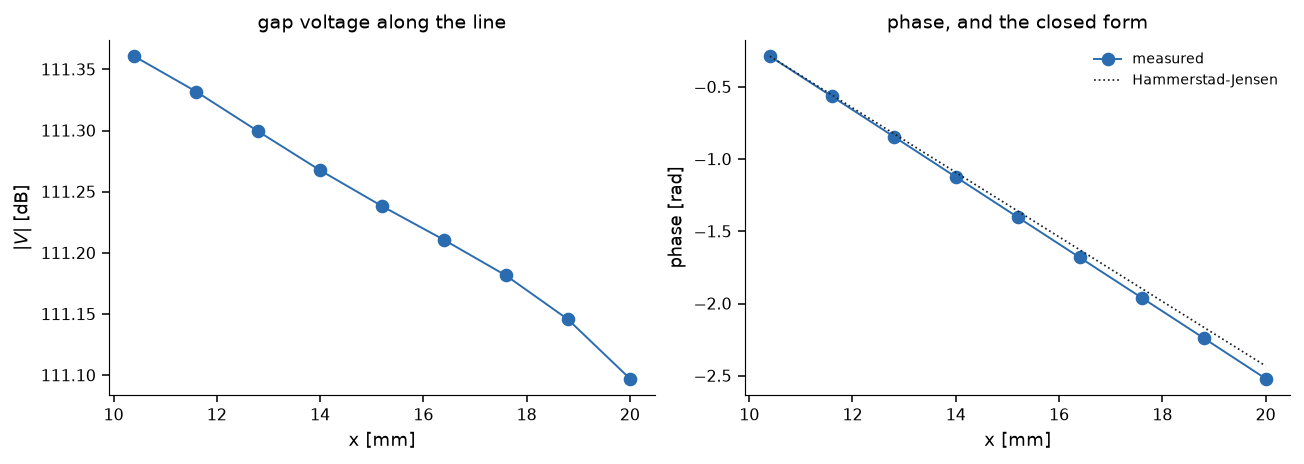
\includegraphics[width=0.92\textwidth]{../figures/ms-line-phasors.png}
  \caption{The record the estimators are fitted to. Left: $|V|$ in decibels at the nine station planes against
  $x$ in millimetres. Right: the unwrapped phase in radians against $x$, with the closed-form
  Hammerstad--Jensen ramp dotted beside it -- the closed form is a straight line of the slope the model predicts,
  not a fit to the points. The envelope falls by $3.0$ per cent across the span while each half fit is good to
  $1.4\times10^{-3}$; the ripple riding on that fall is the standing wave of
  Section~\ref{sec:msres-verdict}, and it is why a single exponential through these points absorbs a bias.}
  \label{fig:ms-phasors}
\end{figure}

\begin{figure}[H]
  \centering
  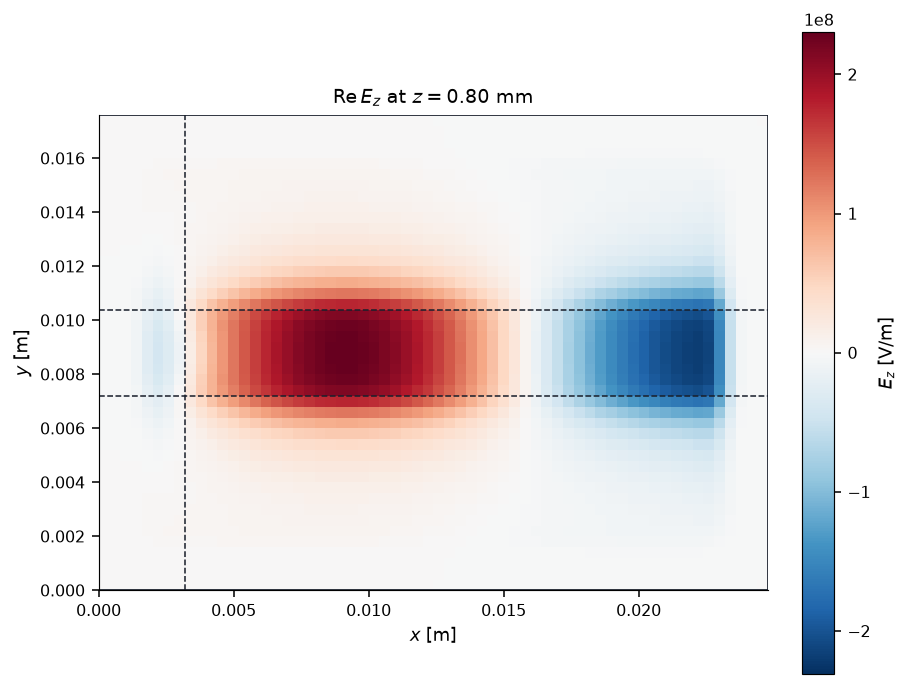
\includegraphics[width=0.62\textwidth]{../figures/ms-midplane-ez.png}
  \caption{Real part of the $5.8278$ GHz phasor of $E_z$ in volts per metre, on the node layer halfway up the
  $1.60$ mm substrate ($z = 0.80$ mm at the reference box's cell size), taken as the mean of the two cells that
  straddle that layer. The phasors are complex and a colour map is not, so the real part is what is drawn: this is
  the field at the phase the accumulated record starts on, not an amplitude. Dashed: the port plane and the two
  strip edges. The fringes along the line are the forward wave beating with the backward one, whose coefficient
  this record puts at $|\gamma| = 0.0063$; an amplitude plot would show a monotone taper and none of them.}
  \label{fig:ms-midplane}
\end{figure}

The two figures are the record itself rather than a summary of it, and they are worth reading against the tables
in one respect only: the phase panel's slope and the magnitude panel's fall are the two quantities
Table~\ref{tab:ms-alpha} disagrees with itself about, and both are visible by eye. What they do not show, and
what the accounting table does, is where the power went -- a picture of the line cannot distinguish a mode that
decayed in place from one that lost power to the lateral walls, because both look like a falling envelope on the
axis the stations sit on.
 % \section{The reference box: what one line actually measures}
\section{Measuring a number you can defend}
\label{sec:method}

\noindent\emph{Status: draft -- this section is an argument, not a result. Nothing in it is computed. It is the
rule that the measurements of this report are held to, written after breaking that rule at least once each.
Every number used as an example is the report's own, and the section it came from is cited so that the reader
can check the break rather than take my word for the correction.}

Every number in this report arrived by the same three-step route. A field was stepped, a record was written to
disk, and somebody applied an arithmetic operation to that record and called the result a measurement. The
arithmetic is not the problem: dividing two fluxes, taking a logarithm, fitting an exponential, and inverting a
$2\times 2$ system are all legitimate operations, and all of them appear in what follows. The problem is the
noun. \emph{Measurement} carries an implicit claim of independence, and most of the numbers in this report
cannot support that claim: they are derived quantities, and a derived quantity inherits every assumption of the
derivation while looking, in a table, exactly like something that was observed. What follows is the audit of
that word, in the order in which the mistakes were made. It is written in the first person because the errors
are mine, and it is written as a list of rules because a rule can be seen to be broken, while a good intention
cannot.

\subsection{A number without provenance is not a number}
\label{sec:method-provenance}

Before the rules about derivation, there is a rule about the record itself. A number in this report is a
statement about a particular run of a particular mesh processed by a particular estimator, and unless all three
are named the number is not reproducible even in principle. Two runs of the same structure at the same mesh
differ in their truncation of the field outside the computational window, in the frequency they were driven at,
and in the length of the record that was transformed; two estimators applied to one run differ far more than
that, as the next subsection shows. A single printed value is therefore a summary of a triple, and a value whose
triple has been lost is a rumour.

This is why Section~\ref{sec:worked} is built around a four-column table whose middle two columns are the
provenance: the cell size and the mesh counts, the estimator, the record length and the drive frequency. It reads
as bureaucracy and it is the only part of that table which cannot be argued with. Where the provenance is
missing, the number is marked as such rather than reconstructed, because reconstructing it means choosing the
run that makes it most plausible, which is a way of fitting the provenance to the answer.

The most useful thing provenance does is to make a class of disagreement impossible. When two numbers in the
record do not match -- and several do not -- there are two separate questions: could these two numbers have come
from the same run, and do they in fact agree. These are routinely conflated, and I conflated them myself. A
published pairing of $|S_{11}|$ and $|S_{21}|$ once recorded a $7.3$ per cent passivity deficit, while the single
record that now carries both quantities gives $|s_{21}|^2 + |\gamma|^2 = 0.96228$, a $3.77$ per cent deficit at
the same frequency. My first note on the discrepancy claimed that the pairing \emph{could not} have come from a
single run. That claim was too strong and it was wrong: a single run does yield both numbers at the resonance,
and they are simply different numbers. The failure is a numeric mismatch, which is a fact about the record, and
not a provenance impossibility, which would have been a fact about the archive.

The distinction matters because the two failures have different remedies. A provenance impossibility is closed
by finding the missing run; a numeric mismatch is closed only by re-measuring, and until then it is reported as
an open discrepancy. Saying the strong thing when the weak thing is true is not caution. It is a second error,
committed in the direction of looking rigorous.

\subsection{A fit is not a measurement}
\label{sec:method-fit}

The first rule is the one I broke most often, and the one that is easiest to break without noticing, because
fitting feels like measuring. You take a record, you choose a model, and the model returns a number with a
residual beside it; the residual looks like an error bar, the number looks like a result, and the fact that the
model \emph{was} the source of the number is invisible in the output.

It is not invisible in the logic. If a quantity is extracted by fitting a model to a record, then that quantity
is a property of the pair (record, model), not of the record alone. Change the model and the number changes; the
only defence is that the model be forced by something outside the record, and that its misfit be reported rather
than absorbed. A quantity recovered by fitting is therefore not an independent measurement of anything. It is a
projection of the record onto a chosen family of curves, and it can be perfectly repeatable, perfectly smooth in
the fit parameter, and wrong by a factor.

The clearest instance in this report is the attenuation of the microstrip line, where two different models of
the same record return rates that differ by a factor of $1.86$: the two-wave fit returns about
$0.0215$\,dB/mm against an audited $0.0116$\,dB/mm for the work the walls actually removed
(Section~\ref{sec:msres-alpha}). Both fits converge; neither reports a large residual; the fit is simply
describing a record that does not contain what the model says it contains. The audited figure is not a fit at
all -- it is a volume integral of $\sigma|\mathbf{E}|^2$ over the conductors, divided by the power entering the
section -- and that is why it is the one that is quoted, and why the fit is quoted only as a fit.

The same rule applies one level down, to quantities that are definitionally tied to the fitted ones. The
effective permittivity of Section~\ref{sec:tline-epseff} is $\eps_{\mathrm{eff}} \equiv (\beta c/\omega)^2$: once
$\beta$ is known, $\eps_{\mathrm{eff}}$ adds no information whatsoever and inherits the full uncertainty of the
fit that produced $\beta$. Reporting both is legitimate bookkeeping. Reporting both as \emph{two} numbers, or
worse, as agreement between two numbers, is a category error, because the second cannot disagree with the first.
This is why Section~\ref{sec:worked} lists $\eps_{\mathrm{eff}}$ as a restatement of the phase constant rather
than as a second result, and why the fit residual of that record, $0.0128$, is recorded as a property of the fit
and never used as an error bar on anything.

\subsection{Never use the quantity under test as its own oracle}
\label{sec:method-oracle}

A special case of the first rule deserves its own heading, because it survives review: an estimator can be
built out of the very assumption it is supposed to test. If you estimate transmission by assuming the field
envelope is constant, then your estimator has already asserted the result. It cannot detect a departure from a
constant envelope, because the departure is the thing the model was built to ignore. The estimator is not
biased in the statistical sense, where more data would eventually correct it; it is blind, and more data
sharpens the blindness.

This is what happened to the flux estimator that was for a while the report's headline measurement of loss. The
field was sampled at nine stations along the line, the time-averaged Poynting flux was formed at each, and the
square root of the last divided by the first was read as a transmission coefficient. On paper that is a
model-free measurement of attenuation. In fact the estimator assumes that the flux at a station is a smooth
function of position, declining because energy is being absorbed -- that is, it assumes what it is measuring.
Where the assumption holds it returns a plausible number; where it fails it returns a number of the same
plausible size, because the failure mode, a standing wave, is itself a smooth function of position. There is no
residual to warn you. Section~\ref{sec:worked} takes this record apart station by station and shows the reading
was dominated by a standing-wave ripple in the flux, not by absorption.

The same trap sits in every de-embedding step. Moving a reference plane by $d$ assumes a single travelling wave
of known $\beta$; if a reflected wave is also present, the move mixes them, and the mixing is smooth and
plausible. The rule that follows is blunt: before trusting a derived number, ask what the derivation assumed,
and then ask whether that assumption is precisely the proposition the number is supposed to establish. If it
is, the number is decoration.

\subsection{Stability is not accuracy}
\label{sec:method-stability}

A ratio is the most reassuring object in numerical work, because it cancels. Systematic errors that scale both
numerator and denominator leave the ratio untouched, and a ratio that moves by a part in a thousand between runs
feels like a measurement accurate to a part in a thousand. That feeling is wrong whenever the thing that is
stable is the \emph{scale} rather than the \emph{shape}.

Take two numbers that are both short by the same factor: $a \to \alpha a$ and $b \to \alpha b$. Their ratio
$a/b$ is unchanged, exactly, and remains unchanged as $\alpha$ wanders over any range at all. The ratio is
perfectly stable and completely silent about $\alpha$. Every quantity in this report that is extracted as a
ratio is exposed to this: the reference impedance from the ratio of the two modal voltages, the transmission
coefficient from the ratio of two fluxes, the reflection coefficient from the ratio of two sampled amplitudes.
If a common gain error, a common cell-volume convention, or a common windowing factor sits on both terms of the
ratio, then the ratio is reproducible to many digits while the absolute level is wrong by tens of per cent.

The way to tell the two apart is to break the commonality deliberately. If the numerator and denominator are
computed by genuinely different operations -- a volume integral of dissipation on one side, a flux integral over
a surface on the other -- then a common factor is unlikely and the ratio means something. Where both terms come
from the same field dump through the same windowing and the same normalisation, the ratio measures the
arithmetic and not the physics. That test is what separates the audited attenuation of
Section~\ref{sec:ms-accounting} from the station ratios of Section~\ref{sec:ms-estimators}: the audit divides
joules lost by joules entering, computed from different parts of the field, while the station ratio divides two
samples of the same quantity taken by the same operation. The first is a measurement that happens to be a
ratio; the second is a ratio that is not a measurement.

\subsection{A tolerance needs a pair of measurements}
\label{sec:method-tolerance}

A single number has no error bar. It has a value, and the value is exact in the sense that it was printed, and
nothing about it says how far it might sit from the truth. A target with no error bar therefore cannot be
failed: the comparison of one number against a bound is a comparison of two conventions, and the convention
wins or loses by fiat rather than by evidence.

This is not a philosophical point, it is the reason the acceptance criteria of this report are written the way
they are. When the criterion of Section~\ref{sec:ms-criterion} asks whether a measured rate of loss sits within
a stated band, it can only do so because there are two independent routes to the rate -- the audited joule
budget and the fitted decay -- whose \emph{difference} is a quantity with a meaning. The difference can be
large or small; that is evidence. One number compared against a target is not evidence of anything, and a
document full of such comparisons is a document that has never been tested.

The failure is common enough in this report's own history to be embarrassing. The reflection result of
Section~\ref{sec:msres-verdict} was for a while quoted as ``$-44.48$\,dB, goal $-20$\,dB met with $24$\,dB to
spare''. That is a true sentence and it is not a measurement, because the $24$\,dB is a statement about a
tolerance chosen in advance, not about the difference between two ways of obtaining the reflection. The moment a
second route was computed -- the summary line of the same dump carrying $|\gamma| = 0.00628$ against the
$0.00597$ of the plane rows, $5.2$ per cent apart -- the number acquired a real error bar, and the honest
statement became that the agreement is good to a few per cent and that the $5.2$ per cent itself is
unreconciled. Both statements describe the same run. Only the second one can be wrong.

The corollary is that a report which states tolerances must state them twice: once as the band it wishes to
meet, and once as the spread of the routes it actually has. Where there is only one route, the second number is
absent and the tolerance should be described as advisory, not met.

\subsection{Transients get a discard window, not a correction}
\label{sec:method-transients}

Every time-domain record begins before the physics does. The drive is switched on into a structure that is not
yet in its steady state, energy has not yet filled the section, and the reference plane sees a field that
contains the switch-on as well as the wave. There are two ways to deal with this, and only one of them is
honest.

The honest way is to discard. Accumulate the transform over a window that begins after the transient has left
the domain of interest, and report the start of the window as part of the provenance of the number; if the
window cannot be made long enough for the residual transient to be negligible, the number is provisional, not
corrected. The dishonest way is to model the transient -- to fit a decaying offset, subtract a mean, or
otherwise take the switch-on out of the record -- because the model of the transient is a hypothesis about the
same structure whose behaviour you are trying to measure. The correction and the measurement then share a
model, and the first rule applies again.

The record used throughout this report discards the first $600$ of $2400$ steps and accumulates over the
remaining $1800$, and that choice is stated with the number rather than buried in a script, because it is part
of what the number means. The window is not a convenience: a record that begins at step zero contains a
transient of the order of the resonator's filling time, and a transform over the whole record would mix it in.
Nothing about the arithmetic afterwards can remove it, so nothing is attempted; the window is the whole of the
treatment.

The same logic governs the drive. A resonant record is only as good as the frequency it was driven at, and the
report's records are driven at a snapped frequency that differs from the requested one by $-13.3$ parts per
million. That offset is small, and it is quoted anyway, because a resonance measured at a frequency that is not
the one you asked for is a resonance of a slightly different structure, and the reader is entitled to know how
different. Correcting the result to the requested frequency would require the very dispersion model that the
result is supposed to test.

\subsection{A repeatable diagnostic is still a diagnostic}
\label{sec:method-diagnostic}

The last rule is the one this report needed longest to learn, and it concerns a class of quantity that is
\emph{perfectly} well behaved. A diagnostic quantity is one that is computed by a clean operation from a clean
record, returns the same value every time the record is reprocessed, varies smoothly with the run parameters,
and is entirely useless for the purpose its name suggests. Its repeatability is what makes it dangerous: a
quantity that scattered would be caught immediately, whereas a quantity that is stable to five digits looks
like the best number in the document.

The station-profile tilt of Section~\ref{sec:worked} is such a quantity. It is the fractional change in the
time-averaged Poynting flux between the first and last station of a nine-point array, it is trivially
reproducible, and it was for a period quoted as a transmission coefficient and hence as a rate of loss. It is
not a rate of loss. The stations span about a third of a guide wavelength, so the standing wave that exists on any
real line -- including a lossless one -- is not averaged over the span at all; what the tilt measures is the
phase at which the array happens to be sampled. The reading is stable because the sampling is deterministic, not
because the physics is captured. Its correctness as an arithmetic average is not in question; its competence as
a measurement of attenuation is nil, and no amount of repetition can change that.

The rule that follows is a naming rule. A quantity may be reported as a diagnostic, with the word in its label
and the caveat in its paragraph, or it may be reported as a measurement. It may not be reported as a
measurement because it is stable, because it is convenient, or because it agrees with something else. And if a
later audit shows that a quantity which was published under a measurement name in fact measures a sampling
artefact, the correct response is to relabel it and keep the value -- the value is a fact about the record and
should not be destroyed -- while withdrawing every conclusion that leaned on the name. That is the procedure
applied to the tilt in Section~\ref{sec:worked}, and to the two ``field loss'' figures that preceded it, both of
which are withdrawn in favour of the audit that replaced them.

\subsection{What it cost, and what it bought}
\label{sec:method-cost}

The rules above are cheap to state and were expensive to learn. The price of getting them wrong is not an error
bar on one number; it is a whole chain of reasoning built on a noun. A derived quantity that is called a rate of
loss will be compared against an audited rate of loss, will agree with it to a couple of per cent, and the
agreement will be written down as independent confirmation -- when in fact the two are the same arithmetic on
the same field, and the agreement is a coincidence or an identity. Withdrawing the second as a witness leaves
the first standing, which is the correct outcome, but it also removes a paragraph of the argument, and the
paragraph has to be rewritten rather than deleted.

Section~\ref{sec:worked} is the ledger of that process for four numbers, with the status of each recorded as
quotable, diagnostic only, or withdrawn. It is deliberately unflattering. The report has a much smaller number
of real measurements than its length suggests, and after the audit they are: cavity frequencies against an
analytic spectrum, a reflection coefficient against a matched reference plane, an attenuation against a joule
audit, and a scattering width against a Mie series -- each of them a comparison of two independent routes to one
quantity, which is the only shape in which a number can be defended. Everything else in this document is either
a restatement of one of these, a diagnostic that is named as one, or arithmetic that would fail the tests above
if it were called a measurement. That is not a comfortable inventory for a document of this size. It is,
however, an inventory that can be checked, and a number that can be checked is worth ten that cannot.
     % \section{Measuring a number you can defend}
\section{Four numbers, and what happened to them}
\label{sec:worked}

\noindent\emph{Status: draft -- a ledger, not a result. The four quantities below have all been quoted in this
report at some time, and they are now sorted by whether they can still be quoted. Two of them cannot, one only
after being renamed, and one can with a caveat attached to its reference impedance. The values are printed here
exactly as the records give them; the sorting is the content. The rules applied are those of
Section~\ref{sec:method}.}

A measurement that is withdrawn is more useful than a measurement that is quietly repaired. When a number stops
being defensible, the temptation is to adjust it -- to change the normalisation, to choose a longer window, to
report the value from the run that agrees -- and to keep the sentence it supported. Doing so destroys the only
evidence that the earlier reasoning was wrong, and it hides the cost. This section therefore keeps every value
and changes only the status word beside it: a number may be quotable, diagnostic, or withdrawn, and the value is
never the thing that is corrected. In two of the four cases below the status moved a long way while the digits
did not move at all, and that is exactly the outcome this ledger exists to display.

\subsection{The ledger}
\label{sec:worked-ledger}

\begin{table}[H]
  \centering
  \caption{Four quantities from this report's records, with provenance and the status they now carry.
  \emph{Quotable}: the record supports the quantity as a measurement of what its name says. \emph{Diagnostic
  only}: the quantity is exact and repeatable, but it measures a property of the sampling rather than of the
  device, and is reported under a name that says so. \emph{Withdrawn}: the quantity was quoted as a measurement
  and is not one; the value is retained for the audit trail and must not be cited. The provenance column is
  part of the number: a value whose run, mesh and estimator are not stated here is not reproducible.}
  \label{tab:worked}
  \small
  \begin{tabular}{@{}p{3.1cm}p{3.2cm}p{6.2cm}p{2.0cm}@{}}
    \toprule
    Quantity & Value & Provenance: run, mesh, estimator & Status \\
    \midrule
    (a) Transmission coefficient, phase constant and reference impedance of the reference box at
    \SI{5.8278}{\giga\hertz}
    & $s_{21} = 0.98088 + 0.00476\,j$;\newline $\gamma = 0.01022 + 0.00418\,j$;\newline
      $z_0 = 49.76 + 13.59\,j$\,\si{\ohm};\newline $\beta = 229.554$\,m$^{-1}$
    & CW run, mesh $132\times104\times38$ with a \SI{0.2}{mm} cell; driven at \SI{5.827786408327}{\giga\hertz}
      against a requested \SI{5.827864}{\giga\hertz}; $600$ of $2400$ steps discarded, $1800$ accumulated over
      $6.8636695303115883\times10^{-10}$\,s; two-wave fit at a transverse cut
    & quotable \\
    \addlinespace
    (b) Station-profile tilt of the time-averaged Poynting flux
    & $0.987038$ as a ratio;\newline $6.48$ per cent as a tilt
    & CW run at \SI{5.8278}{\giga\hertz}; nine stations at cells $52$--$100$ of the propagation axis, \SI{9.6}{mm}
      span; flux formed by time-averaging $\mathbf{E}\times\mathbf{H}$ at each station, then
      $r = \sqrt{s_9/s_1}$
    & diagnostic only \\
    \addlinespace
    (c) ``Field loss'' of the reference box
    & $16$ per cent, later ``at most'' $2$ per cent
    & the same nine-station arrays as (b), read through two different normalisations; no separate run exists
    & withdrawn \\
    \addlinespace
    (d) Passivity deficit from a paired $|S_{11}|$ and $|S_{21}|$
    & $7.33$ per cent
    & its provenance is not established in this report
    & withdrawn, pending \\
    \bottomrule
  \end{tabular}
\end{table}

Three of the four rows are the same record, and that is the point of the table rather than a defect in it. One
field dump was processed four ways: a two-wave fit at a cut, a nine-station flux profile, a loss figure derived
from that profile, and -- in the fourth row -- an unrelated published pair that turned out not to reproduce. The
first is quotable, the second is a diagnostic, the third is withdrawn, and the fourth is withdrawn pending. The
digits in rows (a) and (b) have not changed since they were first written down. Only the claims attached to them
have, and the next three subsections say why for each.

A status is assigned by three tests, and they are mechanical enough to be checked by a reader. First, does the
derivation of the quantity assume the proposition the quantity is supposed to establish? A flux ratio that
assumes a smooth envelope fails this test whatever its value. Second, is the quantity a ratio of two numbers
obtained by the same operation on the same field dump? If so it may be stable to many digits and still say
nothing about level, and it cannot be quotable on its own. Third, does the record carry a second, independent
route to the same quantity? Only where all three tests pass does the word quotable apply, and the tests are
applied to the quantity as it is used in a sentence, not to the quantity as it might in principle be computed.
Row (b) is an exact number and fails the first test; rows (c) and (d) fail it outright; row (a) passes all
three, which is why it is the only row that is quotable.

\subsection{Quotable: one controlled transmission record}
\label{sec:worked-cw}

The record of row (a) is the best-controlled run in the report, and it is quotable because every assumption in
its reduction was checked against something else in the same record. The mesh is $132\times104\times38$ cells
with a \SI{0.2}{mm} cell, which puts the transverse cross-section at roughly a tenth of a guide wavelength; the
drive was snapped to the nearest frequency the discrete time step can represent on the transform grid, which is
\SI{5.827786408327}{\giga\hertz} against a requested \SI{5.827864}{\giga\hertz}, an offset of
$-77\,591.67$\,Hz, or $-13.3$\,ppm; the step is $\dd t = 3.8131497390619936\times10^{-13}$\,s; and the first
$600$ of $2400$ steps were discarded, leaving $1800$ accumulated steps spanning $6.8636695303115883\times10^{-10}$\,s.
The offset of $-13.3$\,ppm is quoted rather than absorbed because it is a property of the drive: a resonance
measured $-13.3$\,ppm away from the requested frequency is the resonance of a slightly different structure,
and the reader is entitled to know by how much.

At that drive the two-wave fit at a transverse cut returns
\begin{equation}
  \begin{aligned}
    s_{21} &= 0.9808843848072781 + 0.004761855437949522\,j , \\
    \gamma &= 0.010215720318428398 + 0.004178365747705708\,j ,
  \end{aligned}
  \label{eq:worked-s21}
\end{equation}
with $|\gamma| = 0.0110371953841$ and a fit residual of $0.0128478440321$. The reflection coefficient is the
reason this record is quotable and the others are not: at $|\gamma| \approx 0.011$ the standing-wave ratio on
the line is $1.022$, so the field at a cut is very nearly a single travelling wave, and the two-wave model is
forced by the record rather than imposed on it. In the records of Section~\ref{sec:msres-alpha} the same model
returns a rate that disagrees with the joule audit by a factor of $1.86$; here there is no fitted rate at all,
only a complex amplitude at a cut, and the quantity being quoted is that amplitude.

Two numbers in the same reduction need their status stated separately, because both look like measurements and
only one is. The effective permittivity is $\eps_{\mathrm{eff}} = 3.53220159465$, and it is a restatement of the
phase constant: by $\eps_{\mathrm{eff}} \equiv (\beta c/\omega)^2$, once $\beta = 229.554353095$\,m$^{-1}$ is
known at a known $\omega$ the permittivity is arithmetic, and it cannot disagree with the phase constant by so
much as a digit. It is recorded because a reader wants it and because the dispersion curves of
Section~\ref{sec:dispersion} are drawn against it; it is not a second measurement of anything, and any sentence
of the form ``the phase constant and the effective permittivity agree'' would be a sentence about a
substitution.

The reference impedance is the number with the caveat. The fit returns
\begin{equation}
  z_0 = 49.76097429242066 + 13.592389198926165\,j \,\si{\ohm} ,
  \qquad |z_0| = \SI{51.5839859517}{\ohm} \text{ at } 15.277852^{\circ} ,
  \label{eq:worked-z0}
\end{equation}
and the imaginary part is not noise. An imaginary term of \SI{13.6}{\ohm} in the reference impedance says that
the line cannot be referred to a real \SI{50}{\ohm} reference without a transformation: the reflection
coefficient, and therefore every $S$-parameter computed from this record, depends on which reference impedance
is assumed, and ``the transmission coefficient of this line'' is not a well-defined number until the reference is
named. That is not a defect of the fit and it is not a large effect -- the angle is $15^{\circ}$, so
$\operatorname{Re} z_0$ is within a per cent of \SI{50}{\ohm} -- but it is the kind of caveat that has to travel
with the number rather than be rediscovered by whoever uses it next. Accordingly the quotable claim is the pair
of amplitudes of equation~\eqref{eq:worked-s21} together with the reference of
equation~\eqref{eq:worked-z0}, and any statement of an attenuation or a mismatch derived from them is only as
good as the reference it was derived against.

The record also carries its own conservation check, and it is this rather than the smallness of $|\gamma|$ that
lets the third test of Section~\ref{sec:worked-ledger} be passed. From the amplitudes of
 equation~\eqref{eq:worked-s21},
\begin{equation}
  |s_{21}|^{2} + |\gamma|^{2} \;=\; 0.96228 ,
  \label{eq:worked-cw-passivity}
\end{equation}
so $3.77$ per cent of the incident power is neither returned nor transmitted and is accounted for as absorbed in
the section. That is not a second measurement of the transmission coefficient -- it is the same two amplitudes
entered once more -- but it is an independent check on the \emph{pair}, because passivity is a property of the
structure and not of the fit: a fit that returned a transmission above unity, or a reflection inconsistent with
the standing-wave ratio at the cut, would fail here even if each amplitude separately looked plausible. It is
also the number that the pairing of Section~\ref{sec:worked-pairing} fails to reproduce, which is why the two
rows are worth reading side by side: one record, two amplitudes, and a deficit of $3.77$ per cent on one line of
arithmetic, against a published $7.33$ per cent that cannot be recovered from it.

\subsection{Diagnostic only: the station-profile tilt}
\label{sec:worked-tilt}

The second number is the one this section exists for, because it is the only number in the report that was
demoted without any digit changing, and because the demotion was forced by an identity rather than by a
disagreement.

The construction is this. The field is sampled at nine stations spaced six cells apart along the propagation
axis, \SI{1.2}{mm} apart, spanning \SI{9.6}{mm}. At each station $k$ the time-averaged Poynting flux $s_k$ is
formed by averaging $\mathbf{E}\times\mathbf{H}$ over the accumulated window, and the flux at the last station is
divided by the flux at the first to give a transmission-like ratio $r = \sqrt{s_9/s_1}$. If the flux declined
only by absorption, then $r = |S_{21}|$ and the record measures attenuation. The reason it does not is that the
two quantities $r$ and the fractional drop of the flux are related by an identity in which the attenuation does
not appear at all.

Let $\tau$ be the tilt of the station profile, the drop from first to last measured against the mean of the
array, and $\bar{s}$ that mean. Then
\begin{equation}
  1 - r^{2} \;=\; \frac{s_1 - s_9}{s_1} \;=\; \tau \cdot \frac{\bar{s}}{s_1} ,
  \qquad
  \tau \;=\; \frac{s_1 - s_9}{\bar{s}} .
  \label{eq:worked-tilt}
\end{equation}
Nothing in equation~\eqref{eq:worked-tilt} refers to a material, a cross-section or a rate. It is an algebraic
relation between three averages of the same nine numbers, and it says that whatever $r$ reports, it reports a
property of the shape of the station profile, scaled by the ratio of the mean to the first value. If the profile
declines linearly, $\bar{s}/s_1$ is close to one and $1 - r^2$ is nearly the tilt; if the profile is a standing
wave sampled at an arbitrary phase, the same is still true, and the number that comes out is the amplitude of
the standing wave, not the loss.

The CW record at \SI{5.8278}{\giga\hertz} gives, at the nine stations lying on cells
$52$, $58$, $64$, $70$, $76$, $82$, $88$, $94$ and $100$,
\begin{equation*}
  \begin{aligned}
    s_1, \dots, s_9 \;=\; {} & 6614.038753,\ 6584.568766,\ 6563.085584, \\
    & 6543.527531,\ 6516.123028,\ 6470.735308, \\
    & 6400.792767,\ 6306.335991,\ 6194.943464 ,
  \end{aligned}
\end{equation*}
with a mean of $6466.0168$. The last station over the first is $s_9/s_1 = 6194.943464/6614.038753 = 0.936635$, a
power ratio, so the power deficit is $6.3365$ per cent, printed as $6.34$. The amplitude transmission is its
square root, $r = \sqrt{s_9/s_1} = 0.96780$, and a deficit taken on that basis is $3.22$ per cent. On the same
array the tilt is $6.4815$ per cent and the mean-to-first factor is $0.977617$, and their product,
$6.4815 \times 0.977617 = 6.3364$ per cent, against the measured $6.3365$ per cent: a residue of $0.0001$
per cent, the size of rounding the tilt to four decimal places, so the product reproduces the power deficit
at the quoted precision and not to the last printed place. That agreement is not a coincidence to be
explained; it is equation~\eqref{eq:worked-tilt} holding, as it must, because the three numbers are three
averages of one array. The reason the deficit and the
tilt are so close is that the profile is nearly straight over nine points, which is what a fraction of a
standing-wave period looks like.

A deficit quoted as a bare percentage is therefore ambiguous until it says whether the ratio it came from was a
power ratio or an amplitude ratio. Here the two differ by close to a factor of two: $6.34$ per cent on the power
ratio $0.936635$, $3.22$ per cent on the amplitude ratio $0.96780$. That is one way a number acquires two
defensible-looking values, and it is why this report prints the ratio as well as the percentage.

The same extraction on the pulse record at \SI{5.333}{\giga\hertz} gives a deficit of $1.9561$ per cent against a
tilt of $1.9757$ per cent and a mean-to-first factor of $0.9901$; the product is $1.9561$ per cent, and there the
identity closes to every printed digit. On the substrate-only record the nine stations are
\begin{equation*}
  \begin{aligned}
    s_1, \dots, s_9 \;=\; {} & 4879.172642,\ 4867.110209,\ 4862.878825, \\
    & 4859.305586,\ 4847.939993,\ 4820.684887, \\
    & 4772.478055,\ 4703.721293,\ 4621.547925 ,
  \end{aligned}
\end{equation*}
with a mean of $4803.871$, a ratio of $0.97324$ ($5.27$ per cent), a tilt of $5.363$ per cent and a
mean-to-first factor of $0.984568$, whose product is $5.28$ per cent. Three records, three arrays, and in every
one the ``attenuation'' is the tilt multiplied by a factor within a few per cent of one.

That is the whole of the diagnostic, and the geometry says why it is a diagnostic. The stations span
\SI{9.6}{mm}. At \SI{5.8278}{\giga\hertz} the free-space wavelength is \SI{51.449}{mm}, and with the
$\eps_{\mathrm{eff}} = 3.5322$ of the controlled record of Section~\ref{sec:worked-cw} the guide wavelength of
the cross-section they sample is $\lambda_g = \lambda_0/\sqrt{\eps_{\mathrm{eff}}} =
\SI{51.449}{mm}/1.879415 = \SI{27.375}{mm}$, so the span is $0.35\,\lambda_g$. The flux on a line carrying a
forward and a reflected wave ripples at twice the phase constant, that is, with period
$\lambda_g/2 = \SI{13.688}{mm}$ in space, so the array covers seventy per cent of one period of that ripple. The
first and last stations of such a sample can fall at \emph{any} relative phase, including the phase that makes
them differ by several per cent while the line is lossless, and seven tenths of a period is nowhere near enough
of the ripple to average it out. A reading that does not average the standing wave is confounded at any loss
level, including zero.

What that reading was called is the history this subsection records. The quantity was for a period written as
$|S_{21}|_{\text{poynting}} = 0.987038$ and quoted as an attenuation of $-0.1133$\,dB over the \SI{9.60}{mm}
span, which is the largest single contribution the report ever claimed towards the loss of the reference box,
and it was presented as model-free -- which, in the sense of ``containing no fitted parameter'', it was. It is
now called the station-profile tilt, and it carries \emph{no} attenuation claim. The value $0.987038$ survives
in the table and in this sentence; the name does not, because the name is what the arithmetic does not support.
The correspondence is exact: $20\log_{10}(0.987038) = -0.1133$\,dB, so nothing has been recomputed, only
relabelled, which is the honest form of a correction.

Two further consequences follow from the relabelling, and both were visible only afterwards. The first is that
the tilt cannot serve as a bound on the loss either. At resonance, the full-section tilt of $6.48$ per cent is
larger than the circuit-level passivity deficit of $3.77$ per cent computed from the amplitudes of
equation~\eqref{eq:worked-s21}; a quantity that exceeds the thing it is supposed to bound is not a bound, it is
a different quantity. On the substrate-only record the tilt is $5.36$ per cent against the same $3.77$ per cent,
and there it does bound the deficit -- which is the one surviving quantitative role of the construction, and the
reason it is a diagnostic worth keeping rather than deleting. The second consequence is that the tilt is a good
measurement of something else, namely of how much standing wave is present at the array: a tilt far above the
passivity deficit is evidence that the sampling sits inside a ripple, which is exactly the warning one wants
before quoting any between-station rate. The array was doing useful work all along. It was just not doing the
work it was named for.

\subsection{Withdrawn: the field-loss figures}
\label{sec:worked-withdrawn}

Two published figures are withdrawn outright: a ``$16$ per cent field loss'' of the reference box, and, before
that, a figure of ``at most $2$ per cent''. Both were computed from the nine-station arrays of
Section~\ref{sec:worked-tilt}, through two different normalisations of the same flux profile, and both are
therefore readings of the tilt rather than of a loss.

The withdrawal is not a small correction and it is worth saying plainly what it removes. Between ``at most $2$
per cent'' and ``$16$ per cent'' lies a factor of eight, and both numbers were at some point the report's answer
to the question of how much the reference box loses. They differ because the two normalisations respond
differently to where the standing wave sits in the array -- which is the signature of a sampling artefact and not
of physics, since a physical loss cannot change by a factor of eight when nothing about the geometry changes.
The audit of Section~\ref{sec:worked-tilt} explains both figures with one mechanism, arithmetic on nine
numbers, and that explanation is the reason they are withdrawn rather than demoted. A diagnostic is a quantity
that is exactly what it is; these two were never exactly anything, because the normalisation was chosen after
the fact to make the number plausible.

What replaces them is not another reading of the same array. The rate of loss that the report now quotes for the
reference box comes from the joule audit of Section~\ref{sec:ms-accounting}, in which the power dissipated in
the conductors is integrated over the volume of the metal and divided by the power entering the section, and it
is $0.01160$\,dB/mm. That number is not a ratio of two samples of the same quantity and it does not depend on
where the standing wave sits; it is the work the walls actually did. The station arrays remain, and their tilt
remains, as the audit trail for the withdrawal -- and as a warning attached to any future flux-based reading:
nine stations spanning a third of a guide wavelength cannot measure a loss, whatever they are called.

\subsection{Withdrawn pending: the passivity pairing}
\label{sec:worked-pairing}

The fourth row is different from the other three in every respect: it comes from a different reduction, it does
not involve the station arrays, and it is withdrawn pending a question that has not been answered rather than
withdrawn because the answer is known.

A published pairing of $|S_{11}|$ and $|S_{21}|$ at the reference box recorded a passivity deficit of $7.33$ per
cent, that is, $|S_{11}|^2 + |S_{21}|^2$ short of unity by that fraction at resonance. A single CW record now
carries both coefficients at the same frequency, and it gives
\begin{equation}
  |s_{21}|^{2} + |\gamma|^{2} \;=\; 0.96228 ,
  \label{eq:worked-passivity}
\end{equation}
a deficit of $3.77$ per cent. The two deficits do not agree: they differ by a factor close to two, far outside
anything that the per-cent-level uncertainties in either record could explain. The row therefore does not
reproduce, and its status is withdrawn pending -- withdrawn because the number it quotes cannot be defended,
pending because the run that produced it has not been found and the question of what it actually measured is
still open.

The correction to the record concerns not the number but the \emph{reason} I first gave for the mismatch, and it
is recorded here because the reason was quoted and was wrong. My first note on the discrepancy asserted that the
pairing \emph{could not} have come from a single run -- that no one field dump could yield both coefficients at
the resonance, so the pairing must be a mixture of two records. That claim is too strong and it is false. A
single CW run does yield both numbers at $f_0$: $\gamma$ from the two-wave fit at a cut, $s_{21}$ from the same
fit, both referred to the same plane. What the single record shows is not that the pairing is impossible but
that it is different: $3.77$ per cent against $7.33$ per cent.

The difference between the two kinds of failure is the reason the correction matters. A provenance
impossibility would be closed by finding the missing run, and the number would then be either vindicated or
replaced. A numeric mismatch is closed only by re-measuring, and until that is done the honest entry is an open
discrepancy with a stated value. By asserting impossibility I had moved the failure into the category with the
easier remedy, and made the report look more rigorous while making it less true -- the second error described in
Section~\ref{sec:method-provenance}, committed in the same direction as the first. What stands now is the weak
statement: the pairing does not reproduce against the single record, the reason is unknown, and the row stays
withdrawn until it is either located or replaced.

\subsection{What the ledger says}
\label{sec:worked-lessons}

One row of four is quotable without qualification. That is the honest count for this stage of the work, and it is
worth reading against the length of the report: the great majority of the numbers in this document are
restatements, diagnostics or arithmetic, and the four entries above are the ones that were load-bearing enough
to audit.

The audit did not leave the argument where it found it, and this section should not be read as claiming that
nothing was lost. Three things were. The ``two model-free readings agree'' finding of
Section~\ref{sec:ms-criterion} is no longer a finding, because one of the two was the tilt; the coincidence that
the tilt lands $1.9$ per cent from the audited rate is recorded and not counted, and the criterion is now
satisfied on the joule audit alone. The $0.671$ fall of the ratio in Section~\ref{sec:msres-verdict} is quoted
and not read, since the quantity that falls is the tilt. And the claim about where the missing loss goes rests
on the audited work per unit length rather than on a comparison of two readings. Each of these is a weaker
statement than the one it replaced, and each is one that a reader can check.

What the ledger buys is the opposite of what it costs. Rows (a) and (b) are the same record, and after the audit
they can both be used -- one as a measurement, one as a diagnostic -- without either contaminating the other,
because the border between them is written down. The alternative, keeping the tilt under its old name, would have
preserved a paragraph of agreement and would have made every future comparison between the report's loss figures
and the literature an unmarked comparison of unlike things. A number that is defendable is worth a paragraph of
argument, and the four rows of Table~\ref{tab:worked} are the accounting.
     % \section{Four numbers, and what happened to them}
\section{Lumped elements at a transverse cut}
\label{sec:loads}

\noindent\emph{Status: draft -- two element kinds are reported here, a series resistance and a shunt
capacitance, both placed at a transverse cut across the strip of Section~\ref{sec:msres-box}. Every series
figure is evaluated against a load-free run of the same line, and every shunt figure against the capacitance the
mesh was asked to inject. The series branch passes the test it was registered against. The shunt branch does not
pass, and is reported as an envelope that says how far it does get and no further.}

\subsection{What a cut means numerically}
\label{sec:loads-cut}

A \texttt{series\_r} load of value \texttt{inf} is a bare open, and the way it is built has to be stated before
any number is quoted. Nothing is assembled at the load position: the cut annihilates the perfectly conducting
mask on one column of dual edges, so the strip stops there and the two halves of the line are joined by nothing at
all. This is not a simplification of a component the solver cannot discretise. The cut \emph{is} the model, and
the only thing standing between the two halves of the strip is the field of the cut itself.

That field is not negligible. A column of edges whose conductor has been removed carries a capacitance of its own
-- the capacitance of the gap across the strip -- and it carries it whether or not a user asked for one. The bare
open therefore does not present a pure open circuit to the line: it presents that gap capacitance in parallel
with whatever the load was meant to be, and a prediction that treats the cut as an ideal series element is wrong
by that amount. What follows measures the term and finds where it stops being a small correction.

\subsection{The series branch}
\label{sec:loads-series}

Three resistances are cut into the strip at $15.20$ mm and each is measured against a load-free run of the same
line, so that the reference branch carries the cut's capacitance and the load branch differs from it in the load
alone. The board and both of its reference numbers are named in the caption of
Table~\ref{tab:loads-series}, and every figure below is read from that record rather than re-derived.

\begin{table}[H]
  \centering
  \caption{The series branch on the reference board: $0.400$ mm cells, $n_{\mathrm{sub}} = 4$,
  $n_{\mathrm{strip}} = 8$, the cut at $15.20$ mm, $2400$ steps, each resistance evaluated against a load-free
  run of the same line. That run drives at $5.8278$ GHz and gives a station impedance
  $Z_c = 50.547 + 4.025j\ \Ohm$, and the cut's capacitance from the mesh formula
  $C_g = n_{\mathrm{strip}}\eps_0\eps_r\,\dd x = 1.2467\times10^{-13}$ F $= 0.1247$ pF, so that
  $Z_g = 1/(j\omega C_g) = -219.061j\ \Ohm$. The fourth column is the textbook series formula evaluated with that
  $Z_c$; the last is the deviation of the measurement from it. The pre-registered prediction for the
  $100\ \Ohm$ point was a deviation of $7.1$ per cent.}
  \label{tab:loads-series}
  \begin{tabular}{@{}rrrrr@{}}
    \toprule
    $R$ [$\Ohm$] & $|s_{21}|$ measured & $\arg s_{21}$ [$^\circ$] & $2Z_c/(2Z_c+R)$ & deviation [pc] \\
    \midrule
     25 & 0.794825 & $+1.4852$  & 0.802640 & $-0.974$ \\
     50 & 0.673329 & $+4.9999$  & 0.670249 & $+0.460$ \\
    100 & 0.549464 & $+13.0870$ & 0.503909 & $+9.040$ \\
    \bottomrule
  \end{tabular}
\end{table}

The textbook formula holds to under one per cent at $25$ and $50\ \Ohm$, and it fails the $100\ \Ohm$ point by
$9.04$ per cent. That failure was not a surprise found afterwards: the discriminator was registered at three
resistances in advance, and the prediction for the third was a few per cent of deviation from the ideal series
reading. The reason the formula fails is the one Section~\ref{sec:loads-cut} gave: it treats the cut as an ideal
series impedance, whereas the one-cell cut also carries $C_g$, so the load the line actually meets is $R$ in
parallel with $Z_g$.

That reading is testable without appealing to the formula under test, by inverting the measured transmission
coefficient for the impedance the line saw, $Z_l = 2Z_c(1/s_{21} - 1)$, and comparing that impedance with
$R \parallel Z_g$ computed from the geometry alone.

\begin{table}[H]
  \centering
  \caption{The same board and the same three resistances, with the load impedance inverted from the measured
  transmission coefficient and compared with $R$ in parallel with the cut capacitance $Z_g = -219.061j\ \Ohm$ of
  Table~\ref{tab:loads-series}. The columns are, left to right, the commanded $R$, the inverted $Z_l$,
  $R \parallel Z_g$, their difference, its modulus, and the deviation of the measurement from
  $2Z_c/(2Z_c + R \parallel Z_g)$; the largest phase difference against that corrected prediction, over the
  three points, is $0.68^\circ$, and the corrected values themselves are $0.805632$, $0.682260$ and $0.544544$.}
  \label{tab:loads-implied}
  \small
  \begin{tabular}{@{}rrrrrr@{}}
    \toprule
    $R$ [$\Ohm$] & $Z_l$ [$\Ohm$] & $R \parallel Z_g$ [$\Ohm$] & diff. [$\Ohm$] & $|$diff.$|$ [$\Ohm$] & corr. dev. [pc] \\
    \midrule
     25 & $26.3162 - 1.2222j$ & $24.6786 - 2.8164j$ & $+1.6377 + 1.5942j$ & 2.29 & $-1.34$ \\
     50 & $49.5174 - 9.2259j$ & $47.5242 - 10.8472j$ & $+1.9932 + 1.6214j$ & 2.57 & $-1.31$ \\
    100 & $81.4314 - 35.4408j$ & $82.7550 - 37.7771j$ & $-1.3235 + 2.3363j$ & 2.69 & $+0.90$ \\
    \bottomrule
  \end{tabular}
\end{table}

The corrected prediction is within $1.34$ per cent at $25\ \Ohm$, $1.31$ per cent at $50\ \Ohm$ and $0.90$ per
cent at $100\ \Ohm$, against deviations of $0.97$, $0.46$ and $9.04$ per cent for the ideal series formula, and
every phase agrees to within $0.68$ degrees. What is left over is a nearly constant offset rather than a
residual that grows with the load: the real part of the difference in Table~\ref{tab:loads-implied} runs from
$-1.32$ to $+1.99\ \Ohm$ and its imaginary part from $+1.59$ to $+2.34\ \Ohm$ across the three, which is the
signature of a small fixed series term in the cut, not of an error in the capacitance. The capacitance the mesh
formula predicts is therefore confirmed by measurement, and the confirmation is worth as much as the test it was
registered against: at $50\ \Ohm$ the load and the line impedance are nearly equal, so the ideal and corrected
formulas agree there almost exactly, and \emph{a single $50\ \Ohm$ probe would have appeared to confirm the
textbook formula by cancellation}. That is why the discriminator was registered across three resistances and
not one.

One detail of the reference branch is a choice and is declared as one. It takes the attenuation for its
propagation constant from the joint complex-$\gamma$ fit of the station series, $3.0436$ Np/m, and the
normalisation of the ratio is built so that the choice of that attenuation is immaterial to what the ratio
reports.

\subsection{What the reference divides out}
\label{sec:loads-ratio}

The series resistances above were each measured against a load-free run, and the size of that correction is easy
to underestimate: a loaded record cannot be normalised against itself. On the record named in the caption of
Table~\ref{tab:loads-ratio} one loaded run is quoted three ways: with the load-free twin supplied as its reference,
with no reference at all, and as the twin itself on the identical mesh. The three readings below are one record, not
three runs of three line lengths.

\begin{table}[H]
  \centering
  \caption{The reference measurement on a microstrip record: $\eps_r = 4.4$, $h = 1.60$ mm,
  $n_{\mathrm{strip}} = 8$ cells across the strip, six matched-layer cells on every face, $300$ steps, the drive
  snapped to $5.827786$ GHz, and a $100\ \Ohm$ series resistance at $15.20$ mm along a $30$ mm line. All three
  rows are the same record: the first is the load-free twin on the identical mesh, the second is the loaded run
  handed that twin as its reference, the third is the same loaded run with no reference given. All three are
  $300$-step readings of one record, and what they demonstrate is that the normalisation is self-consistent, not
  what the load transmits: record length is not converged at $300$ steps, and Table~\ref{tab:loads-length}
  measures how far from converged the readings are.}
  \label{tab:loads-ratio}
  \begin{tabular}{@{}lr@{}}
    \toprule
    reading of the same record & $|s_{21}|$ between the station planes \\
    \midrule
    load-free twin             & $0.541741$ \\
    loaded, reference given    & $0.613960$ \\
    loaded, no reference given & $0.327195$ \\
    \bottomrule
  \end{tabular}
\end{table}

The record length is the one variable that separates these readings from the ones quoted for the load, and it has
to be measured rather than assumed away. The mesh is fixed in every row of Table~\ref{tab:loads-length} -- the
same $0.400$ mm cell, the same six matched-layer cells on every face, the same $100\ \Ohm$ series element at
$15.20$ mm -- and what changes is $n_{\mathrm{steps}}$, of which the transform uses $0.75\,n_{\mathrm{steps}}$
samples. Between $300$ and $9600$ steps the loaded reading moves from $0.613960$ to $0.556575$, while the
load-free twin moves from $0.541741$ to $0.989576$. From $2400$ steps upward the loaded series is monotonically
increasing, with a step that shrinks from $1.128$ to $0.164$ per cent per doubling of the record length, which
puts its limit near $0.5567$ and puts the $2400$-step figure about $1.3$ per cent below that limit. The twin's
step shrinks more slowly, $0.650$ to $0.196$ per cent, and at $9600$ steps it is still creeping up, so the twin is
not converged either. The consequence has to be stated plainly: the denominator of the ratio is itself a function
of record length, so the division cancels a factor that is $O(1)$ different at $300$ steps, and the identity
quoted below therefore holds while both of its terms are still unsettled. For this element the value to quote is
the converged loaded reading, about $0.5567$; the $0.549464$ of Table~\ref{tab:loads-series} is a $2400$-step
reading of the same element, $1.3$ per cent below that limit, and it is not a converged number.

\begin{table}[H]
  \centering
  \caption{The $100\ \Ohm$ series element against record length, on one shared mesh: cell $0.400$ mm
  ($n_{\mathrm{sub}} = 4$), $n_{\mathrm{strip}} = 8$, $\eps_r = 4.4$, $h = 1.60$ mm, six matched-layer cells on
  every face, the cut at $15.20$ mm, the drive asked at $5.827786$ GHz. The loaded column is the reference-given
  reading, and the twin column is the same run with the load removed, on the identical mesh and at the identical
  step count. The $300$-step loaded and twin entries are the rows of Table~\ref{tab:loads-ratio}, and the
  $2400$-step entry is the $100\ \Ohm$ point of Table~\ref{tab:loads-series}. A dash marks a twin that was not
  run at that length.}
  \label{tab:loads-length}
  \begin{tabular}{@{}rrr@{}}
    \toprule
    $n_{\mathrm{steps}}$ & loaded, reference given & load-free twin \\
    \midrule
     300 & $0.613960$ & $0.541741$ \\
     600 & $0.517615$ & --- \\
    1200 & $0.543970$ & --- \\
    2400 & $0.549464$ & $0.981263$ \\
    4800 & $0.555663$ & $0.987637$ \\
    9600 & $0.556575$ & $0.989576$ \\
    \bottomrule
  \end{tabular}
\end{table}

The same readings can be checked against the physics the element is supposed to show. With the measured
$Z_c = 50.547 + 4.025j\ \Ohm$ of Table~\ref{tab:loads-series}, a $100\ \Ohm$ series element gives
$|2Z_c/(2Z_c + 100)| = 0.503908$, which is exactly the predicted column printed in that table; the measured
deviation from it is $+9.040$ per cent at $2400$ steps, $+10.272$ per cent at $4800$ steps and $+10.453$ per cent
at $9600$ steps, and the limit near $0.5567$ corresponds to about $+10.5$ per cent. The deviation therefore
converges \emph{away} from the ideal, and the $9.040$ per cent printed in Table~\ref{tab:loads-series} is an
understatement of the model's bias by roughly $1.4$ percentage points. That column is left as it stands.

The drive frequency is not the explanation: the metrics row that reports the actual drive frequency reads
$5.8278$ GHz at $300$, $600$, $4800$ and $9600$ steps alike, so the DFT-bin snap did not move the excitation, and
record length is the only variable that moved.

The reference path is an identity between the first and third rows, and the table is quoted as a check rather than
as a measurement. Dividing the unreferenced reading by the twin's own reading reproduces the referenced one,
\[
  \frac{0.327195}{0.541741} = 0.603970,
\]
which reproduces $0.613960$ to within $1.627$ per cent. That $1.627$ per cent is a residual difference between the
fit and the estimator, not agreement: the division is exact only if the twin supplies the line's delay and impedance
without error, and what is left over is the fit's own scatter carried through the ratio. As a residual it is the
check the table exists for -- a stale reference, a different pair of stations or a different reference impedance
breaks the identity by far more than a per cent -- but it is not a statement that the two numbers agree, and it is
not quoted as one. What the check certifies is that the three readings come from one record and one mesh, worked
three ways; both of the numbers it divides are themselves unsettled in record length, so an identity that holds
between two moving readings is a statement about the arithmetic and not about the line.

The third row is what an unreferenced reading of a loaded record looks like: $0.327195$, with no normalisation at
all, so it carries whatever the record itself contributes. On this record that contribution is large -- the
load-free twin reads $0.541741$ at $300$ steps -- and Table~\ref{tab:loads-length} shows that most of that
$0.541741$ is record length rather than line loss, since the same twin reaches $0.989576$ at $9600$ steps. Dividing
by the twin is still what the arithmetic requires before the reading can be called a transmission coefficient, but
on a $300$-step record it divides out a number that is itself unsettled, which is why the result above is quoted as
a consistency check.

\subsection{The shunt branch, and how far it gets}
\label{sec:loads-shunt}

A \texttt{shunt\_c} load is not a lumped capacitor and is not claimed to be one. It is a permittivity injection
on a fixed patch of $E_z$ edges at the load column, and the capacitance a user commands is realised only through
that injection. Table~\ref{tab:loads-shunt-cap} sweeps the command over a factor of forty on the same $0.400$ mm
mesh and reports what comes back, together with the depth of the injection expressed as the injected per-edge
capacitance divided by the cell's own.

\begin{table}[H]
  \centering
  \caption{Commanded against recovered capacitance for the \texttt{shunt\_c} element on the $0.400$ mm mesh, and
  the injection depth the command corresponds to. The cell's own capacitance is
  $\eps_0\eps_r\,\dd x = 1.5583\times10^{-14}$ F at $\eps_r = 4.4$, and the depth row is the injected per-edge
  capacitance divided by it, so it is dimensionless. The recovery is exact in bookkeeping and increasingly
  overstated in field: at $1$ pF the recovered capacitance exceeds the commanded one by a quarter. The
  parallel-plate harness of Section~\ref{sec:testing}, where the same element recovers $+0.31$ per cent at an
  injection depth of $4.58$, is the positive control this table is read against.}
  \label{tab:loads-shunt-cap}
  \begin{tabular}{@{}lrrrrrr@{}}
    \toprule
    Commanded $C$ [pF] & 0.05 & 0.1 & 0.2 & 0.5 & 1.0 & 2.0 \\
    \midrule
    Recovered $C$ [pF] & 0.049771 & 0.100214 & 0.203467 & 0.540617 & 1.250664 & 3.716293 \\
    Ratio              & 0.9954   & 1.0021   & 1.0173   & 1.0812   & 1.2507   & 1.8581   \\
    Injection depth    & 1.60     & 3.21     & 6.42     & 16.04    & 32.09    & 64.17    \\
    \bottomrule
  \end{tabular}
\end{table}

The edge bookkeeping is exact, and was checked against the arrays rather than assumed. The load column carries
$32$ $E_z$ edges -- eight ground-to-strip columns of four series edges each -- the per-edge permittivity is raised
by $C\,n_{\mathrm{sub}}/n_{\mathrm{strip}} = C/2$, and the series-parallel combination of eight columns of four
series edges returns exactly $C$. The deviation in the table is therefore not a counting error. Nor is it a fixed
parasitic: the recovered value exceeds the commanded one by $0.0035$ pF at $0.2$ pF and by $1.716$ pF at $2.0$ pF,
where a fixed offset would give the same number twice. Nor is it a multiplicative factor, since the ratio spans
$0.9954$ to $1.8581$.

What a user actually sees is the loading itself, in Table~\ref{tab:loads-shunt-load}.

\begin{table}[H]
  \centering
  \caption{The loading the \texttt{shunt\_c} element produces on the reference board of
  Table~\ref{tab:loads-series}: measured transmission coefficient against the commanded capacitance, same board,
  same step count, same load-free reference. The shallowest command moves the transmission by less than the
  resolution of the measurement, and the deepest removes three quarters of it while rotating the phase by
  $73^\circ$.}
  \label{tab:loads-shunt-load}
  \begin{tabular}{@{}lrrrrrr@{}}
    \toprule
    Commanded $C$ [pF] & 0.05 & 0.1 & 0.2 & 0.5 & 1.0 & 2.0 \\
    \midrule
    $|s_{21}|$             & 1.000292 & 0.998486 & 0.988121 & 0.901756 & 0.656036 & 0.276753 \\
    $\arg s_{21}$ [$^\circ$] & $-2.6513$ & $-5.3342$ & $-10.7653$ & $-26.9490$ & $-49.7584$ & $-73.4385$ \\
    \bottomrule
  \end{tabular}
\end{table}

The loading is monotone and smooth, and at the shallowest command the element is indistinguishable from nothing:
$1.000292$ is three hundredths of a per cent above unity, which is the resolution of the measurement rather
than a gain, and it is the only point in the table that reads above unity.

The cause of the overstatement is identifiable; the mechanism is not closed, and this paragraph is the place
where that distinction is kept. At $1$ pF the branch overstates the commanded capacitance by $25$ per cent
(ratio $1.2507$) and does not recover it, and a sweep on one mesh cannot say why. On a fixed mesh the commanded
capacitance, the injection depth and the perturbed phase advance per cell are all monotone functions of one
another, so any of the three explains the column equally well; a curve fitted to this table would be a
re-parameterisation of the sweep and not evidence about its cause. Refinement does not rescue the explanation
either: across meshes the behaviour is not consistent with a phase-advance reading at all. What does survive as
evidence is the positive control named in the caption of Table~\ref{tab:loads-shunt-cap}, where the same
injection recovers $+0.31$ per cent at a depth within a factor of two of what this mesh gives at a matched
depth. The structural difference between the two is the shape of the injection: in the harness it spans the whole
cross-section and therefore changes the medium, whereas on the microstrip it spans only the strip footprint,
inside the non-uniform fringing field of an $\eps_r = 4.4$ substrate, and perturbs the field distribution as well
as the stored energy. No single scalar captures a difference in kind.

The conclusion is therefore an envelope and not a validation. On this mesh the \texttt{shunt\_c} element
recovers the commanded capacitance to a few tenths of a per cent only while the injection is shallow -- it is
$0.46$ per cent low at $0.05$ pF and $0.21$ per cent high at $0.1$ pF, already $1.73$ per cent high at $0.2$ pF,
which is $6.42$ cell capacitances per edge -- and by $1$ pF it overstates by a quarter. The cause is named and
the mechanism is not closed, so \emph{the shunt branch is not claimed to be validated}. It is recorded here in the
same way as the other open residual of this work, rather than presented as a success because the shallow points
look good.

The rule that follows is a rule for use. Command a \texttt{shunt\_c} element at or below a few times the cell's
own capacitance and it does what it says to a fraction of a per cent. Command a larger one on a mesh this coarse
and what is being set is the strength of an injection, not a capacitance: the element will load the line, the
loading will be smooth and monotone as Table~\ref{tab:loads-shunt-load} shows, and the number a user asked for
will not be the number the line meets.
      % \section{Lumped elements at a transverse cut}
\section{Mode shape: a cross-section field, and a comparison that was wrong}
\label{sec:modes}

% TODO: full chapter --- reader: an engineer who wants to know whether the extracted
% cross-section field is the mode the analytic basis describes; test: they can compare
% Figure~\ref{fig:mode-shape-mispaired} with Figure~\ref{fig:mode-shape-corrected} panel
% for panel, see that only the e_z row changes, and check the printed correlations against
% the audit table. PLACEHOLDER: captions and figures only, no chapter prose. Still to
% write: why the longitudinal and the vertical component are different objects, what
% e_z_superseded measures physically, and what the residual rim at the strip edges and
% the substrate interface says about the discretisation.

\begin{figure}[H]
  \centering
  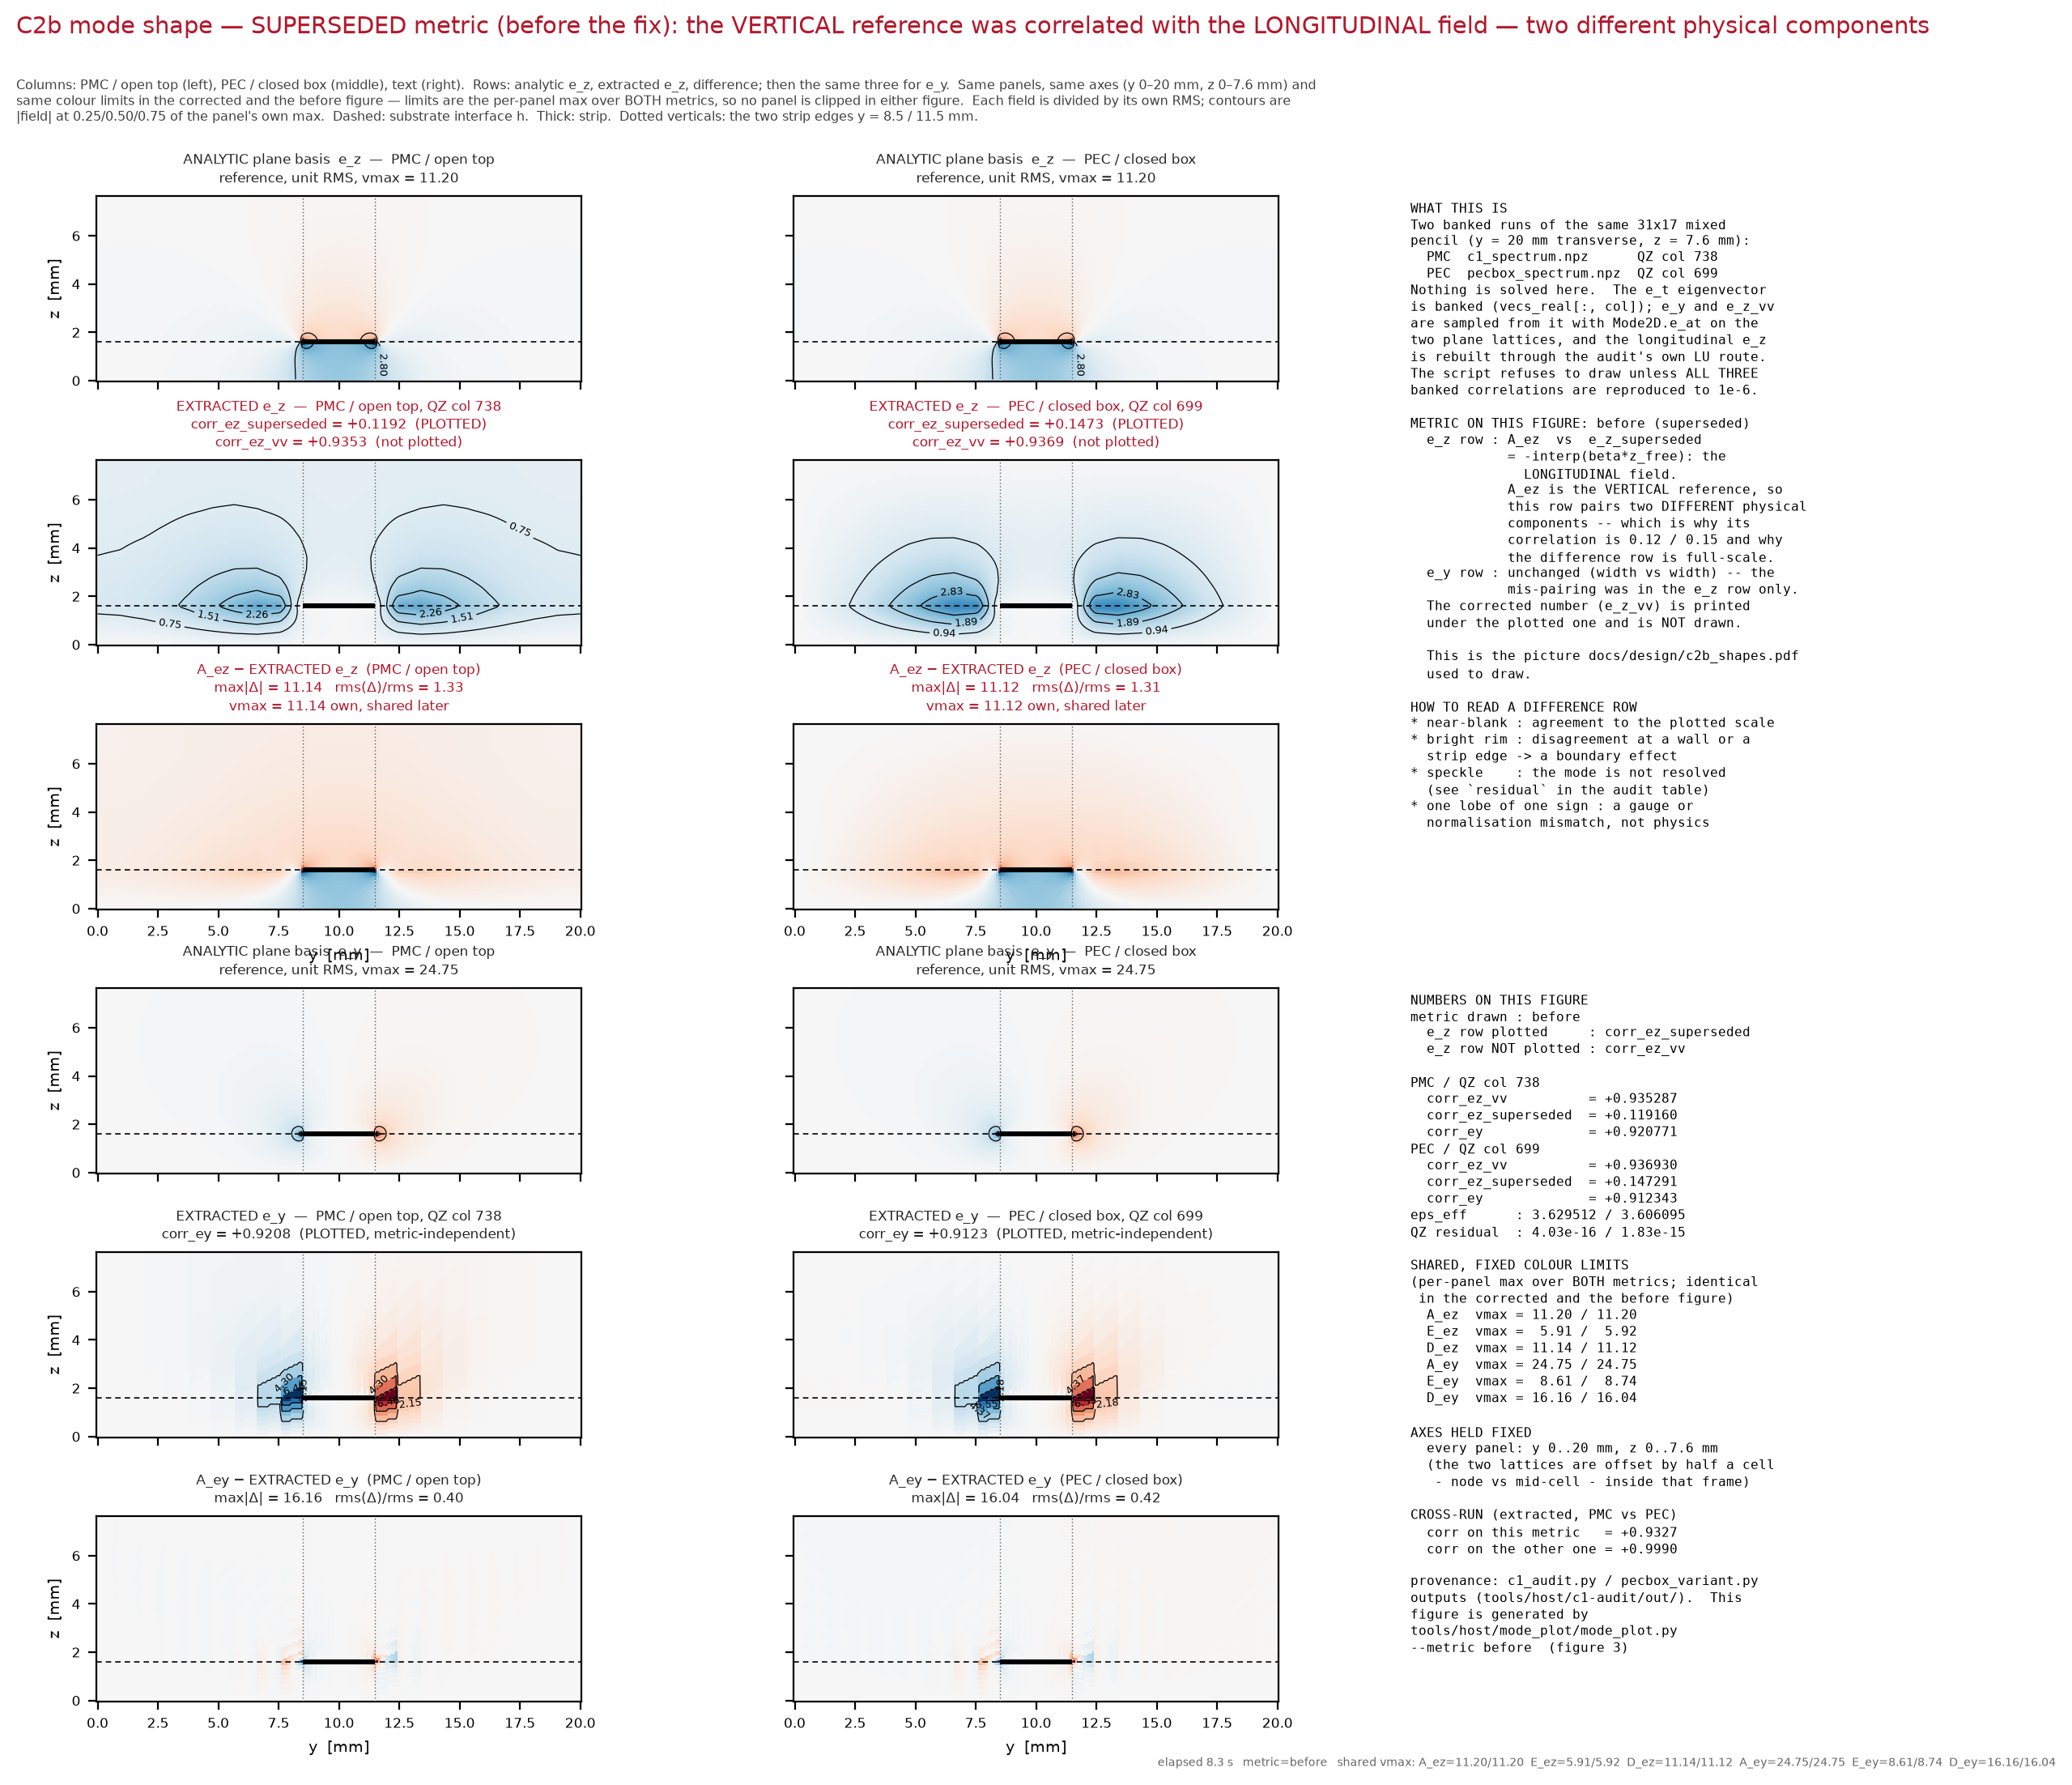
\includegraphics[width=0.95\textwidth]{../figures/mode_shape_mispaired_before.png}
  \caption[The superseded comparison: an analytic vertical reference correlated with an extracted longitudinal field.]{The
  superseded comparison. The $e_z$ row correlates two arrays that were never the same quantity: the analytic
  \emph{vertical} reference against the extracted \emph{longitudinal} field,
  $e_{z,\text{superseded}} = -\mathrm{interp}(\beta z_{\text{free}})$, on both banked runs (PMC QZ column $738$ of
  \texttt{c1\_spectrum.npz}, PEC QZ column $699$ of \texttt{pecbox\_spectrum.npz}, both $31\times17$). It reads
  $\mathrm{corr} = +0.1192$ (PMC) and $+0.1473$ (PEC), and the difference rows are correspondingly full-scale,
  $\max|\Delta| = 11.14$ and $11.12$ with $\mathrm{rms}(\Delta)/\mathrm{rms} = 1.33$ and $1.31$: the residual is
  larger than the field. The arithmetic is not wrong here, the \emph{pairing} is — a small correlation is the
  correct answer to a meaningless question, and that is why this row must not be read as the mode failing. \par
  The $e_y$ row is the built-in control: width against width, untouched by the mis-pairing, $\mathrm{corr} =
  +0.9208$ (PMC) and $+0.9123$ (PEC), drawn identically to the same row of
  Figure~\ref{fig:mode-shape-corrected}. The correct statistic for the $e_z$ row is printed beneath the plotted
  number on each extracted panel and is deliberately not drawn: $+0.9353$ and $+0.9369$.}
  \label{fig:mode-shape-mispaired}
\end{figure}

\begin{figure}[H]
  \centering
  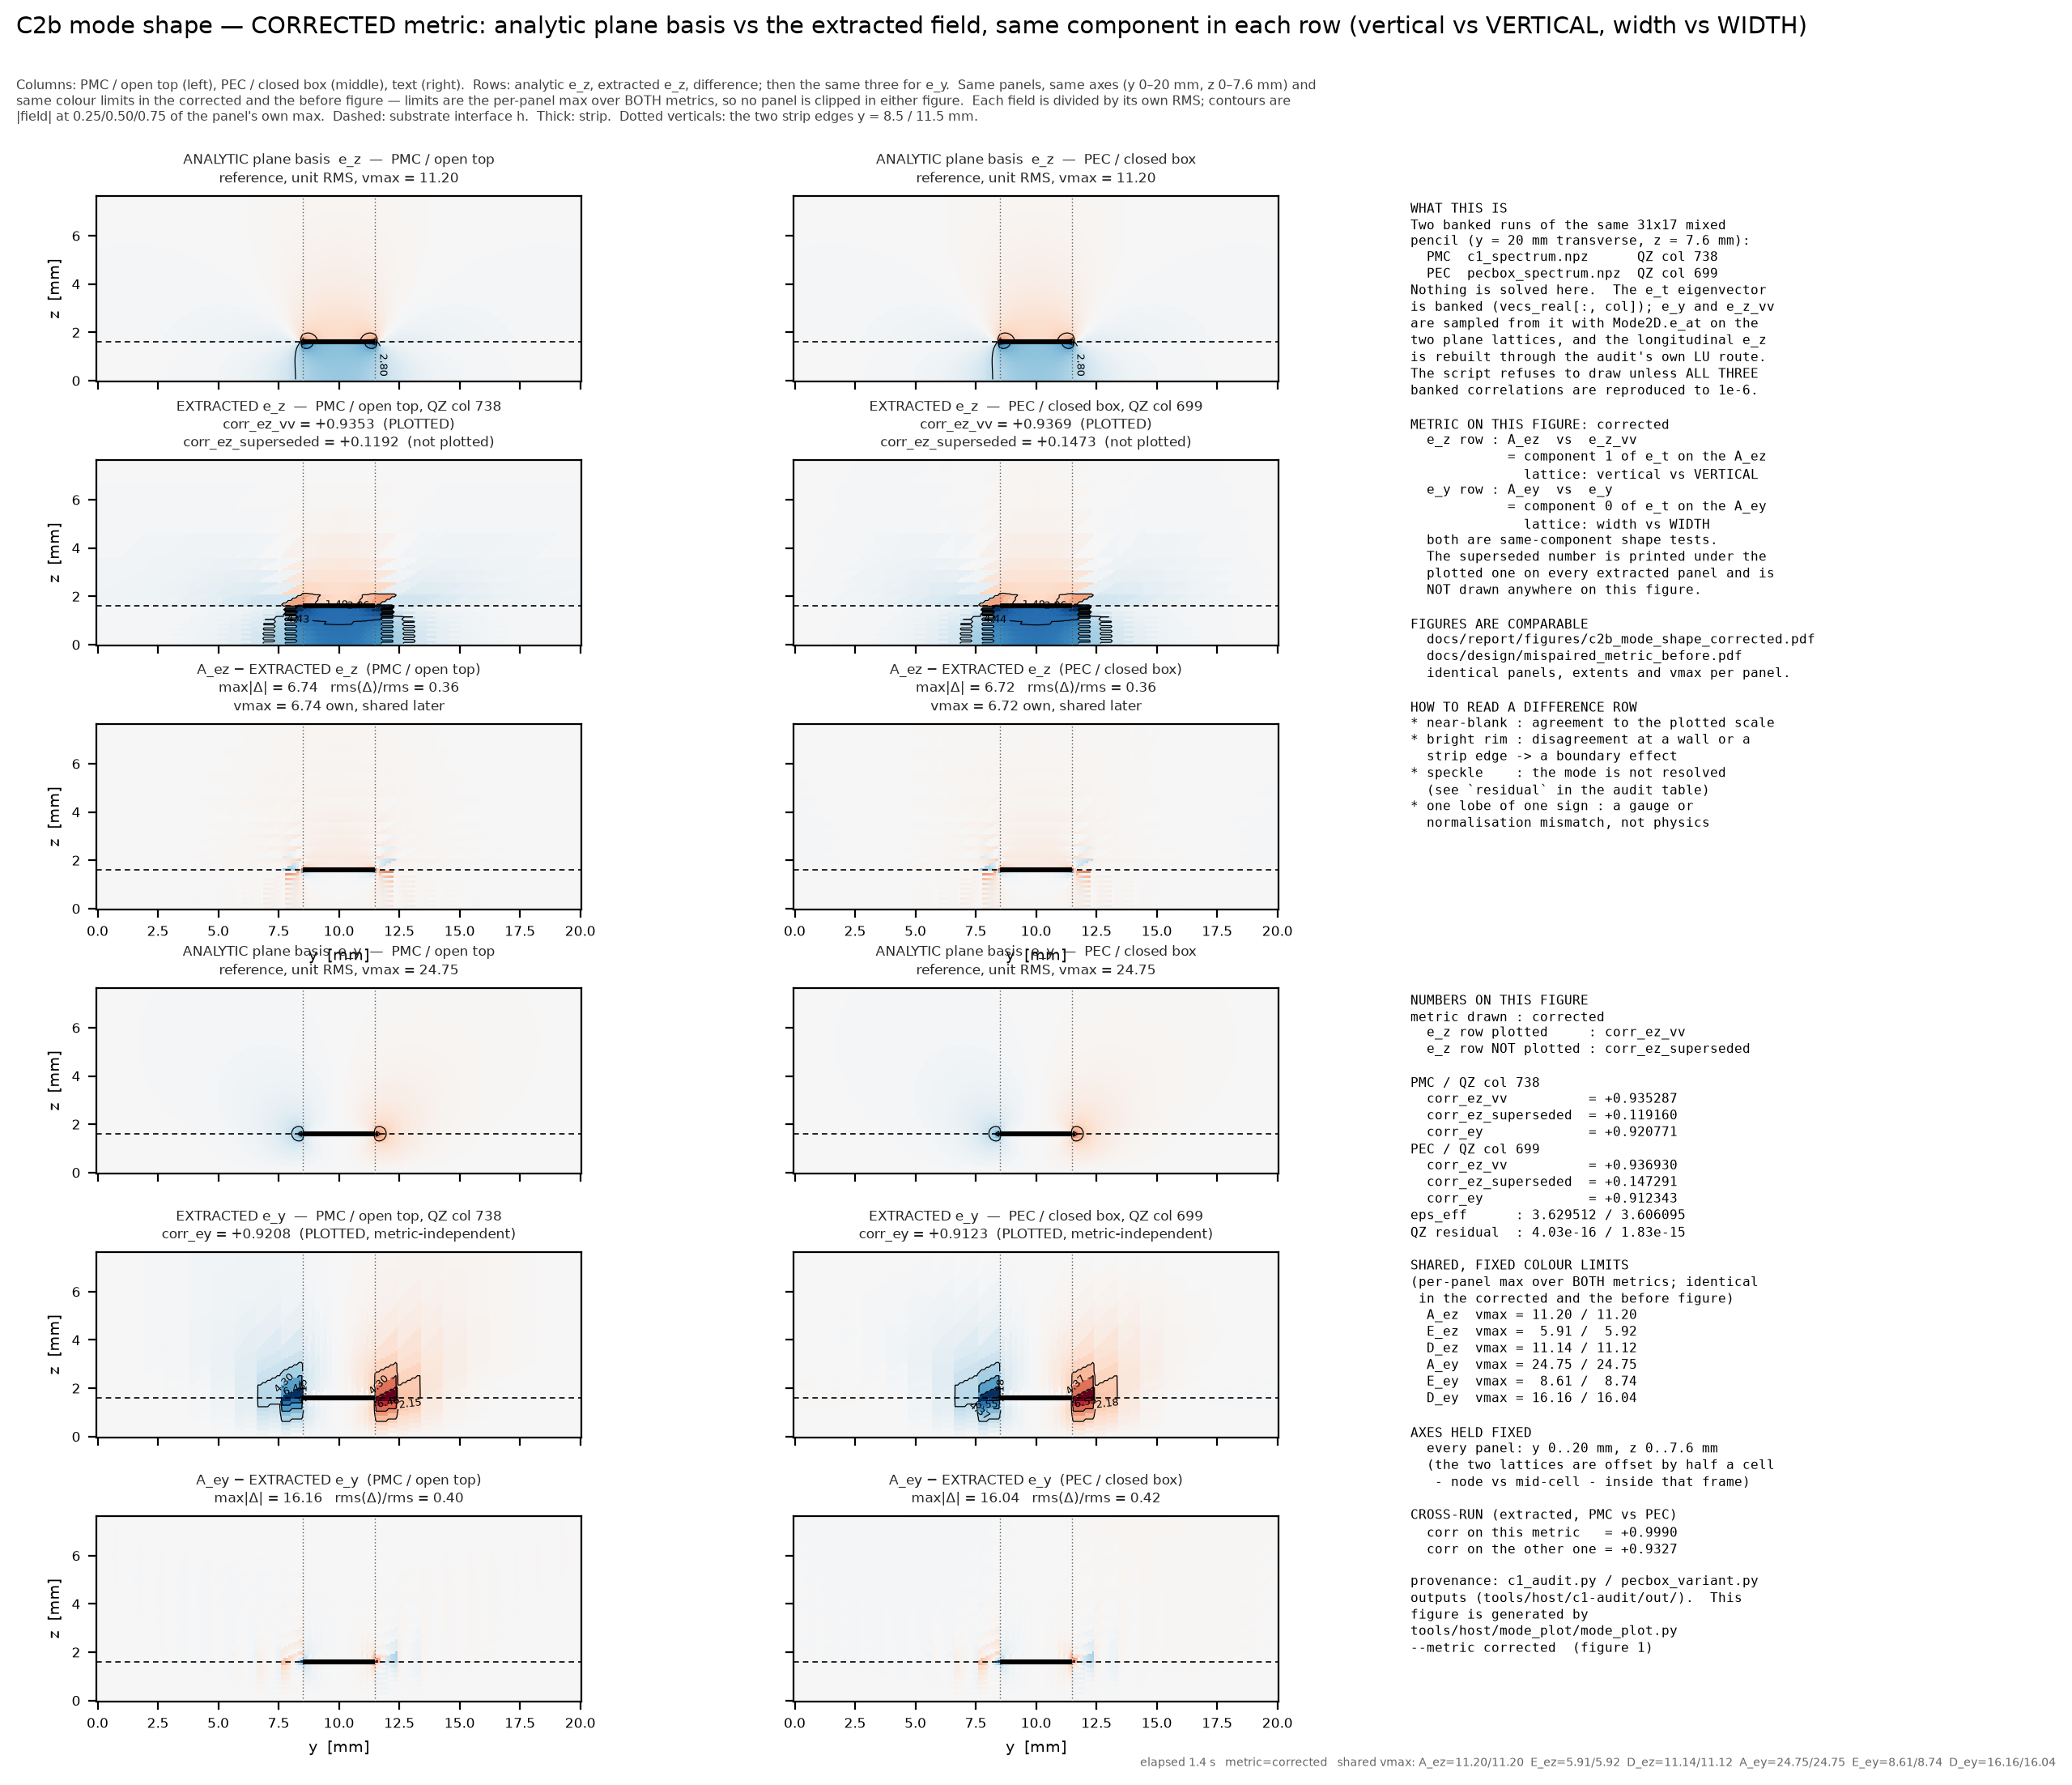
\includegraphics[width=0.95\textwidth]{../figures/mode_shape_corrected.png}
  \caption[The corrected comparison: the same components paired vertical with vertical.]{The corrected
  comparison: same banked runs, same panels, same extents, same per-panel colour limits, one row redrawn. The
  $e_z$ row now pairs like with like — component~$1$ of the banked $e_t$ eigenvector sampled on the
  $A_{ez}$ lattice against the analytic vertical reference, vertical versus vertical — and it reads
  $\mathrm{corr} = +0.9353$ (PMC) and $+0.9369$ (PEC). The difference rows fall to $\max|\Delta| = 6.74$ and
  $6.72$ with $\mathrm{rms}(\Delta)/\mathrm{rms} = 0.36$, and the two runs agree with each other on this metric at
  $+0.9990$ against $+0.9327$ on the superseded one. The reader's rule that this pair exists to teach: read which
  two things are being paired before believing which number. \par
  What the difference rows show is a near-blank field with a bright rim at the strip edges and at the substrate
  interface — disagreement concentrated where the discretisation is thinnest and where the reference field has its
  largest gradient, a boundary effect rather than a shape error. Because every extent and every per-panel limit is
  shared with Figure~\ref{fig:mode-shape-mispaired}, the two pages can be flipped between directly and any
  difference seen between them is the metric and nothing else.}
  \label{fig:mode-shape-corrected}
\end{figure}
      % \section{Mode shape: a cross-section field, and a comparison that was wrong}
\section{Results}
\label{sec:results}

\noindent\emph{Status: draft -- everything in this section is produced by a single script that runs in about six
seconds and whose numbers have been re-measured for this revision; the cavity frequency tables themselves are in
Section~\ref{sec:eigen} and are cross-referenced rather than repeated here.}

The report has so far been about structure: which operators, which identity, which bound. This section is about
what comes out. All three figures below are produced by one artefact, \texttt{examples/cavity\_resonance.py},
which builds the $10\times7\times5$ cavity of $1.0\times0.7\times0.5$ m, drives it for $300$ steps with a Ricker
pulse of nominal bandwidth \SI{400}{\mega\hertz} on a single $z$-directed edge near a corner, records the
following $1500$ steps of ring-down, and writes the spectrum, a field slice and the energy trace. The time step
is $\Delta t=1.907\times10^{-10}$ s from \eqref{eq:cfl}, so the recorded window is \SI{343}{\nano\second} of
simulated time, and the whole run takes about $5.5$ s on one core. There is no randomness anywhere in it, and the
figures regenerate byte-identically.

\subsection{The ring-down spectrum}
\label{sec:res-spectrum}

\begin{figure}[H]
  \centering
  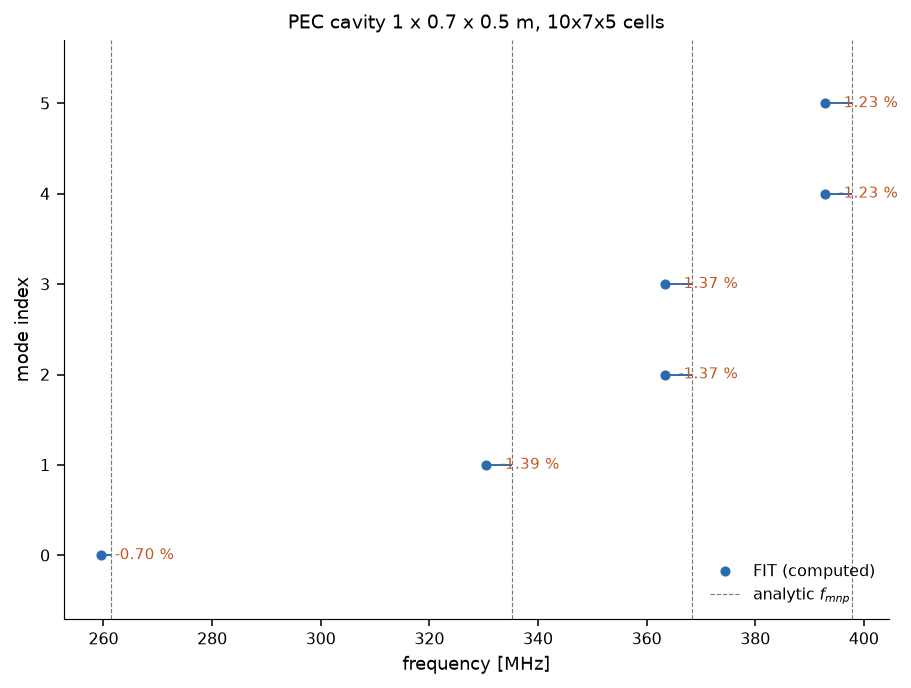
\includegraphics[width=0.78\textwidth]{../figures/cavity_spectrum.png}
  \caption{Resonances of the PEC box $1.0\times0.7\times0.5$ m on the $10\times7\times5$ grid, obtained by
  Fourier analysis of the $1500$-step ring-down that follows the drive. Computed frequencies are compared with
  the analytic modes of \eqref{eq:analytic}. The first six computed modes lie below their analytic counterparts,
  as a lumped material operator on a staggered grid must place them, and the two degenerate pairs are resolved as
  exactly equal pairs.}
  \label{fig:spectrum}
\end{figure}

Figure~\ref{fig:spectrum} is the frequency-domain output of a time-domain run: the field is stepped, the
ring-down is transformed, and the peaks of the transform are the resonances. That route to a spectrum is worth
having on its own, because it exercises the stepper rather than the eigensolver, and a mistake in the update
{\eqref{eq:leapfrog-h}--\eqref{eq:leapfrog-e}} would move the peaks. The six modes it finds are
$259.57$, $330.52$, $363.38$, $363.38$, $392.85$ and $392.85$ MHz against analytic values of $261.39$, $335.18$,
$368.42$, $368.42$, $397.74$ and $397.74$ MHz, a mean relative error of $1.213$\,\%, with the two degenerate
pairs reproduced to the last printed digit.

We deliberately do not tabulate those numbers again. The authoritative statement of the cavity spectrum is
Table~\ref{tab:cavity} and the order-of-convergence study is Table~\ref{tab:convergence}; both come from the
eigensolver of Section~\ref{sec:eigen}, which is the path that produces frequencies to a stated accuracy. What
Figure~\ref{fig:spectrum} adds is that the same spectrum is reachable from the time domain, that the extraction
is not doing anything delicate -- the peaks are far above the noise floor of a run whose energy is conserved to
rounding -- and that the two paths agree, which is a check on both.

The two pairs are degenerate because the box is not square in plan: the $363.38$ MHz and $392.85$ MHz modes each
come in a twofold set that the analytic count \eqref{eq:analytic} also produces, and their computed equality is
the symmetry of the discrete problem showing through. A solver that broke the pair apart by a fraction of a
percent would be telling us that its numbering or its stencil was not symmetric, so the printed pairs are a
sharper test than the mean error suggests.

\subsection{The field}
\label{sec:res-field}

\begin{figure}[H]
  \centering
  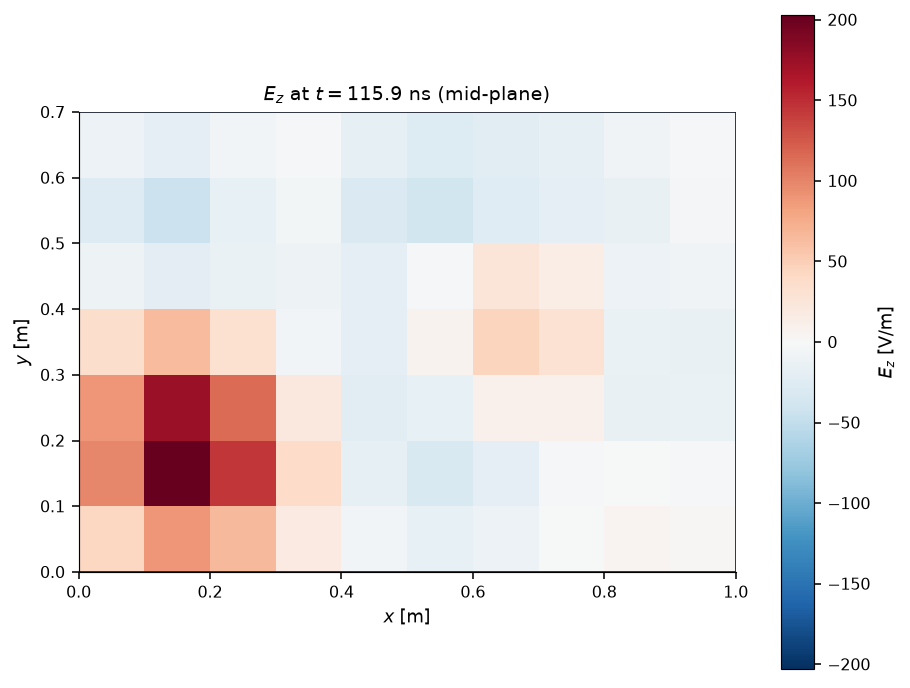
\includegraphics[width=0.72\textwidth]{../figures/cavity_field_z.png}
  \caption{The $z$ component of the electric field on the mid-plane of the cavity, taken at the moment the
  maximum field norm is reached during the drive. Sign changes across the box and the vanishing on the conducting
  walls are the features to look for: the pattern is the one the corresponding analytic mode predicts, with the
  nodal planes where they belong and the field tangential to the walls suppressed to zero.}
  \label{fig:field}
\end{figure}

Figure~\ref{fig:field} is the field map an engineer would ask for first, and it is the cheapest of the three to
read. It is a slice through the box at the instant of maximum field norm during the drive, so it shows the
excitation pattern rather than a single eigenvector -- the ring-down is a superposition, and a snapshot of a
superposition on a cut plane is honest about that. What the eye can check is qualitative but not soft: the sign
changes across the box are in the right places for the lowest modes of this box, and the field is zero on the six
walls to within the plotting resolution, which is the discrete counterpart of the boundary condition
\eqref{eq:leapfrog-pec}.

The slice is drawn by sampling the field on the nodes of the plane and interpolating from the edge-based unknowns,
which is the one piece of post-processing in the package that is not a plain reshape; it lives in
\texttt{viz.py} and it is the only place where a field component is moved from an edge to a point. Nothing in the
solver depends on it, and the figure is therefore evidence about the solution rather than evidence about the
pipeline that draws it.

\subsection{Energy in the same run}
\label{sec:res-energy}

\begin{figure}[H]
  \centering
  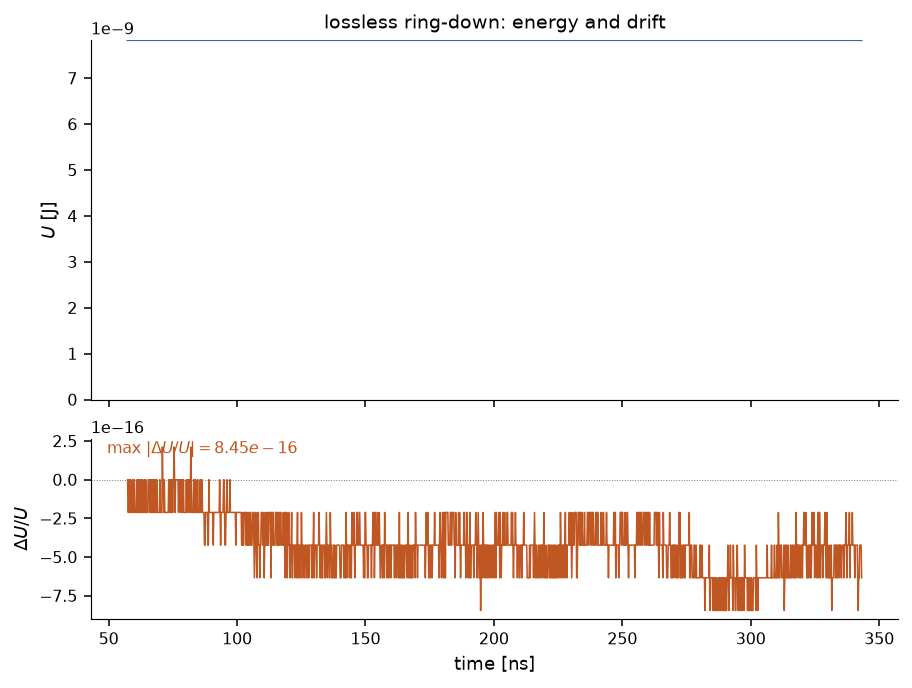
\includegraphics[width=0.85\textwidth]{../figures/energy_drift.png}
  \caption{Energy of the driven cavity run. Top: the invariant \eqref{eq:invariant} over the whole $1800$ steps,
  including the drive, on a linear scale on which the \SI{300}{} driven steps and the following
  \SI{343}{\nano\second} of ring-down are indistinguishable from a constant. Bottom: the relative drift on a
  logarithmic scale, which is where the interesting structure is -- the residual is at the level of a rounding
  floor, and it does not grow with step count.}
  \label{fig:energy}
\end{figure}

Figure~\ref{fig:energy} is the same run seen from the point of view of Section~\ref{sec:energy}. On a linear
scale the energy is a horizontal line: the drive injects power for $300$ steps, the source is switched off, and
the ring-down that follows neither gains nor loses energy at any scale a plot can show. The lower panel is the
same quantity on a logarithmic axis, and it is the informative one. The peak relative deviation over the recorded
portion is $8.451\times10^{-16}$, which is a few multiples of $\epsilon_{\mathrm{mach}}$ -- the rounding of a
double-precision sum of a few thousand positive terms, not a truncation error that a finer grid would reduce.

This is the strongest single statement in the report, and it is worth being precise about what it means. It is
not that the scheme conserves energy approximately, or that the drift is small enough not to matter. It is that
the quadratic form \eqref{eq:invariant}, evaluated on the staggered pair $(\mathbf{e}^{n},\mathbf{h}^{n-1/2})$
with its sign-indefinite cross term, is preserved to rounding by the update as implemented, on a run of $1800$
steps including a driven phase, in a cavity with conductor losses set to zero by construction. The comparison
against the three neighbouring candidate forms is in Table~\ref{tab:candidates} and is not repeated here; the
figure shows the winning candidate on a run long enough to make the point once, rather than the discrimination
that section already made.

\subsection{The time-domain checks}
\label{sec:res-time}

Two measurements in the suite are time-domain measurements, and both are quoted here because they are the only
quantitative checks on the stepper that do not involve a cavity.

The first is the conservation study of Table~\ref{tab:candidates}: a $12\times10\times8$ grid, random initial
fields, $500$ undriven steps, measured drift $1.298\times10^{-15}$ with the tolerance of the test set at $10^{-6}$
so that it asserts structure rather than a number. The same section records $8.45\times10^{-16}$ over $1500$ steps
and $1.669\times10^{-15}$ on a live run of the conservation test. We add only that these three values differ by a
factor of order two in the last digit and not in the exponent, which is the signature of a rounding floor sampled
at three points: there is no trend with step count to extrapolate, and no drift to blame on anything.

The second is the wave speed. On a $40\times6\times6$ grid with $h=0.02$ m, a broadband pulse whose nominal
wavelength spans about ten cells, and a probe ten cells downstream of the source, the front arrives at
$0.904\,c_0$ -- measured relative to the distance travelled and the elapsed time, with arrival defined as the
first sample above five per cent of the probe's peak. Section~\ref{sec:dispersion} derives the relation
\eqref{eq:phase} and shows that this number is what the formula predicts for a front whose leading edge sits at
about four cells per wavelength; the deficit is a second-order bias with the sign the theory gives it, it
vanishes as $h/\lambda\to0$, and it is neither an instability nor a symptom of a wrong operator. In the same
test, the field at the probe is exactly zero in the first three steps after the source is excited, which is the
causality check on a scheme that advances both fields at once.

\subsection{What this establishes, and what it does not}
\label{sec:res-scope}

It is worth separating the two, because the results above are strong and narrow at the same time.

What the results establish is the following. The discrete operators satisfy the identities of
Section~\ref{sec:theory} exactly, in integer arithmetic and independently of the mesh metric. The discrete
energy is conserved by the stepper to round-off over thousands of steps, which is a statement about the update
and not about the accuracy of its solution. The cavity spectrum converges at second order and lies within about
one per cent of the analytic box spectrum on the coarse grids used here, with the errors decreasing
at the rate Table~\ref{tab:convergence} measures. And a wavefront travels at a speed consistent with the
dispersion relation of the scheme, with the correct sign and the correct size.

What the results do not establish is anything about radiation. Every number in this section comes from a problem
whose boundary is a perfect conductor, so no field ever has to leave the domain, and the solver was never asked
to do the thing that an open-region problem demands: absorb an outgoing wave without reflecting it, and compute a
field at a distance. There is no absorbing boundary condition in the package, no near-to-far-field transform and
no port, and consequently there is no scattering result, no impedance and no $S$-parameter here. A cavity is the
easiest problem in computational electromagnetics precisely in this respect -- it is the one case where the
boundary condition costs nothing -- so the accuracy quoted above should be read as an accuracy about the
interior problem, on which every open-region result will later rest but none of which it can replace.

Closing that gap is the next milestone rather than a refinement of this one, and the acceptance test for it is
stated in terms of a quantity we cannot currently compute at all. Until a scatterer's bistatic radar cross
section has been compared with a Mie series, the honest summary of the present state is that the machinery is
verified and the physics it can address is still enclosed by walls.
    % \section{Results}
\section{An open problem: an 8\% passivity excess on a graded mesh}
\label{sec:openproblem}

\noindent\emph{Status: draft -- a problem statement. Nothing here is computed, no new field solve stands behind it,
and the one run that would settle it has been registered, priced and not made. Every number carries the line of
\texttt{decisions.md} that holds it.}

\subsection{The observation}
\label{sec:openproblem-observation}

At \SI{7.833566}{\giga\hertz} the port-plane reflection is $|S_{11}| = 0.013677$ and the transmission is
$|S_{21}| = 1.039055$, both from the single record \texttt{board\_cw\_7.8333GHz.npz}
(\texttt{decisions.md:3096}), so $|S_{11}|^2 + |S_{21}|^2 = 1.079823$: reflected and transmitted power together
exceed the incident power by $7.98$ per cent (\texttt{decisions.md:1394}). No gain term can deliver it: the only
damping is the perfectly matched layer (\texttt{decisions.md:83-88}).

The same excess appears in coordinate space, and that is the form we argue in. Over nine station planes from
\SI{10.4}{mm} to \SI{20.0}{mm} -- \SI{9.6}{mm} of a \SI{23.5}{mm} line -- the circuit quantity
$\tfrac12\operatorname{Re}(v\,i^{*})$ rises $8.4742$ per cent in power end to end, $4.1509$ per cent in amplitude
(\texttt{decisions.md:3102}), while the same nine cross-sections reduced as a time-averaged Poynting flux fall
$3.0723$ per cent (\texttt{decisions.md:1472}).

The profile is not monotone: it peaks at station 8, station 9 sits $0.13$ per cent below the peak in the full-step
and the half-step record alike, and nothing jumps at the strip interface (\texttt{decisions.md:1424}). It saturates
and turns over, which neither an instability nor a sink would do. Nor is it the whole line: the last station stops
\SI{12.2}{mm} short of the far wall, so the excess belongs to \SI{9.6}{mm} of it (\texttt{decisions.md:3323}).
Halving the step, mesh unchanged, over $16\,067$ steps moves the growth from $1.039055$ to $1.039043$, the excess
from $8.4742$ to $8.4549$ per cent and $\alpha$ by $-0.030$ per cent for \SI{5547.6}{s}
(\texttt{decisions.md:1408}, \texttt{decisions.md:1430}, \texttt{decisions.md:1434}); \texttt{dt\_scale} refines
time only (\texttt{decisions.md:1428}).

\subsection{What it is not}
\label{sec:openproblem-not}

\emph{Not the field update.} No parameter of the update can add power, and the part a test can hold is held:
\texttt{pec\_conservation} pins the relative drift of the mixed-state invariant below $10^{-10}$ over a thousand
steps on a box with PEC walls (\texttt{tests/test\_energy.py:157}, \texttt{decisions.md:87}). The excess is
$7.98\times10^{-2}$, eight orders above that drift, and halving $\dd t$ moves it by $0.030$ per cent of itself.

\emph{Not the reference division.} The division that would inflate $|S_{21}|$ is at
\texttt{emfit/studies.py:1984-1990}, inside \texttt{if reference is not None:}, with the power column at
\texttt{:2005-2008} under the same guard, and \texttt{reference\_used} (\texttt{emfit/studies.py:2153}) is
\texttt{False} on all six board captures (\texttt{decisions.md:2987}): the named mechanism has no referent in the
stored data. The two amplitude routes left, power and projection, agree to $2.36\times10^{-3}$ and both exceed
unity (\texttt{decisions.md:3100}).

\emph{Not the 5.9 per cent effective permittivity.} The one material-side number of that size is the $5.9$ per cent
between measured $\eps_{\mathrm{eff}}$ and the static Hammerstad-Jensen value, and it is not an error: at
\SI{5.827786408}{\giga\hertz} the measurement is $3.541823$ against $3.343938310$ static, every dispersion closure
in the tree lies between those, and a quasi-static open-boundary formula is not a like-for-like reference
(\texttt{decisions.md:3010}, \texttt{decisions.md:3016}). The static value is retired in both directions, neither
solver-error evidence nor validation (\texttt{decisions.md:2899}, \texttt{decisions.md:2901}), and the family
explains sign and order only, its spread being the size of the effect (\texttt{decisions.md:3086}).

\emph{Not the coupon floor.} The instrument has one calibration, a matched uniform coupon at \SI{5.8278}{\giga\hertz}
with $|\gamma| = 0.0328$, on which the flux must be flat and is not: \texttt{sx\_station} decays $6.2646$ per cent
over \SI{6.4}{mm} where the circuit quantity decays $1.9205$ per cent, the halves agreeing to $1.1\times10^{-3}$
(\texttt{decisions.md:1446}). That tilt is mesh-independent, rate ratio $1.0044$, so not truncation
(\texttt{decisions.md:1448}). Its settledness, $1.1\times10^{-3}$, sits a factor $79.8$ below the board excess of
$7.98\times10^{-2}$; that factor is arithmetic between two stored figures and nothing else, the record forbidding
the floor to be combined with, subtracted from or used to bound $1.079823$, the two not being on the same footing
(\texttt{decisions.md:3084}). What separates them is sign: the coupon artefact is a decay of about one per cent per
millimetre, a spurious decay cannot manufacture a growth at any mesh, and scaling the board figure by it was
computed and rejected (\texttt{decisions.md:1460}).

One mechanism survives all four, the per-station power reading on a graded mesh (\texttt{decisions.md:3090}).

\subsection{The four rivals, and what would separate them}
\label{sec:openproblem-rivals}

The scored quantity is $R$, last-station power over first: $R = 1.084742$ at the anchor's cell
(\texttt{decisions.md:3341}). Each rival predicts $R$ at the \SI{0.05}{mm} cell the test would build, from the
anchor value scaled to that cell and widened by the only scatter on file, $1.0849$ against $1.0968$, about $1.1$
per cent (\texttt{decisions.md:3335}); no reading of $R$ resolves less than that.

\begin{table}[H]
  \centering
  \caption{The four rivals and the number each predicts at the cell the test of Section~\ref{sec:openproblem-c5}
  would build (\SI{0.05}{mm}, \texttt{n\_sub} 32; \texttt{decisions.md:3297}, \texttt{decisions.md:3341}). Bands
  from \texttt{decisions.md:3345-3347}, widened by the $1.1$ per cent floor of \texttt{decisions.md:3335}; the
  port-near row from \texttt{decisions.md:3331}, \texttt{decisions.md:3333}, \texttt{decisions.md:4324}.}
  \label{tab:openproblem-rivals}
  \begin{tabular}{@{}lp{3.6cm}cc p{4.5cm}@{}}
    \toprule
    Rival & Claim & $R$ at \SI{0.05}{mm} & Band & Separated from the others by \\
    \midrule
    H & the rise is scale-free, not a property of the mesh & $1.0847$ & $[1.0728,\,1.0967]$
      & the cell refinement alone; disjoint from both others \\
    \addlinespace
    R$'$ & the rise is second order in the cell & $1.0212$ & $[1.0101,\,1.0324]$
      & the cell refinement alone; overlaps L \\
    \addlinespace
    L & first order in the cell, named although nothing on file predicts it & $1.0424$
      & $[1.0310,\,1.0538]$ & as R$'$; a reading here falsifies both others \\
    \addlinespace
    port-near & near-field contamination at the port, decaying over \SI{2.77}{mm} & $1.084742$
      & $[1.0728,\,1.0967]$ & not the cell refinement at all: the four port planes \\
    \bottomrule
  \end{tabular}
\end{table}

A reading in the H band falsifies R$'$ and L, one in either of the others falsifies H, and one below $1.0101$ or
above $1.0967$ falsifies every named rival and is recorded as a class (d) outcome rather than resolved by preference
(\texttt{decisions.md:3351-3356}). R$'$ and L overlap, so a reading between $1.0310$ and $1.0324$ chooses neither --
which is why the first-order rival was named at all, so that the gap between the other two is never read as an empty
band (\texttt{decisions.md:3347}, \texttt{decisions.md:3357}).

\subsection{The test we registered, and what we admitted about it}
\label{sec:openproblem-c5}

The lever is \texttt{n\_sub} $16 \to 32$: the cell halves to \SI{0.05}{mm}, the mesh becomes $644\times400\times92$
-- $4.842$ times the anchor's cells -- and the steady resident set goes from $2.68$\,GiB to $12.98$\,GiB
(\texttt{decisions.md:3297}, \texttt{decisions.md:3307}). The step count doubles with the cell's halving, $8034$ to
$16\,068$ (\texttt{decisions.md:4485-4492}), so the wall time is $2936.7 \times 4.842 \times 2.0 = 28\,439.6$\,s,
$7.90$\,h, plus the gate, itself conditional on the anchor being re-run in a quiet window
(\texttt{decisions.md:4497-4499}). One memory distinction, and we keep it: $12.98$\,GiB is the steady figure for
the run as registered, and the only peak on file, $13.06$ to $13.09$\,GiB, derived and not measured, is the
post-lever peak, $10.09$\,GiB steady, leaving $2.22$ to $2.25$\,GiB against the $15.30659$\,GiB host limit
(\texttt{decisions.md:3311}, \texttt{decisions.md:4494-4496}). At nine point seven times the anchor, the verdict on
file is that the run is inadmissible as it stands (\texttt{decisions.md:3361}).

The amendment we then wrote is the part of this chapter we would most like attacked. What was claimed first stands
as registered; what changed is what the test is said to decide (\texttt{decisions.md:4480-4483}). It decides H
against R$'$ and against L, whose bands do not overlap; it does not decide R$'$ against L, whose bands do; and it
does not close the port rival, which the four displaced port planes exist to test
(\texttt{decisions.md:4473-4478}). The bands were not redrawn, because a pre-registration edited after a result
exists has failed at its only job (\texttt{decisions.md:3090}). One run scores two questions: passivity is read
from the same capture, $1.0212$ under R$'$ against $1.0849$ under H (\texttt{decisions.md:3359}). Only this lever
moves the cell.

\subsection{What we would check first}
\label{sec:openproblem-six}

\begin{enumerate}[leftmargin=1.6em,itemsep=3pt]
  \item \textbf{Measure the absorber before trusting the wall.} The board runs twelve cells of it at \SI{0.1}{mm}
        (\texttt{decisions.md:4403}), under the twenty-cell default of a layer whose measured table calls twenty
        cells modest and forty what a real absorber wants (\texttt{emfit/pml.py:32-36}). What is its reflection?
  \item \textbf{Price the fan-outs the mesh leaves out.} The strip is one uniform width, $30$ cells
        (\texttt{decisions.md:1369}), while the copper fans \SI{2.0}{mm} to \SI{3.0}{mm} before the port plane and
        \SI{3.0}{mm} to \SI{0.64}{mm} past the far one (\texttt{decisions.md:3162}): what do the steps cost?
  \item \textbf{Name the wave before comparing ratios.} \texttt{z0} enters only where a caller wants an absolute
        power wave, never in a ratio (\texttt{emfit/ports.py:31}), yet $|S_{11}|^2+|S_{21}|^2$ sums a station fit
        with a normalised amplitude whose power twin sits beside it (\texttt{emfit/studies.py:1990}, \texttt{:2004}).
  \item \textbf{Show the record is long enough where it is shortest.} The upper band runs $8034$ steps at
        \SI{7.833566}{\giga\hertz} so its tone lands on a DFT bin, where the pulse's $9600$ would sit at
        \SI{8.0131}{\giga\hertz}; the band below is clean, passivity $1.00046$ at \SI{3.667}{\giga\hertz}
        (\texttt{decisions.md:1369}, \texttt{decisions.md:1378}).
  \item \textbf{Check the strip's cell where it is used, not only where it is assigned.} The static audit clears
        the material map and its dual interface average (\texttt{decisions.md:2339}), then names what it cannot
        reach: the staircased strip, the port excitation, the strip and interface assignment
        (\texttt{decisions.md:2343}). The extractor reads a gap voltage there (\texttt{emfit/studies.py:2766-2767}).
  \item \textbf{Move the port, not the mesh.} Four port planes at $\pm 2$ and $\pm 4$\,mm are written down and
        none has been run (\texttt{decisions.md:4418}); the near field decays over \SI{2.8}{mm}, so \SI{4}{mm} moves
        it by its own size (\texttt{decisions.md:4435}); the repeat ran and returned exactly zero, so scoring
        them needs a resolution bought from the estimator window instead
        (\texttt{decisions.md:4361-4393}).
\end{enumerate}

\subsection{The request}
\label{sec:openproblem-request}

Here is the check we have not done: we have never refined the cell at \SI{7.8333}{\giga\hertz} on a record that can
be read on the admitted branch, and until we do, an eight per cent excess in the power budget of a lossless line is
a statement about our own extraction before it is a statement about the discretisation. Time we have refined and
the growth survived it. Space we have not, and we know why: nine point seven anchor runs, thirteen gigabytes of
resident memory, and a price arithmetically wrong by four in the script everyone would quote.

Two replies would be worth more than agreement: a fifth mechanism we have not named, with the observation that
would distinguish it from the mesh-and-estimator rivals; or a demonstration that one of the four is not decidable by
the levers we hold, which would be the cheaper result. What would not help is a reading of $1.079823$ as plausible:
it is $8.4742$ per cent in power, \SI{0.353}{dB}, on a line whose material model contains no loss and whose only
damping is a layer outside the box.
 % \section{An open problem: an 8\% passivity excess on a graded mesh}
\section{Outlook}
\label{sec:outlook}

\noindent\emph{Status: draft -- the milestone list and the acceptance criteria are transcribed from the roadmap
that governs the work; the open problems are stated as problems, and none of the milestones after M0 is claimed
to be working.}

What remains is not a refinement of what is finished. The cavity solver of Sections~\ref{sec:eigen}
and~\ref{sec:results} is accurate and its energy is exact, but the package cannot yet radiate: there is no
absorbing boundary, no near-to-far-field transform and no port, so every problem it can address is enclosed by
walls. The roadmap is therefore a list of capabilities rather than a list of improvements, and each entry carries
an acceptance test expressed in terms of a quantity the code cannot currently compute. That is deliberate: a
milestone is done when its number is reproduced by the test suite, not when the module exists.

\begin{table}[H]
  \centering
  \caption{The roadmap. Status, deliverable and acceptance criterion for each milestone, in dependency order
  rather than order of value. Only M0 is complete; M1 and M5 are in progress.}
  \label{tab:milestones}
  \begin{tabular}{@{}lp{1.8cm}p{5.6cm}p{5.6cm}@{}}
    \toprule
    & Status & Deliverable & Acceptance criterion \\
    \midrule
    M0 & done & time-domain core with the exact invariant; dense cavity eigensolver & thirty tests pass; box
    modes within $1.3$\,\% ($1.213$\,\% coarse, $0.615$\,\% fine) and second-order ratio $0.507$ \\
    M1 & in progress & first-order Mur absorbing condition on the six outer walls, then a stretched-coordinate
    PML layer & PEC sphere of radius $0.1$ m: bistatic RCS within $0.5$ dB of the Mie series at $ka=1$
    (\SI{477}{\mega\hertz}) and $ka=3$ \\
    M2 & planned & near-to-far-field transformation over a Huygens surface, one transient run transformed &
    half-wave dipole at \SI{300}{\mega\hertz}: $\operatorname{Re}Z_{\mathrm{in}}=73\pm5$\,\si{\ohm},
    $|\operatorname{Im}Z_{\mathrm{in}}|<20$\,\si{\ohm}, $2.15\pm0.15$\,dBi \\
    M3 & planned & two-dimensional modal port eigenproblem, mode overlaps, de-embedding & WR-90 waveguide,
    TE$_{10}$ at \SI{6.557}{\giga\hertz}: $|S_{11}|<-30$\,dB, $|S_{21}|=1.000\pm0.001$, phase within
    \SI{1}{\degree} \\
    M4 & planned & KiCad s-expression reader, staircase voxelisation, stack-up to material parameters & microstrip
    $Z_0$ within $5$\,\% of Hammerstad--Jensen; patch resonance within $3$\,\% of $c/(2L\sqrt{\eps_{\mathrm{eff}}})$ \\
    M5 & in progress & gradient null-space deflation followed by a matrix-free eigensolver beyond the dense
    threshold & $10^5$ free edges, six modes in under five minutes, within $0.1$\,\% of a dense solve \\
    M6 & planned & $\mathbf{A}$--$V$ magnetoquasistatics with eddy currents; parareal time integration & aluminium
    slab, skin depth $2.7$ mm at \SI{1}{\kilo\hertz} and $11.0$ mm at \SI{60}{\hertz}, within $2$\,\% \\
    \bottomrule
  \end{tabular}
\end{table}

Two of these entries are gates rather than features. M1 is the gate to every open-region question: without an
absorbing boundary there is nothing to compare with a Mie series, and without a far-field transform there is no
radiation pattern to draw, so M2 has no meaning until M1 has produced a field that leaves the domain. M5 is the
gate to every engineering-sized geometry: the dense solver of Section~\ref{sec:eigen} refuses more than $3000$
free edges, which is a cavity of a few wavelengths and no more, and nothing about a printed antenna fits inside
that budget. The other four are independent of each other, which is why they can be reordered as time and
interest allow.

\subsection{Open problems}

The following are difficulties we do not yet know how to price, not features we have promised. Each is stated as
the question we would have to answer before the corresponding milestone could be called finished.

\begin{enumerate}[leftmargin=1.6em,itemsep=3pt]
  \item \textbf{Whether the dispersion is worth repairing.} At about four cells per wavelength the tracked front
        travels at $0.904\,c_0$, and \eqref{eq:phase} says why. The open question is what to do about it: raise
        the order of the spatial operator, refine until the bias is negligible, or accept it and quote
        frequencies with a known sign of error. Higher order means giving up the two-point stencil on which the
        exact identity \eqref{eq:invariant} rests, so the cheap repair and the strong conservation result are in
        direct competition, and we do not know which we would choose.
  \item \textbf{The staircase error on curved geometry.} Voxelisation of a curved surface produces a boundary
        off by up to half a cell, and the resulting frequency error is not second order. A patch antenna imported
        from a layout file will be a staircase, and by how much that degrades the resonance is unknown to us; it
        may be that a fine local grid is enough, or it may be that a conformal treatment of the boundary is
        unavoidable and the structured-grid advantage is lost exactly where it is most wanted.
  \item \textbf{Deflating the null space at scale.} The gradient modes that make \eqref{eq:geneig} singular
        number in the thousands on the grids that matter, and the projector that removes them is a dense-ish
        operator applied inside an iterative solve. Whether the deflated iteration converges in a time an engineer
        will wait for, and whether it holds the $0.1$\,\% accuracy the dense path gives, is the substance of M5;
        the shift-invert route was tried and rejected, which tells us the obvious approach is wrong but not that
        the replacement is right.
  \item \textbf{The global time step.} The bound \eqref{eq:cfl} is set by the smallest cell anywhere, so one
        narrow gap or one thin conductor dictates the step count for the whole domain, and a graded grid can
        multiply the number of steps by four orders of magnitude. Local time stepping is the textbook answer and
        it interacts badly with an exact global invariant, since a scheme with different steps in different
        regions does not have a single conserved quadratic form of the simple sort.
  \item \textbf{Where the boundary goes.} Mur's condition and a Berenger layer both assume an outgoing wave and
        both are approximate on a staggered grid, and the reflection they leave behind sets the floor on any
        scattering result. Absorbing more than $20$ dB, and then more than $40$ dB, is a numerical question we
        have not answered; and a PML needs a diagonal tensor material in the layer, which the present scalar
        material layer cannot express, so M1 begins with an extension of the data structure rather than with an
        algorithm.
\end{enumerate}

\subsection{Scope}

We want to be plain about what the report as a whole claims. \texttt{emfit} is, today, a verified solver for
closed, isotropic, lossless problems on structured grids: it conserves the discrete energy to rounding, it
reproduces the analytic spectrum of a conducting box to about one per cent on coarse grids with second-order
convergence, and it propagates a wavefront at the speed its own dispersion relation predicts. It is not yet a tool
for the questions posed in Section~\ref{sec:theory} about antennas, laminate or scatterers, because those need a
field that leaves the domain and a port through which power is measured, and neither exists. The milestones above
are acceptance tests for that transition; the open problems are the parts of it we cannot yet cost. Progress will
be recorded here as it happens, including the parts that go badly.
    % \section{Outlook}
\section{Glossary}
\label{sec:glossary}

\noindent\emph{Status: a reading aid, not a source. Each entry fixes one sense of a term and points at the section
where that sense is defined and, where there is one, at the section where the quantity is measured. Where an entry
and a section disagree, the section governs: this list is not a place to record a new result.}

Several words here carry a narrower technical sense than their everyday one, ``exact'' being the obvious case, and
a few numbers acquired names that drifted away from the quantities they were computed from. The entries below fix
the senses in the order the terms are met, from Section~\ref{sec:theory} to Section~\ref{sec:worked}, and each
carries the distinction that the corresponding section had to keep straight. An entry that ends with a trap is a
mistake that was made in this report and then corrected, listed so that it is not made twice.

\begin{description}[leftmargin=1.6em,style=nextline,itemsep=4pt]

  \item[Finite integration technique (FIT).]
        A discretisation of Maxwell's equations on a pair of interlocked cell complexes, primal and dual, in which
        the curl and divergence operators are integer incidence matrices and the metric enters only through the
        diagonal Hodge star matrices. What is exact in it is the topology (Proposition~\ref{prop:identities}); what
        is approximated is the constitutive relation and the time step. It is not an exact method, and this report
        does not call it one.

  \item[Primal and dual complex; degrees of freedom.]
        The primal complex is the hexahedral mesh of edges and faces; the dual complex is built on the dual cells
        whose vertices are the primal cell centres. The unknowns are line integrals of $\vec e$ along primal edges
        and of $\vec h$ along dual edges, so that a primal edge carries a voltage and a dual edge a magnetic
        voltage, and one degree of freedom belongs to each. Written bold lower case, with a tilde on a dual
        quantity; the notation table is Table~\ref{tab:notation}.

  \item[Topological operators and the exact identities.]
        The curl matrices $\Cmat$ (primal edges to primal faces) and $\Smat$ (dual edges to dual faces) and the
        gradient $\Gmat$ are sparse, integer, and satisfy $\Smat\Cmat=0$ identically. The discrete identities of
        Proposition~\ref{prop:identities} and \eqref{eq:identities} are consequences of the incidence matrices
        alone: they hold for any material, on any grid, at any time step. This is the part of the scheme that
        cannot be wrong, and it is the reason statements about topology and statements about accuracy are kept
        apart throughout.

  \item[Hodge star matrices.]
        $\Em$, $\Mm$ and $\Ms$: diagonal, positive, with entries assembled from cell measures and material
        constants, as in \eqref{eq:stars} and Section~\ref{sec:hodge}. They are the only spatial approximation in
        the scheme -- diagonal, measure-based, low order -- and every accuracy statement in this report is
        ultimately a statement about them.

  \item[Leapfrog update and the mixed-state invariant.]
        The electric and magnetic unknowns are staggered by half a step (\eqref{eq:leapfrog-h},
        \eqref{eq:leapfrog-e}), which is what makes the step explicit. The quadratic form \eqref{eq:invariant} is
        conserved to rounding (Sections~\ref{sec:invariant} and~\ref{sec:evidence}). Trap: the conserved form is a
        mixed-state quantity, in which the two fields are read half a step apart; it is not the instantaneous
        physical energy, which oscillates at twice the drive frequency even though the invariant does not move.

  \item[CFL bound.]
        The largest time step for which the explicit recursion is stable, \eqref{eq:cfl}, tabulated in
        Table~\ref{tab:cfl} against measured runs. It is set by the smallest cell anywhere in the domain, not by the
        average one. Trap: the bound is a statement about stability and not about accuracy, so stepping well below
        it does not remove the dispersion of Section~\ref{sec:dispersion}.

  \item[Numerical dispersion; grid-dependent phase velocity.]
        The dispersion relation \eqref{eq:dispersion} is exact for the scheme and gives the phase velocity through
        \eqref{eq:phase}, which falls below $c_0$ for every non-zero wave vector (Section~\ref{sec:dispersion}).
        The phase velocity is a property of the grid and the wavelength together, not of the medium, and on this
        grid it is measured per run -- $0.904\,c_0$ for the tracked front of the demonstration -- rather than
        assumed from the permittivity.

  \item[PEC and PMC as constraints on the unknown space.]
        A perfect electric or magnetic conductor is imposed by constraining the tangential unknowns on the
        boundary face, \eqref{eq:pec}; it is not a material and involves no approximation of its own. The cost is
        paid in degrees of freedom, which is why the boundary conditions of this report are described as
        constraints and can be argued about exactly.

  \item[Mur first-order absorbing condition.]
        A one-way condition, first order in the cell size, applied to the six outer planes; implemented in
        \texttt{abc.py} and measured in Section~\ref{sec:res-abc}, \eqref{eq:mur}, at about $-50$\,dB of
        reflection at normal incidence in two dimensions. It is one member of a family of local boundary
        conditions and is not ``the'' absorbing boundary of the report.

  \item[PML; matched lossy layer.]
        A graded artificial conductivity added in a shell around the domain, chosen so that the interface
        reflects little and the wave decays inside the shell; implemented in \texttt{pml.py}, measured in
        Section~\ref{sec:res-pml}, where it absorbs more deeply than the one-way condition does on the same
        geometry. Trap: neither mechanism is \emph{the} boundary of the report. Both are additions to the same
        array, both were measured at normal incidence only, and the sections that measure them
        (Sections~\ref{sec:res-abc} and~\ref{sec:res-pml}) are cited side by side rather than ranked.

  \item[Cavity eigenproblem and the gradient null space.]
        The resonance problem is the generalised eigenproblem \eqref{eq:geneig} on the interior edges, and it is
        singular: every gradient of a scalar potential is a null vector of the curl-curl operator at zero
        frequency. Those modes are physical only as the static limit and are removed by projection before the
        solve (Section~\ref{sec:eigen}). Trap: a small eigenvalue returned with no check against the null space is
        more likely to be a gradient mode than a resonance.

  \item[Port; wave port.]
        A port is the surface through which a known field enters and leaves the domain and on which the
        travelling-wave amplitudes are measured (Section~\ref{sec:sp-definition}). A wave port is one that
        carries the transverse mode profile of the line rather than a lumped terminal pair, which is what allows
        $a$ and $b$ to be defined on it and a power to be assigned to each.

  \item[Mode normalisation.]
        The transverse mode profile $\mathbf{e}_{\text{mode}}$ is scaled so that the mode carries $1$\,W, which
        for the line measured here fixes a voltage scale without the report printing a value for it. The port
        voltage and current are then projections onto that profile, $V=\int\mathbf{E}\cdot
        \mathbf{e}_{\text{mode}}$ and $I=\oint\mathbf{H}\cdot\mathbf{h}_{\text{mode}}$, and the reference
        impedance follows from them (Sections~\ref{sec:sp-definition} and~\ref{sec:sp-power}).

  \item[Travelling waves $a$ and $b$.]
        The incident and outgoing wave amplitudes at a reference plane, normalised so that $|a|^2$ and $|b|^2$
        are powers and their difference is the power crossing the plane, \eqref{eq:sp-power}. They are
        coefficients of a mode expansion on the port surface, not voltages and not field values at a point.

  \item[Reference plane.]
        The transverse surface at which $a$ and $b$ are evaluated and at which the phase of a scattering
        parameter is defined (Section~\ref{sec:sp-refplane}, \eqref{eq:sp-refplane}). Moving it rotates the phase
        and leaves the magnitude alone. Trap: a scattering parameter quoted without its reference plane has a
        phase that does not mean anything, and the factor of two between a plane shift expressed in the line and
        one expressed in its round trip is a mistake this report made once.

  \item[Scattering parameters and reference impedance.]
        $S_{mn}=b_m/a_n$ with every port terminated in a reference impedance $Z_0$. On the line measured here that
        impedance is complex rather than real -- $z_0 = 49.761 + 13.592\,j$\,\si{\ohm}, of magnitude
        \SI{51.584}{\ohm} at \SI{15.278}{\degree}, which is the fit of \eqref{eq:worked-z0} rounded to three
        decimal places -- and that is why every $S$-parameter derived from the record has to be renormalised
        before it is compared with another tool: the reflection coefficient, and so every element of the matrix,
        depends on which reference impedance is assumed
        (Sections~\ref{sec:sp-refz} and~\ref{sec:worked}). Trap: an $S$-parameter whose reference impedance is
        not stated is not a number, because the same physical termination renormalises to different values, and
        the choice is not cosmetic.

  \item[Renormalisation.]
        The closed-form mapping that carries a scattering matrix from one reference impedance to another,
        \eqref{eq:sp-renorm}, \eqref{eq:sp-renorm-2p}, \eqref{eq:sp-renorm-delta} and \eqref{eq:sp-renorm-1p},
        written in terms of the reflection coefficient $\rho$ of the new reference impedance in the old one and
        checked against the series impedance of \eqref{eq:sp-series-z}. It changes magnitudes as well as phases,
        which is what distinguishes it from a reference-plane shift; the two are often confused because both are
        called corrections.

  \item[De-embedding; reference-plane shift.]
        Moving a measured network from the port plane to another plane along the line, by rotating with the
        propagation constant of the line (Sections~\ref{sec:sp-refplane} and~\ref{sec:ms-deembed}). It is exact
        given $\beta$ and it cannot repair an error in magnitude: whatever is wrong with the measurement at the
        port plane is still there, rotated, at the new one.

  \item[Touchstone; \texttt{.s2p}.]
        The plain-text interchange format for scattering parameters: an option line such as
        \texttt{\# HZ S RI R 50}, then one row per frequency, frequency first. The port count is encoded in the
        filename by convention, and this project's reader infers it from the column count instead
        (Section~\ref{sec_touchstone}, \texttt{emfit/ports.py:1849}). Trap: the row order Touchstone v1 mandates
        is input port slowest, so a two-port row reads $S_{11}\,S_{21}\,S_{12}\,S_{22}$; a matrix flattened in the
        natural order transposes the file.

  \item[Passivity.]
        The statement that a network cannot deliver more power than it receives. As a test on what was measured it
        is the circuit condition $|s_{21}|^2+|\gamma|^2\le1$ (\eqref{eq:worked-passivity}), which for the rung 8
        record reads $0.96228$, a loss of $3.77$ per cent. Trap: that percentage is a statement about the circuit
        the measurement defined, and it is not comparable with the flux deficits of the next two entries, which
        are statements about the field at a plane; the two live on different records and must not be subtracted
        from one another.

  \item[Station-profile tilt diagnostic; insertion loss.]
        The end-to-end change in the station Poynting profile on the CW run at \SI{5.8278}{\giga\hertz}, nine
        stations at cells $52$--$100$ of the propagation axis over a \SI{9.6}{\milli\metre} span, $0.987038$,
        which the ledger of Section~\ref{sec:worked} also quotes as $-0.1133$\,dB over that span, the logarithm
        taken in the amplitude convention, $20\log_{10}$. That span is $0.35\,\lambda_g$ at the drive frequency,
        against a standing wave whose ripple period is $\lambda_g/2=\SI{13.688}{\milli\metre}$
        (\eqref{eq:tline-ripple-period}, Sections~\ref{sec:worked-tilt} and~\ref{sec:msres-alpha}). Trap: a
        window shorter than the ripple period cannot supply a decay per unit length, so this number is a
        diagnostic of the profile and not an attenuation, and where earlier sections called it an interim
        insertion loss they were naming a quantity it cannot supply. A reader converting it himself with
        $10\log_{10}$ gets half the figure, which is why the sentence stating the convention sits beside
        the number in Section~\ref{sec:worked}.

  \item[Power deficit and amplitude deficit.]
        One record, two numbers, a factor of two apart. The power ratio $s_9/s_1=0.936635$ gives a deficit of
        $6.3365$ per cent, printed as $6.34$; the amplitude ratio $\sqrt{s_9/s_1}=0.96780$ gives $3.2201$ per
        cent, printed as $3.22$ (Sections~\ref{sec:worked-ledger} and~\ref{sec:worked-tilt}). Trap: a deficit
        quoted as a bare percentage is ambiguous until it says which ratio it came from, and a deficit is
        compared with a tilt only when both are referenced the same way.

  \item[$\eps_{\text{eff}}$ and $\lambda_g$.]
        The effective permittivity of the quasi-TEM line and the guided wavelength that follows from it:
        $\eps_{\text{eff}}=3.5322$ gives $\lambda_g=\SI{27.375}{\milli\metre}$ against \SI{51.449}{\milli\metre}
        in free space at the same frequency (Sections~\ref{sec:tline-epseff} and~\ref{sec:msres-import}). Trap:
        the closed-form estimate differs by $7.8$ per cent and that bias belongs to the reference box, not to the
        solver, so agreement with closed form is not by itself the test of either.

  \item[Accumulation window and warm-up.]
        The steady-state interval over which the frequency-domain sums are taken: of $2400$ steps, $600$ were
        discarded and $1800$ accumulated, a window of $6.8637\times10^{-10}$\,s (Section~\ref{sec:worked}). Trap:
        quantities read off a plane are raw sums over that window while station quantities are means of the
        Poynting flux, so the two are not comparable until each is divided by the window length, and a factor of
        the window length appearing between two columns is a bookkeeping error and not physics.

\end{description}

The list stops here because the terms beyond it are used once and defined where they are used. It is deliberately
short of formulas: where a formula is written above it is a pointer to the numbered equation that carries the
argument, and the equation, not the entry, is the statement to be checked.
   % \section{Glossary}

\begin{thebibliography}{99}

\bibitem{weiland1977} T.~Weiland, ``A discretization method for the solution of Maxwell's equations for
six-component fields'', AEU-International Journal of Electronics and Communications, vol.~31, pp.~116--120, 1977.

\bibitem{weiland1996} T.~Weiland, ``Time domain electromagnetic field computation with finite difference
methods'', International Journal of Numerical Modelling: Electronic Networks, Devices and Fields, vol.~9,
pp.~295--319, 1996.

\bibitem{clemens2001} M.~Clemens and T.~Weiland, ``Discrete electromagnetism with the finite integration
technique'', Progress in Electromagnetics Research, PIER 32, pp.~65--87, 2001.

\bibitem{schuhmann2001} R.~Schuhmann and T.~Weiland, ``Conservation of discrete energy and related laws in the
finite integration technique'', Progress in Electromagnetics Research, PIER 32, pp.~301--316, 2001.

\bibitem{yee1966} K.~S. Yee, ``Numerical solution of initial boundary value problems involving Maxwell's
equations in isotropic media'', IEEE Transactions on Antennas and Propagation, vol.~14, no.~3, pp.~302--307,
1966.

\bibitem{bossavit1998} A.~Bossavit, \emph{Computational Electromagnetism: Variational Formulations,
Complementarity, Edge Elements}, Academic Press, 1998.

\bibitem{taflove2005} A.~Taflove and S.~C. Hagness, \emph{Computational Electrodynamics: The Finite-Difference
Time-Domain Method}, 3rd ed., Artech House, 2005.

\bibitem{mur1981} G.~Mur, ``Absorbing boundary conditions for the finite-difference approximation of the
time-domain electromagnetic-field equations'', IEEE Transactions on Electromagnetic Compatibility, vol.~23,
no.~4, pp.~377--382, 1981.

\bibitem{berenger1994} J.-P. Berenger, ``A perfectly matched layer for the absorption of electromagnetic
waves'', Journal of Computational Physics, vol.~114, no.~2, pp.~185--200, 1994.

\bibitem{jin2014} J.-M. Jin, \emph{The Finite Element Method in Electromagnetics}, 3rd ed., Wiley, 2014.

\bibitem{balanis2016} C.~A. Balanis, \emph{Antenna Theory: Analysis and Design}, 4th ed., Wiley, 2016.

\end{thebibliography}

\end{document}
